% Options for packages loaded elsewhere
\PassOptionsToPackage{unicode}{hyperref}
\PassOptionsToPackage{hyphens}{url}
\PassOptionsToPackage{dvipsnames,svgnames,x11names}{xcolor}
%
\documentclass[
  letterpaper,
  DIV=11,
  numbers=noendperiod]{scrartcl}

\usepackage{amsmath,amssymb}
\usepackage{iftex}
\ifPDFTeX
  \usepackage[T1]{fontenc}
  \usepackage[utf8]{inputenc}
  \usepackage{textcomp} % provide euro and other symbols
\else % if luatex or xetex
  \usepackage{unicode-math}
  \defaultfontfeatures{Scale=MatchLowercase}
  \defaultfontfeatures[\rmfamily]{Ligatures=TeX,Scale=1}
\fi
\usepackage{lmodern}
\ifPDFTeX\else  
    % xetex/luatex font selection
\fi
% Use upquote if available, for straight quotes in verbatim environments
\IfFileExists{upquote.sty}{\usepackage{upquote}}{}
\IfFileExists{microtype.sty}{% use microtype if available
  \usepackage[]{microtype}
  \UseMicrotypeSet[protrusion]{basicmath} % disable protrusion for tt fonts
}{}
\makeatletter
\@ifundefined{KOMAClassName}{% if non-KOMA class
  \IfFileExists{parskip.sty}{%
    \usepackage{parskip}
  }{% else
    \setlength{\parindent}{0pt}
    \setlength{\parskip}{6pt plus 2pt minus 1pt}}
}{% if KOMA class
  \KOMAoptions{parskip=half}}
\makeatother
\usepackage{xcolor}
\usepackage{soul}
\setlength{\emergencystretch}{3em} % prevent overfull lines
\setcounter{secnumdepth}{-\maxdimen} % remove section numbering
% Make \paragraph and \subparagraph free-standing
\ifx\paragraph\undefined\else
  \let\oldparagraph\paragraph
  \renewcommand{\paragraph}[1]{\oldparagraph{#1}\mbox{}}
\fi
\ifx\subparagraph\undefined\else
  \let\oldsubparagraph\subparagraph
  \renewcommand{\subparagraph}[1]{\oldsubparagraph{#1}\mbox{}}
\fi

\usepackage{color}
\usepackage{fancyvrb}
\newcommand{\VerbBar}{|}
\newcommand{\VERB}{\Verb[commandchars=\\\{\}]}
\DefineVerbatimEnvironment{Highlighting}{Verbatim}{commandchars=\\\{\}}
% Add ',fontsize=\small' for more characters per line
\usepackage{framed}
\definecolor{shadecolor}{RGB}{241,243,245}
\newenvironment{Shaded}{\begin{snugshade}}{\end{snugshade}}
\newcommand{\AlertTok}[1]{\textcolor[rgb]{0.68,0.00,0.00}{#1}}
\newcommand{\AnnotationTok}[1]{\textcolor[rgb]{0.37,0.37,0.37}{#1}}
\newcommand{\AttributeTok}[1]{\textcolor[rgb]{0.40,0.45,0.13}{#1}}
\newcommand{\BaseNTok}[1]{\textcolor[rgb]{0.68,0.00,0.00}{#1}}
\newcommand{\BuiltInTok}[1]{\textcolor[rgb]{0.00,0.23,0.31}{#1}}
\newcommand{\CharTok}[1]{\textcolor[rgb]{0.13,0.47,0.30}{#1}}
\newcommand{\CommentTok}[1]{\textcolor[rgb]{0.37,0.37,0.37}{#1}}
\newcommand{\CommentVarTok}[1]{\textcolor[rgb]{0.37,0.37,0.37}{\textit{#1}}}
\newcommand{\ConstantTok}[1]{\textcolor[rgb]{0.56,0.35,0.01}{#1}}
\newcommand{\ControlFlowTok}[1]{\textcolor[rgb]{0.00,0.23,0.31}{#1}}
\newcommand{\DataTypeTok}[1]{\textcolor[rgb]{0.68,0.00,0.00}{#1}}
\newcommand{\DecValTok}[1]{\textcolor[rgb]{0.68,0.00,0.00}{#1}}
\newcommand{\DocumentationTok}[1]{\textcolor[rgb]{0.37,0.37,0.37}{\textit{#1}}}
\newcommand{\ErrorTok}[1]{\textcolor[rgb]{0.68,0.00,0.00}{#1}}
\newcommand{\ExtensionTok}[1]{\textcolor[rgb]{0.00,0.23,0.31}{#1}}
\newcommand{\FloatTok}[1]{\textcolor[rgb]{0.68,0.00,0.00}{#1}}
\newcommand{\FunctionTok}[1]{\textcolor[rgb]{0.28,0.35,0.67}{#1}}
\newcommand{\ImportTok}[1]{\textcolor[rgb]{0.00,0.46,0.62}{#1}}
\newcommand{\InformationTok}[1]{\textcolor[rgb]{0.37,0.37,0.37}{#1}}
\newcommand{\KeywordTok}[1]{\textcolor[rgb]{0.00,0.23,0.31}{#1}}
\newcommand{\NormalTok}[1]{\textcolor[rgb]{0.00,0.23,0.31}{#1}}
\newcommand{\OperatorTok}[1]{\textcolor[rgb]{0.37,0.37,0.37}{#1}}
\newcommand{\OtherTok}[1]{\textcolor[rgb]{0.00,0.23,0.31}{#1}}
\newcommand{\PreprocessorTok}[1]{\textcolor[rgb]{0.68,0.00,0.00}{#1}}
\newcommand{\RegionMarkerTok}[1]{\textcolor[rgb]{0.00,0.23,0.31}{#1}}
\newcommand{\SpecialCharTok}[1]{\textcolor[rgb]{0.37,0.37,0.37}{#1}}
\newcommand{\SpecialStringTok}[1]{\textcolor[rgb]{0.13,0.47,0.30}{#1}}
\newcommand{\StringTok}[1]{\textcolor[rgb]{0.13,0.47,0.30}{#1}}
\newcommand{\VariableTok}[1]{\textcolor[rgb]{0.07,0.07,0.07}{#1}}
\newcommand{\VerbatimStringTok}[1]{\textcolor[rgb]{0.13,0.47,0.30}{#1}}
\newcommand{\WarningTok}[1]{\textcolor[rgb]{0.37,0.37,0.37}{\textit{#1}}}

\providecommand{\tightlist}{%
  \setlength{\itemsep}{0pt}\setlength{\parskip}{0pt}}\usepackage{longtable,booktabs,array}
\usepackage{calc} % for calculating minipage widths
% Correct order of tables after \paragraph or \subparagraph
\usepackage{etoolbox}
\makeatletter
\patchcmd\longtable{\par}{\if@noskipsec\mbox{}\fi\par}{}{}
\makeatother
% Allow footnotes in longtable head/foot
\IfFileExists{footnotehyper.sty}{\usepackage{footnotehyper}}{\usepackage{footnote}}
\makesavenoteenv{longtable}
\usepackage{graphicx}
\makeatletter
\def\maxwidth{\ifdim\Gin@nat@width>\linewidth\linewidth\else\Gin@nat@width\fi}
\def\maxheight{\ifdim\Gin@nat@height>\textheight\textheight\else\Gin@nat@height\fi}
\makeatother
% Scale images if necessary, so that they will not overflow the page
% margins by default, and it is still possible to overwrite the defaults
% using explicit options in \includegraphics[width, height, ...]{}
\setkeys{Gin}{width=\maxwidth,height=\maxheight,keepaspectratio}
% Set default figure placement to htbp
\makeatletter
\def\fps@figure{htbp}
\makeatother

\usepackage{booktabs}
\usepackage{longtable}
\usepackage{array}
\usepackage{multirow}
\usepackage{wrapfig}
\usepackage{float}
\usepackage{colortbl}
\usepackage{pdflscape}
\usepackage{tabu}
\usepackage{threeparttable}
\usepackage{threeparttablex}
\usepackage[normalem]{ulem}
\usepackage{makecell}
\usepackage{xcolor}
\usepackage{fontspec}
\usepackage{multicol}
\usepackage{hhline}
\newlength\Oldarrayrulewidth
\newlength\Oldtabcolsep
\usepackage{hyperref}
\KOMAoption{captions}{tableheading}
\makeatletter
\makeatother
\makeatletter
\makeatother
\makeatletter
\@ifpackageloaded{caption}{}{\usepackage{caption}}
\AtBeginDocument{%
\ifdefined\contentsname
  \renewcommand*\contentsname{Table of contents}
\else
  \newcommand\contentsname{Table of contents}
\fi
\ifdefined\listfigurename
  \renewcommand*\listfigurename{List of Figures}
\else
  \newcommand\listfigurename{List of Figures}
\fi
\ifdefined\listtablename
  \renewcommand*\listtablename{List of Tables}
\else
  \newcommand\listtablename{List of Tables}
\fi
\ifdefined\figurename
  \renewcommand*\figurename{Figure}
\else
  \newcommand\figurename{Figure}
\fi
\ifdefined\tablename
  \renewcommand*\tablename{Table}
\else
  \newcommand\tablename{Table}
\fi
}
\@ifpackageloaded{float}{}{\usepackage{float}}
\floatstyle{ruled}
\@ifundefined{c@chapter}{\newfloat{codelisting}{h}{lop}}{\newfloat{codelisting}{h}{lop}[chapter]}
\floatname{codelisting}{Listing}
\newcommand*\listoflistings{\listof{codelisting}{List of Listings}}
\makeatother
\makeatletter
\@ifpackageloaded{caption}{}{\usepackage{caption}}
\@ifpackageloaded{subcaption}{}{\usepackage{subcaption}}
\makeatother
\makeatletter
\@ifpackageloaded{tcolorbox}{}{\usepackage[skins,breakable]{tcolorbox}}
\makeatother
\makeatletter
\@ifundefined{shadecolor}{\definecolor{shadecolor}{rgb}{.97, .97, .97}}
\makeatother
\makeatletter
\makeatother
\makeatletter
\makeatother
\ifLuaTeX
  \usepackage{selnolig}  % disable illegal ligatures
\fi
\IfFileExists{bookmark.sty}{\usepackage{bookmark}}{\usepackage{hyperref}}
\IfFileExists{xurl.sty}{\usepackage{xurl}}{} % add URL line breaks if available
\urlstyle{same} % disable monospaced font for URLs
\hypersetup{
  pdftitle={Travaux pratiques: cours de R},
  pdfauthor={NZIALI TCHAMOU Durel Valdes},
  colorlinks=true,
  linkcolor={blue},
  filecolor={Maroon},
  citecolor={Blue},
  urlcolor={Blue},
  pdfcreator={LaTeX via pandoc}}

\title{Travaux pratiques: cours de R}
\author{NZIALI TCHAMOU Durel Valdes}
\date{2023-07-24}

\begin{document}
\maketitle
\ifdefined\Shaded\renewenvironment{Shaded}{\begin{tcolorbox}[sharp corners, enhanced, breakable, boxrule=0pt, interior hidden, frame hidden, borderline west={3pt}{0pt}{shadecolor}]}{\end{tcolorbox}}\fi

\renewcommand*\contentsname{Table of contents}
{
\hypersetup{linkcolor=}
\setcounter{tocdepth}{6}
\tableofcontents
}
\hfill\break

\includegraphics{assets/image2.png}\\
\strut \\
\strut \\

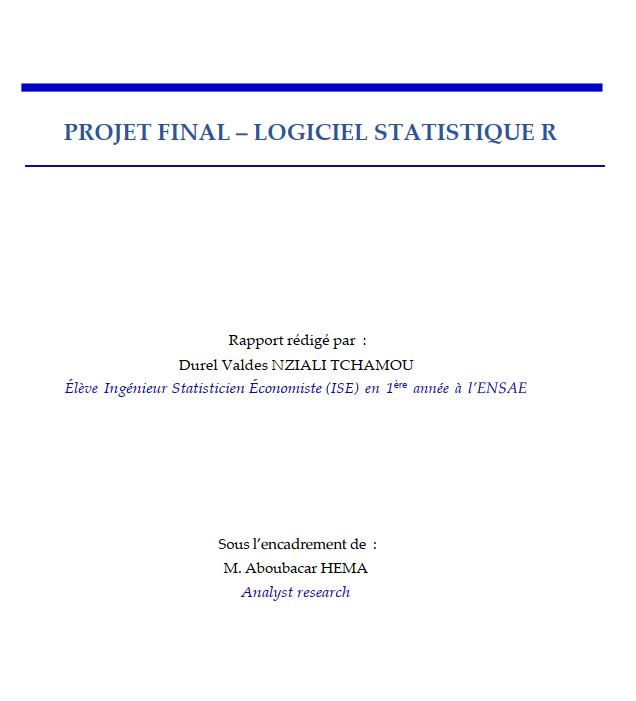
\includegraphics[width=7.61458in,height=\textheight]{assets/image3.png}

\hypertarget{importation-des-libraries-necessaires}{%
\paragraph{Importation des libraries
necessaires}\label{importation-des-libraries-necessaires}}

\begin{Shaded}
\begin{Highlighting}[]
\FunctionTok{library}\NormalTok{(readxl)}
\FunctionTok{library}\NormalTok{(dplyr)}
\FunctionTok{library}\NormalTok{(questionr)}
\FunctionTok{library}\NormalTok{(gtsummary)}
\FunctionTok{library}\NormalTok{(gt)}
\FunctionTok{library}\NormalTok{(webshot)}
\FunctionTok{library}\NormalTok{(ggplot2)}
\FunctionTok{library}\NormalTok{(sf)}
\FunctionTok{library}\NormalTok{(ggpubr)}
\FunctionTok{library}\NormalTok{(ggspatial)}
\FunctionTok{library}\NormalTok{(datawizard)}
\FunctionTok{library}\NormalTok{(kableExtra)}
\FunctionTok{library}\NormalTok{(janitor)}
\FunctionTok{library}\NormalTok{(flextable)}

\FunctionTok{library}\NormalTok{(htmlwidgets)}
\FunctionTok{library}\NormalTok{(webshot)}
\FunctionTok{library}\NormalTok{(knitr)}
\FunctionTok{library}\NormalTok{(lubridate)}
\FunctionTok{library}\NormalTok{(gridExtra)}
\FunctionTok{library}\NormalTok{(ggExtra)}
\end{Highlighting}
\end{Shaded}

\hypertarget{partie-1}{%
\section{Partie 1}\label{partie-1}}

\hypertarget{pruxe9paration-des-donnuxe9es}{%
\subsection{1. Préparation des
données}\label{pruxe9paration-des-donnuxe9es}}

\hypertarget{description}{%
\subsubsection{1.1. Description}\label{description}}

Une description exhaustive des variables a été faite dans le document
soumit à notre analyse.

\hypertarget{importation-et-mise-en-forme}{%
\subsubsection{1.2. Importation et mise en
forme}\label{importation-et-mise-en-forme}}

\begin{itemize}
\tightlist
\item
  Importer la base de données dans un objet de type
  \textbf{\emph{data.frame}} nommé \textbf{\emph{projet}}
\end{itemize}

\begin{Shaded}
\begin{Highlighting}[]
\NormalTok{projet }\OtherTok{\textless{}{-}} \FunctionTok{read\_excel}\NormalTok{(}\StringTok{"data/Base\_Partie 1.xlsx"}\NormalTok{)}
\end{Highlighting}
\end{Shaded}

\begin{itemize}
\tightlist
\item
  Observation préliminaire néccesaire qui porte sur l'analyse des
  doublons
\end{itemize}

\begin{Shaded}
\begin{Highlighting}[]
\DocumentationTok{\#\# vérifications des doublons}

\NormalTok{projet }\SpecialCharTok{\%\textgreater{}\%} 
  \FunctionTok{duplicated}\NormalTok{() }\SpecialCharTok{\%\textgreater{}\%} 
    \FunctionTok{table}\NormalTok{() }\SpecialCharTok{\%\textgreater{}\%}
       \FunctionTok{kbl}\NormalTok{()}
\end{Highlighting}
\end{Shaded}

\begin{tabular}[t]{l|r}
\hline
. & Freq\\
\hline
FALSE & 250\\
\hline
\end{tabular}

il n y a pas de doublons

\begin{itemize}
\tightlist
\item
  Selection des variables mentionnées dans la section description.
\end{itemize}

Il est important de noté que notre base ne contient que des variables
décrites dans la section de description.

\begin{itemize}
\tightlist
\item
  Visualisation graphique d'un résumé des valeurs manquantes par
  variable
\end{itemize}

\begin{Shaded}
\begin{Highlighting}[]
\CommentTok{\#graphique des valeurs manquantes}
\NormalTok{visdat}\SpecialCharTok{::}\FunctionTok{vis\_miss}\NormalTok{(projet)}
\end{Highlighting}
\end{Shaded}

\begin{figure}[H]

{\centering 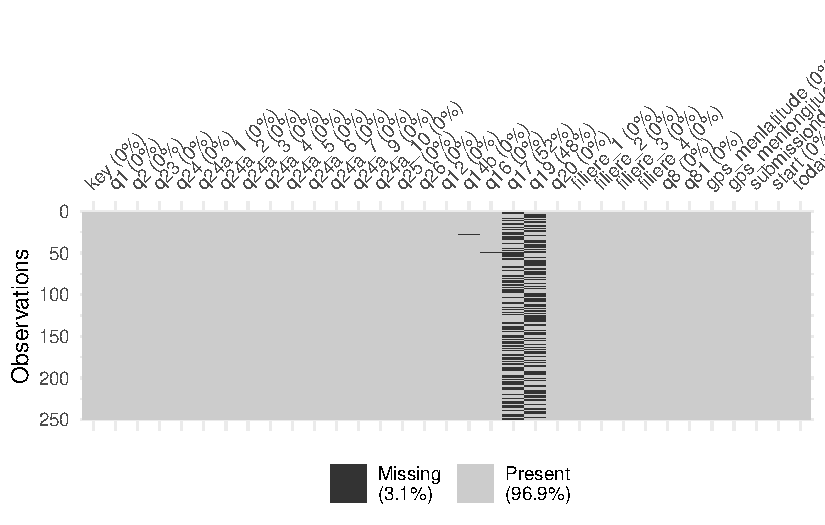
\includegraphics{projet_R_files/figure-pdf/unnamed-chunk-6-1.pdf}

}

\end{figure}

une premiere analyse serait de se dire que les Variables labelisés
\emph{\textbf{Autorisation de fabrication et de mise en vente} et}
\emph{\textbf{L'entreprise est-elle désservie par une route bitumée ?}
ont chacune 1 valeur manquante. et que} ~celles labelisés
\textbf{\emph{Etat de la route bitumée}} et \emph{\textbf{l'état de la
piste qui mène à l'entreprise} porte a elle deux près de 52\% et 48\%
des valeurs manquantes respectivement.\\
Cependant,} au regard de leur description de la base
(q17=\textbf{\emph{Etat de la route bitumée}} et
q19=\textbf{\emph{l'état de la piste qui mène à l'entreprise}})
présentent \textbf{\emph{des hors champs et non des valeurs
manquantes}}.

\begin{itemize}
\tightlist
\item
  Présentation sous forme de tableau un résumé des valeurs manquantes
  par variable
\end{itemize}

\begin{Shaded}
\begin{Highlighting}[]
\CommentTok{\# Calculer le nombre de valeurs manquantes par variable}

\NormalTok{projet }\SpecialCharTok{\%\textgreater{}\%}
    \FunctionTok{is.na}\NormalTok{() }\SpecialCharTok{\%\textgreater{}\%}                \CommentTok{\# Detection des valeurs manquantes}
      \FunctionTok{colSums}\NormalTok{() }\SpecialCharTok{\%\textgreater{}\%}            \CommentTok{\# sommes des vqleurs pqr colonne}
         \FunctionTok{sort}\NormalTok{(}\AttributeTok{decreasing =} \ConstantTok{TRUE}\NormalTok{) }\SpecialCharTok{\%\textgreater{}\%} \CommentTok{\# ranger par ordre décroissant}
            \FunctionTok{as.data.frame}\NormalTok{() }\SpecialCharTok{\%\textgreater{}\%}
              \FunctionTok{setNames}\NormalTok{(}\StringTok{"valeurs\_manquantes"}\NormalTok{) }\SpecialCharTok{\%\textgreater{}\%}  \CommentTok{\# donner un nom a la colonne du dataframe}
                \FunctionTok{mutate}\NormalTok{(}\AttributeTok{pourcentage =} \FunctionTok{round}\NormalTok{(valeurs\_manquantes }\SpecialCharTok{/} \FunctionTok{sum}\NormalTok{(valeurs\_manquantes, }\AttributeTok{na.rm =} \ConstantTok{TRUE}\NormalTok{) }\SpecialCharTok{*} \DecValTok{100}\NormalTok{, }\DecValTok{2}\NormalTok{)) }\SpecialCharTok{\%\textgreater{}\%}
                  \FunctionTok{kbl}\NormalTok{() }\SpecialCharTok{\%\textgreater{}\%} 
                    \FunctionTok{kable\_paper}\NormalTok{(}\AttributeTok{full\_width =} \ConstantTok{TRUE}\NormalTok{)}\SpecialCharTok{\%\textgreater{}\%}
                      \FunctionTok{row\_spec}\NormalTok{(}\DecValTok{1}\SpecialCharTok{:}\DecValTok{3}\NormalTok{, }\AttributeTok{background =} \StringTok{"red"}\NormalTok{) }\SpecialCharTok{\%\textgreater{}\%} 
                        \FunctionTok{row\_spec}\NormalTok{(}\DecValTok{3}\SpecialCharTok{:}\DecValTok{4}\NormalTok{, }\AttributeTok{background =} \StringTok{"lightblue"}\NormalTok{)}
\end{Highlighting}
\end{Shaded}

\begin{tabu} to \linewidth {>{\raggedright}X>{\raggedleft}X>{\raggedleft}X}
\hline
  & valeurs\_manquantes & pourcentage\\
\hline
\cellcolor{red}{q17} & \cellcolor{red}{131} & \cellcolor{red}{51.78}\\
\hline
\cellcolor{red}{q19} & \cellcolor{red}{120} & \cellcolor{red}{47.43}\\
\hline
\cellcolor{lightblue}{q14b} & \cellcolor{lightblue}{1} & \cellcolor{lightblue}{0.40}\\
\hline
\cellcolor{lightblue}{q16} & \cellcolor{lightblue}{1} & \cellcolor{lightblue}{0.40}\\
\hline
key & 0 & 0.00\\
\hline
q1 & 0 & 0.00\\
\hline
q2 & 0 & 0.00\\
\hline
q23 & 0 & 0.00\\
\hline
q24 & 0 & 0.00\\
\hline
q24a\_1 & 0 & 0.00\\
\hline
q24a\_2 & 0 & 0.00\\
\hline
q24a\_3 & 0 & 0.00\\
\hline
q24a\_4 & 0 & 0.00\\
\hline
q24a\_5 & 0 & 0.00\\
\hline
q24a\_6 & 0 & 0.00\\
\hline
q24a\_7 & 0 & 0.00\\
\hline
q24a\_9 & 0 & 0.00\\
\hline
q24a\_10 & 0 & 0.00\\
\hline
q25 & 0 & 0.00\\
\hline
q26 & 0 & 0.00\\
\hline
q12 & 0 & 0.00\\
\hline
q20 & 0 & 0.00\\
\hline
filiere\_1 & 0 & 0.00\\
\hline
filiere\_2 & 0 & 0.00\\
\hline
filiere\_3 & 0 & 0.00\\
\hline
filiere\_4 & 0 & 0.00\\
\hline
q8 & 0 & 0.00\\
\hline
q81 & 0 & 0.00\\
\hline
gps\_menlatitude & 0 & 0.00\\
\hline
gps\_menlongitude & 0 & 0.00\\
\hline
submissiondate & 0 & 0.00\\
\hline
start & 0 & 0.00\\
\hline
today & 0 & 0.00\\
\hline
\end{tabu}

Ce tableau vient confirmer les analyses faites plus hauts sur le concept
de valeur manquante et de hors champs.

\hfill\break
\textbf{\emph{Note :}} le faite de colorier les 4 premieres lignes est
la pour faciliter la présentation des données puisque avec l'observation
graphique précédente on avait déjà une vision exhaustive de ce qui etait
cherché

\begin{itemize}
\tightlist
\item
  Vérification s'il y a des valeurs manquantes pour la variable key dans
  la base projet. Si c'est effectivement le cas , l'on identifira la (ou
  les) PME concernée(s).
\end{itemize}

\begin{Shaded}
\begin{Highlighting}[]
\NormalTok{projet }\SpecialCharTok{\%\textgreater{}\%} 
  \FunctionTok{filter}\NormalTok{(}\FunctionTok{is.na}\NormalTok{(key)) }\SpecialCharTok{\%\textgreater{}\%} 
       \FunctionTok{kbl}\NormalTok{() }\SpecialCharTok{\%\textgreater{}\%} 
         \FunctionTok{kable\_paper}\NormalTok{(}\AttributeTok{full\_width =} \ConstantTok{TRUE}\NormalTok{)}
\end{Highlighting}
\end{Shaded}

\begin{tabu} to \linewidth {>{\raggedright}X>{\raggedright}X>{\raggedright}X>{\raggedright}X>{\raggedleft}X>{\raggedleft}X>{\raggedleft}X>{\raggedleft}X>{\raggedleft}X>{\raggedleft}X>{\raggedleft}X>{\raggedleft}X>{\raggedleft}X>{\raggedleft}X>{\raggedright}X>{\raggedleft}X>{\raggedright}X>{\raggedright}X>{\raggedright}X>{\raggedright}X>{\raggedright}X>{\raggedright}X>{\raggedleft}X>{\raggedleft}X>{\raggedleft}X>{\raggedleft}X>{\raggedright}X>{\raggedright}X>{\raggedleft}X>{\raggedleft}X>{\raggedright}X>{\raggedright}X>{\raggedright}X}
\hline
key & q1 & q2 & q23 & q24 & q24a\_1 & q24a\_2 & q24a\_3 & q24a\_4 & q24a\_5 & q24a\_6 & q24a\_7 & q24a\_9 & q24a\_10 & q25 & q26 & q12 & q14b & q16 & q17 & q19 & q20 & filiere\_1 & filiere\_2 & filiere\_3 & filiere\_4 & q8 & q81 & gps\_menlatitude & gps\_menlongitude & submissiondate & start & today\\


\hline
\end{tabu}

D'après le point précédent, la variable key n'a pas de valeurs
manquantes.

\hypertarget{cruxe9ation-de-variables}{%
\subsubsection{1.3. Création de
variables}\label{cruxe9ation-de-variables}}

\begin{itemize}
\tightlist
\item
  Rénommer les variables q1 en \emph{region} , q2 en \emph{departement}
  et q23 en \emph{sexe}.
\end{itemize}

\begin{Shaded}
\begin{Highlighting}[]
\CommentTok{\# Renommer les variables q1, q2 et q23}
\NormalTok{projet }\OtherTok{\textless{}{-}}\NormalTok{ projet }\SpecialCharTok{\%\textgreater{}\%}
              \FunctionTok{rename}\NormalTok{(}\AttributeTok{region =}\NormalTok{ q1, }\AttributeTok{departement =}\NormalTok{ q2, }\AttributeTok{sexe =}\NormalTok{ q23)}
\end{Highlighting}
\end{Shaded}

\begin{itemize}
\tightlist
\item
  Créer la variable sexe\_2 qui vaut 1 si sexe égale à Femme et 0 sinon.
\end{itemize}

\begin{Shaded}
\begin{Highlighting}[]
\CommentTok{\# Créer la variable sexe\_2}
\NormalTok{projet }\OtherTok{\textless{}{-}}\NormalTok{ projet }\SpecialCharTok{\%\textgreater{}\%} 
              \FunctionTok{mutate}\NormalTok{(}\AttributeTok{sexe\_2=}\FunctionTok{ifelse}\NormalTok{(projet}\SpecialCharTok{$}\NormalTok{sexe }\SpecialCharTok{==} \StringTok{"Femme"}\NormalTok{, }\DecValTok{1}\NormalTok{, }\DecValTok{0}\NormalTok{) )}
\end{Highlighting}
\end{Shaded}

\begin{itemize}
\tightlist
\item
  Créer un data.frame nommé langues qui prend les variables key et les
  variables correspondantes décrites plus haut. Indication: Vous
  remarquerez que ces variables commencent par q24a\_.
\end{itemize}

\begin{Shaded}
\begin{Highlighting}[]
\CommentTok{\#Créer le dataframe langues}
\NormalTok{langues}\OtherTok{\textless{}{-}}\NormalTok{projet }\SpecialCharTok{\%\textgreater{}\%} 
            \FunctionTok{select}\NormalTok{(key, }\FunctionTok{starts\_with}\NormalTok{(}\StringTok{"q24a\_"}\NormalTok{))}
\end{Highlighting}
\end{Shaded}

\begin{itemize}
\tightlist
\item
  Créer une variable parle qui est égale au nombre de langue parlée par
  le dirigeant de la PME.
\end{itemize}

\begin{Shaded}
\begin{Highlighting}[]
\CommentTok{\# Créer la variable "parle" en calculant la somme des réponses}
\NormalTok{langues }\OtherTok{\textless{}{-}}\NormalTok{ langues }\SpecialCharTok{\%\textgreater{}\%} 
                \FunctionTok{mutate}\NormalTok{(}\AttributeTok{parle =} \FunctionTok{rowSums}\NormalTok{(}\FunctionTok{select}\NormalTok{(., }\FunctionTok{starts\_with}\NormalTok{(}\StringTok{"q24a\_"}\NormalTok{))))}
\end{Highlighting}
\end{Shaded}

\begin{itemize}
\tightlist
\item
  Sélectionnez uniquement les variables key et parle, l'objet de retour
  sera langues.
\end{itemize}

\begin{Shaded}
\begin{Highlighting}[]
\NormalTok{langues }\OtherTok{\textless{}{-}}\NormalTok{ langues }\SpecialCharTok{\%\textgreater{}\%} 
                \FunctionTok{select}\NormalTok{(key, parle)}
\end{Highlighting}
\end{Shaded}

\begin{itemize}
\tightlist
\item
  Merger les data.frame projet et langues
\end{itemize}

\begin{Shaded}
\begin{Highlighting}[]
\NormalTok{projet}\OtherTok{\textless{}{-}}\FunctionTok{merge}\NormalTok{(projet, langues,}\AttributeTok{key\_vars=}\NormalTok{key)}
\end{Highlighting}
\end{Shaded}

\ul{\textbf{Note:}} Cette partie sur la langue il etait aussi possible
de le faire en \textbf{\emph{une seule ligne de code}}. le code reduit
est donc\\

\begin{Shaded}
\begin{Highlighting}[]
\NormalTok{projet}\OtherTok{\textless{}{-}}\NormalTok{projet }\SpecialCharTok{\%\textgreater{}\%} 
            \FunctionTok{mutate}\NormalTok{(}\AttributeTok{parle2 =} \FunctionTok{rowSums}\NormalTok{(}\FunctionTok{select}\NormalTok{(., }\FunctionTok{starts\_with}\NormalTok{(}\StringTok{"q24a\_"}\NormalTok{))))}
\end{Highlighting}
\end{Shaded}

\hypertarget{analyses-descriptives}{%
\subsection{2. Analyses descriptives}\label{analyses-descriptives}}

\hypertarget{statistiques-descriptives-univariuxe9es}{%
\subsubsection{2.1. Statistiques Descriptives
Univariées}\label{statistiques-descriptives-univariuxe9es}}

\hypertarget{tableaux-statistiques}{%
\paragraph{2.1.1. Tableaux statistiques}\label{tableaux-statistiques}}

Quelle est la répartion des PME suivant:

\begin{itemize}
\item
  le sexe?
\item
  le niveau d'instruction?
\item
  le statut juridique?
\item
  le propriétaire/locataire?
\end{itemize}

\begin{Shaded}
\begin{Highlighting}[]
\CommentTok{\# Répartition des PME suivant ces variables}
\NormalTok{tab2 }\OtherTok{=}\NormalTok{  projet }\SpecialCharTok{\%\textgreater{}\%}
                  \FunctionTok{select}\NormalTok{(sexe, q25,q12,q81) }\SpecialCharTok{\%\textgreater{}\%}
                      \FunctionTok{rename}\NormalTok{(}\StringTok{"Niveau d’instruction du dirigeant/responsable de la PME"} \OtherTok{=}\NormalTok{ q25, }\StringTok{"Statut juridique*"}\OtherTok{=}\NormalTok{q12, }\StringTok{"*propriétaire ou locataire"}\OtherTok{=}\NormalTok{q81) }\SpecialCharTok{\%\textgreater{}\%} 
                         \FunctionTok{tbl\_summary}\NormalTok{()}\SpecialCharTok{\%\textgreater{}\%}
                                \FunctionTok{modify\_spanning\_header}\NormalTok{(}\FunctionTok{everything}\NormalTok{() }\SpecialCharTok{\textasciitilde{}} \StringTok{"**Répartition des PME selon les variables**"}\NormalTok{) }\SpecialCharTok{\%\textgreater{}\%} 
                                        \FunctionTok{bold\_labels}\NormalTok{()}

\NormalTok{tab2}\SpecialCharTok{\%\textgreater{}\%} \FunctionTok{bold\_labels}\NormalTok{() }\SpecialCharTok{\%\textgreater{}\%} 
  \FunctionTok{italicize\_levels}\NormalTok{()  }\SpecialCharTok{\%\textgreater{}\%} 
  \FunctionTok{modify\_header}\NormalTok{(}\AttributeTok{update =} \FunctionTok{list}\NormalTok{( label }\SpecialCharTok{\textasciitilde{}} \StringTok{"**VARIABLE**"}\NormalTok{, }\FunctionTok{all\_stat\_cols}\NormalTok{(}\AttributeTok{stat\_0 =} \ConstantTok{FALSE}\NormalTok{) }\SpecialCharTok{\textasciitilde{}} \StringTok{"**\{level\}** (n=\{n\}, \{style\_percent(p)\}\%)"}
\NormalTok{  )) }\SpecialCharTok{\%\textgreater{}\%}  \FunctionTok{as\_flex\_table}\NormalTok{() }\SpecialCharTok{\%\textgreater{}\%}
             \FunctionTok{fontsize}\NormalTok{(}\AttributeTok{size =} \DecValTok{8}\NormalTok{)}\SpecialCharTok{\%\textgreater{}\%}
                   \FunctionTok{width}\NormalTok{(}\AttributeTok{width =} \FloatTok{1.65}\NormalTok{) }
\end{Highlighting}
\end{Shaded}

\ul{\textbf{\emph{Commentaire :}}} La plupart des PME sont dans des GIE
ou exercent dans le secteur informel. Les dirigeants des PME sont en
majorité des propriétaires, environ 90\%. On constate aussi que tres peu
d'entre eux ont un niveau supérieur .une analyse par la filière nous
donnera certainement plus de précision.\\
\strut \\
Avant d'aller plus loin il est important de faire d'observer la
repartition des PME par filière :

\begin{Shaded}
\begin{Highlighting}[]
\CommentTok{\# répartition des PME par filière}
\NormalTok{tab3}\OtherTok{=}\NormalTok{ projet }\SpecialCharTok{\%\textgreater{}\%}
          \FunctionTok{select}\NormalTok{(}\FunctionTok{starts\_with}\NormalTok{(}\StringTok{"filiere\_"}\NormalTok{)) }\SpecialCharTok{\%\textgreater{}\%}
               \FunctionTok{tbl\_summary}\NormalTok{( }\AttributeTok{missing =} \StringTok{"no"}\NormalTok{)}\SpecialCharTok{\%\textgreater{}\%} 
                    \FunctionTok{bold\_labels}\NormalTok{()}

\NormalTok{tab3}\SpecialCharTok{\%\textgreater{}\%} \FunctionTok{bold\_labels}\NormalTok{() }\SpecialCharTok{\%\textgreater{}\%} 
  \FunctionTok{italicize\_levels}\NormalTok{()  }\SpecialCharTok{\%\textgreater{}\%} 
  \FunctionTok{modify\_header}\NormalTok{(}\AttributeTok{update =} \FunctionTok{list}\NormalTok{( label }\SpecialCharTok{\textasciitilde{}} \StringTok{"**VARIABLE**"}\NormalTok{, }\FunctionTok{all\_stat\_cols}\NormalTok{(}\AttributeTok{stat\_0 =} \ConstantTok{FALSE}\NormalTok{) }\SpecialCharTok{\textasciitilde{}} \StringTok{"**\{level\}** (n=\{n\}, \{style\_percent(p)\}\%)"}
\NormalTok{  )) }\SpecialCharTok{\%\textgreater{}\%}  \FunctionTok{as\_flex\_table}\NormalTok{() }\SpecialCharTok{\%\textgreater{}\%}
  \FunctionTok{fontsize}\NormalTok{(}\AttributeTok{size =} \DecValTok{8}\NormalTok{) }\SpecialCharTok{\%\textgreater{}\%}
  \FunctionTok{width}\NormalTok{(}\AttributeTok{width =} \FloatTok{1.65}\NormalTok{)}
\end{Highlighting}
\end{Shaded}

\global\setlength{\Oldarrayrulewidth}{\arrayrulewidth}

\global\setlength{\Oldtabcolsep}{\tabcolsep}

\setlength{\tabcolsep}{0pt}

\renewcommand*{\arraystretch}{1.5}



\providecommand{\ascline}[3]{\noalign{\global\arrayrulewidth #1}\arrayrulecolor[HTML]{#2}\cline{#3}}

\begin{longtable*}[c]{|p{1.65in}|p{1.65in}}



\ascline{1pt}{000000}{1-2}

\multicolumn{1}{>{\raggedright}m{\dimexpr 1.65in+0\tabcolsep}}{\textcolor[HTML]{000000}{\fontsize{11}{11}\selectfont{\textbf{VARIABLE}}}} & \multicolumn{1}{>{\centering}m{\dimexpr 1.65in+0\tabcolsep}}{\textcolor[HTML]{000000}{\fontsize{11}{11}\selectfont{\textbf{N\ =\ 250}}}\textcolor[HTML]{000000}{\textsuperscript{\fontsize{11}{11}\selectfont{1}}}} \\

\ascline{1pt}{000000}{1-2}\endfirsthead 

\ascline{1pt}{000000}{1-2}

\multicolumn{1}{>{\raggedright}m{\dimexpr 1.65in+0\tabcolsep}}{\textcolor[HTML]{000000}{\fontsize{11}{11}\selectfont{\textbf{VARIABLE}}}} & \multicolumn{1}{>{\centering}m{\dimexpr 1.65in+0\tabcolsep}}{\textcolor[HTML]{000000}{\fontsize{11}{11}\selectfont{\textbf{N\ =\ 250}}}\textcolor[HTML]{000000}{\textsuperscript{\fontsize{11}{11}\selectfont{1}}}} \\

\ascline{1pt}{000000}{1-2}\endhead



\multicolumn{1}{>{\raggedright}p{\dimexpr 1.65in+0\tabcolsep}}{\textcolor[HTML]{000000}{\fontsize{8}{8}\selectfont{\textbf{filiere\_1}}}} & \multicolumn{1}{>{\centering}p{\dimexpr 1.65in+0\tabcolsep}}{\textcolor[HTML]{000000}{\fontsize{8}{8}\selectfont{108\ (43\%)}}} \\





\multicolumn{1}{>{\raggedright}p{\dimexpr 1.65in+0\tabcolsep}}{\textcolor[HTML]{000000}{\fontsize{8}{8}\selectfont{\textbf{filiere\_2}}}} & \multicolumn{1}{>{\centering}p{\dimexpr 1.65in+0\tabcolsep}}{\textcolor[HTML]{000000}{\fontsize{8}{8}\selectfont{61\ (24\%)}}} \\





\multicolumn{1}{>{\raggedright}p{\dimexpr 1.65in+0\tabcolsep}}{\textcolor[HTML]{000000}{\fontsize{8}{8}\selectfont{\textbf{filiere\_3}}}} & \multicolumn{1}{>{\centering}p{\dimexpr 1.65in+0\tabcolsep}}{\textcolor[HTML]{000000}{\fontsize{8}{8}\selectfont{89\ (36\%)}}} \\





\multicolumn{1}{>{\raggedright}p{\dimexpr 1.65in+0\tabcolsep}}{\textcolor[HTML]{000000}{\fontsize{8}{8}\selectfont{\textbf{filiere\_4}}}} & \multicolumn{1}{>{\centering}p{\dimexpr 1.65in+0\tabcolsep}}{\textcolor[HTML]{000000}{\fontsize{8}{8}\selectfont{92\ (37\%)}}} \\

\ascline{1pt}{000000}{1-2}



\multicolumn{2}{>{\raggedright}m{\dimexpr 3.3in+2\tabcolsep}}{\textcolor[HTML]{000000}{\textsuperscript{\fontsize{11}{11}\selectfont{1}}}\textcolor[HTML]{000000}{\fontsize{11}{11}\selectfont{n\ (\%)}}} \\





\end{longtable*}



\arrayrulecolor[HTML]{000000}

\global\setlength{\arrayrulewidth}{\Oldarrayrulewidth}

\global\setlength{\tabcolsep}{\Oldtabcolsep}

\renewcommand*{\arraystretch}{1}

\hfill\break
Maintenant que nous savons la repartition des PME par filière, on se
demande ce qu'il en est de la répartition des PME par nombre de filière
dans laquelle agit les PME.

\begin{Shaded}
\begin{Highlighting}[]
\CommentTok{\# répartition des PME par nombre de filière dans laquelle agit les PME}

\NormalTok{tab4 }\OtherTok{=}\NormalTok{ projet }\SpecialCharTok{\%\textgreater{}\%} 
             \FunctionTok{mutate}\NormalTok{(}\AttributeTok{filiere =} \FunctionTok{as.factor}\NormalTok{(}\FunctionTok{rowSums}\NormalTok{(}\FunctionTok{select}\NormalTok{(., }\FunctionTok{starts\_with}\NormalTok{(}\StringTok{"filiere\_"}\NormalTok{))))) }\SpecialCharTok{\%\textgreater{}\%}           \FunctionTok{select}\NormalTok{(filiere) }\SpecialCharTok{\%\textgreater{}\%} 
                       \FunctionTok{tbl\_summary}\NormalTok{( }\AttributeTok{missing =} \StringTok{"no"}\NormalTok{)}\SpecialCharTok{\%\textgreater{}\%} 
                          \FunctionTok{bold\_labels}\NormalTok{()}

\NormalTok{tab4}\SpecialCharTok{\%\textgreater{}\%} \FunctionTok{bold\_labels}\NormalTok{() }\SpecialCharTok{\%\textgreater{}\%} 
  \FunctionTok{italicize\_levels}\NormalTok{()  }\SpecialCharTok{\%\textgreater{}\%} 
  \FunctionTok{modify\_header}\NormalTok{(}\AttributeTok{update =} \FunctionTok{list}\NormalTok{( label }\SpecialCharTok{\textasciitilde{}} \StringTok{"**VARIABLE**"}\NormalTok{, }\FunctionTok{all\_stat\_cols}\NormalTok{(}\AttributeTok{stat\_0 =} \ConstantTok{FALSE}\NormalTok{) }\SpecialCharTok{\textasciitilde{}} \StringTok{"**\{level\}** (n=\{n\}, \{style\_percent(p)\}\%)"}
\NormalTok{  )) }\SpecialCharTok{\%\textgreater{}\%}  \FunctionTok{as\_flex\_table}\NormalTok{() }\SpecialCharTok{\%\textgreater{}\%}
  \FunctionTok{fontsize}\NormalTok{(}\AttributeTok{size =} \DecValTok{8}\NormalTok{) }\SpecialCharTok{\%\textgreater{}\%}
  \FunctionTok{width}\NormalTok{(}\AttributeTok{width =} \FloatTok{1.65}\NormalTok{)}
\end{Highlighting}
\end{Shaded}

\global\setlength{\Oldarrayrulewidth}{\arrayrulewidth}

\global\setlength{\Oldtabcolsep}{\tabcolsep}

\setlength{\tabcolsep}{0pt}

\renewcommand*{\arraystretch}{1.5}



\providecommand{\ascline}[3]{\noalign{\global\arrayrulewidth #1}\arrayrulecolor[HTML]{#2}\cline{#3}}

\begin{longtable*}[c]{|p{1.65in}|p{1.65in}}



\ascline{1pt}{000000}{1-2}

\multicolumn{1}{>{\raggedright}m{\dimexpr 1.65in+0\tabcolsep}}{\textcolor[HTML]{000000}{\fontsize{11}{11}\selectfont{\textbf{VARIABLE}}}} & \multicolumn{1}{>{\centering}m{\dimexpr 1.65in+0\tabcolsep}}{\textcolor[HTML]{000000}{\fontsize{11}{11}\selectfont{\textbf{N\ =\ 250}}}\textcolor[HTML]{000000}{\textsuperscript{\fontsize{11}{11}\selectfont{1}}}} \\

\ascline{1pt}{000000}{1-2}\endfirsthead 

\ascline{1pt}{000000}{1-2}

\multicolumn{1}{>{\raggedright}m{\dimexpr 1.65in+0\tabcolsep}}{\textcolor[HTML]{000000}{\fontsize{11}{11}\selectfont{\textbf{VARIABLE}}}} & \multicolumn{1}{>{\centering}m{\dimexpr 1.65in+0\tabcolsep}}{\textcolor[HTML]{000000}{\fontsize{11}{11}\selectfont{\textbf{N\ =\ 250}}}\textcolor[HTML]{000000}{\textsuperscript{\fontsize{11}{11}\selectfont{1}}}} \\

\ascline{1pt}{000000}{1-2}\endhead



\multicolumn{1}{>{\raggedright}p{\dimexpr 1.65in+0\tabcolsep}}{\textcolor[HTML]{000000}{\fontsize{8}{8}\selectfont{\textbf{filiere}}}} & \multicolumn{1}{>{\centering}p{\dimexpr 1.65in+0\tabcolsep}}{\textcolor[HTML]{000000}{\fontsize{8}{8}\selectfont{}}} \\





\multicolumn{1}{>{\raggedright}p{\dimexpr 1.65in+0\tabcolsep}}{\textcolor[HTML]{000000}{\fontsize{8}{8}\selectfont{\textit{1}}}} & \multicolumn{1}{>{\centering}p{\dimexpr 1.65in+0\tabcolsep}}{\textcolor[HTML]{000000}{\fontsize{8}{8}\selectfont{171\ (68\%)}}} \\





\multicolumn{1}{>{\raggedright}p{\dimexpr 1.65in+0\tabcolsep}}{\textcolor[HTML]{000000}{\fontsize{8}{8}\selectfont{\textit{2}}}} & \multicolumn{1}{>{\centering}p{\dimexpr 1.65in+0\tabcolsep}}{\textcolor[HTML]{000000}{\fontsize{8}{8}\selectfont{59\ (24\%)}}} \\





\multicolumn{1}{>{\raggedright}p{\dimexpr 1.65in+0\tabcolsep}}{\textcolor[HTML]{000000}{\fontsize{8}{8}\selectfont{\textit{3}}}} & \multicolumn{1}{>{\centering}p{\dimexpr 1.65in+0\tabcolsep}}{\textcolor[HTML]{000000}{\fontsize{8}{8}\selectfont{19\ (7.6\%)}}} \\





\multicolumn{1}{>{\raggedright}p{\dimexpr 1.65in+0\tabcolsep}}{\textcolor[HTML]{000000}{\fontsize{8}{8}\selectfont{\textit{4}}}} & \multicolumn{1}{>{\centering}p{\dimexpr 1.65in+0\tabcolsep}}{\textcolor[HTML]{000000}{\fontsize{8}{8}\selectfont{1\ (0.4\%)}}} \\

\ascline{1pt}{000000}{1-2}



\multicolumn{2}{>{\raggedright}m{\dimexpr 3.3in+2\tabcolsep}}{\textcolor[HTML]{000000}{\textsuperscript{\fontsize{11}{11}\selectfont{1}}}\textcolor[HTML]{000000}{\fontsize{11}{11}\selectfont{n\ (\%)}}} \\





\end{longtable*}



\arrayrulecolor[HTML]{000000}

\global\setlength{\arrayrulewidth}{\Oldarrayrulewidth}

\global\setlength{\tabcolsep}{\Oldtabcolsep}

\renewcommand*{\arraystretch}{1}

il ressort d'une analyse rapide que certains entreprises sont dans
plusieurs filière à la fois. En effet \textbf{79} sont celles qui sont
dans au moins une filière. L'analyse approfondie nous révèle que
\textbf{59} d'entre elles sont dans deux ilières et une seule est dans
quatre filières.\\

\hypertarget{cruxe9ation-dune-variable-avec-le-nom-des-filiuxe8res}{%
\paragraph{2.1.2. Création d'une variable avec le nom des
filières}\label{cruxe9ation-dune-variable-avec-le-nom-des-filiuxe8res}}

\begin{Shaded}
\begin{Highlighting}[]
\CommentTok{\# creation d\textquotesingle{}une variable avec le nom des filière}
\NormalTok{projet}\OtherTok{\textless{}{-}}\NormalTok{ projet }\SpecialCharTok{\%\textgreater{}\%} 
            \FunctionTok{mutate}\NormalTok{(}\AttributeTok{filiere =} \FunctionTok{as.factor}\NormalTok{(}\FunctionTok{rowSums}\NormalTok{(}\FunctionTok{select}\NormalTok{(., }\FunctionTok{starts\_with}\NormalTok{(}\StringTok{"filiere\_"}\NormalTok{)))),}
                    \AttributeTok{nom\_filiere =} \FunctionTok{case\_when}\NormalTok{(}
\NormalTok{                                      filiere }\SpecialCharTok{==} \DecValTok{1} \SpecialCharTok{\&}\NormalTok{ filiere\_1}\SpecialCharTok{==}\DecValTok{1}\SpecialCharTok{\textasciitilde{}} \StringTok{"arachide"}\NormalTok{,}
\NormalTok{                                      filiere }\SpecialCharTok{==} \DecValTok{1} \SpecialCharTok{\&}\NormalTok{ filiere\_2}\SpecialCharTok{==}\DecValTok{1}\SpecialCharTok{\textasciitilde{}} \StringTok{"anacarde"}\NormalTok{,}
\NormalTok{                                      filiere }\SpecialCharTok{==} \DecValTok{1} \SpecialCharTok{\&}\NormalTok{ filiere\_3}\SpecialCharTok{==}\DecValTok{1}\SpecialCharTok{\textasciitilde{}} \StringTok{"mangue"}\NormalTok{,}
\NormalTok{                                      filiere }\SpecialCharTok{==} \DecValTok{1} \SpecialCharTok{\&}\NormalTok{ filiere\_4}\SpecialCharTok{==}\DecValTok{1}\SpecialCharTok{\textasciitilde{}} \StringTok{"riz"}\NormalTok{,}
\NormalTok{                                      filiere }\SpecialCharTok{==} \DecValTok{2} \SpecialCharTok{\&}\NormalTok{ (filiere\_1}\SpecialCharTok{==}\DecValTok{1} \SpecialCharTok{\&}\NormalTok{ filiere\_2}\SpecialCharTok{==}\DecValTok{1}\NormalTok{) }\SpecialCharTok{\textasciitilde{}} \StringTok{"arachide \& anacarde"}\NormalTok{,}
\NormalTok{                                      filiere }\SpecialCharTok{==} \DecValTok{2} \SpecialCharTok{\&}\NormalTok{ (filiere\_1}\SpecialCharTok{==}\DecValTok{1} \SpecialCharTok{\&}\NormalTok{ filiere\_3}\SpecialCharTok{==}\DecValTok{1}\NormalTok{) }\SpecialCharTok{\textasciitilde{}} \StringTok{"arachide \& mangue"}\NormalTok{,}
\NormalTok{                                      filiere }\SpecialCharTok{==} \DecValTok{2} \SpecialCharTok{\&}\NormalTok{ (filiere\_1}\SpecialCharTok{==}\DecValTok{1} \SpecialCharTok{\&}\NormalTok{ filiere\_4}\SpecialCharTok{==}\DecValTok{1}\NormalTok{) }\SpecialCharTok{\textasciitilde{}} \StringTok{"arachide \& riz"}\NormalTok{,}
\NormalTok{                                      filiere }\SpecialCharTok{==} \DecValTok{2} \SpecialCharTok{\&}\NormalTok{ (filiere\_2}\SpecialCharTok{==}\DecValTok{1} \SpecialCharTok{\&}\NormalTok{ filiere\_3}\SpecialCharTok{==}\DecValTok{1}\NormalTok{) }\SpecialCharTok{\textasciitilde{}} \StringTok{"mangue \& anacarde"}\NormalTok{,}
\NormalTok{                                      filiere }\SpecialCharTok{==} \DecValTok{2} \SpecialCharTok{\&}\NormalTok{ (filiere\_2}\SpecialCharTok{==}\DecValTok{1} \SpecialCharTok{\&}\NormalTok{ filiere\_4}\SpecialCharTok{==}\DecValTok{1}\NormalTok{) }\SpecialCharTok{\textasciitilde{}} \StringTok{"riz \& anacarde"}\NormalTok{,}
\NormalTok{                                      filiere }\SpecialCharTok{==} \DecValTok{2} \SpecialCharTok{\&}\NormalTok{ (filiere\_3}\SpecialCharTok{==}\DecValTok{1} \SpecialCharTok{\&}\NormalTok{ filiere\_4}\SpecialCharTok{==}\DecValTok{1}\NormalTok{) }\SpecialCharTok{\textasciitilde{}} \StringTok{"riz \& mangue"}\NormalTok{,}
\NormalTok{                                      filiere }\SpecialCharTok{==} \DecValTok{3} \SpecialCharTok{\&}\NormalTok{ (filiere\_1}\SpecialCharTok{==}\DecValTok{1} \SpecialCharTok{\&}\NormalTok{ filiere\_2}\SpecialCharTok{==}\DecValTok{1} \SpecialCharTok{\&}\NormalTok{ filiere\_3}\SpecialCharTok{==}\DecValTok{1}\NormalTok{)}\SpecialCharTok{\textasciitilde{}} \StringTok{"arachide \& anacarde \& mangue"}\NormalTok{,}
\NormalTok{                                      filiere }\SpecialCharTok{==} \DecValTok{3} \SpecialCharTok{\&}\NormalTok{ (filiere\_1}\SpecialCharTok{==}\DecValTok{1} \SpecialCharTok{\&}\NormalTok{ filiere\_2}\SpecialCharTok{==}\DecValTok{1} \SpecialCharTok{\&}\NormalTok{ filiere\_4}\SpecialCharTok{==}\DecValTok{1}\NormalTok{)}\SpecialCharTok{\textasciitilde{}} \StringTok{"arachide \& anacarde \& riz"}\NormalTok{,}
\NormalTok{                                      filiere }\SpecialCharTok{==} \DecValTok{3} \SpecialCharTok{\&}\NormalTok{ (filiere\_1}\SpecialCharTok{==}\DecValTok{1} \SpecialCharTok{\&}\NormalTok{ filiere\_4}\SpecialCharTok{==}\DecValTok{1} \SpecialCharTok{\&}\NormalTok{ filiere\_3}\SpecialCharTok{==}\DecValTok{1}\NormalTok{)}\SpecialCharTok{\textasciitilde{}} \StringTok{"arachide \& riz \& mangue"}\NormalTok{,}
\NormalTok{                                      filiere }\SpecialCharTok{==} \DecValTok{3} \SpecialCharTok{\&}\NormalTok{ (filiere\_4}\SpecialCharTok{==}\DecValTok{1} \SpecialCharTok{\&}\NormalTok{ filiere\_2}\SpecialCharTok{==}\DecValTok{1} \SpecialCharTok{\&}\NormalTok{ filiere\_3}\SpecialCharTok{==}\DecValTok{1}\NormalTok{)}\SpecialCharTok{\textasciitilde{}} \StringTok{"riz \& anacarde \& mangue"}\NormalTok{,}
\NormalTok{                                      filiere }\SpecialCharTok{==} \DecValTok{4} \SpecialCharTok{\&}\NormalTok{ (filiere\_1}\SpecialCharTok{==}\DecValTok{1} \SpecialCharTok{\&}\NormalTok{filiere\_4}\SpecialCharTok{==}\DecValTok{1} \SpecialCharTok{\&}\NormalTok{ filiere\_2}\SpecialCharTok{==}\DecValTok{1} \SpecialCharTok{\&}\NormalTok{ filiere\_3}\SpecialCharTok{==}\DecValTok{1}\NormalTok{)}\SpecialCharTok{\textasciitilde{}} \StringTok{"arachide \& anacarde \& mangue\& riz"}\NormalTok{,}
                                      \ConstantTok{TRUE} \SpecialCharTok{\textasciitilde{}} \StringTok{"Autre"}
\NormalTok{                                    ))}
\end{Highlighting}
\end{Shaded}

\hypertarget{ruxe9pruxe9sentation-graphique}{%
\paragraph{2.1.3. Réprésentation
graphique}\label{ruxe9pruxe9sentation-graphique}}

\begin{itemize}
\tightlist
\item
  Répartition des PME selon le sexe
\end{itemize}

\begin{Shaded}
\begin{Highlighting}[]
\CommentTok{\#sexe}

\CommentTok{\# Répartition des PME selon le sexe}
\NormalTok{pme\_repartition }\OtherTok{\textless{}{-}}\NormalTok{ projet }\SpecialCharTok{\%\textgreater{}\%}
  \FunctionTok{select}\NormalTok{(sexe) }\SpecialCharTok{\%\textgreater{}\%}
  \FunctionTok{count}\NormalTok{(sexe) }\SpecialCharTok{\%\textgreater{}\%}
  \FunctionTok{mutate}\NormalTok{(}\AttributeTok{percentage =}\NormalTok{ n }\SpecialCharTok{/} \FunctionTok{sum}\NormalTok{(n) }\SpecialCharTok{*} \DecValTok{100}\NormalTok{)  }\CommentTok{\# Calcul du pourcentage}

\CommentTok{\# Création du graphique en secteurs plein (pie chart) avec les pourcentages}
\FunctionTok{ggplot}\NormalTok{(pme\_repartition, }\FunctionTok{aes}\NormalTok{(}\AttributeTok{x =} \StringTok{""}\NormalTok{, }\AttributeTok{y =}\NormalTok{ n, }\AttributeTok{fill =}\NormalTok{ sexe)) }\SpecialCharTok{+}
  \FunctionTok{geom\_bar}\NormalTok{(}\AttributeTok{stat =} \StringTok{"identity"}\NormalTok{, }\AttributeTok{position =} \StringTok{"fill"}\NormalTok{) }\SpecialCharTok{+}
  \FunctionTok{coord\_polar}\NormalTok{(}\StringTok{"y"}\NormalTok{) }\SpecialCharTok{+}
  \FunctionTok{scale\_fill\_manual}\NormalTok{(}\AttributeTok{values =} \FunctionTok{c}\NormalTok{(}\StringTok{"\#E45756"}\NormalTok{, }\StringTok{"\#4C78A8"}\NormalTok{)) }\SpecialCharTok{+}  \CommentTok{\# Couleurs des secteurs (à personnaliser)}
  \FunctionTok{labs}\NormalTok{(}\AttributeTok{x =} \ConstantTok{NULL}\NormalTok{, }\AttributeTok{y =} \ConstantTok{NULL}\NormalTok{, }\AttributeTok{fill =} \StringTok{"Sexe"}\NormalTok{) }\SpecialCharTok{+}
  \FunctionTok{geom\_text}\NormalTok{(}\FunctionTok{aes}\NormalTok{(}\AttributeTok{label =} \FunctionTok{paste0}\NormalTok{(}\FunctionTok{round}\NormalTok{(percentage, }\DecValTok{1}\NormalTok{), }\StringTok{"\%"}\NormalTok{)), }\AttributeTok{position =} \FunctionTok{position\_fill}\NormalTok{(}\AttributeTok{vjust =} \FloatTok{0.5}\NormalTok{), }\AttributeTok{color =} \StringTok{"white"}\NormalTok{) }\SpecialCharTok{+}
  \FunctionTok{theme\_void}\NormalTok{()}\SpecialCharTok{+}
  \FunctionTok{labs}\NormalTok{(}\AttributeTok{title =} \StringTok{"Répartition des PME selon le sexe du dirigeant"}\NormalTok{)}
\end{Highlighting}
\end{Shaded}

\begin{figure}[H]

{\centering 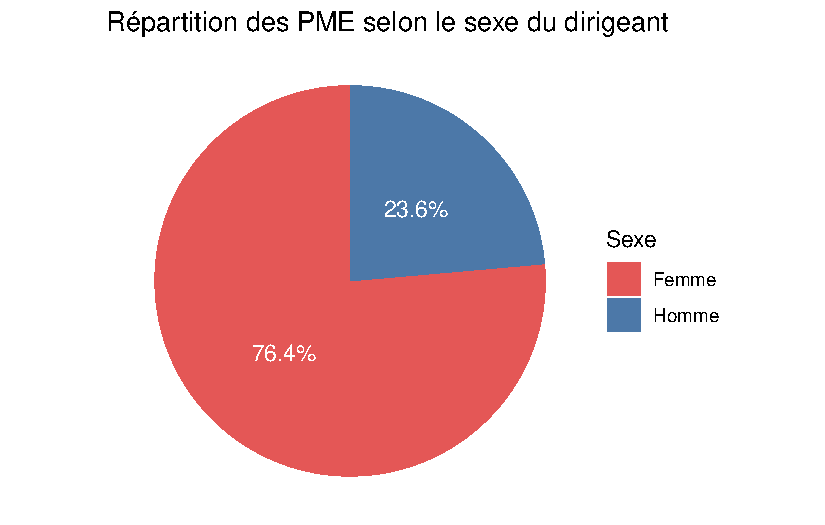
\includegraphics{projet_R_files/figure-pdf/unnamed-chunk-20-1.pdf}

}

\end{figure}

\begin{itemize}
\tightlist
\item
  Répartition des PME selon le niveau scolaire
\end{itemize}

\begin{Shaded}
\begin{Highlighting}[]
\CommentTok{\#q25}


\CommentTok{\# Répartition des PME selon le niveau scolaire}
\NormalTok{pme\_repartition }\OtherTok{\textless{}{-}}\NormalTok{ projet }\SpecialCharTok{\%\textgreater{}\%}
  \FunctionTok{select}\NormalTok{(q25) }\SpecialCharTok{\%\textgreater{}\%}
  \FunctionTok{count}\NormalTok{(q25) }\SpecialCharTok{\%\textgreater{}\%}
  \FunctionTok{mutate}\NormalTok{(}\AttributeTok{percentage =}\NormalTok{ n }\SpecialCharTok{/} \FunctionTok{sum}\NormalTok{(n) }\SpecialCharTok{*} \DecValTok{100}\NormalTok{)  }\CommentTok{\# Calcul du pourcentage}

\CommentTok{\# Création du graphique en secteurs plein avec les pourcentages}

\FunctionTok{ggplot}\NormalTok{(pme\_repartition, }\FunctionTok{aes}\NormalTok{(}\AttributeTok{x =} \StringTok{""}\NormalTok{, }\AttributeTok{y =}\NormalTok{ n, }\AttributeTok{fill =}\NormalTok{ q25)) }\SpecialCharTok{+}
  \FunctionTok{geom\_bar}\NormalTok{(}\AttributeTok{stat =} \StringTok{"identity"}\NormalTok{, }\AttributeTok{position =} \StringTok{"fill"}\NormalTok{) }\SpecialCharTok{+}
  \FunctionTok{coord\_polar}\NormalTok{(}\StringTok{"y"}\NormalTok{) }\SpecialCharTok{+}
  \FunctionTok{scale\_fill\_manual}\NormalTok{(}\AttributeTok{values =} \FunctionTok{c}\NormalTok{(}\StringTok{"\#E45756"}\NormalTok{, }\StringTok{"\#4C78A8"}\NormalTok{,}\StringTok{"darkgreen"}\NormalTok{,}\StringTok{"blue"}\NormalTok{)) }\SpecialCharTok{+}  \CommentTok{\# Couleurs des secteurs (à personnaliser)}
  \FunctionTok{labs}\NormalTok{(}\AttributeTok{x =} \ConstantTok{NULL}\NormalTok{, }\AttributeTok{y =} \ConstantTok{NULL}\NormalTok{, }\AttributeTok{fill =} \StringTok{"niveau d\textquotesingle{}instruction"}\NormalTok{) }\SpecialCharTok{+}
  \FunctionTok{geom\_text}\NormalTok{(}\FunctionTok{aes}\NormalTok{(}\AttributeTok{label =} \FunctionTok{paste0}\NormalTok{(}\FunctionTok{round}\NormalTok{(percentage, }\DecValTok{1}\NormalTok{), }\StringTok{"\%"}\NormalTok{)), }\AttributeTok{position =} \FunctionTok{position\_fill}\NormalTok{(}\AttributeTok{vjust =} \FloatTok{0.5}\NormalTok{), }\AttributeTok{color =} \StringTok{"white"}\NormalTok{) }\SpecialCharTok{+}
  \FunctionTok{theme\_void}\NormalTok{()}\SpecialCharTok{+}
  \FunctionTok{labs}\NormalTok{(}\AttributeTok{title =} \StringTok{"Répartition des PME selon le niveau d\textquotesingle{}instruction du dirigeant"}\NormalTok{)}
\end{Highlighting}
\end{Shaded}

\begin{figure}[H]

{\centering 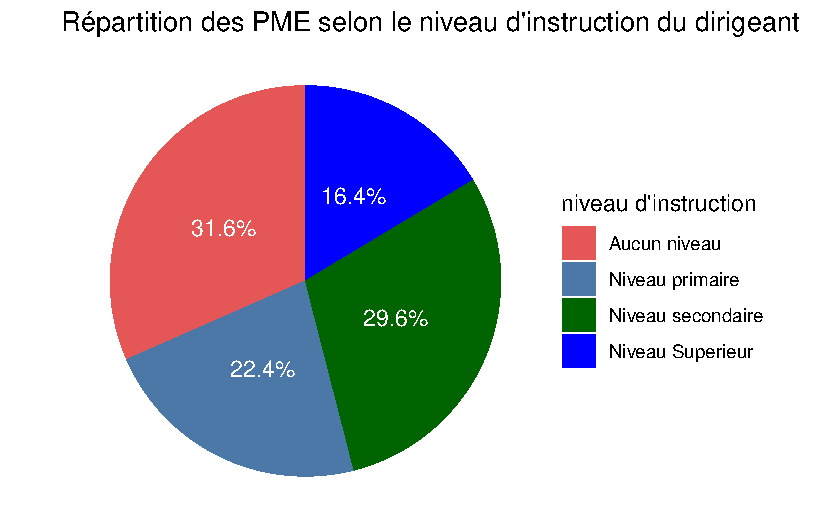
\includegraphics{projet_R_files/figure-pdf/unnamed-chunk-21-1.pdf}

}

\end{figure}

\begin{itemize}
\tightlist
\item
  Répartition des PME selon le statut juridique
\end{itemize}

\begin{Shaded}
\begin{Highlighting}[]
\CommentTok{\#q12}


\CommentTok{\# Répartition des PME selon le statut juridique}
\NormalTok{pme\_repartition }\OtherTok{\textless{}{-}}\NormalTok{ projet }\SpecialCharTok{\%\textgreater{}\%}
  \FunctionTok{select}\NormalTok{(q12) }\SpecialCharTok{\%\textgreater{}\%}
  \FunctionTok{count}\NormalTok{(q12) }\SpecialCharTok{\%\textgreater{}\%}
  \FunctionTok{mutate}\NormalTok{(}\AttributeTok{percentage =}\NormalTok{ n }\SpecialCharTok{/} \FunctionTok{sum}\NormalTok{(n) }\SpecialCharTok{*} \DecValTok{100}\NormalTok{)  }\CommentTok{\# Calcul du pourcentage}

\CommentTok{\# Création du diagramme en barres }

\FunctionTok{ggplot}\NormalTok{(pme\_repartition, }\FunctionTok{aes}\NormalTok{(}\AttributeTok{x =} \StringTok{""}\NormalTok{, }\AttributeTok{y =}\NormalTok{ n, }\AttributeTok{fill =}\NormalTok{ q12)) }\SpecialCharTok{+}
  \FunctionTok{geom\_bar}\NormalTok{(}\AttributeTok{stat =} \StringTok{"identity"}\NormalTok{) }\SpecialCharTok{+}
  \FunctionTok{scale\_fill\_manual}\NormalTok{(}\AttributeTok{values =} \FunctionTok{c}\NormalTok{(}\StringTok{"\#E45756"}\NormalTok{, }\StringTok{"\#4C78A8"}\NormalTok{,}\StringTok{"darkgreen"}\NormalTok{,}\StringTok{"blue"}\NormalTok{,}\StringTok{"pink"}\NormalTok{,}\StringTok{"lightgreen"}\NormalTok{)) }\SpecialCharTok{+}  \CommentTok{\# Couleurs des barres (à personnaliser)}
  \FunctionTok{labs}\NormalTok{(}\AttributeTok{x =} \ConstantTok{NULL}\NormalTok{, }\AttributeTok{y =} \ConstantTok{NULL}\NormalTok{, }\AttributeTok{fill =} \StringTok{"Statut juridique"}\NormalTok{) }\SpecialCharTok{+}
  \FunctionTok{geom\_text}\NormalTok{(}\FunctionTok{aes}\NormalTok{(}\AttributeTok{label =} \FunctionTok{paste0}\NormalTok{(}\FunctionTok{round}\NormalTok{(percentage, }\DecValTok{1}\NormalTok{), }\StringTok{"\%"}\NormalTok{)), }\AttributeTok{position =} \FunctionTok{position\_stack}\NormalTok{(}\AttributeTok{vjust =} \FloatTok{0.5}\NormalTok{), }\AttributeTok{color =} \StringTok{"white"}\NormalTok{) }\SpecialCharTok{+}
  \FunctionTok{theme\_minimal}\NormalTok{() }\SpecialCharTok{+}
  \FunctionTok{labs}\NormalTok{(}\AttributeTok{title =} \StringTok{"Répartition des PME selon le statut juridique"}\NormalTok{)}
\end{Highlighting}
\end{Shaded}

\begin{figure}[H]

{\centering 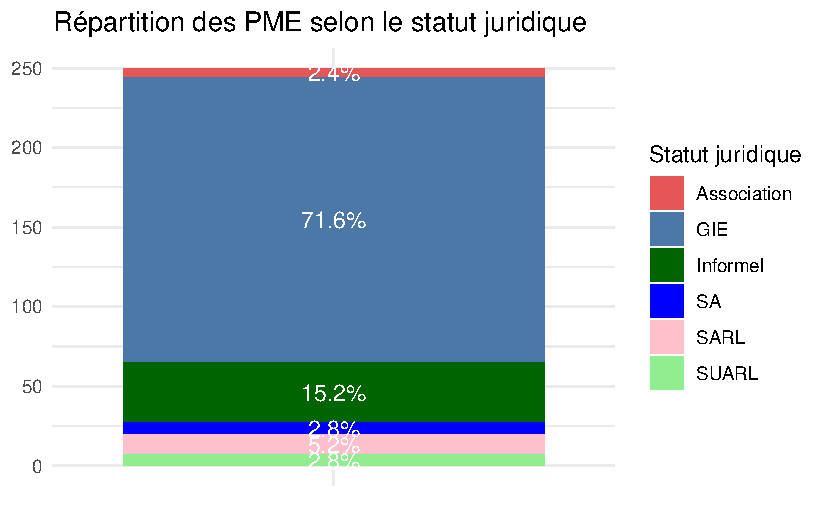
\includegraphics{projet_R_files/figure-pdf/unnamed-chunk-22-1.pdf}

}

\end{figure}

\begin{itemize}
\tightlist
\item
  Répartition des PME selon prop/locataire
\end{itemize}

\begin{Shaded}
\begin{Highlighting}[]
\CommentTok{\#Q81}


\CommentTok{\# Répartition des PME selon prop/locataire }
\NormalTok{pme\_repartition }\OtherTok{\textless{}{-}}\NormalTok{ projet }\SpecialCharTok{\%\textgreater{}\%}
  \FunctionTok{select}\NormalTok{(q81) }\SpecialCharTok{\%\textgreater{}\%}
  \FunctionTok{count}\NormalTok{(q81) }\SpecialCharTok{\%\textgreater{}\%}
  \FunctionTok{mutate}\NormalTok{(}\AttributeTok{percentage =}\NormalTok{ n }\SpecialCharTok{/} \FunctionTok{sum}\NormalTok{(n) }\SpecialCharTok{*} \DecValTok{100}\NormalTok{)  }\CommentTok{\# Calcul du pourcentage}

\CommentTok{\# Création du graphique en secteurs plein (pie chart) avec les pourcentages}

\FunctionTok{ggplot}\NormalTok{(pme\_repartition, }\FunctionTok{aes}\NormalTok{(}\AttributeTok{x =} \StringTok{""}\NormalTok{, }\AttributeTok{y =}\NormalTok{ n, }\AttributeTok{fill =}\NormalTok{ q81)) }\SpecialCharTok{+}
  \FunctionTok{geom\_bar}\NormalTok{(}\AttributeTok{stat =} \StringTok{"identity"}\NormalTok{, }\AttributeTok{position =} \StringTok{"fill"}\NormalTok{) }\SpecialCharTok{+}
  \FunctionTok{coord\_polar}\NormalTok{(}\StringTok{"y"}\NormalTok{) }\SpecialCharTok{+}
  \FunctionTok{scale\_fill\_manual}\NormalTok{(}\AttributeTok{values =} \FunctionTok{c}\NormalTok{(}\StringTok{"\#E45756"}\NormalTok{, }\StringTok{"\#4C78A8"}\NormalTok{)) }\SpecialCharTok{+}  \CommentTok{\# Couleurs des secteurs (à personnaliser)}
  \FunctionTok{labs}\NormalTok{(}\AttributeTok{x =} \ConstantTok{NULL}\NormalTok{, }\AttributeTok{y =} \ConstantTok{NULL}\NormalTok{, }\AttributeTok{fill =} \StringTok{"type du dirigeant"}\NormalTok{) }\SpecialCharTok{+}
  \FunctionTok{geom\_text}\NormalTok{(}\FunctionTok{aes}\NormalTok{(}\AttributeTok{label =} \FunctionTok{paste0}\NormalTok{(}\FunctionTok{round}\NormalTok{(percentage, }\DecValTok{1}\NormalTok{), }\StringTok{"\%"}\NormalTok{)), }\AttributeTok{position =} \FunctionTok{position\_fill}\NormalTok{(}\AttributeTok{vjust =} \FloatTok{0.5}\NormalTok{), }\AttributeTok{color =} \StringTok{"white"}\NormalTok{) }\SpecialCharTok{+}
  \FunctionTok{theme\_void}\NormalTok{()}\SpecialCharTok{+}
  \FunctionTok{labs}\NormalTok{(}\AttributeTok{title =} \StringTok{"Répartition des PME selon le type du dirigeant"}\NormalTok{)}
\end{Highlighting}
\end{Shaded}

\begin{figure}[H]

{\centering 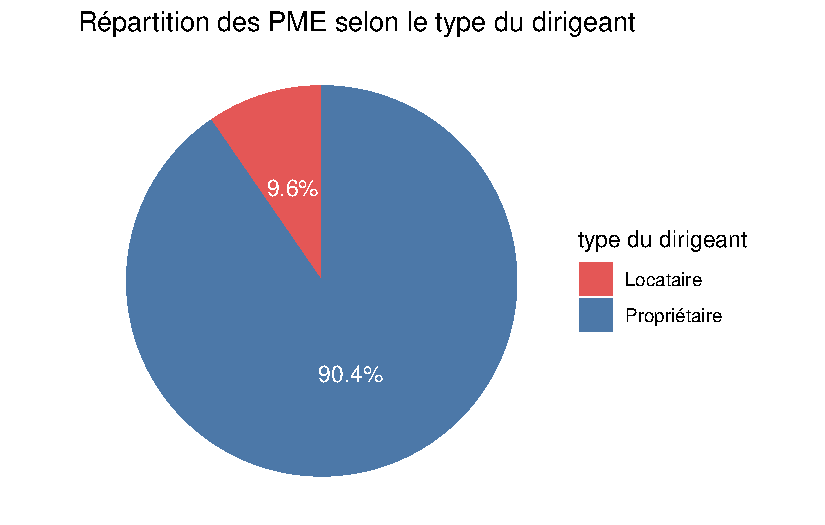
\includegraphics{projet_R_files/figure-pdf/unnamed-chunk-23-1.pdf}

}

\end{figure}

\hypertarget{statistiques-descriptives-bivariuxe9es}{%
\subsubsection{2.2 statistiques descriptives
bivariées}\label{statistiques-descriptives-bivariuxe9es}}

\hypertarget{tableaux-statistiques-1}{%
\paragraph{2.2.1. Tableaux statistiques}\label{tableaux-statistiques-1}}

\begin{itemize}
\item
  le statut juridique et le sexe
\item
  Niveau d'instruction du dirigeant/responsable de la PME et sexe
\item
  propriétaire ou locataire et sexe
\end{itemize}

\begin{Shaded}
\begin{Highlighting}[]
\CommentTok{\# Répartition selon le statut juridique et le sexe,Niveau d\textquotesingle{}instruction du dirigeant/responsable de la PME et sexe, propriétaire ou locataire et sexe : profil colonne}

\NormalTok{projet }\SpecialCharTok{\%\textgreater{}\%}
     \FunctionTok{select}\NormalTok{(q81,q25,q12, sexe) }\SpecialCharTok{\%\textgreater{}\%}
       \FunctionTok{rename}\NormalTok{(}\StringTok{"Niveau d’instruction du dirigeant/responsable de la PME"} \OtherTok{=}\NormalTok{ q25, }
         \StringTok{"Statut juridique*"}\OtherTok{=}\NormalTok{q12, }\StringTok{"propriétaire ou locataire"}\OtherTok{=}\NormalTok{q81) }\SpecialCharTok{\%\textgreater{}\%} 
            \FunctionTok{tbl\_summary}\NormalTok{(}\AttributeTok{by =}\NormalTok{ sexe, }\AttributeTok{missing =} \StringTok{"no"}\NormalTok{)}\SpecialCharTok{\%\textgreater{}\%}
              \FunctionTok{modify\_spanning\_header}\NormalTok{(}\FunctionTok{everything}\NormalTok{() }\SpecialCharTok{\textasciitilde{}} \StringTok{"**Répartition des PME selon leur statut juridique et le sexe de son dirigeant**"}\NormalTok{)}\SpecialCharTok{\%\textgreater{}\%} 
                   \FunctionTok{bold\_labels}\NormalTok{()}
\end{Highlighting}
\end{Shaded}

\begin{tabular}{l|c|c}
\hline
**Characteristic** & **Femme**, N = 191 & **Homme**, N = 59\\
\hline
\_\_propriétaire ou locataire\_\_ &  & \\
\hline
Locataire & 16 (8.4\%) & 8 (14\%)\\
\hline
Propriétaire & 175 (92\%) & 51 (86\%)\\
\hline
\_\_Niveau d’instruction du dirigeant/responsable de la PME\_\_ &  & \\
\hline
Aucun niveau & 70 (37\%) & 9 (15\%)\\
\hline
Niveau primaire & 48 (25\%) & 8 (14\%)\\
\hline
Niveau secondaire & 56 (29\%) & 18 (31\%)\\
\hline
Niveau Superieur & 17 (8.9\%) & 24 (41\%)\\
\hline
\_\_Statut juridique*\_\_ &  & \\
\hline
Association & 3 (1.6\%) & 3 (5.1\%)\\
\hline
GIE & 149 (78\%) & 30 (51\%)\\
\hline
Informel & 32 (17\%) & 6 (10\%)\\
\hline
SA & 1 (0.5\%) & 6 (10\%)\\
\hline
SARL & 2 (1.0\%) & 11 (19\%)\\
\hline
SUARL & 4 (2.1\%) & 3 (5.1\%)\\
\hline
\end{tabular}

\ul{\textbf{\emph{Commentaire:}}}\\
\strut \\

\hypertarget{activituxe9-principale-de-lentreprise-par-filiuxe8re}{%
\paragraph{2.2.2. Activité principale de l'entreprise par
filière}\label{activituxe9-principale-de-lentreprise-par-filiuxe8re}}

\begin{itemize}
\tightlist
\item
  Activite principale de l'entreprise par rapport au filière
\end{itemize}

\begin{Shaded}
\begin{Highlighting}[]
\CommentTok{\#}
\NormalTok{tab5}\OtherTok{=}\NormalTok{projet }\SpecialCharTok{\%\textgreater{}\%}
    \FunctionTok{select}\NormalTok{(q8, }\FunctionTok{starts\_with}\NormalTok{(}\StringTok{"filiere\_"}\NormalTok{)) }\SpecialCharTok{\%\textgreater{}\%}
      \FunctionTok{tbl\_summary}\NormalTok{(}\AttributeTok{by =}\NormalTok{ q8, }\AttributeTok{missing =} \StringTok{"no"}\NormalTok{)}\SpecialCharTok{\%\textgreater{}\%}
        \FunctionTok{modify\_spanning\_header}\NormalTok{(}\FunctionTok{everything}\NormalTok{() }\SpecialCharTok{\textasciitilde{}} \StringTok{"**Répartition des PME selon la filière et l\textquotesingle{}Activité principale de l’entreprise**"}\NormalTok{)}\SpecialCharTok{\%\textgreater{}\%} 
            \FunctionTok{bold\_labels}\NormalTok{()}



\NormalTok{tab5}\SpecialCharTok{\%\textgreater{}\%} \FunctionTok{bold\_labels}\NormalTok{() }\SpecialCharTok{\%\textgreater{}\%} 
  \FunctionTok{italicize\_levels}\NormalTok{()  }\SpecialCharTok{\%\textgreater{}\%} 
  \FunctionTok{modify\_header}\NormalTok{(}\AttributeTok{update =} \FunctionTok{list}\NormalTok{( label }\SpecialCharTok{\textasciitilde{}} \StringTok{"**VARIABLE**"}\NormalTok{, }\FunctionTok{all\_stat\_cols}\NormalTok{(}\AttributeTok{stat\_0 =} \ConstantTok{FALSE}\NormalTok{) }\SpecialCharTok{\textasciitilde{}} \StringTok{"**\{level\}** (n=\{n\}, \{style\_percent(p)\}\%)"}
\NormalTok{  )) }\SpecialCharTok{\%\textgreater{}\%}  \FunctionTok{as\_flex\_table}\NormalTok{() }\SpecialCharTok{\%\textgreater{}\%}
  \FunctionTok{fontsize}\NormalTok{(}\AttributeTok{size =} \DecValTok{8}\NormalTok{) }\SpecialCharTok{\%\textgreater{}\%}
  \FunctionTok{width}\NormalTok{(}\AttributeTok{width =} \FloatTok{1.65}\NormalTok{)}
\end{Highlighting}
\end{Shaded}

\global\setlength{\Oldarrayrulewidth}{\arrayrulewidth}

\global\setlength{\Oldtabcolsep}{\tabcolsep}

\setlength{\tabcolsep}{0pt}

\renewcommand*{\arraystretch}{1.5}



\providecommand{\ascline}[3]{\noalign{\global\arrayrulewidth #1}\arrayrulecolor[HTML]{#2}\cline{#3}}

\begin{longtable*}[c]{|p{1.65in}|p{1.65in}|p{1.65in}|p{1.65in}|p{1.65in}|p{1.65in}|p{1.65in}|p{1.65in}|p{1.65in}|p{1.65in}|p{1.65in}}



\ascline{1pt}{000000}{1-11}

\multicolumn{11}{>{\raggedright}m{\dimexpr 18.15in+20\tabcolsep}}{\textcolor[HTML]{000000}{\fontsize{11}{11}\selectfont{\textbf{Répartition\ des\ PME\ selon\ la\ filière\ et\ l'Activité\ principale\ de\ l’entreprise}}}} \\

\ascline{1pt}{000000}{1-11}



\multicolumn{1}{>{\raggedright}m{\dimexpr 1.65in+0\tabcolsep}}{\textcolor[HTML]{000000}{\fontsize{11}{11}\selectfont{\textbf{VARIABLE}}}} & \multicolumn{1}{>{\centering}m{\dimexpr 1.65in+0\tabcolsep}}{\textcolor[HTML]{000000}{\fontsize{11}{11}\selectfont{\textbf{Aucun}}}\textcolor[HTML]{000000}{\fontsize{11}{11}\selectfont{\ (n=5,\ 2.0\%)}}\textcolor[HTML]{000000}{\textsuperscript{\fontsize{11}{11}\selectfont{1}}}} & \multicolumn{1}{>{\centering}m{\dimexpr 1.65in+0\tabcolsep}}{\textcolor[HTML]{000000}{\fontsize{11}{11}\selectfont{\textbf{Autre\ a\ preciser}}}\textcolor[HTML]{000000}{\fontsize{11}{11}\selectfont{\ (n=4,\ 1.6\%)}}\textcolor[HTML]{000000}{\textsuperscript{\fontsize{11}{11}\selectfont{1}}}} & \multicolumn{1}{>{\centering}m{\dimexpr 1.65in+0\tabcolsep}}{\textcolor[HTML]{000000}{\fontsize{11}{11}\selectfont{\textbf{Tansformation\ d'autres\ céréales}}}\textcolor[HTML]{000000}{\fontsize{11}{11}\selectfont{\ (n=57,\ 23\%)}}\textcolor[HTML]{000000}{\textsuperscript{\fontsize{11}{11}\selectfont{1}}}} & \multicolumn{1}{>{\centering}m{\dimexpr 1.65in+0\tabcolsep}}{\textcolor[HTML]{000000}{\fontsize{11}{11}\selectfont{\textbf{Transformation\ d'autres\ fruits\ et\ legumes}}}\textcolor[HTML]{000000}{\fontsize{11}{11}\selectfont{\ (n=14,\ 5.6\%)}}\textcolor[HTML]{000000}{\textsuperscript{\fontsize{11}{11}\selectfont{1}}}} & \multicolumn{1}{>{\centering}m{\dimexpr 1.65in+0\tabcolsep}}{\textcolor[HTML]{000000}{\fontsize{11}{11}\selectfont{\textbf{Transformation\ d'autres\ produits\ oléagineux}}}\textcolor[HTML]{000000}{\fontsize{11}{11}\selectfont{\ (n=1,\ 0.4\%)}}\textcolor[HTML]{000000}{\textsuperscript{\fontsize{11}{11}\selectfont{1}}}} & \multicolumn{1}{>{\centering}m{\dimexpr 1.65in+0\tabcolsep}}{\textcolor[HTML]{000000}{\fontsize{11}{11}\selectfont{\textbf{Transformation\ de\ l'arachide}}}\textcolor[HTML]{000000}{\fontsize{11}{11}\selectfont{\ (n=47,\ 19\%)}}\textcolor[HTML]{000000}{\textsuperscript{\fontsize{11}{11}\selectfont{1}}}} & \multicolumn{1}{>{\centering}m{\dimexpr 1.65in+0\tabcolsep}}{\textcolor[HTML]{000000}{\fontsize{11}{11}\selectfont{\textbf{Transformation\ de\ la\ mangue}}}\textcolor[HTML]{000000}{\fontsize{11}{11}\selectfont{\ (n=35,\ 14\%)}}\textcolor[HTML]{000000}{\textsuperscript{\fontsize{11}{11}\selectfont{1}}}} & \multicolumn{1}{>{\centering}m{\dimexpr 1.65in+0\tabcolsep}}{\textcolor[HTML]{000000}{\fontsize{11}{11}\selectfont{\textbf{Transformation\ de\ la\ noix\ de\ cajoux}}}\textcolor[HTML]{000000}{\fontsize{11}{11}\selectfont{\ (n=32,\ 13\%)}}\textcolor[HTML]{000000}{\textsuperscript{\fontsize{11}{11}\selectfont{1}}}} & \multicolumn{1}{>{\centering}m{\dimexpr 1.65in+0\tabcolsep}}{\textcolor[HTML]{000000}{\fontsize{11}{11}\selectfont{\textbf{Transformation\ de\ la\ pomme\ de\ cajoux}}}\textcolor[HTML]{000000}{\fontsize{11}{11}\selectfont{\ (n=9,\ 3.6\%)}}\textcolor[HTML]{000000}{\textsuperscript{\fontsize{11}{11}\selectfont{1}}}} & \multicolumn{1}{>{\centering}m{\dimexpr 1.65in+0\tabcolsep}}{\textcolor[HTML]{000000}{\fontsize{11}{11}\selectfont{\textbf{Transformation\ du\ riz}}}\textcolor[HTML]{000000}{\fontsize{11}{11}\selectfont{\ (n=46,\ 18\%)}}\textcolor[HTML]{000000}{\textsuperscript{\fontsize{11}{11}\selectfont{1}}}} \\

\ascline{1pt}{000000}{1-11}\endfirsthead 

\ascline{1pt}{000000}{1-11}

\multicolumn{11}{>{\raggedright}m{\dimexpr 18.15in+20\tabcolsep}}{\textcolor[HTML]{000000}{\fontsize{11}{11}\selectfont{\textbf{Répartition\ des\ PME\ selon\ la\ filière\ et\ l'Activité\ principale\ de\ l’entreprise}}}} \\

\ascline{1pt}{000000}{1-11}



\multicolumn{1}{>{\raggedright}m{\dimexpr 1.65in+0\tabcolsep}}{\textcolor[HTML]{000000}{\fontsize{11}{11}\selectfont{\textbf{VARIABLE}}}} & \multicolumn{1}{>{\centering}m{\dimexpr 1.65in+0\tabcolsep}}{\textcolor[HTML]{000000}{\fontsize{11}{11}\selectfont{\textbf{Aucun}}}\textcolor[HTML]{000000}{\fontsize{11}{11}\selectfont{\ (n=5,\ 2.0\%)}}\textcolor[HTML]{000000}{\textsuperscript{\fontsize{11}{11}\selectfont{1}}}} & \multicolumn{1}{>{\centering}m{\dimexpr 1.65in+0\tabcolsep}}{\textcolor[HTML]{000000}{\fontsize{11}{11}\selectfont{\textbf{Autre\ a\ preciser}}}\textcolor[HTML]{000000}{\fontsize{11}{11}\selectfont{\ (n=4,\ 1.6\%)}}\textcolor[HTML]{000000}{\textsuperscript{\fontsize{11}{11}\selectfont{1}}}} & \multicolumn{1}{>{\centering}m{\dimexpr 1.65in+0\tabcolsep}}{\textcolor[HTML]{000000}{\fontsize{11}{11}\selectfont{\textbf{Tansformation\ d'autres\ céréales}}}\textcolor[HTML]{000000}{\fontsize{11}{11}\selectfont{\ (n=57,\ 23\%)}}\textcolor[HTML]{000000}{\textsuperscript{\fontsize{11}{11}\selectfont{1}}}} & \multicolumn{1}{>{\centering}m{\dimexpr 1.65in+0\tabcolsep}}{\textcolor[HTML]{000000}{\fontsize{11}{11}\selectfont{\textbf{Transformation\ d'autres\ fruits\ et\ legumes}}}\textcolor[HTML]{000000}{\fontsize{11}{11}\selectfont{\ (n=14,\ 5.6\%)}}\textcolor[HTML]{000000}{\textsuperscript{\fontsize{11}{11}\selectfont{1}}}} & \multicolumn{1}{>{\centering}m{\dimexpr 1.65in+0\tabcolsep}}{\textcolor[HTML]{000000}{\fontsize{11}{11}\selectfont{\textbf{Transformation\ d'autres\ produits\ oléagineux}}}\textcolor[HTML]{000000}{\fontsize{11}{11}\selectfont{\ (n=1,\ 0.4\%)}}\textcolor[HTML]{000000}{\textsuperscript{\fontsize{11}{11}\selectfont{1}}}} & \multicolumn{1}{>{\centering}m{\dimexpr 1.65in+0\tabcolsep}}{\textcolor[HTML]{000000}{\fontsize{11}{11}\selectfont{\textbf{Transformation\ de\ l'arachide}}}\textcolor[HTML]{000000}{\fontsize{11}{11}\selectfont{\ (n=47,\ 19\%)}}\textcolor[HTML]{000000}{\textsuperscript{\fontsize{11}{11}\selectfont{1}}}} & \multicolumn{1}{>{\centering}m{\dimexpr 1.65in+0\tabcolsep}}{\textcolor[HTML]{000000}{\fontsize{11}{11}\selectfont{\textbf{Transformation\ de\ la\ mangue}}}\textcolor[HTML]{000000}{\fontsize{11}{11}\selectfont{\ (n=35,\ 14\%)}}\textcolor[HTML]{000000}{\textsuperscript{\fontsize{11}{11}\selectfont{1}}}} & \multicolumn{1}{>{\centering}m{\dimexpr 1.65in+0\tabcolsep}}{\textcolor[HTML]{000000}{\fontsize{11}{11}\selectfont{\textbf{Transformation\ de\ la\ noix\ de\ cajoux}}}\textcolor[HTML]{000000}{\fontsize{11}{11}\selectfont{\ (n=32,\ 13\%)}}\textcolor[HTML]{000000}{\textsuperscript{\fontsize{11}{11}\selectfont{1}}}} & \multicolumn{1}{>{\centering}m{\dimexpr 1.65in+0\tabcolsep}}{\textcolor[HTML]{000000}{\fontsize{11}{11}\selectfont{\textbf{Transformation\ de\ la\ pomme\ de\ cajoux}}}\textcolor[HTML]{000000}{\fontsize{11}{11}\selectfont{\ (n=9,\ 3.6\%)}}\textcolor[HTML]{000000}{\textsuperscript{\fontsize{11}{11}\selectfont{1}}}} & \multicolumn{1}{>{\centering}m{\dimexpr 1.65in+0\tabcolsep}}{\textcolor[HTML]{000000}{\fontsize{11}{11}\selectfont{\textbf{Transformation\ du\ riz}}}\textcolor[HTML]{000000}{\fontsize{11}{11}\selectfont{\ (n=46,\ 18\%)}}\textcolor[HTML]{000000}{\textsuperscript{\fontsize{11}{11}\selectfont{1}}}} \\

\ascline{1pt}{000000}{1-11}\endhead



\multicolumn{1}{>{\raggedright}p{\dimexpr 1.65in+0\tabcolsep}}{\textcolor[HTML]{000000}{\fontsize{8}{8}\selectfont{\textbf{filiere\_1}}}} & \multicolumn{1}{>{\centering}p{\dimexpr 1.65in+0\tabcolsep}}{\textcolor[HTML]{000000}{\fontsize{8}{8}\selectfont{5\ (100\%)}}} & \multicolumn{1}{>{\centering}p{\dimexpr 1.65in+0\tabcolsep}}{\textcolor[HTML]{000000}{\fontsize{8}{8}\selectfont{1\ (25\%)}}} & \multicolumn{1}{>{\centering}p{\dimexpr 1.65in+0\tabcolsep}}{\textcolor[HTML]{000000}{\fontsize{8}{8}\selectfont{38\ (67\%)}}} & \multicolumn{1}{>{\centering}p{\dimexpr 1.65in+0\tabcolsep}}{\textcolor[HTML]{000000}{\fontsize{8}{8}\selectfont{7\ (50\%)}}} & \multicolumn{1}{>{\centering}p{\dimexpr 1.65in+0\tabcolsep}}{\textcolor[HTML]{000000}{\fontsize{8}{8}\selectfont{1\ (100\%)}}} & \multicolumn{1}{>{\centering}p{\dimexpr 1.65in+0\tabcolsep}}{\textcolor[HTML]{000000}{\fontsize{8}{8}\selectfont{47\ (100\%)}}} & \multicolumn{1}{>{\centering}p{\dimexpr 1.65in+0\tabcolsep}}{\textcolor[HTML]{000000}{\fontsize{8}{8}\selectfont{3\ (8.6\%)}}} & \multicolumn{1}{>{\centering}p{\dimexpr 1.65in+0\tabcolsep}}{\textcolor[HTML]{000000}{\fontsize{8}{8}\selectfont{3\ (9.4\%)}}} & \multicolumn{1}{>{\centering}p{\dimexpr 1.65in+0\tabcolsep}}{\textcolor[HTML]{000000}{\fontsize{8}{8}\selectfont{1\ (11\%)}}} & \multicolumn{1}{>{\centering}p{\dimexpr 1.65in+0\tabcolsep}}{\textcolor[HTML]{000000}{\fontsize{8}{8}\selectfont{2\ (4.3\%)}}} \\





\multicolumn{1}{>{\raggedright}p{\dimexpr 1.65in+0\tabcolsep}}{\textcolor[HTML]{000000}{\fontsize{8}{8}\selectfont{\textbf{filiere\_2}}}} & \multicolumn{1}{>{\centering}p{\dimexpr 1.65in+0\tabcolsep}}{\textcolor[HTML]{000000}{\fontsize{8}{8}\selectfont{0\ (0\%)}}} & \multicolumn{1}{>{\centering}p{\dimexpr 1.65in+0\tabcolsep}}{\textcolor[HTML]{000000}{\fontsize{8}{8}\selectfont{0\ (0\%)}}} & \multicolumn{1}{>{\centering}p{\dimexpr 1.65in+0\tabcolsep}}{\textcolor[HTML]{000000}{\fontsize{8}{8}\selectfont{1\ (1.8\%)}}} & \multicolumn{1}{>{\centering}p{\dimexpr 1.65in+0\tabcolsep}}{\textcolor[HTML]{000000}{\fontsize{8}{8}\selectfont{2\ (14\%)}}} & \multicolumn{1}{>{\centering}p{\dimexpr 1.65in+0\tabcolsep}}{\textcolor[HTML]{000000}{\fontsize{8}{8}\selectfont{0\ (0\%)}}} & \multicolumn{1}{>{\centering}p{\dimexpr 1.65in+0\tabcolsep}}{\textcolor[HTML]{000000}{\fontsize{8}{8}\selectfont{4\ (8.5\%)}}} & \multicolumn{1}{>{\centering}p{\dimexpr 1.65in+0\tabcolsep}}{\textcolor[HTML]{000000}{\fontsize{8}{8}\selectfont{13\ (37\%)}}} & \multicolumn{1}{>{\centering}p{\dimexpr 1.65in+0\tabcolsep}}{\textcolor[HTML]{000000}{\fontsize{8}{8}\selectfont{32\ (100\%)}}} & \multicolumn{1}{>{\centering}p{\dimexpr 1.65in+0\tabcolsep}}{\textcolor[HTML]{000000}{\fontsize{8}{8}\selectfont{9\ (100\%)}}} & \multicolumn{1}{>{\centering}p{\dimexpr 1.65in+0\tabcolsep}}{\textcolor[HTML]{000000}{\fontsize{8}{8}\selectfont{0\ (0\%)}}} \\





\multicolumn{1}{>{\raggedright}p{\dimexpr 1.65in+0\tabcolsep}}{\textcolor[HTML]{000000}{\fontsize{8}{8}\selectfont{\textbf{filiere\_3}}}} & \multicolumn{1}{>{\centering}p{\dimexpr 1.65in+0\tabcolsep}}{\textcolor[HTML]{000000}{\fontsize{8}{8}\selectfont{0\ (0\%)}}} & \multicolumn{1}{>{\centering}p{\dimexpr 1.65in+0\tabcolsep}}{\textcolor[HTML]{000000}{\fontsize{8}{8}\selectfont{0\ (0\%)}}} & \multicolumn{1}{>{\centering}p{\dimexpr 1.65in+0\tabcolsep}}{\textcolor[HTML]{000000}{\fontsize{8}{8}\selectfont{28\ (49\%)}}} & \multicolumn{1}{>{\centering}p{\dimexpr 1.65in+0\tabcolsep}}{\textcolor[HTML]{000000}{\fontsize{8}{8}\selectfont{6\ (43\%)}}} & \multicolumn{1}{>{\centering}p{\dimexpr 1.65in+0\tabcolsep}}{\textcolor[HTML]{000000}{\fontsize{8}{8}\selectfont{0\ (0\%)}}} & \multicolumn{1}{>{\centering}p{\dimexpr 1.65in+0\tabcolsep}}{\textcolor[HTML]{000000}{\fontsize{8}{8}\selectfont{4\ (8.5\%)}}} & \multicolumn{1}{>{\centering}p{\dimexpr 1.65in+0\tabcolsep}}{\textcolor[HTML]{000000}{\fontsize{8}{8}\selectfont{2\ (5.7\%)}}} & \multicolumn{1}{>{\centering}p{\dimexpr 1.65in+0\tabcolsep}}{\textcolor[HTML]{000000}{\fontsize{8}{8}\selectfont{0\ (0\%)}}} & \multicolumn{1}{>{\centering}p{\dimexpr 1.65in+0\tabcolsep}}{\textcolor[HTML]{000000}{\fontsize{8}{8}\selectfont{3\ (33\%)}}} & \multicolumn{1}{>{\centering}p{\dimexpr 1.65in+0\tabcolsep}}{\textcolor[HTML]{000000}{\fontsize{8}{8}\selectfont{46\ (100\%)}}} \\





\multicolumn{1}{>{\raggedright}p{\dimexpr 1.65in+0\tabcolsep}}{\textcolor[HTML]{000000}{\fontsize{8}{8}\selectfont{\textbf{filiere\_4}}}} & \multicolumn{1}{>{\centering}p{\dimexpr 1.65in+0\tabcolsep}}{\textcolor[HTML]{000000}{\fontsize{8}{8}\selectfont{0\ (0\%)}}} & \multicolumn{1}{>{\centering}p{\dimexpr 1.65in+0\tabcolsep}}{\textcolor[HTML]{000000}{\fontsize{8}{8}\selectfont{3\ (75\%)}}} & \multicolumn{1}{>{\centering}p{\dimexpr 1.65in+0\tabcolsep}}{\textcolor[HTML]{000000}{\fontsize{8}{8}\selectfont{21\ (37\%)}}} & \multicolumn{1}{>{\centering}p{\dimexpr 1.65in+0\tabcolsep}}{\textcolor[HTML]{000000}{\fontsize{8}{8}\selectfont{9\ (64\%)}}} & \multicolumn{1}{>{\centering}p{\dimexpr 1.65in+0\tabcolsep}}{\textcolor[HTML]{000000}{\fontsize{8}{8}\selectfont{0\ (0\%)}}} & \multicolumn{1}{>{\centering}p{\dimexpr 1.65in+0\tabcolsep}}{\textcolor[HTML]{000000}{\fontsize{8}{8}\selectfont{4\ (8.5\%)}}} & \multicolumn{1}{>{\centering}p{\dimexpr 1.65in+0\tabcolsep}}{\textcolor[HTML]{000000}{\fontsize{8}{8}\selectfont{35\ (100\%)}}} & \multicolumn{1}{>{\centering}p{\dimexpr 1.65in+0\tabcolsep}}{\textcolor[HTML]{000000}{\fontsize{8}{8}\selectfont{7\ (22\%)}}} & \multicolumn{1}{>{\centering}p{\dimexpr 1.65in+0\tabcolsep}}{\textcolor[HTML]{000000}{\fontsize{8}{8}\selectfont{9\ (100\%)}}} & \multicolumn{1}{>{\centering}p{\dimexpr 1.65in+0\tabcolsep}}{\textcolor[HTML]{000000}{\fontsize{8}{8}\selectfont{4\ (8.7\%)}}} \\

\ascline{1pt}{000000}{1-11}



\multicolumn{11}{>{\raggedright}m{\dimexpr 18.15in+20\tabcolsep}}{\textcolor[HTML]{000000}{\textsuperscript{\fontsize{11}{11}\selectfont{1}}}\textcolor[HTML]{000000}{\fontsize{11}{11}\selectfont{n\ (\%)}}} \\





\end{longtable*}



\arrayrulecolor[HTML]{000000}

\global\setlength{\arrayrulewidth}{\Oldarrayrulewidth}

\global\setlength{\tabcolsep}{\Oldtabcolsep}

\renewcommand*{\arraystretch}{1}

\begin{itemize}
\tightlist
\item
  Activité principale suivant les spécificités des filières
\end{itemize}

\begin{Shaded}
\begin{Highlighting}[]
\CommentTok{\#plus spécifiquement}
\NormalTok{tab6}\OtherTok{=}\NormalTok{projet }\SpecialCharTok{\%\textgreater{}\%}
  \FunctionTok{select}\NormalTok{(q8, nom\_filiere) }\SpecialCharTok{\%\textgreater{}\%}
     \FunctionTok{rename}\NormalTok{(}\StringTok{"Activité principale"}\OtherTok{=}\NormalTok{q8) }\SpecialCharTok{\%\textgreater{}\%} 
       \FunctionTok{tbl\_summary}\NormalTok{(}\AttributeTok{by =}\NormalTok{ nom\_filiere, }\AttributeTok{missing =} \StringTok{"no"}\NormalTok{)}\SpecialCharTok{\%\textgreater{}\%}
       \FunctionTok{modify\_spanning\_header}\NormalTok{(}\FunctionTok{everything}\NormalTok{() }\SpecialCharTok{\textasciitilde{}} \StringTok{"**Répartition des PME selon la filière et l\textquotesingle{}Activité principale de l’entreprise**"}\NormalTok{)}\SpecialCharTok{\%\textgreater{}\%} 
          \FunctionTok{bold\_labels}\NormalTok{()}


\NormalTok{tab6}\SpecialCharTok{\%\textgreater{}\%} \FunctionTok{bold\_labels}\NormalTok{() }\SpecialCharTok{\%\textgreater{}\%} 
  \FunctionTok{italicize\_levels}\NormalTok{()  }\SpecialCharTok{\%\textgreater{}\%} 
  \FunctionTok{modify\_header}\NormalTok{(}\AttributeTok{update =} \FunctionTok{list}\NormalTok{( label }\SpecialCharTok{\textasciitilde{}} \StringTok{"**VARIABLE**"}\NormalTok{, }\FunctionTok{all\_stat\_cols}\NormalTok{(}\AttributeTok{stat\_0 =} \ConstantTok{FALSE}\NormalTok{) }\SpecialCharTok{\textasciitilde{}} \StringTok{"**\{level\}** (n=\{n\}, \{style\_percent(p)\}\%)"}
\NormalTok{  )) }\SpecialCharTok{\%\textgreater{}\%}  \FunctionTok{as\_flex\_table}\NormalTok{() }\SpecialCharTok{\%\textgreater{}\%}
  \FunctionTok{fontsize}\NormalTok{(}\AttributeTok{size =} \DecValTok{8}\NormalTok{) }\SpecialCharTok{\%\textgreater{}\%}
  \FunctionTok{width}\NormalTok{(}\AttributeTok{width =} \FloatTok{1.65}\NormalTok{)}
\end{Highlighting}
\end{Shaded}

\global\setlength{\Oldarrayrulewidth}{\arrayrulewidth}

\global\setlength{\Oldtabcolsep}{\tabcolsep}

\setlength{\tabcolsep}{0pt}

\renewcommand*{\arraystretch}{1.5}



\providecommand{\ascline}[3]{\noalign{\global\arrayrulewidth #1}\arrayrulecolor[HTML]{#2}\cline{#3}}

\begin{longtable*}[c]{|p{1.65in}|p{1.65in}|p{1.65in}|p{1.65in}|p{1.65in}|p{1.65in}|p{1.65in}|p{1.65in}|p{1.65in}|p{1.65in}|p{1.65in}|p{1.65in}|p{1.65in}|p{1.65in}|p{1.65in}}



\ascline{1pt}{000000}{1-15}

\multicolumn{15}{>{\raggedright}m{\dimexpr 24.75in+28\tabcolsep}}{\textcolor[HTML]{000000}{\fontsize{11}{11}\selectfont{\textbf{Répartition\ des\ PME\ selon\ la\ filière\ et\ l'Activité\ principale\ de\ l’entreprise}}}} \\

\ascline{1pt}{000000}{1-15}



\multicolumn{1}{>{\raggedright}m{\dimexpr 1.65in+0\tabcolsep}}{\textcolor[HTML]{000000}{\fontsize{11}{11}\selectfont{\textbf{VARIABLE}}}} & \multicolumn{1}{>{\centering}m{\dimexpr 1.65in+0\tabcolsep}}{\textcolor[HTML]{000000}{\fontsize{11}{11}\selectfont{\textbf{anacarde}}}\textcolor[HTML]{000000}{\fontsize{11}{11}\selectfont{\ (n=25,\ 10\%)}}\textcolor[HTML]{000000}{\textsuperscript{\fontsize{11}{11}\selectfont{1}}}} & \multicolumn{1}{>{\centering}m{\dimexpr 1.65in+0\tabcolsep}}{\textcolor[HTML]{000000}{\fontsize{11}{11}\selectfont{\textbf{arachide}}}\textcolor[HTML]{000000}{\fontsize{11}{11}\selectfont{\ (n=61,\ 24\%)}}\textcolor[HTML]{000000}{\textsuperscript{\fontsize{11}{11}\selectfont{1}}}} & \multicolumn{1}{>{\centering}m{\dimexpr 1.65in+0\tabcolsep}}{\textcolor[HTML]{000000}{\fontsize{11}{11}\selectfont{\textbf{arachide\ \&\ anacarde}}}\textcolor[HTML]{000000}{\fontsize{11}{11}\selectfont{\ (n=6,\ 2.4\%)}}\textcolor[HTML]{000000}{\textsuperscript{\fontsize{11}{11}\selectfont{1}}}} & \multicolumn{1}{>{\centering}m{\dimexpr 1.65in+0\tabcolsep}}{\textcolor[HTML]{000000}{\fontsize{11}{11}\selectfont{\textbf{arachide\ \&\ anacarde\ \&\ mangue}}}\textcolor[HTML]{000000}{\fontsize{11}{11}\selectfont{\ (n=1,\ 0.4\%)}}\textcolor[HTML]{000000}{\textsuperscript{\fontsize{11}{11}\selectfont{1}}}} & \multicolumn{1}{>{\centering}m{\dimexpr 1.65in+0\tabcolsep}}{\textcolor[HTML]{000000}{\fontsize{11}{11}\selectfont{\textbf{arachide\ \&\ anacarde\ \&\ mangue\&\ riz}}}\textcolor[HTML]{000000}{\fontsize{11}{11}\selectfont{\ (n=1,\ 0.4\%)}}\textcolor[HTML]{000000}{\textsuperscript{\fontsize{11}{11}\selectfont{1}}}} & \multicolumn{1}{>{\centering}m{\dimexpr 1.65in+0\tabcolsep}}{\textcolor[HTML]{000000}{\fontsize{11}{11}\selectfont{\textbf{arachide\ \&\ anacarde\ \&\ riz}}}\textcolor[HTML]{000000}{\fontsize{11}{11}\selectfont{\ (n=2,\ 0.8\%)}}\textcolor[HTML]{000000}{\textsuperscript{\fontsize{11}{11}\selectfont{1}}}} & \multicolumn{1}{>{\centering}m{\dimexpr 1.65in+0\tabcolsep}}{\textcolor[HTML]{000000}{\fontsize{11}{11}\selectfont{\textbf{arachide\ \&\ mangue}}}\textcolor[HTML]{000000}{\fontsize{11}{11}\selectfont{\ (n=13,\ 5.2\%)}}\textcolor[HTML]{000000}{\textsuperscript{\fontsize{11}{11}\selectfont{1}}}} & \multicolumn{1}{>{\centering}m{\dimexpr 1.65in+0\tabcolsep}}{\textcolor[HTML]{000000}{\fontsize{11}{11}\selectfont{\textbf{arachide\ \&\ riz}}}\textcolor[HTML]{000000}{\fontsize{11}{11}\selectfont{\ (n=11,\ 4.4\%)}}\textcolor[HTML]{000000}{\textsuperscript{\fontsize{11}{11}\selectfont{1}}}} & \multicolumn{1}{>{\centering}m{\dimexpr 1.65in+0\tabcolsep}}{\textcolor[HTML]{000000}{\fontsize{11}{11}\selectfont{\textbf{arachide\ \&\ riz\ \&\ mangue}}}\textcolor[HTML]{000000}{\fontsize{11}{11}\selectfont{\ (n=13,\ 5.2\%)}}\textcolor[HTML]{000000}{\textsuperscript{\fontsize{11}{11}\selectfont{1}}}} & \multicolumn{1}{>{\centering}m{\dimexpr 1.65in+0\tabcolsep}}{\textcolor[HTML]{000000}{\fontsize{11}{11}\selectfont{\textbf{mangue}}}\textcolor[HTML]{000000}{\fontsize{11}{11}\selectfont{\ (n=52,\ 21\%)}}\textcolor[HTML]{000000}{\textsuperscript{\fontsize{11}{11}\selectfont{1}}}} & \multicolumn{1}{>{\centering}m{\dimexpr 1.65in+0\tabcolsep}}{\textcolor[HTML]{000000}{\fontsize{11}{11}\selectfont{\textbf{riz}}}\textcolor[HTML]{000000}{\fontsize{11}{11}\selectfont{\ (n=33,\ 13\%)}}\textcolor[HTML]{000000}{\textsuperscript{\fontsize{11}{11}\selectfont{1}}}} & \multicolumn{1}{>{\centering}m{\dimexpr 1.65in+0\tabcolsep}}{\textcolor[HTML]{000000}{\fontsize{11}{11}\selectfont{\textbf{riz\ \&\ anacarde}}}\textcolor[HTML]{000000}{\fontsize{11}{11}\selectfont{\ (n=23,\ 9.2\%)}}\textcolor[HTML]{000000}{\textsuperscript{\fontsize{11}{11}\selectfont{1}}}} & \multicolumn{1}{>{\centering}m{\dimexpr 1.65in+0\tabcolsep}}{\textcolor[HTML]{000000}{\fontsize{11}{11}\selectfont{\textbf{riz\ \&\ anacarde\ \&\ mangue}}}\textcolor[HTML]{000000}{\fontsize{11}{11}\selectfont{\ (n=3,\ 1.2\%)}}\textcolor[HTML]{000000}{\textsuperscript{\fontsize{11}{11}\selectfont{1}}}} & \multicolumn{1}{>{\centering}m{\dimexpr 1.65in+0\tabcolsep}}{\textcolor[HTML]{000000}{\fontsize{11}{11}\selectfont{\textbf{riz\ \&\ mangue}}}\textcolor[HTML]{000000}{\fontsize{11}{11}\selectfont{\ (n=6,\ 2.4\%)}}\textcolor[HTML]{000000}{\textsuperscript{\fontsize{11}{11}\selectfont{1}}}} \\

\ascline{1pt}{000000}{1-15}\endfirsthead 

\ascline{1pt}{000000}{1-15}

\multicolumn{15}{>{\raggedright}m{\dimexpr 24.75in+28\tabcolsep}}{\textcolor[HTML]{000000}{\fontsize{11}{11}\selectfont{\textbf{Répartition\ des\ PME\ selon\ la\ filière\ et\ l'Activité\ principale\ de\ l’entreprise}}}} \\

\ascline{1pt}{000000}{1-15}



\multicolumn{1}{>{\raggedright}m{\dimexpr 1.65in+0\tabcolsep}}{\textcolor[HTML]{000000}{\fontsize{11}{11}\selectfont{\textbf{VARIABLE}}}} & \multicolumn{1}{>{\centering}m{\dimexpr 1.65in+0\tabcolsep}}{\textcolor[HTML]{000000}{\fontsize{11}{11}\selectfont{\textbf{anacarde}}}\textcolor[HTML]{000000}{\fontsize{11}{11}\selectfont{\ (n=25,\ 10\%)}}\textcolor[HTML]{000000}{\textsuperscript{\fontsize{11}{11}\selectfont{1}}}} & \multicolumn{1}{>{\centering}m{\dimexpr 1.65in+0\tabcolsep}}{\textcolor[HTML]{000000}{\fontsize{11}{11}\selectfont{\textbf{arachide}}}\textcolor[HTML]{000000}{\fontsize{11}{11}\selectfont{\ (n=61,\ 24\%)}}\textcolor[HTML]{000000}{\textsuperscript{\fontsize{11}{11}\selectfont{1}}}} & \multicolumn{1}{>{\centering}m{\dimexpr 1.65in+0\tabcolsep}}{\textcolor[HTML]{000000}{\fontsize{11}{11}\selectfont{\textbf{arachide\ \&\ anacarde}}}\textcolor[HTML]{000000}{\fontsize{11}{11}\selectfont{\ (n=6,\ 2.4\%)}}\textcolor[HTML]{000000}{\textsuperscript{\fontsize{11}{11}\selectfont{1}}}} & \multicolumn{1}{>{\centering}m{\dimexpr 1.65in+0\tabcolsep}}{\textcolor[HTML]{000000}{\fontsize{11}{11}\selectfont{\textbf{arachide\ \&\ anacarde\ \&\ mangue}}}\textcolor[HTML]{000000}{\fontsize{11}{11}\selectfont{\ (n=1,\ 0.4\%)}}\textcolor[HTML]{000000}{\textsuperscript{\fontsize{11}{11}\selectfont{1}}}} & \multicolumn{1}{>{\centering}m{\dimexpr 1.65in+0\tabcolsep}}{\textcolor[HTML]{000000}{\fontsize{11}{11}\selectfont{\textbf{arachide\ \&\ anacarde\ \&\ mangue\&\ riz}}}\textcolor[HTML]{000000}{\fontsize{11}{11}\selectfont{\ (n=1,\ 0.4\%)}}\textcolor[HTML]{000000}{\textsuperscript{\fontsize{11}{11}\selectfont{1}}}} & \multicolumn{1}{>{\centering}m{\dimexpr 1.65in+0\tabcolsep}}{\textcolor[HTML]{000000}{\fontsize{11}{11}\selectfont{\textbf{arachide\ \&\ anacarde\ \&\ riz}}}\textcolor[HTML]{000000}{\fontsize{11}{11}\selectfont{\ (n=2,\ 0.8\%)}}\textcolor[HTML]{000000}{\textsuperscript{\fontsize{11}{11}\selectfont{1}}}} & \multicolumn{1}{>{\centering}m{\dimexpr 1.65in+0\tabcolsep}}{\textcolor[HTML]{000000}{\fontsize{11}{11}\selectfont{\textbf{arachide\ \&\ mangue}}}\textcolor[HTML]{000000}{\fontsize{11}{11}\selectfont{\ (n=13,\ 5.2\%)}}\textcolor[HTML]{000000}{\textsuperscript{\fontsize{11}{11}\selectfont{1}}}} & \multicolumn{1}{>{\centering}m{\dimexpr 1.65in+0\tabcolsep}}{\textcolor[HTML]{000000}{\fontsize{11}{11}\selectfont{\textbf{arachide\ \&\ riz}}}\textcolor[HTML]{000000}{\fontsize{11}{11}\selectfont{\ (n=11,\ 4.4\%)}}\textcolor[HTML]{000000}{\textsuperscript{\fontsize{11}{11}\selectfont{1}}}} & \multicolumn{1}{>{\centering}m{\dimexpr 1.65in+0\tabcolsep}}{\textcolor[HTML]{000000}{\fontsize{11}{11}\selectfont{\textbf{arachide\ \&\ riz\ \&\ mangue}}}\textcolor[HTML]{000000}{\fontsize{11}{11}\selectfont{\ (n=13,\ 5.2\%)}}\textcolor[HTML]{000000}{\textsuperscript{\fontsize{11}{11}\selectfont{1}}}} & \multicolumn{1}{>{\centering}m{\dimexpr 1.65in+0\tabcolsep}}{\textcolor[HTML]{000000}{\fontsize{11}{11}\selectfont{\textbf{mangue}}}\textcolor[HTML]{000000}{\fontsize{11}{11}\selectfont{\ (n=52,\ 21\%)}}\textcolor[HTML]{000000}{\textsuperscript{\fontsize{11}{11}\selectfont{1}}}} & \multicolumn{1}{>{\centering}m{\dimexpr 1.65in+0\tabcolsep}}{\textcolor[HTML]{000000}{\fontsize{11}{11}\selectfont{\textbf{riz}}}\textcolor[HTML]{000000}{\fontsize{11}{11}\selectfont{\ (n=33,\ 13\%)}}\textcolor[HTML]{000000}{\textsuperscript{\fontsize{11}{11}\selectfont{1}}}} & \multicolumn{1}{>{\centering}m{\dimexpr 1.65in+0\tabcolsep}}{\textcolor[HTML]{000000}{\fontsize{11}{11}\selectfont{\textbf{riz\ \&\ anacarde}}}\textcolor[HTML]{000000}{\fontsize{11}{11}\selectfont{\ (n=23,\ 9.2\%)}}\textcolor[HTML]{000000}{\textsuperscript{\fontsize{11}{11}\selectfont{1}}}} & \multicolumn{1}{>{\centering}m{\dimexpr 1.65in+0\tabcolsep}}{\textcolor[HTML]{000000}{\fontsize{11}{11}\selectfont{\textbf{riz\ \&\ anacarde\ \&\ mangue}}}\textcolor[HTML]{000000}{\fontsize{11}{11}\selectfont{\ (n=3,\ 1.2\%)}}\textcolor[HTML]{000000}{\textsuperscript{\fontsize{11}{11}\selectfont{1}}}} & \multicolumn{1}{>{\centering}m{\dimexpr 1.65in+0\tabcolsep}}{\textcolor[HTML]{000000}{\fontsize{11}{11}\selectfont{\textbf{riz\ \&\ mangue}}}\textcolor[HTML]{000000}{\fontsize{11}{11}\selectfont{\ (n=6,\ 2.4\%)}}\textcolor[HTML]{000000}{\textsuperscript{\fontsize{11}{11}\selectfont{1}}}} \\

\ascline{1pt}{000000}{1-15}\endhead



\multicolumn{1}{>{\raggedright}p{\dimexpr 1.65in+0\tabcolsep}}{\textcolor[HTML]{000000}{\fontsize{8}{8}\selectfont{\textbf{Activité\ principale}}}} & \multicolumn{1}{>{\centering}p{\dimexpr 1.65in+0\tabcolsep}}{\textcolor[HTML]{000000}{\fontsize{8}{8}\selectfont{}}} & \multicolumn{1}{>{\centering}p{\dimexpr 1.65in+0\tabcolsep}}{\textcolor[HTML]{000000}{\fontsize{8}{8}\selectfont{}}} & \multicolumn{1}{>{\centering}p{\dimexpr 1.65in+0\tabcolsep}}{\textcolor[HTML]{000000}{\fontsize{8}{8}\selectfont{}}} & \multicolumn{1}{>{\centering}p{\dimexpr 1.65in+0\tabcolsep}}{\textcolor[HTML]{000000}{\fontsize{8}{8}\selectfont{}}} & \multicolumn{1}{>{\centering}p{\dimexpr 1.65in+0\tabcolsep}}{\textcolor[HTML]{000000}{\fontsize{8}{8}\selectfont{}}} & \multicolumn{1}{>{\centering}p{\dimexpr 1.65in+0\tabcolsep}}{\textcolor[HTML]{000000}{\fontsize{8}{8}\selectfont{}}} & \multicolumn{1}{>{\centering}p{\dimexpr 1.65in+0\tabcolsep}}{\textcolor[HTML]{000000}{\fontsize{8}{8}\selectfont{}}} & \multicolumn{1}{>{\centering}p{\dimexpr 1.65in+0\tabcolsep}}{\textcolor[HTML]{000000}{\fontsize{8}{8}\selectfont{}}} & \multicolumn{1}{>{\centering}p{\dimexpr 1.65in+0\tabcolsep}}{\textcolor[HTML]{000000}{\fontsize{8}{8}\selectfont{}}} & \multicolumn{1}{>{\centering}p{\dimexpr 1.65in+0\tabcolsep}}{\textcolor[HTML]{000000}{\fontsize{8}{8}\selectfont{}}} & \multicolumn{1}{>{\centering}p{\dimexpr 1.65in+0\tabcolsep}}{\textcolor[HTML]{000000}{\fontsize{8}{8}\selectfont{}}} & \multicolumn{1}{>{\centering}p{\dimexpr 1.65in+0\tabcolsep}}{\textcolor[HTML]{000000}{\fontsize{8}{8}\selectfont{}}} & \multicolumn{1}{>{\centering}p{\dimexpr 1.65in+0\tabcolsep}}{\textcolor[HTML]{000000}{\fontsize{8}{8}\selectfont{}}} & \multicolumn{1}{>{\centering}p{\dimexpr 1.65in+0\tabcolsep}}{\textcolor[HTML]{000000}{\fontsize{8}{8}\selectfont{}}} \\





\multicolumn{1}{>{\raggedright}p{\dimexpr 1.65in+0\tabcolsep}}{\textcolor[HTML]{000000}{\fontsize{8}{8}\selectfont{\textit{Aucun}}}} & \multicolumn{1}{>{\centering}p{\dimexpr 1.65in+0\tabcolsep}}{\textcolor[HTML]{000000}{\fontsize{8}{8}\selectfont{0\ (0\%)}}} & \multicolumn{1}{>{\centering}p{\dimexpr 1.65in+0\tabcolsep}}{\textcolor[HTML]{000000}{\fontsize{8}{8}\selectfont{5\ (8.2\%)}}} & \multicolumn{1}{>{\centering}p{\dimexpr 1.65in+0\tabcolsep}}{\textcolor[HTML]{000000}{\fontsize{8}{8}\selectfont{0\ (0\%)}}} & \multicolumn{1}{>{\centering}p{\dimexpr 1.65in+0\tabcolsep}}{\textcolor[HTML]{000000}{\fontsize{8}{8}\selectfont{0\ (0\%)}}} & \multicolumn{1}{>{\centering}p{\dimexpr 1.65in+0\tabcolsep}}{\textcolor[HTML]{000000}{\fontsize{8}{8}\selectfont{0\ (0\%)}}} & \multicolumn{1}{>{\centering}p{\dimexpr 1.65in+0\tabcolsep}}{\textcolor[HTML]{000000}{\fontsize{8}{8}\selectfont{0\ (0\%)}}} & \multicolumn{1}{>{\centering}p{\dimexpr 1.65in+0\tabcolsep}}{\textcolor[HTML]{000000}{\fontsize{8}{8}\selectfont{0\ (0\%)}}} & \multicolumn{1}{>{\centering}p{\dimexpr 1.65in+0\tabcolsep}}{\textcolor[HTML]{000000}{\fontsize{8}{8}\selectfont{0\ (0\%)}}} & \multicolumn{1}{>{\centering}p{\dimexpr 1.65in+0\tabcolsep}}{\textcolor[HTML]{000000}{\fontsize{8}{8}\selectfont{0\ (0\%)}}} & \multicolumn{1}{>{\centering}p{\dimexpr 1.65in+0\tabcolsep}}{\textcolor[HTML]{000000}{\fontsize{8}{8}\selectfont{0\ (0\%)}}} & \multicolumn{1}{>{\centering}p{\dimexpr 1.65in+0\tabcolsep}}{\textcolor[HTML]{000000}{\fontsize{8}{8}\selectfont{0\ (0\%)}}} & \multicolumn{1}{>{\centering}p{\dimexpr 1.65in+0\tabcolsep}}{\textcolor[HTML]{000000}{\fontsize{8}{8}\selectfont{0\ (0\%)}}} & \multicolumn{1}{>{\centering}p{\dimexpr 1.65in+0\tabcolsep}}{\textcolor[HTML]{000000}{\fontsize{8}{8}\selectfont{0\ (0\%)}}} & \multicolumn{1}{>{\centering}p{\dimexpr 1.65in+0\tabcolsep}}{\textcolor[HTML]{000000}{\fontsize{8}{8}\selectfont{0\ (0\%)}}} \\





\multicolumn{1}{>{\raggedright}p{\dimexpr 1.65in+0\tabcolsep}}{\textcolor[HTML]{000000}{\fontsize{8}{8}\selectfont{\textit{Autre\ a\ preciser}}}} & \multicolumn{1}{>{\centering}p{\dimexpr 1.65in+0\tabcolsep}}{\textcolor[HTML]{000000}{\fontsize{8}{8}\selectfont{0\ (0\%)}}} & \multicolumn{1}{>{\centering}p{\dimexpr 1.65in+0\tabcolsep}}{\textcolor[HTML]{000000}{\fontsize{8}{8}\selectfont{1\ (1.6\%)}}} & \multicolumn{1}{>{\centering}p{\dimexpr 1.65in+0\tabcolsep}}{\textcolor[HTML]{000000}{\fontsize{8}{8}\selectfont{0\ (0\%)}}} & \multicolumn{1}{>{\centering}p{\dimexpr 1.65in+0\tabcolsep}}{\textcolor[HTML]{000000}{\fontsize{8}{8}\selectfont{0\ (0\%)}}} & \multicolumn{1}{>{\centering}p{\dimexpr 1.65in+0\tabcolsep}}{\textcolor[HTML]{000000}{\fontsize{8}{8}\selectfont{0\ (0\%)}}} & \multicolumn{1}{>{\centering}p{\dimexpr 1.65in+0\tabcolsep}}{\textcolor[HTML]{000000}{\fontsize{8}{8}\selectfont{0\ (0\%)}}} & \multicolumn{1}{>{\centering}p{\dimexpr 1.65in+0\tabcolsep}}{\textcolor[HTML]{000000}{\fontsize{8}{8}\selectfont{0\ (0\%)}}} & \multicolumn{1}{>{\centering}p{\dimexpr 1.65in+0\tabcolsep}}{\textcolor[HTML]{000000}{\fontsize{8}{8}\selectfont{0\ (0\%)}}} & \multicolumn{1}{>{\centering}p{\dimexpr 1.65in+0\tabcolsep}}{\textcolor[HTML]{000000}{\fontsize{8}{8}\selectfont{0\ (0\%)}}} & \multicolumn{1}{>{\centering}p{\dimexpr 1.65in+0\tabcolsep}}{\textcolor[HTML]{000000}{\fontsize{8}{8}\selectfont{0\ (0\%)}}} & \multicolumn{1}{>{\centering}p{\dimexpr 1.65in+0\tabcolsep}}{\textcolor[HTML]{000000}{\fontsize{8}{8}\selectfont{3\ (9.1\%)}}} & \multicolumn{1}{>{\centering}p{\dimexpr 1.65in+0\tabcolsep}}{\textcolor[HTML]{000000}{\fontsize{8}{8}\selectfont{0\ (0\%)}}} & \multicolumn{1}{>{\centering}p{\dimexpr 1.65in+0\tabcolsep}}{\textcolor[HTML]{000000}{\fontsize{8}{8}\selectfont{0\ (0\%)}}} & \multicolumn{1}{>{\centering}p{\dimexpr 1.65in+0\tabcolsep}}{\textcolor[HTML]{000000}{\fontsize{8}{8}\selectfont{0\ (0\%)}}} \\





\multicolumn{1}{>{\raggedright}p{\dimexpr 1.65in+0\tabcolsep}}{\textcolor[HTML]{000000}{\fontsize{8}{8}\selectfont{\textit{Tansformation\ d'autres\ céréales}}}} & \multicolumn{1}{>{\centering}p{\dimexpr 1.65in+0\tabcolsep}}{\textcolor[HTML]{000000}{\fontsize{8}{8}\selectfont{1\ (4.0\%)}}} & \multicolumn{1}{>{\centering}p{\dimexpr 1.65in+0\tabcolsep}}{\textcolor[HTML]{000000}{\fontsize{8}{8}\selectfont{15\ (25\%)}}} & \multicolumn{1}{>{\centering}p{\dimexpr 1.65in+0\tabcolsep}}{\textcolor[HTML]{000000}{\fontsize{8}{8}\selectfont{0\ (0\%)}}} & \multicolumn{1}{>{\centering}p{\dimexpr 1.65in+0\tabcolsep}}{\textcolor[HTML]{000000}{\fontsize{8}{8}\selectfont{0\ (0\%)}}} & \multicolumn{1}{>{\centering}p{\dimexpr 1.65in+0\tabcolsep}}{\textcolor[HTML]{000000}{\fontsize{8}{8}\selectfont{0\ (0\%)}}} & \multicolumn{1}{>{\centering}p{\dimexpr 1.65in+0\tabcolsep}}{\textcolor[HTML]{000000}{\fontsize{8}{8}\selectfont{0\ (0\%)}}} & \multicolumn{1}{>{\centering}p{\dimexpr 1.65in+0\tabcolsep}}{\textcolor[HTML]{000000}{\fontsize{8}{8}\selectfont{10\ (77\%)}}} & \multicolumn{1}{>{\centering}p{\dimexpr 1.65in+0\tabcolsep}}{\textcolor[HTML]{000000}{\fontsize{8}{8}\selectfont{7\ (64\%)}}} & \multicolumn{1}{>{\centering}p{\dimexpr 1.65in+0\tabcolsep}}{\textcolor[HTML]{000000}{\fontsize{8}{8}\selectfont{6\ (46\%)}}} & \multicolumn{1}{>{\centering}p{\dimexpr 1.65in+0\tabcolsep}}{\textcolor[HTML]{000000}{\fontsize{8}{8}\selectfont{10\ (19\%)}}} & \multicolumn{1}{>{\centering}p{\dimexpr 1.65in+0\tabcolsep}}{\textcolor[HTML]{000000}{\fontsize{8}{8}\selectfont{6\ (18\%)}}} & \multicolumn{1}{>{\centering}p{\dimexpr 1.65in+0\tabcolsep}}{\textcolor[HTML]{000000}{\fontsize{8}{8}\selectfont{0\ (0\%)}}} & \multicolumn{1}{>{\centering}p{\dimexpr 1.65in+0\tabcolsep}}{\textcolor[HTML]{000000}{\fontsize{8}{8}\selectfont{0\ (0\%)}}} & \multicolumn{1}{>{\centering}p{\dimexpr 1.65in+0\tabcolsep}}{\textcolor[HTML]{000000}{\fontsize{8}{8}\selectfont{2\ (33\%)}}} \\





\multicolumn{1}{>{\raggedright}p{\dimexpr 1.65in+0\tabcolsep}}{\textcolor[HTML]{000000}{\fontsize{8}{8}\selectfont{\textit{Transformation\ d'autres\ fruits\ et\ legumes}}}} & \multicolumn{1}{>{\centering}p{\dimexpr 1.65in+0\tabcolsep}}{\textcolor[HTML]{000000}{\fontsize{8}{8}\selectfont{1\ (4.0\%)}}} & \multicolumn{1}{>{\centering}p{\dimexpr 1.65in+0\tabcolsep}}{\textcolor[HTML]{000000}{\fontsize{8}{8}\selectfont{2\ (3.3\%)}}} & \multicolumn{1}{>{\centering}p{\dimexpr 1.65in+0\tabcolsep}}{\textcolor[HTML]{000000}{\fontsize{8}{8}\selectfont{1\ (17\%)}}} & \multicolumn{1}{>{\centering}p{\dimexpr 1.65in+0\tabcolsep}}{\textcolor[HTML]{000000}{\fontsize{8}{8}\selectfont{0\ (0\%)}}} & \multicolumn{1}{>{\centering}p{\dimexpr 1.65in+0\tabcolsep}}{\textcolor[HTML]{000000}{\fontsize{8}{8}\selectfont{0\ (0\%)}}} & \multicolumn{1}{>{\centering}p{\dimexpr 1.65in+0\tabcolsep}}{\textcolor[HTML]{000000}{\fontsize{8}{8}\selectfont{0\ (0\%)}}} & \multicolumn{1}{>{\centering}p{\dimexpr 1.65in+0\tabcolsep}}{\textcolor[HTML]{000000}{\fontsize{8}{8}\selectfont{0\ (0\%)}}} & \multicolumn{1}{>{\centering}p{\dimexpr 1.65in+0\tabcolsep}}{\textcolor[HTML]{000000}{\fontsize{8}{8}\selectfont{0\ (0\%)}}} & \multicolumn{1}{>{\centering}p{\dimexpr 1.65in+0\tabcolsep}}{\textcolor[HTML]{000000}{\fontsize{8}{8}\selectfont{4\ (31\%)}}} & \multicolumn{1}{>{\centering}p{\dimexpr 1.65in+0\tabcolsep}}{\textcolor[HTML]{000000}{\fontsize{8}{8}\selectfont{1\ (1.9\%)}}} & \multicolumn{1}{>{\centering}p{\dimexpr 1.65in+0\tabcolsep}}{\textcolor[HTML]{000000}{\fontsize{8}{8}\selectfont{4\ (12\%)}}} & \multicolumn{1}{>{\centering}p{\dimexpr 1.65in+0\tabcolsep}}{\textcolor[HTML]{000000}{\fontsize{8}{8}\selectfont{0\ (0\%)}}} & \multicolumn{1}{>{\centering}p{\dimexpr 1.65in+0\tabcolsep}}{\textcolor[HTML]{000000}{\fontsize{8}{8}\selectfont{0\ (0\%)}}} & \multicolumn{1}{>{\centering}p{\dimexpr 1.65in+0\tabcolsep}}{\textcolor[HTML]{000000}{\fontsize{8}{8}\selectfont{1\ (17\%)}}} \\





\multicolumn{1}{>{\raggedright}p{\dimexpr 1.65in+0\tabcolsep}}{\textcolor[HTML]{000000}{\fontsize{8}{8}\selectfont{\textit{Transformation\ d'autres\ produits\ oléagineux}}}} & \multicolumn{1}{>{\centering}p{\dimexpr 1.65in+0\tabcolsep}}{\textcolor[HTML]{000000}{\fontsize{8}{8}\selectfont{0\ (0\%)}}} & \multicolumn{1}{>{\centering}p{\dimexpr 1.65in+0\tabcolsep}}{\textcolor[HTML]{000000}{\fontsize{8}{8}\selectfont{1\ (1.6\%)}}} & \multicolumn{1}{>{\centering}p{\dimexpr 1.65in+0\tabcolsep}}{\textcolor[HTML]{000000}{\fontsize{8}{8}\selectfont{0\ (0\%)}}} & \multicolumn{1}{>{\centering}p{\dimexpr 1.65in+0\tabcolsep}}{\textcolor[HTML]{000000}{\fontsize{8}{8}\selectfont{0\ (0\%)}}} & \multicolumn{1}{>{\centering}p{\dimexpr 1.65in+0\tabcolsep}}{\textcolor[HTML]{000000}{\fontsize{8}{8}\selectfont{0\ (0\%)}}} & \multicolumn{1}{>{\centering}p{\dimexpr 1.65in+0\tabcolsep}}{\textcolor[HTML]{000000}{\fontsize{8}{8}\selectfont{0\ (0\%)}}} & \multicolumn{1}{>{\centering}p{\dimexpr 1.65in+0\tabcolsep}}{\textcolor[HTML]{000000}{\fontsize{8}{8}\selectfont{0\ (0\%)}}} & \multicolumn{1}{>{\centering}p{\dimexpr 1.65in+0\tabcolsep}}{\textcolor[HTML]{000000}{\fontsize{8}{8}\selectfont{0\ (0\%)}}} & \multicolumn{1}{>{\centering}p{\dimexpr 1.65in+0\tabcolsep}}{\textcolor[HTML]{000000}{\fontsize{8}{8}\selectfont{0\ (0\%)}}} & \multicolumn{1}{>{\centering}p{\dimexpr 1.65in+0\tabcolsep}}{\textcolor[HTML]{000000}{\fontsize{8}{8}\selectfont{0\ (0\%)}}} & \multicolumn{1}{>{\centering}p{\dimexpr 1.65in+0\tabcolsep}}{\textcolor[HTML]{000000}{\fontsize{8}{8}\selectfont{0\ (0\%)}}} & \multicolumn{1}{>{\centering}p{\dimexpr 1.65in+0\tabcolsep}}{\textcolor[HTML]{000000}{\fontsize{8}{8}\selectfont{0\ (0\%)}}} & \multicolumn{1}{>{\centering}p{\dimexpr 1.65in+0\tabcolsep}}{\textcolor[HTML]{000000}{\fontsize{8}{8}\selectfont{0\ (0\%)}}} & \multicolumn{1}{>{\centering}p{\dimexpr 1.65in+0\tabcolsep}}{\textcolor[HTML]{000000}{\fontsize{8}{8}\selectfont{0\ (0\%)}}} \\





\multicolumn{1}{>{\raggedright}p{\dimexpr 1.65in+0\tabcolsep}}{\textcolor[HTML]{000000}{\fontsize{8}{8}\selectfont{\textit{Transformation\ de\ l'arachide}}}} & \multicolumn{1}{>{\centering}p{\dimexpr 1.65in+0\tabcolsep}}{\textcolor[HTML]{000000}{\fontsize{8}{8}\selectfont{0\ (0\%)}}} & \multicolumn{1}{>{\centering}p{\dimexpr 1.65in+0\tabcolsep}}{\textcolor[HTML]{000000}{\fontsize{8}{8}\selectfont{37\ (61\%)}}} & \multicolumn{1}{>{\centering}p{\dimexpr 1.65in+0\tabcolsep}}{\textcolor[HTML]{000000}{\fontsize{8}{8}\selectfont{3\ (50\%)}}} & \multicolumn{1}{>{\centering}p{\dimexpr 1.65in+0\tabcolsep}}{\textcolor[HTML]{000000}{\fontsize{8}{8}\selectfont{1\ (100\%)}}} & \multicolumn{1}{>{\centering}p{\dimexpr 1.65in+0\tabcolsep}}{\textcolor[HTML]{000000}{\fontsize{8}{8}\selectfont{0\ (0\%)}}} & \multicolumn{1}{>{\centering}p{\dimexpr 1.65in+0\tabcolsep}}{\textcolor[HTML]{000000}{\fontsize{8}{8}\selectfont{0\ (0\%)}}} & \multicolumn{1}{>{\centering}p{\dimexpr 1.65in+0\tabcolsep}}{\textcolor[HTML]{000000}{\fontsize{8}{8}\selectfont{2\ (15\%)}}} & \multicolumn{1}{>{\centering}p{\dimexpr 1.65in+0\tabcolsep}}{\textcolor[HTML]{000000}{\fontsize{8}{8}\selectfont{3\ (27\%)}}} & \multicolumn{1}{>{\centering}p{\dimexpr 1.65in+0\tabcolsep}}{\textcolor[HTML]{000000}{\fontsize{8}{8}\selectfont{1\ (7.7\%)}}} & \multicolumn{1}{>{\centering}p{\dimexpr 1.65in+0\tabcolsep}}{\textcolor[HTML]{000000}{\fontsize{8}{8}\selectfont{0\ (0\%)}}} & \multicolumn{1}{>{\centering}p{\dimexpr 1.65in+0\tabcolsep}}{\textcolor[HTML]{000000}{\fontsize{8}{8}\selectfont{0\ (0\%)}}} & \multicolumn{1}{>{\centering}p{\dimexpr 1.65in+0\tabcolsep}}{\textcolor[HTML]{000000}{\fontsize{8}{8}\selectfont{0\ (0\%)}}} & \multicolumn{1}{>{\centering}p{\dimexpr 1.65in+0\tabcolsep}}{\textcolor[HTML]{000000}{\fontsize{8}{8}\selectfont{0\ (0\%)}}} & \multicolumn{1}{>{\centering}p{\dimexpr 1.65in+0\tabcolsep}}{\textcolor[HTML]{000000}{\fontsize{8}{8}\selectfont{0\ (0\%)}}} \\





\multicolumn{1}{>{\raggedright}p{\dimexpr 1.65in+0\tabcolsep}}{\textcolor[HTML]{000000}{\fontsize{8}{8}\selectfont{\textit{Transformation\ de\ la\ mangue}}}} & \multicolumn{1}{>{\centering}p{\dimexpr 1.65in+0\tabcolsep}}{\textcolor[HTML]{000000}{\fontsize{8}{8}\selectfont{0\ (0\%)}}} & \multicolumn{1}{>{\centering}p{\dimexpr 1.65in+0\tabcolsep}}{\textcolor[HTML]{000000}{\fontsize{8}{8}\selectfont{0\ (0\%)}}} & \multicolumn{1}{>{\centering}p{\dimexpr 1.65in+0\tabcolsep}}{\textcolor[HTML]{000000}{\fontsize{8}{8}\selectfont{0\ (0\%)}}} & \multicolumn{1}{>{\centering}p{\dimexpr 1.65in+0\tabcolsep}}{\textcolor[HTML]{000000}{\fontsize{8}{8}\selectfont{0\ (0\%)}}} & \multicolumn{1}{>{\centering}p{\dimexpr 1.65in+0\tabcolsep}}{\textcolor[HTML]{000000}{\fontsize{8}{8}\selectfont{0\ (0\%)}}} & \multicolumn{1}{>{\centering}p{\dimexpr 1.65in+0\tabcolsep}}{\textcolor[HTML]{000000}{\fontsize{8}{8}\selectfont{1\ (50\%)}}} & \multicolumn{1}{>{\centering}p{\dimexpr 1.65in+0\tabcolsep}}{\textcolor[HTML]{000000}{\fontsize{8}{8}\selectfont{0\ (0\%)}}} & \multicolumn{1}{>{\centering}p{\dimexpr 1.65in+0\tabcolsep}}{\textcolor[HTML]{000000}{\fontsize{8}{8}\selectfont{1\ (9.1\%)}}} & \multicolumn{1}{>{\centering}p{\dimexpr 1.65in+0\tabcolsep}}{\textcolor[HTML]{000000}{\fontsize{8}{8}\selectfont{1\ (7.7\%)}}} & \multicolumn{1}{>{\centering}p{\dimexpr 1.65in+0\tabcolsep}}{\textcolor[HTML]{000000}{\fontsize{8}{8}\selectfont{0\ (0\%)}}} & \multicolumn{1}{>{\centering}p{\dimexpr 1.65in+0\tabcolsep}}{\textcolor[HTML]{000000}{\fontsize{8}{8}\selectfont{20\ (61\%)}}} & \multicolumn{1}{>{\centering}p{\dimexpr 1.65in+0\tabcolsep}}{\textcolor[HTML]{000000}{\fontsize{8}{8}\selectfont{11\ (48\%)}}} & \multicolumn{1}{>{\centering}p{\dimexpr 1.65in+0\tabcolsep}}{\textcolor[HTML]{000000}{\fontsize{8}{8}\selectfont{1\ (33\%)}}} & \multicolumn{1}{>{\centering}p{\dimexpr 1.65in+0\tabcolsep}}{\textcolor[HTML]{000000}{\fontsize{8}{8}\selectfont{0\ (0\%)}}} \\





\multicolumn{1}{>{\raggedright}p{\dimexpr 1.65in+0\tabcolsep}}{\textcolor[HTML]{000000}{\fontsize{8}{8}\selectfont{\textit{Transformation\ de\ la\ noix\ de\ cajoux}}}} & \multicolumn{1}{>{\centering}p{\dimexpr 1.65in+0\tabcolsep}}{\textcolor[HTML]{000000}{\fontsize{8}{8}\selectfont{23\ (92\%)}}} & \multicolumn{1}{>{\centering}p{\dimexpr 1.65in+0\tabcolsep}}{\textcolor[HTML]{000000}{\fontsize{8}{8}\selectfont{0\ (0\%)}}} & \multicolumn{1}{>{\centering}p{\dimexpr 1.65in+0\tabcolsep}}{\textcolor[HTML]{000000}{\fontsize{8}{8}\selectfont{2\ (33\%)}}} & \multicolumn{1}{>{\centering}p{\dimexpr 1.65in+0\tabcolsep}}{\textcolor[HTML]{000000}{\fontsize{8}{8}\selectfont{0\ (0\%)}}} & \multicolumn{1}{>{\centering}p{\dimexpr 1.65in+0\tabcolsep}}{\textcolor[HTML]{000000}{\fontsize{8}{8}\selectfont{0\ (0\%)}}} & \multicolumn{1}{>{\centering}p{\dimexpr 1.65in+0\tabcolsep}}{\textcolor[HTML]{000000}{\fontsize{8}{8}\selectfont{1\ (50\%)}}} & \multicolumn{1}{>{\centering}p{\dimexpr 1.65in+0\tabcolsep}}{\textcolor[HTML]{000000}{\fontsize{8}{8}\selectfont{0\ (0\%)}}} & \multicolumn{1}{>{\centering}p{\dimexpr 1.65in+0\tabcolsep}}{\textcolor[HTML]{000000}{\fontsize{8}{8}\selectfont{0\ (0\%)}}} & \multicolumn{1}{>{\centering}p{\dimexpr 1.65in+0\tabcolsep}}{\textcolor[HTML]{000000}{\fontsize{8}{8}\selectfont{0\ (0\%)}}} & \multicolumn{1}{>{\centering}p{\dimexpr 1.65in+0\tabcolsep}}{\textcolor[HTML]{000000}{\fontsize{8}{8}\selectfont{0\ (0\%)}}} & \multicolumn{1}{>{\centering}p{\dimexpr 1.65in+0\tabcolsep}}{\textcolor[HTML]{000000}{\fontsize{8}{8}\selectfont{0\ (0\%)}}} & \multicolumn{1}{>{\centering}p{\dimexpr 1.65in+0\tabcolsep}}{\textcolor[HTML]{000000}{\fontsize{8}{8}\selectfont{6\ (26\%)}}} & \multicolumn{1}{>{\centering}p{\dimexpr 1.65in+0\tabcolsep}}{\textcolor[HTML]{000000}{\fontsize{8}{8}\selectfont{0\ (0\%)}}} & \multicolumn{1}{>{\centering}p{\dimexpr 1.65in+0\tabcolsep}}{\textcolor[HTML]{000000}{\fontsize{8}{8}\selectfont{0\ (0\%)}}} \\





\multicolumn{1}{>{\raggedright}p{\dimexpr 1.65in+0\tabcolsep}}{\textcolor[HTML]{000000}{\fontsize{8}{8}\selectfont{\textit{Transformation\ de\ la\ pomme\ de\ cajoux}}}} & \multicolumn{1}{>{\centering}p{\dimexpr 1.65in+0\tabcolsep}}{\textcolor[HTML]{000000}{\fontsize{8}{8}\selectfont{0\ (0\%)}}} & \multicolumn{1}{>{\centering}p{\dimexpr 1.65in+0\tabcolsep}}{\textcolor[HTML]{000000}{\fontsize{8}{8}\selectfont{0\ (0\%)}}} & \multicolumn{1}{>{\centering}p{\dimexpr 1.65in+0\tabcolsep}}{\textcolor[HTML]{000000}{\fontsize{8}{8}\selectfont{0\ (0\%)}}} & \multicolumn{1}{>{\centering}p{\dimexpr 1.65in+0\tabcolsep}}{\textcolor[HTML]{000000}{\fontsize{8}{8}\selectfont{0\ (0\%)}}} & \multicolumn{1}{>{\centering}p{\dimexpr 1.65in+0\tabcolsep}}{\textcolor[HTML]{000000}{\fontsize{8}{8}\selectfont{1\ (100\%)}}} & \multicolumn{1}{>{\centering}p{\dimexpr 1.65in+0\tabcolsep}}{\textcolor[HTML]{000000}{\fontsize{8}{8}\selectfont{0\ (0\%)}}} & \multicolumn{1}{>{\centering}p{\dimexpr 1.65in+0\tabcolsep}}{\textcolor[HTML]{000000}{\fontsize{8}{8}\selectfont{0\ (0\%)}}} & \multicolumn{1}{>{\centering}p{\dimexpr 1.65in+0\tabcolsep}}{\textcolor[HTML]{000000}{\fontsize{8}{8}\selectfont{0\ (0\%)}}} & \multicolumn{1}{>{\centering}p{\dimexpr 1.65in+0\tabcolsep}}{\textcolor[HTML]{000000}{\fontsize{8}{8}\selectfont{0\ (0\%)}}} & \multicolumn{1}{>{\centering}p{\dimexpr 1.65in+0\tabcolsep}}{\textcolor[HTML]{000000}{\fontsize{8}{8}\selectfont{0\ (0\%)}}} & \multicolumn{1}{>{\centering}p{\dimexpr 1.65in+0\tabcolsep}}{\textcolor[HTML]{000000}{\fontsize{8}{8}\selectfont{0\ (0\%)}}} & \multicolumn{1}{>{\centering}p{\dimexpr 1.65in+0\tabcolsep}}{\textcolor[HTML]{000000}{\fontsize{8}{8}\selectfont{6\ (26\%)}}} & \multicolumn{1}{>{\centering}p{\dimexpr 1.65in+0\tabcolsep}}{\textcolor[HTML]{000000}{\fontsize{8}{8}\selectfont{2\ (67\%)}}} & \multicolumn{1}{>{\centering}p{\dimexpr 1.65in+0\tabcolsep}}{\textcolor[HTML]{000000}{\fontsize{8}{8}\selectfont{0\ (0\%)}}} \\





\multicolumn{1}{>{\raggedright}p{\dimexpr 1.65in+0\tabcolsep}}{\textcolor[HTML]{000000}{\fontsize{8}{8}\selectfont{\textit{Transformation\ du\ riz}}}} & \multicolumn{1}{>{\centering}p{\dimexpr 1.65in+0\tabcolsep}}{\textcolor[HTML]{000000}{\fontsize{8}{8}\selectfont{0\ (0\%)}}} & \multicolumn{1}{>{\centering}p{\dimexpr 1.65in+0\tabcolsep}}{\textcolor[HTML]{000000}{\fontsize{8}{8}\selectfont{0\ (0\%)}}} & \multicolumn{1}{>{\centering}p{\dimexpr 1.65in+0\tabcolsep}}{\textcolor[HTML]{000000}{\fontsize{8}{8}\selectfont{0\ (0\%)}}} & \multicolumn{1}{>{\centering}p{\dimexpr 1.65in+0\tabcolsep}}{\textcolor[HTML]{000000}{\fontsize{8}{8}\selectfont{0\ (0\%)}}} & \multicolumn{1}{>{\centering}p{\dimexpr 1.65in+0\tabcolsep}}{\textcolor[HTML]{000000}{\fontsize{8}{8}\selectfont{0\ (0\%)}}} & \multicolumn{1}{>{\centering}p{\dimexpr 1.65in+0\tabcolsep}}{\textcolor[HTML]{000000}{\fontsize{8}{8}\selectfont{0\ (0\%)}}} & \multicolumn{1}{>{\centering}p{\dimexpr 1.65in+0\tabcolsep}}{\textcolor[HTML]{000000}{\fontsize{8}{8}\selectfont{1\ (7.7\%)}}} & \multicolumn{1}{>{\centering}p{\dimexpr 1.65in+0\tabcolsep}}{\textcolor[HTML]{000000}{\fontsize{8}{8}\selectfont{0\ (0\%)}}} & \multicolumn{1}{>{\centering}p{\dimexpr 1.65in+0\tabcolsep}}{\textcolor[HTML]{000000}{\fontsize{8}{8}\selectfont{1\ (7.7\%)}}} & \multicolumn{1}{>{\centering}p{\dimexpr 1.65in+0\tabcolsep}}{\textcolor[HTML]{000000}{\fontsize{8}{8}\selectfont{41\ (79\%)}}} & \multicolumn{1}{>{\centering}p{\dimexpr 1.65in+0\tabcolsep}}{\textcolor[HTML]{000000}{\fontsize{8}{8}\selectfont{0\ (0\%)}}} & \multicolumn{1}{>{\centering}p{\dimexpr 1.65in+0\tabcolsep}}{\textcolor[HTML]{000000}{\fontsize{8}{8}\selectfont{0\ (0\%)}}} & \multicolumn{1}{>{\centering}p{\dimexpr 1.65in+0\tabcolsep}}{\textcolor[HTML]{000000}{\fontsize{8}{8}\selectfont{0\ (0\%)}}} & \multicolumn{1}{>{\centering}p{\dimexpr 1.65in+0\tabcolsep}}{\textcolor[HTML]{000000}{\fontsize{8}{8}\selectfont{3\ (50\%)}}} \\

\ascline{1pt}{000000}{1-15}



\multicolumn{15}{>{\raggedright}m{\dimexpr 24.75in+28\tabcolsep}}{\textcolor[HTML]{000000}{\textsuperscript{\fontsize{11}{11}\selectfont{1}}}\textcolor[HTML]{000000}{\fontsize{11}{11}\selectfont{n\ (\%)}}} \\





\end{longtable*}



\arrayrulecolor[HTML]{000000}

\global\setlength{\arrayrulewidth}{\Oldarrayrulewidth}

\global\setlength{\tabcolsep}{\Oldtabcolsep}

\renewcommand*{\arraystretch}{1}

\hypertarget{analyse-des-langues-parluxe9es-par-les-dirigeants-de-pme.}{%
\paragraph{2.2.3. Analyse des langues parlées par les dirigeants de
PME.}\label{analyse-des-langues-parluxe9es-par-les-dirigeants-de-pme.}}

\begin{itemize}
\tightlist
\item
  Répartition des PME selon le nombre filiere suivant les langues
  parlées par dirigeant et Identification des langues les plus
  couramment utilisées
\end{itemize}

\begin{Shaded}
\begin{Highlighting}[]
\DocumentationTok{\#\#}
\NormalTok{tab7}\OtherTok{=}\NormalTok{projet }\SpecialCharTok{\%\textgreater{}\%}
  \FunctionTok{select}\NormalTok{(filiere, }\FunctionTok{starts\_with}\NormalTok{(}\StringTok{"q24a\_"}\NormalTok{)) }\SpecialCharTok{\%\textgreater{}\%}
     \FunctionTok{rename}\NormalTok{(}\StringTok{"français"}\OtherTok{=}\NormalTok{q24a\_1, }\StringTok{"wolof"}\OtherTok{=}\NormalTok{q24a\_2, }\StringTok{"Diola"}\OtherTok{=}\NormalTok{q24a\_3,}\StringTok{"Serere"}\OtherTok{=}\NormalTok{q24a\_4,}
            \StringTok{"Peul"}\OtherTok{=}\NormalTok{q24a\_5,}\StringTok{"Mandingue"}\OtherTok{=}\NormalTok{q24a\_6,}\StringTok{"Balante"}\OtherTok{=}\NormalTok{q24a\_7,}\StringTok{"Bambara"}\OtherTok{=}\NormalTok{q24a\_9,}
            \StringTok{"autre langue"}\OtherTok{=}\NormalTok{q24a\_10) }\SpecialCharTok{\%\textgreater{}\%} 
    \FunctionTok{tbl\_summary}\NormalTok{(}\AttributeTok{by =}\NormalTok{ filiere, }\AttributeTok{missing =} \StringTok{"no"}\NormalTok{)}\SpecialCharTok{\%\textgreater{}\%}
      \FunctionTok{modify\_spanning\_header}\NormalTok{(}\FunctionTok{everything}\NormalTok{() }\SpecialCharTok{\textasciitilde{}} \StringTok{"**Répartition des PME selon le nombre  filiere suivant les langues parlées par dirigeant**"}\NormalTok{)}\SpecialCharTok{\%\textgreater{}\%} 
          \FunctionTok{bold\_labels}\NormalTok{()}

\NormalTok{tab7}\SpecialCharTok{\%\textgreater{}\%} \FunctionTok{bold\_labels}\NormalTok{() }\SpecialCharTok{\%\textgreater{}\%} 
  \FunctionTok{italicize\_levels}\NormalTok{()  }\SpecialCharTok{\%\textgreater{}\%} 
  \FunctionTok{modify\_header}\NormalTok{(}\AttributeTok{update =} \FunctionTok{list}\NormalTok{( label }\SpecialCharTok{\textasciitilde{}} \StringTok{"**MODALITE**"}\NormalTok{, }\FunctionTok{all\_stat\_cols}\NormalTok{(}\AttributeTok{stat\_0 =} \ConstantTok{FALSE}\NormalTok{) }\SpecialCharTok{\textasciitilde{}} \StringTok{"**\{level\}** (n=\{n\}, \{style\_percent(p)\}\%)"}
\NormalTok{  )) }\SpecialCharTok{\%\textgreater{}\%}  \FunctionTok{as\_flex\_table}\NormalTok{() }\SpecialCharTok{\%\textgreater{}\%}
  \FunctionTok{fontsize}\NormalTok{(}\AttributeTok{size =} \DecValTok{8}\NormalTok{) }\SpecialCharTok{\%\textgreater{}\%}
  \FunctionTok{width}\NormalTok{(}\AttributeTok{width =} \FloatTok{1.65}\NormalTok{)}
\end{Highlighting}
\end{Shaded}

\global\setlength{\Oldarrayrulewidth}{\arrayrulewidth}

\global\setlength{\Oldtabcolsep}{\tabcolsep}

\setlength{\tabcolsep}{0pt}

\renewcommand*{\arraystretch}{1.5}



\providecommand{\ascline}[3]{\noalign{\global\arrayrulewidth #1}\arrayrulecolor[HTML]{#2}\cline{#3}}

\begin{longtable*}[c]{|p{1.65in}|p{1.65in}|p{1.65in}|p{1.65in}|p{1.65in}}



\ascline{1pt}{000000}{1-5}

\multicolumn{5}{>{\raggedright}m{\dimexpr 8.25in+8\tabcolsep}}{\textcolor[HTML]{000000}{\fontsize{11}{11}\selectfont{\textbf{Répartition\ des\ PME\ selon\ le\ nombre\ \ filiere\ suivant\ les\ langues\ parlées\ par\ dirigeant}}}} \\

\ascline{1pt}{000000}{1-5}



\multicolumn{1}{>{\raggedright}m{\dimexpr 1.65in+0\tabcolsep}}{\textcolor[HTML]{000000}{\fontsize{11}{11}\selectfont{\textbf{MODALITE}}}} & \multicolumn{1}{>{\centering}m{\dimexpr 1.65in+0\tabcolsep}}{\textcolor[HTML]{000000}{\fontsize{11}{11}\selectfont{\textbf{1}}}\textcolor[HTML]{000000}{\fontsize{11}{11}\selectfont{\ (n=171,\ 68\%)}}\textcolor[HTML]{000000}{\textsuperscript{\fontsize{11}{11}\selectfont{1}}}} & \multicolumn{1}{>{\centering}m{\dimexpr 1.65in+0\tabcolsep}}{\textcolor[HTML]{000000}{\fontsize{11}{11}\selectfont{\textbf{2}}}\textcolor[HTML]{000000}{\fontsize{11}{11}\selectfont{\ (n=59,\ 24\%)}}\textcolor[HTML]{000000}{\textsuperscript{\fontsize{11}{11}\selectfont{1}}}} & \multicolumn{1}{>{\centering}m{\dimexpr 1.65in+0\tabcolsep}}{\textcolor[HTML]{000000}{\fontsize{11}{11}\selectfont{\textbf{3}}}\textcolor[HTML]{000000}{\fontsize{11}{11}\selectfont{\ (n=19,\ 7.6\%)}}\textcolor[HTML]{000000}{\textsuperscript{\fontsize{11}{11}\selectfont{1}}}} & \multicolumn{1}{>{\centering}m{\dimexpr 1.65in+0\tabcolsep}}{\textcolor[HTML]{000000}{\fontsize{11}{11}\selectfont{\textbf{4}}}\textcolor[HTML]{000000}{\fontsize{11}{11}\selectfont{\ (n=1,\ 0.4\%)}}\textcolor[HTML]{000000}{\textsuperscript{\fontsize{11}{11}\selectfont{1}}}} \\

\ascline{1pt}{000000}{1-5}\endfirsthead 

\ascline{1pt}{000000}{1-5}

\multicolumn{5}{>{\raggedright}m{\dimexpr 8.25in+8\tabcolsep}}{\textcolor[HTML]{000000}{\fontsize{11}{11}\selectfont{\textbf{Répartition\ des\ PME\ selon\ le\ nombre\ \ filiere\ suivant\ les\ langues\ parlées\ par\ dirigeant}}}} \\

\ascline{1pt}{000000}{1-5}



\multicolumn{1}{>{\raggedright}m{\dimexpr 1.65in+0\tabcolsep}}{\textcolor[HTML]{000000}{\fontsize{11}{11}\selectfont{\textbf{MODALITE}}}} & \multicolumn{1}{>{\centering}m{\dimexpr 1.65in+0\tabcolsep}}{\textcolor[HTML]{000000}{\fontsize{11}{11}\selectfont{\textbf{1}}}\textcolor[HTML]{000000}{\fontsize{11}{11}\selectfont{\ (n=171,\ 68\%)}}\textcolor[HTML]{000000}{\textsuperscript{\fontsize{11}{11}\selectfont{1}}}} & \multicolumn{1}{>{\centering}m{\dimexpr 1.65in+0\tabcolsep}}{\textcolor[HTML]{000000}{\fontsize{11}{11}\selectfont{\textbf{2}}}\textcolor[HTML]{000000}{\fontsize{11}{11}\selectfont{\ (n=59,\ 24\%)}}\textcolor[HTML]{000000}{\textsuperscript{\fontsize{11}{11}\selectfont{1}}}} & \multicolumn{1}{>{\centering}m{\dimexpr 1.65in+0\tabcolsep}}{\textcolor[HTML]{000000}{\fontsize{11}{11}\selectfont{\textbf{3}}}\textcolor[HTML]{000000}{\fontsize{11}{11}\selectfont{\ (n=19,\ 7.6\%)}}\textcolor[HTML]{000000}{\textsuperscript{\fontsize{11}{11}\selectfont{1}}}} & \multicolumn{1}{>{\centering}m{\dimexpr 1.65in+0\tabcolsep}}{\textcolor[HTML]{000000}{\fontsize{11}{11}\selectfont{\textbf{4}}}\textcolor[HTML]{000000}{\fontsize{11}{11}\selectfont{\ (n=1,\ 0.4\%)}}\textcolor[HTML]{000000}{\textsuperscript{\fontsize{11}{11}\selectfont{1}}}} \\

\ascline{1pt}{000000}{1-5}\endhead



\multicolumn{1}{>{\raggedright}p{\dimexpr 1.65in+0\tabcolsep}}{\textcolor[HTML]{000000}{\fontsize{8}{8}\selectfont{\textbf{français}}}} & \multicolumn{1}{>{\centering}p{\dimexpr 1.65in+0\tabcolsep}}{\textcolor[HTML]{000000}{\fontsize{8}{8}\selectfont{95\ (56\%)}}} & \multicolumn{1}{>{\centering}p{\dimexpr 1.65in+0\tabcolsep}}{\textcolor[HTML]{000000}{\fontsize{8}{8}\selectfont{50\ (85\%)}}} & \multicolumn{1}{>{\centering}p{\dimexpr 1.65in+0\tabcolsep}}{\textcolor[HTML]{000000}{\fontsize{8}{8}\selectfont{13\ (68\%)}}} & \multicolumn{1}{>{\centering}p{\dimexpr 1.65in+0\tabcolsep}}{\textcolor[HTML]{000000}{\fontsize{8}{8}\selectfont{1\ (100\%)}}} \\





\multicolumn{1}{>{\raggedright}p{\dimexpr 1.65in+0\tabcolsep}}{\textcolor[HTML]{000000}{\fontsize{8}{8}\selectfont{\textbf{wolof}}}} & \multicolumn{1}{>{\centering}p{\dimexpr 1.65in+0\tabcolsep}}{\textcolor[HTML]{000000}{\fontsize{8}{8}\selectfont{166\ (97\%)}}} & \multicolumn{1}{>{\centering}p{\dimexpr 1.65in+0\tabcolsep}}{\textcolor[HTML]{000000}{\fontsize{8}{8}\selectfont{59\ (100\%)}}} & \multicolumn{1}{>{\centering}p{\dimexpr 1.65in+0\tabcolsep}}{\textcolor[HTML]{000000}{\fontsize{8}{8}\selectfont{19\ (100\%)}}} & \multicolumn{1}{>{\centering}p{\dimexpr 1.65in+0\tabcolsep}}{\textcolor[HTML]{000000}{\fontsize{8}{8}\selectfont{1\ (100\%)}}} \\





\multicolumn{1}{>{\raggedright}p{\dimexpr 1.65in+0\tabcolsep}}{\textcolor[HTML]{000000}{\fontsize{8}{8}\selectfont{\textbf{Diola}}}} & \multicolumn{1}{>{\centering}p{\dimexpr 1.65in+0\tabcolsep}}{\textcolor[HTML]{000000}{\fontsize{8}{8}\selectfont{16\ (9.4\%)}}} & \multicolumn{1}{>{\centering}p{\dimexpr 1.65in+0\tabcolsep}}{\textcolor[HTML]{000000}{\fontsize{8}{8}\selectfont{18\ (31\%)}}} & \multicolumn{1}{>{\centering}p{\dimexpr 1.65in+0\tabcolsep}}{\textcolor[HTML]{000000}{\fontsize{8}{8}\selectfont{4\ (21\%)}}} & \multicolumn{1}{>{\centering}p{\dimexpr 1.65in+0\tabcolsep}}{\textcolor[HTML]{000000}{\fontsize{8}{8}\selectfont{1\ (100\%)}}} \\





\multicolumn{1}{>{\raggedright}p{\dimexpr 1.65in+0\tabcolsep}}{\textcolor[HTML]{000000}{\fontsize{8}{8}\selectfont{\textbf{Serere}}}} & \multicolumn{1}{>{\centering}p{\dimexpr 1.65in+0\tabcolsep}}{\textcolor[HTML]{000000}{\fontsize{8}{8}\selectfont{46\ (27\%)}}} & \multicolumn{1}{>{\centering}p{\dimexpr 1.65in+0\tabcolsep}}{\textcolor[HTML]{000000}{\fontsize{8}{8}\selectfont{11\ (19\%)}}} & \multicolumn{1}{>{\centering}p{\dimexpr 1.65in+0\tabcolsep}}{\textcolor[HTML]{000000}{\fontsize{8}{8}\selectfont{4\ (21\%)}}} & \multicolumn{1}{>{\centering}p{\dimexpr 1.65in+0\tabcolsep}}{\textcolor[HTML]{000000}{\fontsize{8}{8}\selectfont{0\ (0\%)}}} \\





\multicolumn{1}{>{\raggedright}p{\dimexpr 1.65in+0\tabcolsep}}{\textcolor[HTML]{000000}{\fontsize{8}{8}\selectfont{\textbf{Peul}}}} & \multicolumn{1}{>{\centering}p{\dimexpr 1.65in+0\tabcolsep}}{\textcolor[HTML]{000000}{\fontsize{8}{8}\selectfont{27\ (16\%)}}} & \multicolumn{1}{>{\centering}p{\dimexpr 1.65in+0\tabcolsep}}{\textcolor[HTML]{000000}{\fontsize{8}{8}\selectfont{12\ (20\%)}}} & \multicolumn{1}{>{\centering}p{\dimexpr 1.65in+0\tabcolsep}}{\textcolor[HTML]{000000}{\fontsize{8}{8}\selectfont{3\ (16\%)}}} & \multicolumn{1}{>{\centering}p{\dimexpr 1.65in+0\tabcolsep}}{\textcolor[HTML]{000000}{\fontsize{8}{8}\selectfont{1\ (100\%)}}} \\





\multicolumn{1}{>{\raggedright}p{\dimexpr 1.65in+0\tabcolsep}}{\textcolor[HTML]{000000}{\fontsize{8}{8}\selectfont{\textbf{Mandingue}}}} & \multicolumn{1}{>{\centering}p{\dimexpr 1.65in+0\tabcolsep}}{\textcolor[HTML]{000000}{\fontsize{8}{8}\selectfont{17\ (9.9\%)}}} & \multicolumn{1}{>{\centering}p{\dimexpr 1.65in+0\tabcolsep}}{\textcolor[HTML]{000000}{\fontsize{8}{8}\selectfont{11\ (19\%)}}} & \multicolumn{1}{>{\centering}p{\dimexpr 1.65in+0\tabcolsep}}{\textcolor[HTML]{000000}{\fontsize{8}{8}\selectfont{8\ (42\%)}}} & \multicolumn{1}{>{\centering}p{\dimexpr 1.65in+0\tabcolsep}}{\textcolor[HTML]{000000}{\fontsize{8}{8}\selectfont{0\ (0\%)}}} \\





\multicolumn{1}{>{\raggedright}p{\dimexpr 1.65in+0\tabcolsep}}{\textcolor[HTML]{000000}{\fontsize{8}{8}\selectfont{\textbf{Balante}}}} & \multicolumn{1}{>{\centering}p{\dimexpr 1.65in+0\tabcolsep}}{\textcolor[HTML]{000000}{\fontsize{8}{8}\selectfont{1\ (0.6\%)}}} & \multicolumn{1}{>{\centering}p{\dimexpr 1.65in+0\tabcolsep}}{\textcolor[HTML]{000000}{\fontsize{8}{8}\selectfont{0\ (0\%)}}} & \multicolumn{1}{>{\centering}p{\dimexpr 1.65in+0\tabcolsep}}{\textcolor[HTML]{000000}{\fontsize{8}{8}\selectfont{1\ (5.3\%)}}} & \multicolumn{1}{>{\centering}p{\dimexpr 1.65in+0\tabcolsep}}{\textcolor[HTML]{000000}{\fontsize{8}{8}\selectfont{0\ (0\%)}}} \\





\multicolumn{1}{>{\raggedright}p{\dimexpr 1.65in+0\tabcolsep}}{\textcolor[HTML]{000000}{\fontsize{8}{8}\selectfont{\textbf{Bambara}}}} & \multicolumn{1}{>{\centering}p{\dimexpr 1.65in+0\tabcolsep}}{\textcolor[HTML]{000000}{\fontsize{8}{8}\selectfont{2\ (1.2\%)}}} & \multicolumn{1}{>{\centering}p{\dimexpr 1.65in+0\tabcolsep}}{\textcolor[HTML]{000000}{\fontsize{8}{8}\selectfont{1\ (1.7\%)}}} & \multicolumn{1}{>{\centering}p{\dimexpr 1.65in+0\tabcolsep}}{\textcolor[HTML]{000000}{\fontsize{8}{8}\selectfont{0\ (0\%)}}} & \multicolumn{1}{>{\centering}p{\dimexpr 1.65in+0\tabcolsep}}{\textcolor[HTML]{000000}{\fontsize{8}{8}\selectfont{0\ (0\%)}}} \\





\multicolumn{1}{>{\raggedright}p{\dimexpr 1.65in+0\tabcolsep}}{\textcolor[HTML]{000000}{\fontsize{8}{8}\selectfont{\textbf{autre\ langue}}}} & \multicolumn{1}{>{\centering}p{\dimexpr 1.65in+0\tabcolsep}}{\textcolor[HTML]{000000}{\fontsize{8}{8}\selectfont{20\ (12\%)}}} & \multicolumn{1}{>{\centering}p{\dimexpr 1.65in+0\tabcolsep}}{\textcolor[HTML]{000000}{\fontsize{8}{8}\selectfont{10\ (17\%)}}} & \multicolumn{1}{>{\centering}p{\dimexpr 1.65in+0\tabcolsep}}{\textcolor[HTML]{000000}{\fontsize{8}{8}\selectfont{4\ (21\%)}}} & \multicolumn{1}{>{\centering}p{\dimexpr 1.65in+0\tabcolsep}}{\textcolor[HTML]{000000}{\fontsize{8}{8}\selectfont{1\ (100\%)}}} \\

\ascline{1pt}{000000}{1-5}



\multicolumn{5}{>{\raggedright}m{\dimexpr 8.25in+8\tabcolsep}}{\textcolor[HTML]{000000}{\textsuperscript{\fontsize{11}{11}\selectfont{1}}}\textcolor[HTML]{000000}{\fontsize{11}{11}\selectfont{n\ (\%)}}} \\





\end{longtable*}



\arrayrulecolor[HTML]{000000}

\global\setlength{\arrayrulewidth}{\Oldarrayrulewidth}

\global\setlength{\tabcolsep}{\Oldtabcolsep}

\renewcommand*{\arraystretch}{1}

\ul{\textbf{\emph{Commentaire}}} : il apparait que parmis les PME ou le
dirgeant parle francais est centré au tour d'une seule filiere. il en
est de meme pour le wolof qui est la lanque qui semble la plus
representé chez les dirigeants des PME.\\

\begin{itemize}
\tightlist
\item
  Identification du nombre de langues parlé par les dirigeants en
  fonction de leur nombre de filière.
\end{itemize}

\begin{Shaded}
\begin{Highlighting}[]
\NormalTok{tab8}\OtherTok{=}\NormalTok{projet }\SpecialCharTok{\%\textgreater{}\%}
  \FunctionTok{select}\NormalTok{(filiere, parle) }\SpecialCharTok{\%\textgreater{}\%}
    \FunctionTok{tbl\_summary}\NormalTok{(}\AttributeTok{by =}\NormalTok{ filiere, }\AttributeTok{missing =} \StringTok{"no"}\NormalTok{)}\SpecialCharTok{\%\textgreater{}\%}
       \FunctionTok{modify\_spanning\_header}\NormalTok{(}\FunctionTok{everything}\NormalTok{() }\SpecialCharTok{\textasciitilde{}} \StringTok{"**Répartition des PME selon le nombre  filiere suivant le nombre de langues parlées par dirigeant**"}\NormalTok{)}\SpecialCharTok{\%\textgreater{}\%} 
          \FunctionTok{bold\_labels}\NormalTok{()}

\NormalTok{tab8}\SpecialCharTok{\%\textgreater{}\%} \FunctionTok{bold\_labels}\NormalTok{() }\SpecialCharTok{\%\textgreater{}\%} 
  \FunctionTok{italicize\_levels}\NormalTok{()  }\SpecialCharTok{\%\textgreater{}\%} 
  \FunctionTok{modify\_header}\NormalTok{(}\AttributeTok{update =} \FunctionTok{list}\NormalTok{( label }\SpecialCharTok{\textasciitilde{}} \StringTok{"**MODALITE**"}\NormalTok{, }\FunctionTok{all\_stat\_cols}\NormalTok{(}\AttributeTok{stat\_0 =} \ConstantTok{FALSE}\NormalTok{) }\SpecialCharTok{\textasciitilde{}} \StringTok{"**\{level\}** (n=\{n\}, \{style\_percent(p)\}\%)"}
\NormalTok{  )) }\SpecialCharTok{\%\textgreater{}\%}  \FunctionTok{as\_flex\_table}\NormalTok{() }\SpecialCharTok{\%\textgreater{}\%}
  \FunctionTok{fontsize}\NormalTok{(}\AttributeTok{size =} \DecValTok{8}\NormalTok{) }\SpecialCharTok{\%\textgreater{}\%}
  \FunctionTok{width}\NormalTok{(}\AttributeTok{width =} \FloatTok{1.65}\NormalTok{)}
\end{Highlighting}
\end{Shaded}

\global\setlength{\Oldarrayrulewidth}{\arrayrulewidth}

\global\setlength{\Oldtabcolsep}{\tabcolsep}

\setlength{\tabcolsep}{0pt}

\renewcommand*{\arraystretch}{1.5}



\providecommand{\ascline}[3]{\noalign{\global\arrayrulewidth #1}\arrayrulecolor[HTML]{#2}\cline{#3}}

\begin{longtable*}[c]{|p{1.65in}|p{1.65in}|p{1.65in}|p{1.65in}|p{1.65in}}



\ascline{1pt}{000000}{1-5}

\multicolumn{5}{>{\raggedright}m{\dimexpr 8.25in+8\tabcolsep}}{\textcolor[HTML]{000000}{\fontsize{11}{11}\selectfont{\textbf{Répartition\ des\ PME\ selon\ le\ nombre\ \ filiere\ suivant\ le\ nombre\ de\ langues\ parlées\ par\ dirigeant}}}} \\

\ascline{1pt}{000000}{1-5}



\multicolumn{1}{>{\raggedright}m{\dimexpr 1.65in+0\tabcolsep}}{\textcolor[HTML]{000000}{\fontsize{11}{11}\selectfont{\textbf{MODALITE}}}} & \multicolumn{1}{>{\centering}m{\dimexpr 1.65in+0\tabcolsep}}{\textcolor[HTML]{000000}{\fontsize{11}{11}\selectfont{\textbf{1}}}\textcolor[HTML]{000000}{\fontsize{11}{11}\selectfont{\ (n=171,\ 68\%)}}\textcolor[HTML]{000000}{\textsuperscript{\fontsize{11}{11}\selectfont{1}}}} & \multicolumn{1}{>{\centering}m{\dimexpr 1.65in+0\tabcolsep}}{\textcolor[HTML]{000000}{\fontsize{11}{11}\selectfont{\textbf{2}}}\textcolor[HTML]{000000}{\fontsize{11}{11}\selectfont{\ (n=59,\ 24\%)}}\textcolor[HTML]{000000}{\textsuperscript{\fontsize{11}{11}\selectfont{1}}}} & \multicolumn{1}{>{\centering}m{\dimexpr 1.65in+0\tabcolsep}}{\textcolor[HTML]{000000}{\fontsize{11}{11}\selectfont{\textbf{3}}}\textcolor[HTML]{000000}{\fontsize{11}{11}\selectfont{\ (n=19,\ 7.6\%)}}\textcolor[HTML]{000000}{\textsuperscript{\fontsize{11}{11}\selectfont{1}}}} & \multicolumn{1}{>{\centering}m{\dimexpr 1.65in+0\tabcolsep}}{\textcolor[HTML]{000000}{\fontsize{11}{11}\selectfont{\textbf{4}}}\textcolor[HTML]{000000}{\fontsize{11}{11}\selectfont{\ (n=1,\ 0.4\%)}}\textcolor[HTML]{000000}{\textsuperscript{\fontsize{11}{11}\selectfont{1}}}} \\

\ascline{1pt}{000000}{1-5}\endfirsthead 

\ascline{1pt}{000000}{1-5}

\multicolumn{5}{>{\raggedright}m{\dimexpr 8.25in+8\tabcolsep}}{\textcolor[HTML]{000000}{\fontsize{11}{11}\selectfont{\textbf{Répartition\ des\ PME\ selon\ le\ nombre\ \ filiere\ suivant\ le\ nombre\ de\ langues\ parlées\ par\ dirigeant}}}} \\

\ascline{1pt}{000000}{1-5}



\multicolumn{1}{>{\raggedright}m{\dimexpr 1.65in+0\tabcolsep}}{\textcolor[HTML]{000000}{\fontsize{11}{11}\selectfont{\textbf{MODALITE}}}} & \multicolumn{1}{>{\centering}m{\dimexpr 1.65in+0\tabcolsep}}{\textcolor[HTML]{000000}{\fontsize{11}{11}\selectfont{\textbf{1}}}\textcolor[HTML]{000000}{\fontsize{11}{11}\selectfont{\ (n=171,\ 68\%)}}\textcolor[HTML]{000000}{\textsuperscript{\fontsize{11}{11}\selectfont{1}}}} & \multicolumn{1}{>{\centering}m{\dimexpr 1.65in+0\tabcolsep}}{\textcolor[HTML]{000000}{\fontsize{11}{11}\selectfont{\textbf{2}}}\textcolor[HTML]{000000}{\fontsize{11}{11}\selectfont{\ (n=59,\ 24\%)}}\textcolor[HTML]{000000}{\textsuperscript{\fontsize{11}{11}\selectfont{1}}}} & \multicolumn{1}{>{\centering}m{\dimexpr 1.65in+0\tabcolsep}}{\textcolor[HTML]{000000}{\fontsize{11}{11}\selectfont{\textbf{3}}}\textcolor[HTML]{000000}{\fontsize{11}{11}\selectfont{\ (n=19,\ 7.6\%)}}\textcolor[HTML]{000000}{\textsuperscript{\fontsize{11}{11}\selectfont{1}}}} & \multicolumn{1}{>{\centering}m{\dimexpr 1.65in+0\tabcolsep}}{\textcolor[HTML]{000000}{\fontsize{11}{11}\selectfont{\textbf{4}}}\textcolor[HTML]{000000}{\fontsize{11}{11}\selectfont{\ (n=1,\ 0.4\%)}}\textcolor[HTML]{000000}{\textsuperscript{\fontsize{11}{11}\selectfont{1}}}} \\

\ascline{1pt}{000000}{1-5}\endhead



\multicolumn{1}{>{\raggedright}p{\dimexpr 1.65in+0\tabcolsep}}{\textcolor[HTML]{000000}{\fontsize{8}{8}\selectfont{\textbf{parle}}}} & \multicolumn{1}{>{\centering}p{\dimexpr 1.65in+0\tabcolsep}}{\textcolor[HTML]{000000}{\fontsize{8}{8}\selectfont{}}} & \multicolumn{1}{>{\centering}p{\dimexpr 1.65in+0\tabcolsep}}{\textcolor[HTML]{000000}{\fontsize{8}{8}\selectfont{}}} & \multicolumn{1}{>{\centering}p{\dimexpr 1.65in+0\tabcolsep}}{\textcolor[HTML]{000000}{\fontsize{8}{8}\selectfont{}}} & \multicolumn{1}{>{\centering}p{\dimexpr 1.65in+0\tabcolsep}}{\textcolor[HTML]{000000}{\fontsize{8}{8}\selectfont{}}} \\





\multicolumn{1}{>{\raggedright}p{\dimexpr 1.65in+0\tabcolsep}}{\textcolor[HTML]{000000}{\fontsize{8}{8}\selectfont{\textit{1}}}} & \multicolumn{1}{>{\centering}p{\dimexpr 1.65in+0\tabcolsep}}{\textcolor[HTML]{000000}{\fontsize{8}{8}\selectfont{31\ (18\%)}}} & \multicolumn{1}{>{\centering}p{\dimexpr 1.65in+0\tabcolsep}}{\textcolor[HTML]{000000}{\fontsize{8}{8}\selectfont{4\ (6.8\%)}}} & \multicolumn{1}{>{\centering}p{\dimexpr 1.65in+0\tabcolsep}}{\textcolor[HTML]{000000}{\fontsize{8}{8}\selectfont{2\ (11\%)}}} & \multicolumn{1}{>{\centering}p{\dimexpr 1.65in+0\tabcolsep}}{\textcolor[HTML]{000000}{\fontsize{8}{8}\selectfont{0\ (0\%)}}} \\





\multicolumn{1}{>{\raggedright}p{\dimexpr 1.65in+0\tabcolsep}}{\textcolor[HTML]{000000}{\fontsize{8}{8}\selectfont{\textit{2}}}} & \multicolumn{1}{>{\centering}p{\dimexpr 1.65in+0\tabcolsep}}{\textcolor[HTML]{000000}{\fontsize{8}{8}\selectfont{81\ (47\%)}}} & \multicolumn{1}{>{\centering}p{\dimexpr 1.65in+0\tabcolsep}}{\textcolor[HTML]{000000}{\fontsize{8}{8}\selectfont{18\ (31\%)}}} & \multicolumn{1}{>{\centering}p{\dimexpr 1.65in+0\tabcolsep}}{\textcolor[HTML]{000000}{\fontsize{8}{8}\selectfont{5\ (26\%)}}} & \multicolumn{1}{>{\centering}p{\dimexpr 1.65in+0\tabcolsep}}{\textcolor[HTML]{000000}{\fontsize{8}{8}\selectfont{0\ (0\%)}}} \\





\multicolumn{1}{>{\raggedright}p{\dimexpr 1.65in+0\tabcolsep}}{\textcolor[HTML]{000000}{\fontsize{8}{8}\selectfont{\textit{3}}}} & \multicolumn{1}{>{\centering}p{\dimexpr 1.65in+0\tabcolsep}}{\textcolor[HTML]{000000}{\fontsize{8}{8}\selectfont{41\ (24\%)}}} & \multicolumn{1}{>{\centering}p{\dimexpr 1.65in+0\tabcolsep}}{\textcolor[HTML]{000000}{\fontsize{8}{8}\selectfont{20\ (34\%)}}} & \multicolumn{1}{>{\centering}p{\dimexpr 1.65in+0\tabcolsep}}{\textcolor[HTML]{000000}{\fontsize{8}{8}\selectfont{6\ (32\%)}}} & \multicolumn{1}{>{\centering}p{\dimexpr 1.65in+0\tabcolsep}}{\textcolor[HTML]{000000}{\fontsize{8}{8}\selectfont{0\ (0\%)}}} \\





\multicolumn{1}{>{\raggedright}p{\dimexpr 1.65in+0\tabcolsep}}{\textcolor[HTML]{000000}{\fontsize{8}{8}\selectfont{\textit{4}}}} & \multicolumn{1}{>{\centering}p{\dimexpr 1.65in+0\tabcolsep}}{\textcolor[HTML]{000000}{\fontsize{8}{8}\selectfont{16\ (9.4\%)}}} & \multicolumn{1}{>{\centering}p{\dimexpr 1.65in+0\tabcolsep}}{\textcolor[HTML]{000000}{\fontsize{8}{8}\selectfont{14\ (24\%)}}} & \multicolumn{1}{>{\centering}p{\dimexpr 1.65in+0\tabcolsep}}{\textcolor[HTML]{000000}{\fontsize{8}{8}\selectfont{4\ (21\%)}}} & \multicolumn{1}{>{\centering}p{\dimexpr 1.65in+0\tabcolsep}}{\textcolor[HTML]{000000}{\fontsize{8}{8}\selectfont{0\ (0\%)}}} \\





\multicolumn{1}{>{\raggedright}p{\dimexpr 1.65in+0\tabcolsep}}{\textcolor[HTML]{000000}{\fontsize{8}{8}\selectfont{\textit{5}}}} & \multicolumn{1}{>{\centering}p{\dimexpr 1.65in+0\tabcolsep}}{\textcolor[HTML]{000000}{\fontsize{8}{8}\selectfont{2\ (1.2\%)}}} & \multicolumn{1}{>{\centering}p{\dimexpr 1.65in+0\tabcolsep}}{\textcolor[HTML]{000000}{\fontsize{8}{8}\selectfont{2\ (3.4\%)}}} & \multicolumn{1}{>{\centering}p{\dimexpr 1.65in+0\tabcolsep}}{\textcolor[HTML]{000000}{\fontsize{8}{8}\selectfont{2\ (11\%)}}} & \multicolumn{1}{>{\centering}p{\dimexpr 1.65in+0\tabcolsep}}{\textcolor[HTML]{000000}{\fontsize{8}{8}\selectfont{1\ (100\%)}}} \\





\multicolumn{1}{>{\raggedright}p{\dimexpr 1.65in+0\tabcolsep}}{\textcolor[HTML]{000000}{\fontsize{8}{8}\selectfont{\textit{6}}}} & \multicolumn{1}{>{\centering}p{\dimexpr 1.65in+0\tabcolsep}}{\textcolor[HTML]{000000}{\fontsize{8}{8}\selectfont{0\ (0\%)}}} & \multicolumn{1}{>{\centering}p{\dimexpr 1.65in+0\tabcolsep}}{\textcolor[HTML]{000000}{\fontsize{8}{8}\selectfont{1\ (1.7\%)}}} & \multicolumn{1}{>{\centering}p{\dimexpr 1.65in+0\tabcolsep}}{\textcolor[HTML]{000000}{\fontsize{8}{8}\selectfont{0\ (0\%)}}} & \multicolumn{1}{>{\centering}p{\dimexpr 1.65in+0\tabcolsep}}{\textcolor[HTML]{000000}{\fontsize{8}{8}\selectfont{0\ (0\%)}}} \\

\ascline{1pt}{000000}{1-5}



\multicolumn{5}{>{\raggedright}m{\dimexpr 8.25in+8\tabcolsep}}{\textcolor[HTML]{000000}{\textsuperscript{\fontsize{11}{11}\selectfont{1}}}\textcolor[HTML]{000000}{\fontsize{11}{11}\selectfont{n\ (\%)}}} \\





\end{longtable*}



\arrayrulecolor[HTML]{000000}

\global\setlength{\arrayrulewidth}{\Oldarrayrulewidth}

\global\setlength{\tabcolsep}{\Oldtabcolsep}

\renewcommand*{\arraystretch}{1}

\begin{itemize}
\tightlist
\item
  Répartition Generales des PME selon le nombre filiere suivant le
  nombre de langues parlées par dirigeant
\end{itemize}

\begin{Shaded}
\begin{Highlighting}[]
\NormalTok{tab9}\OtherTok{=}\NormalTok{projet }\SpecialCharTok{\%\textgreater{}\%}
  \FunctionTok{select}\NormalTok{(nom\_filiere,sexe,q25,q12,q81, parle, q8) }\SpecialCharTok{\%\textgreater{}\%}
    \FunctionTok{rename}\NormalTok{(}\StringTok{"Niveau d’instruction du dirigeant/responsable de la PME"} \OtherTok{=}\NormalTok{ q25, }
         \StringTok{"Statut juridique*"}\OtherTok{=}\NormalTok{q12, }\StringTok{"*propriétaire ou locataire"}\OtherTok{=}\NormalTok{q81, }\StringTok{"Activité principale de l’entreprise"}\OtherTok{=}\NormalTok{q8) }\SpecialCharTok{\%\textgreater{}\%}
      \FunctionTok{as.data.frame}\NormalTok{() }\SpecialCharTok{\%\textgreater{}\%}
        \FunctionTok{tbl\_summary}\NormalTok{(}
                    \AttributeTok{by =}\NormalTok{ nom\_filiere,}
                    \AttributeTok{percent =} \StringTok{"row"}\NormalTok{) }\SpecialCharTok{\%\textgreater{}\%}
            \FunctionTok{add\_stat\_label}\NormalTok{(}\AttributeTok{location =} \StringTok{"column"}\NormalTok{) }\SpecialCharTok{\%\textgreater{}\%}
              \FunctionTok{add\_n}\NormalTok{() }\SpecialCharTok{\%\textgreater{}\%}
                \FunctionTok{add\_overall}\NormalTok{(}\AttributeTok{last =} \ConstantTok{TRUE}\NormalTok{) }\SpecialCharTok{\%\textgreater{}\%} 
                    \FunctionTok{modify\_spanning\_header}\NormalTok{(}\FunctionTok{everything}\NormalTok{() }\SpecialCharTok{\textasciitilde{}} \StringTok{"**Répartition Generales des PME selon le nombre  filiere suivant le nombre de langues parlées par dirigeant**"}\NormalTok{)}\SpecialCharTok{\%\textgreater{}\%} 
                    \FunctionTok{bold\_labels}\NormalTok{()}

\NormalTok{tab9}\SpecialCharTok{\%\textgreater{}\%} \FunctionTok{bold\_labels}\NormalTok{() }\SpecialCharTok{\%\textgreater{}\%} 
  \FunctionTok{italicize\_levels}\NormalTok{()  }\SpecialCharTok{\%\textgreater{}\%} 
  \FunctionTok{modify\_header}\NormalTok{(}\AttributeTok{update =} \FunctionTok{list}\NormalTok{( label }\SpecialCharTok{\textasciitilde{}} \StringTok{"**VARIABLE**"}\NormalTok{, }\FunctionTok{all\_stat\_cols}\NormalTok{(}\AttributeTok{stat\_0 =} \ConstantTok{FALSE}\NormalTok{) }\SpecialCharTok{\textasciitilde{}} \StringTok{"**\{level\}** (n=\{n\}, \{style\_percent(p)\}\%)"}
\NormalTok{  )) }\SpecialCharTok{\%\textgreater{}\%}  \FunctionTok{as\_flex\_table}\NormalTok{() }\SpecialCharTok{\%\textgreater{}\%}
  \FunctionTok{fontsize}\NormalTok{(}\AttributeTok{size =} \DecValTok{8}\NormalTok{) }\SpecialCharTok{\%\textgreater{}\%}
  \FunctionTok{width}\NormalTok{(}\AttributeTok{width =} \FloatTok{1.65}\NormalTok{)}
\end{Highlighting}
\end{Shaded}

\global\setlength{\Oldarrayrulewidth}{\arrayrulewidth}

\global\setlength{\Oldtabcolsep}{\tabcolsep}

\setlength{\tabcolsep}{0pt}

\renewcommand*{\arraystretch}{1.5}



\providecommand{\ascline}[3]{\noalign{\global\arrayrulewidth #1}\arrayrulecolor[HTML]{#2}\cline{#3}}

\begin{longtable*}[c]{|p{1.65in}|p{1.65in}|p{1.65in}|p{1.65in}|p{1.65in}|p{1.65in}|p{1.65in}|p{1.65in}|p{1.65in}|p{1.65in}|p{1.65in}|p{1.65in}|p{1.65in}|p{1.65in}|p{1.65in}|p{1.65in}|p{1.65in}|p{1.65in}}



\ascline{1pt}{000000}{1-18}

\multicolumn{18}{>{\raggedright}m{\dimexpr 29.7in+34\tabcolsep}}{\textcolor[HTML]{000000}{\fontsize{11}{11}\selectfont{\textbf{Répartition\ Generales\ des\ PME\ selon\ le\ nombre\ \ filiere\ suivant\ le\ nombre\ de\ langues\ parlées\ par\ dirigeant}}}} \\

\ascline{1pt}{000000}{1-18}



\multicolumn{1}{>{\raggedright}m{\dimexpr 1.65in+0\tabcolsep}}{\textcolor[HTML]{000000}{\fontsize{11}{11}\selectfont{\textbf{VARIABLE}}}} & \multicolumn{1}{>{\centering}m{\dimexpr 1.65in+0\tabcolsep}}{\textcolor[HTML]{000000}{\fontsize{11}{11}\selectfont{\textbf{N}}}} & \multicolumn{1}{>{\centering}m{\dimexpr 1.65in+0\tabcolsep}}{\textcolor[HTML]{000000}{\fontsize{11}{11}\selectfont{\textbf{Statistic}}}} & \multicolumn{1}{>{\centering}m{\dimexpr 1.65in+0\tabcolsep}}{\textcolor[HTML]{000000}{\fontsize{11}{11}\selectfont{\textbf{anacarde}}}\textcolor[HTML]{000000}{\fontsize{11}{11}\selectfont{\ (n=25,\ 10\%)}}} & \multicolumn{1}{>{\centering}m{\dimexpr 1.65in+0\tabcolsep}}{\textcolor[HTML]{000000}{\fontsize{11}{11}\selectfont{\textbf{arachide}}}\textcolor[HTML]{000000}{\fontsize{11}{11}\selectfont{\ (n=61,\ 24\%)}}} & \multicolumn{1}{>{\centering}m{\dimexpr 1.65in+0\tabcolsep}}{\textcolor[HTML]{000000}{\fontsize{11}{11}\selectfont{\textbf{arachide\ \&\ anacarde}}}\textcolor[HTML]{000000}{\fontsize{11}{11}\selectfont{\ (n=6,\ 2.4\%)}}} & \multicolumn{1}{>{\centering}m{\dimexpr 1.65in+0\tabcolsep}}{\textcolor[HTML]{000000}{\fontsize{11}{11}\selectfont{\textbf{arachide\ \&\ anacarde\ \&\ mangue}}}\textcolor[HTML]{000000}{\fontsize{11}{11}\selectfont{\ (n=1,\ 0.4\%)}}} & \multicolumn{1}{>{\centering}m{\dimexpr 1.65in+0\tabcolsep}}{\textcolor[HTML]{000000}{\fontsize{11}{11}\selectfont{\textbf{arachide\ \&\ anacarde\ \&\ mangue\&\ riz}}}\textcolor[HTML]{000000}{\fontsize{11}{11}\selectfont{\ (n=1,\ 0.4\%)}}} & \multicolumn{1}{>{\centering}m{\dimexpr 1.65in+0\tabcolsep}}{\textcolor[HTML]{000000}{\fontsize{11}{11}\selectfont{\textbf{arachide\ \&\ anacarde\ \&\ riz}}}\textcolor[HTML]{000000}{\fontsize{11}{11}\selectfont{\ (n=2,\ 0.8\%)}}} & \multicolumn{1}{>{\centering}m{\dimexpr 1.65in+0\tabcolsep}}{\textcolor[HTML]{000000}{\fontsize{11}{11}\selectfont{\textbf{arachide\ \&\ mangue}}}\textcolor[HTML]{000000}{\fontsize{11}{11}\selectfont{\ (n=13,\ 5.2\%)}}} & \multicolumn{1}{>{\centering}m{\dimexpr 1.65in+0\tabcolsep}}{\textcolor[HTML]{000000}{\fontsize{11}{11}\selectfont{\textbf{arachide\ \&\ riz}}}\textcolor[HTML]{000000}{\fontsize{11}{11}\selectfont{\ (n=11,\ 4.4\%)}}} & \multicolumn{1}{>{\centering}m{\dimexpr 1.65in+0\tabcolsep}}{\textcolor[HTML]{000000}{\fontsize{11}{11}\selectfont{\textbf{arachide\ \&\ riz\ \&\ mangue}}}\textcolor[HTML]{000000}{\fontsize{11}{11}\selectfont{\ (n=13,\ 5.2\%)}}} & \multicolumn{1}{>{\centering}m{\dimexpr 1.65in+0\tabcolsep}}{\textcolor[HTML]{000000}{\fontsize{11}{11}\selectfont{\textbf{mangue}}}\textcolor[HTML]{000000}{\fontsize{11}{11}\selectfont{\ (n=52,\ 21\%)}}} & \multicolumn{1}{>{\centering}m{\dimexpr 1.65in+0\tabcolsep}}{\textcolor[HTML]{000000}{\fontsize{11}{11}\selectfont{\textbf{riz}}}\textcolor[HTML]{000000}{\fontsize{11}{11}\selectfont{\ (n=33,\ 13\%)}}} & \multicolumn{1}{>{\centering}m{\dimexpr 1.65in+0\tabcolsep}}{\textcolor[HTML]{000000}{\fontsize{11}{11}\selectfont{\textbf{riz\ \&\ anacarde}}}\textcolor[HTML]{000000}{\fontsize{11}{11}\selectfont{\ (n=23,\ 9.2\%)}}} & \multicolumn{1}{>{\centering}m{\dimexpr 1.65in+0\tabcolsep}}{\textcolor[HTML]{000000}{\fontsize{11}{11}\selectfont{\textbf{riz\ \&\ anacarde\ \&\ mangue}}}\textcolor[HTML]{000000}{\fontsize{11}{11}\selectfont{\ (n=3,\ 1.2\%)}}} & \multicolumn{1}{>{\centering}m{\dimexpr 1.65in+0\tabcolsep}}{\textcolor[HTML]{000000}{\fontsize{11}{11}\selectfont{\textbf{riz\ \&\ mangue}}}\textcolor[HTML]{000000}{\fontsize{11}{11}\selectfont{\ (n=6,\ 2.4\%)}}} & \multicolumn{1}{>{\centering}m{\dimexpr 1.65in+0\tabcolsep}}{\textcolor[HTML]{000000}{\fontsize{11}{11}\selectfont{\textbf{Overall}}}\textcolor[HTML]{000000}{\fontsize{11}{11}\selectfont{,\ N\ =\ 250}}\textcolor[HTML]{000000}{\textsuperscript{\fontsize{11}{11}\selectfont{1}}}} \\

\ascline{1pt}{000000}{1-18}\endfirsthead 

\ascline{1pt}{000000}{1-18}

\multicolumn{18}{>{\raggedright}m{\dimexpr 29.7in+34\tabcolsep}}{\textcolor[HTML]{000000}{\fontsize{11}{11}\selectfont{\textbf{Répartition\ Generales\ des\ PME\ selon\ le\ nombre\ \ filiere\ suivant\ le\ nombre\ de\ langues\ parlées\ par\ dirigeant}}}} \\

\ascline{1pt}{000000}{1-18}



\multicolumn{1}{>{\raggedright}m{\dimexpr 1.65in+0\tabcolsep}}{\textcolor[HTML]{000000}{\fontsize{11}{11}\selectfont{\textbf{VARIABLE}}}} & \multicolumn{1}{>{\centering}m{\dimexpr 1.65in+0\tabcolsep}}{\textcolor[HTML]{000000}{\fontsize{11}{11}\selectfont{\textbf{N}}}} & \multicolumn{1}{>{\centering}m{\dimexpr 1.65in+0\tabcolsep}}{\textcolor[HTML]{000000}{\fontsize{11}{11}\selectfont{\textbf{Statistic}}}} & \multicolumn{1}{>{\centering}m{\dimexpr 1.65in+0\tabcolsep}}{\textcolor[HTML]{000000}{\fontsize{11}{11}\selectfont{\textbf{anacarde}}}\textcolor[HTML]{000000}{\fontsize{11}{11}\selectfont{\ (n=25,\ 10\%)}}} & \multicolumn{1}{>{\centering}m{\dimexpr 1.65in+0\tabcolsep}}{\textcolor[HTML]{000000}{\fontsize{11}{11}\selectfont{\textbf{arachide}}}\textcolor[HTML]{000000}{\fontsize{11}{11}\selectfont{\ (n=61,\ 24\%)}}} & \multicolumn{1}{>{\centering}m{\dimexpr 1.65in+0\tabcolsep}}{\textcolor[HTML]{000000}{\fontsize{11}{11}\selectfont{\textbf{arachide\ \&\ anacarde}}}\textcolor[HTML]{000000}{\fontsize{11}{11}\selectfont{\ (n=6,\ 2.4\%)}}} & \multicolumn{1}{>{\centering}m{\dimexpr 1.65in+0\tabcolsep}}{\textcolor[HTML]{000000}{\fontsize{11}{11}\selectfont{\textbf{arachide\ \&\ anacarde\ \&\ mangue}}}\textcolor[HTML]{000000}{\fontsize{11}{11}\selectfont{\ (n=1,\ 0.4\%)}}} & \multicolumn{1}{>{\centering}m{\dimexpr 1.65in+0\tabcolsep}}{\textcolor[HTML]{000000}{\fontsize{11}{11}\selectfont{\textbf{arachide\ \&\ anacarde\ \&\ mangue\&\ riz}}}\textcolor[HTML]{000000}{\fontsize{11}{11}\selectfont{\ (n=1,\ 0.4\%)}}} & \multicolumn{1}{>{\centering}m{\dimexpr 1.65in+0\tabcolsep}}{\textcolor[HTML]{000000}{\fontsize{11}{11}\selectfont{\textbf{arachide\ \&\ anacarde\ \&\ riz}}}\textcolor[HTML]{000000}{\fontsize{11}{11}\selectfont{\ (n=2,\ 0.8\%)}}} & \multicolumn{1}{>{\centering}m{\dimexpr 1.65in+0\tabcolsep}}{\textcolor[HTML]{000000}{\fontsize{11}{11}\selectfont{\textbf{arachide\ \&\ mangue}}}\textcolor[HTML]{000000}{\fontsize{11}{11}\selectfont{\ (n=13,\ 5.2\%)}}} & \multicolumn{1}{>{\centering}m{\dimexpr 1.65in+0\tabcolsep}}{\textcolor[HTML]{000000}{\fontsize{11}{11}\selectfont{\textbf{arachide\ \&\ riz}}}\textcolor[HTML]{000000}{\fontsize{11}{11}\selectfont{\ (n=11,\ 4.4\%)}}} & \multicolumn{1}{>{\centering}m{\dimexpr 1.65in+0\tabcolsep}}{\textcolor[HTML]{000000}{\fontsize{11}{11}\selectfont{\textbf{arachide\ \&\ riz\ \&\ mangue}}}\textcolor[HTML]{000000}{\fontsize{11}{11}\selectfont{\ (n=13,\ 5.2\%)}}} & \multicolumn{1}{>{\centering}m{\dimexpr 1.65in+0\tabcolsep}}{\textcolor[HTML]{000000}{\fontsize{11}{11}\selectfont{\textbf{mangue}}}\textcolor[HTML]{000000}{\fontsize{11}{11}\selectfont{\ (n=52,\ 21\%)}}} & \multicolumn{1}{>{\centering}m{\dimexpr 1.65in+0\tabcolsep}}{\textcolor[HTML]{000000}{\fontsize{11}{11}\selectfont{\textbf{riz}}}\textcolor[HTML]{000000}{\fontsize{11}{11}\selectfont{\ (n=33,\ 13\%)}}} & \multicolumn{1}{>{\centering}m{\dimexpr 1.65in+0\tabcolsep}}{\textcolor[HTML]{000000}{\fontsize{11}{11}\selectfont{\textbf{riz\ \&\ anacarde}}}\textcolor[HTML]{000000}{\fontsize{11}{11}\selectfont{\ (n=23,\ 9.2\%)}}} & \multicolumn{1}{>{\centering}m{\dimexpr 1.65in+0\tabcolsep}}{\textcolor[HTML]{000000}{\fontsize{11}{11}\selectfont{\textbf{riz\ \&\ anacarde\ \&\ mangue}}}\textcolor[HTML]{000000}{\fontsize{11}{11}\selectfont{\ (n=3,\ 1.2\%)}}} & \multicolumn{1}{>{\centering}m{\dimexpr 1.65in+0\tabcolsep}}{\textcolor[HTML]{000000}{\fontsize{11}{11}\selectfont{\textbf{riz\ \&\ mangue}}}\textcolor[HTML]{000000}{\fontsize{11}{11}\selectfont{\ (n=6,\ 2.4\%)}}} & \multicolumn{1}{>{\centering}m{\dimexpr 1.65in+0\tabcolsep}}{\textcolor[HTML]{000000}{\fontsize{11}{11}\selectfont{\textbf{Overall}}}\textcolor[HTML]{000000}{\fontsize{11}{11}\selectfont{,\ N\ =\ 250}}\textcolor[HTML]{000000}{\textsuperscript{\fontsize{11}{11}\selectfont{1}}}} \\

\ascline{1pt}{000000}{1-18}\endhead



\multicolumn{1}{>{\raggedright}p{\dimexpr 1.65in+0\tabcolsep}}{\textcolor[HTML]{000000}{\fontsize{8}{8}\selectfont{\textbf{sexe}}}} & \multicolumn{1}{>{\centering}p{\dimexpr 1.65in+0\tabcolsep}}{\textcolor[HTML]{000000}{\fontsize{8}{8}\selectfont{250}}} & \multicolumn{1}{>{\centering}p{\dimexpr 1.65in+0\tabcolsep}}{\textcolor[HTML]{000000}{\fontsize{8}{8}\selectfont{}}} & \multicolumn{1}{>{\centering}p{\dimexpr 1.65in+0\tabcolsep}}{\textcolor[HTML]{000000}{\fontsize{8}{8}\selectfont{}}} & \multicolumn{1}{>{\centering}p{\dimexpr 1.65in+0\tabcolsep}}{\textcolor[HTML]{000000}{\fontsize{8}{8}\selectfont{}}} & \multicolumn{1}{>{\centering}p{\dimexpr 1.65in+0\tabcolsep}}{\textcolor[HTML]{000000}{\fontsize{8}{8}\selectfont{}}} & \multicolumn{1}{>{\centering}p{\dimexpr 1.65in+0\tabcolsep}}{\textcolor[HTML]{000000}{\fontsize{8}{8}\selectfont{}}} & \multicolumn{1}{>{\centering}p{\dimexpr 1.65in+0\tabcolsep}}{\textcolor[HTML]{000000}{\fontsize{8}{8}\selectfont{}}} & \multicolumn{1}{>{\centering}p{\dimexpr 1.65in+0\tabcolsep}}{\textcolor[HTML]{000000}{\fontsize{8}{8}\selectfont{}}} & \multicolumn{1}{>{\centering}p{\dimexpr 1.65in+0\tabcolsep}}{\textcolor[HTML]{000000}{\fontsize{8}{8}\selectfont{}}} & \multicolumn{1}{>{\centering}p{\dimexpr 1.65in+0\tabcolsep}}{\textcolor[HTML]{000000}{\fontsize{8}{8}\selectfont{}}} & \multicolumn{1}{>{\centering}p{\dimexpr 1.65in+0\tabcolsep}}{\textcolor[HTML]{000000}{\fontsize{8}{8}\selectfont{}}} & \multicolumn{1}{>{\centering}p{\dimexpr 1.65in+0\tabcolsep}}{\textcolor[HTML]{000000}{\fontsize{8}{8}\selectfont{}}} & \multicolumn{1}{>{\centering}p{\dimexpr 1.65in+0\tabcolsep}}{\textcolor[HTML]{000000}{\fontsize{8}{8}\selectfont{}}} & \multicolumn{1}{>{\centering}p{\dimexpr 1.65in+0\tabcolsep}}{\textcolor[HTML]{000000}{\fontsize{8}{8}\selectfont{}}} & \multicolumn{1}{>{\centering}p{\dimexpr 1.65in+0\tabcolsep}}{\textcolor[HTML]{000000}{\fontsize{8}{8}\selectfont{}}} & \multicolumn{1}{>{\centering}p{\dimexpr 1.65in+0\tabcolsep}}{\textcolor[HTML]{000000}{\fontsize{8}{8}\selectfont{}}} & \multicolumn{1}{>{\centering}p{\dimexpr 1.65in+0\tabcolsep}}{\textcolor[HTML]{000000}{\fontsize{8}{8}\selectfont{}}} \\





\multicolumn{1}{>{\raggedright}p{\dimexpr 1.65in+0\tabcolsep}}{\textcolor[HTML]{000000}{\fontsize{8}{8}\selectfont{\textit{Femme}}}} & \multicolumn{1}{>{\centering}p{\dimexpr 1.65in+0\tabcolsep}}{\textcolor[HTML]{000000}{\fontsize{8}{8}\selectfont{}}} & \multicolumn{1}{>{\centering}p{\dimexpr 1.65in+0\tabcolsep}}{\textcolor[HTML]{000000}{\fontsize{8}{8}\selectfont{n\ (\%)}}} & \multicolumn{1}{>{\centering}p{\dimexpr 1.65in+0\tabcolsep}}{\textcolor[HTML]{000000}{\fontsize{8}{8}\selectfont{15\ (7.9\%)}}} & \multicolumn{1}{>{\centering}p{\dimexpr 1.65in+0\tabcolsep}}{\textcolor[HTML]{000000}{\fontsize{8}{8}\selectfont{50\ (26\%)}}} & \multicolumn{1}{>{\centering}p{\dimexpr 1.65in+0\tabcolsep}}{\textcolor[HTML]{000000}{\fontsize{8}{8}\selectfont{4\ (2.1\%)}}} & \multicolumn{1}{>{\centering}p{\dimexpr 1.65in+0\tabcolsep}}{\textcolor[HTML]{000000}{\fontsize{8}{8}\selectfont{0\ (0\%)}}} & \multicolumn{1}{>{\centering}p{\dimexpr 1.65in+0\tabcolsep}}{\textcolor[HTML]{000000}{\fontsize{8}{8}\selectfont{1\ (0.5\%)}}} & \multicolumn{1}{>{\centering}p{\dimexpr 1.65in+0\tabcolsep}}{\textcolor[HTML]{000000}{\fontsize{8}{8}\selectfont{1\ (0.5\%)}}} & \multicolumn{1}{>{\centering}p{\dimexpr 1.65in+0\tabcolsep}}{\textcolor[HTML]{000000}{\fontsize{8}{8}\selectfont{13\ (6.8\%)}}} & \multicolumn{1}{>{\centering}p{\dimexpr 1.65in+0\tabcolsep}}{\textcolor[HTML]{000000}{\fontsize{8}{8}\selectfont{11\ (5.8\%)}}} & \multicolumn{1}{>{\centering}p{\dimexpr 1.65in+0\tabcolsep}}{\textcolor[HTML]{000000}{\fontsize{8}{8}\selectfont{13\ (6.8\%)}}} & \multicolumn{1}{>{\centering}p{\dimexpr 1.65in+0\tabcolsep}}{\textcolor[HTML]{000000}{\fontsize{8}{8}\selectfont{32\ (17\%)}}} & \multicolumn{1}{>{\centering}p{\dimexpr 1.65in+0\tabcolsep}}{\textcolor[HTML]{000000}{\fontsize{8}{8}\selectfont{26\ (14\%)}}} & \multicolumn{1}{>{\centering}p{\dimexpr 1.65in+0\tabcolsep}}{\textcolor[HTML]{000000}{\fontsize{8}{8}\selectfont{16\ (8.4\%)}}} & \multicolumn{1}{>{\centering}p{\dimexpr 1.65in+0\tabcolsep}}{\textcolor[HTML]{000000}{\fontsize{8}{8}\selectfont{3\ (1.6\%)}}} & \multicolumn{1}{>{\centering}p{\dimexpr 1.65in+0\tabcolsep}}{\textcolor[HTML]{000000}{\fontsize{8}{8}\selectfont{6\ (3.1\%)}}} & \multicolumn{1}{>{\centering}p{\dimexpr 1.65in+0\tabcolsep}}{\textcolor[HTML]{000000}{\fontsize{8}{8}\selectfont{191\ (100\%)}}} \\





\multicolumn{1}{>{\raggedright}p{\dimexpr 1.65in+0\tabcolsep}}{\textcolor[HTML]{000000}{\fontsize{8}{8}\selectfont{\textit{Homme}}}} & \multicolumn{1}{>{\centering}p{\dimexpr 1.65in+0\tabcolsep}}{\textcolor[HTML]{000000}{\fontsize{8}{8}\selectfont{}}} & \multicolumn{1}{>{\centering}p{\dimexpr 1.65in+0\tabcolsep}}{\textcolor[HTML]{000000}{\fontsize{8}{8}\selectfont{n\ (\%)}}} & \multicolumn{1}{>{\centering}p{\dimexpr 1.65in+0\tabcolsep}}{\textcolor[HTML]{000000}{\fontsize{8}{8}\selectfont{10\ (17\%)}}} & \multicolumn{1}{>{\centering}p{\dimexpr 1.65in+0\tabcolsep}}{\textcolor[HTML]{000000}{\fontsize{8}{8}\selectfont{11\ (19\%)}}} & \multicolumn{1}{>{\centering}p{\dimexpr 1.65in+0\tabcolsep}}{\textcolor[HTML]{000000}{\fontsize{8}{8}\selectfont{2\ (3.4\%)}}} & \multicolumn{1}{>{\centering}p{\dimexpr 1.65in+0\tabcolsep}}{\textcolor[HTML]{000000}{\fontsize{8}{8}\selectfont{1\ (1.7\%)}}} & \multicolumn{1}{>{\centering}p{\dimexpr 1.65in+0\tabcolsep}}{\textcolor[HTML]{000000}{\fontsize{8}{8}\selectfont{0\ (0\%)}}} & \multicolumn{1}{>{\centering}p{\dimexpr 1.65in+0\tabcolsep}}{\textcolor[HTML]{000000}{\fontsize{8}{8}\selectfont{1\ (1.7\%)}}} & \multicolumn{1}{>{\centering}p{\dimexpr 1.65in+0\tabcolsep}}{\textcolor[HTML]{000000}{\fontsize{8}{8}\selectfont{0\ (0\%)}}} & \multicolumn{1}{>{\centering}p{\dimexpr 1.65in+0\tabcolsep}}{\textcolor[HTML]{000000}{\fontsize{8}{8}\selectfont{0\ (0\%)}}} & \multicolumn{1}{>{\centering}p{\dimexpr 1.65in+0\tabcolsep}}{\textcolor[HTML]{000000}{\fontsize{8}{8}\selectfont{0\ (0\%)}}} & \multicolumn{1}{>{\centering}p{\dimexpr 1.65in+0\tabcolsep}}{\textcolor[HTML]{000000}{\fontsize{8}{8}\selectfont{20\ (34\%)}}} & \multicolumn{1}{>{\centering}p{\dimexpr 1.65in+0\tabcolsep}}{\textcolor[HTML]{000000}{\fontsize{8}{8}\selectfont{7\ (12\%)}}} & \multicolumn{1}{>{\centering}p{\dimexpr 1.65in+0\tabcolsep}}{\textcolor[HTML]{000000}{\fontsize{8}{8}\selectfont{7\ (12\%)}}} & \multicolumn{1}{>{\centering}p{\dimexpr 1.65in+0\tabcolsep}}{\textcolor[HTML]{000000}{\fontsize{8}{8}\selectfont{0\ (0\%)}}} & \multicolumn{1}{>{\centering}p{\dimexpr 1.65in+0\tabcolsep}}{\textcolor[HTML]{000000}{\fontsize{8}{8}\selectfont{0\ (0\%)}}} & \multicolumn{1}{>{\centering}p{\dimexpr 1.65in+0\tabcolsep}}{\textcolor[HTML]{000000}{\fontsize{8}{8}\selectfont{59\ (100\%)}}} \\





\multicolumn{1}{>{\raggedright}p{\dimexpr 1.65in+0\tabcolsep}}{\textcolor[HTML]{000000}{\fontsize{8}{8}\selectfont{\textbf{Niveau\ d’instruction\ du\ dirigeant/responsable\ de\ la\ PME}}}} & \multicolumn{1}{>{\centering}p{\dimexpr 1.65in+0\tabcolsep}}{\textcolor[HTML]{000000}{\fontsize{8}{8}\selectfont{250}}} & \multicolumn{1}{>{\centering}p{\dimexpr 1.65in+0\tabcolsep}}{\textcolor[HTML]{000000}{\fontsize{8}{8}\selectfont{}}} & \multicolumn{1}{>{\centering}p{\dimexpr 1.65in+0\tabcolsep}}{\textcolor[HTML]{000000}{\fontsize{8}{8}\selectfont{}}} & \multicolumn{1}{>{\centering}p{\dimexpr 1.65in+0\tabcolsep}}{\textcolor[HTML]{000000}{\fontsize{8}{8}\selectfont{}}} & \multicolumn{1}{>{\centering}p{\dimexpr 1.65in+0\tabcolsep}}{\textcolor[HTML]{000000}{\fontsize{8}{8}\selectfont{}}} & \multicolumn{1}{>{\centering}p{\dimexpr 1.65in+0\tabcolsep}}{\textcolor[HTML]{000000}{\fontsize{8}{8}\selectfont{}}} & \multicolumn{1}{>{\centering}p{\dimexpr 1.65in+0\tabcolsep}}{\textcolor[HTML]{000000}{\fontsize{8}{8}\selectfont{}}} & \multicolumn{1}{>{\centering}p{\dimexpr 1.65in+0\tabcolsep}}{\textcolor[HTML]{000000}{\fontsize{8}{8}\selectfont{}}} & \multicolumn{1}{>{\centering}p{\dimexpr 1.65in+0\tabcolsep}}{\textcolor[HTML]{000000}{\fontsize{8}{8}\selectfont{}}} & \multicolumn{1}{>{\centering}p{\dimexpr 1.65in+0\tabcolsep}}{\textcolor[HTML]{000000}{\fontsize{8}{8}\selectfont{}}} & \multicolumn{1}{>{\centering}p{\dimexpr 1.65in+0\tabcolsep}}{\textcolor[HTML]{000000}{\fontsize{8}{8}\selectfont{}}} & \multicolumn{1}{>{\centering}p{\dimexpr 1.65in+0\tabcolsep}}{\textcolor[HTML]{000000}{\fontsize{8}{8}\selectfont{}}} & \multicolumn{1}{>{\centering}p{\dimexpr 1.65in+0\tabcolsep}}{\textcolor[HTML]{000000}{\fontsize{8}{8}\selectfont{}}} & \multicolumn{1}{>{\centering}p{\dimexpr 1.65in+0\tabcolsep}}{\textcolor[HTML]{000000}{\fontsize{8}{8}\selectfont{}}} & \multicolumn{1}{>{\centering}p{\dimexpr 1.65in+0\tabcolsep}}{\textcolor[HTML]{000000}{\fontsize{8}{8}\selectfont{}}} & \multicolumn{1}{>{\centering}p{\dimexpr 1.65in+0\tabcolsep}}{\textcolor[HTML]{000000}{\fontsize{8}{8}\selectfont{}}} & \multicolumn{1}{>{\centering}p{\dimexpr 1.65in+0\tabcolsep}}{\textcolor[HTML]{000000}{\fontsize{8}{8}\selectfont{}}} \\





\multicolumn{1}{>{\raggedright}p{\dimexpr 1.65in+0\tabcolsep}}{\textcolor[HTML]{000000}{\fontsize{8}{8}\selectfont{\textit{Aucun\ niveau}}}} & \multicolumn{1}{>{\centering}p{\dimexpr 1.65in+0\tabcolsep}}{\textcolor[HTML]{000000}{\fontsize{8}{8}\selectfont{}}} & \multicolumn{1}{>{\centering}p{\dimexpr 1.65in+0\tabcolsep}}{\textcolor[HTML]{000000}{\fontsize{8}{8}\selectfont{n\ (\%)}}} & \multicolumn{1}{>{\centering}p{\dimexpr 1.65in+0\tabcolsep}}{\textcolor[HTML]{000000}{\fontsize{8}{8}\selectfont{9\ (11\%)}}} & \multicolumn{1}{>{\centering}p{\dimexpr 1.65in+0\tabcolsep}}{\textcolor[HTML]{000000}{\fontsize{8}{8}\selectfont{34\ (43\%)}}} & \multicolumn{1}{>{\centering}p{\dimexpr 1.65in+0\tabcolsep}}{\textcolor[HTML]{000000}{\fontsize{8}{8}\selectfont{2\ (2.5\%)}}} & \multicolumn{1}{>{\centering}p{\dimexpr 1.65in+0\tabcolsep}}{\textcolor[HTML]{000000}{\fontsize{8}{8}\selectfont{1\ (1.3\%)}}} & \multicolumn{1}{>{\centering}p{\dimexpr 1.65in+0\tabcolsep}}{\textcolor[HTML]{000000}{\fontsize{8}{8}\selectfont{0\ (0\%)}}} & \multicolumn{1}{>{\centering}p{\dimexpr 1.65in+0\tabcolsep}}{\textcolor[HTML]{000000}{\fontsize{8}{8}\selectfont{0\ (0\%)}}} & \multicolumn{1}{>{\centering}p{\dimexpr 1.65in+0\tabcolsep}}{\textcolor[HTML]{000000}{\fontsize{8}{8}\selectfont{3\ (3.8\%)}}} & \multicolumn{1}{>{\centering}p{\dimexpr 1.65in+0\tabcolsep}}{\textcolor[HTML]{000000}{\fontsize{8}{8}\selectfont{1\ (1.3\%)}}} & \multicolumn{1}{>{\centering}p{\dimexpr 1.65in+0\tabcolsep}}{\textcolor[HTML]{000000}{\fontsize{8}{8}\selectfont{2\ (2.5\%)}}} & \multicolumn{1}{>{\centering}p{\dimexpr 1.65in+0\tabcolsep}}{\textcolor[HTML]{000000}{\fontsize{8}{8}\selectfont{19\ (24\%)}}} & \multicolumn{1}{>{\centering}p{\dimexpr 1.65in+0\tabcolsep}}{\textcolor[HTML]{000000}{\fontsize{8}{8}\selectfont{6\ (7.6\%)}}} & \multicolumn{1}{>{\centering}p{\dimexpr 1.65in+0\tabcolsep}}{\textcolor[HTML]{000000}{\fontsize{8}{8}\selectfont{1\ (1.3\%)}}} & \multicolumn{1}{>{\centering}p{\dimexpr 1.65in+0\tabcolsep}}{\textcolor[HTML]{000000}{\fontsize{8}{8}\selectfont{0\ (0\%)}}} & \multicolumn{1}{>{\centering}p{\dimexpr 1.65in+0\tabcolsep}}{\textcolor[HTML]{000000}{\fontsize{8}{8}\selectfont{1\ (1.3\%)}}} & \multicolumn{1}{>{\centering}p{\dimexpr 1.65in+0\tabcolsep}}{\textcolor[HTML]{000000}{\fontsize{8}{8}\selectfont{79\ (100\%)}}} \\





\multicolumn{1}{>{\raggedright}p{\dimexpr 1.65in+0\tabcolsep}}{\textcolor[HTML]{000000}{\fontsize{8}{8}\selectfont{\textit{Niveau\ primaire}}}} & \multicolumn{1}{>{\centering}p{\dimexpr 1.65in+0\tabcolsep}}{\textcolor[HTML]{000000}{\fontsize{8}{8}\selectfont{}}} & \multicolumn{1}{>{\centering}p{\dimexpr 1.65in+0\tabcolsep}}{\textcolor[HTML]{000000}{\fontsize{8}{8}\selectfont{n\ (\%)}}} & \multicolumn{1}{>{\centering}p{\dimexpr 1.65in+0\tabcolsep}}{\textcolor[HTML]{000000}{\fontsize{8}{8}\selectfont{7\ (13\%)}}} & \multicolumn{1}{>{\centering}p{\dimexpr 1.65in+0\tabcolsep}}{\textcolor[HTML]{000000}{\fontsize{8}{8}\selectfont{9\ (16\%)}}} & \multicolumn{1}{>{\centering}p{\dimexpr 1.65in+0\tabcolsep}}{\textcolor[HTML]{000000}{\fontsize{8}{8}\selectfont{1\ (1.8\%)}}} & \multicolumn{1}{>{\centering}p{\dimexpr 1.65in+0\tabcolsep}}{\textcolor[HTML]{000000}{\fontsize{8}{8}\selectfont{0\ (0\%)}}} & \multicolumn{1}{>{\centering}p{\dimexpr 1.65in+0\tabcolsep}}{\textcolor[HTML]{000000}{\fontsize{8}{8}\selectfont{0\ (0\%)}}} & \multicolumn{1}{>{\centering}p{\dimexpr 1.65in+0\tabcolsep}}{\textcolor[HTML]{000000}{\fontsize{8}{8}\selectfont{1\ (1.8\%)}}} & \multicolumn{1}{>{\centering}p{\dimexpr 1.65in+0\tabcolsep}}{\textcolor[HTML]{000000}{\fontsize{8}{8}\selectfont{4\ (7.1\%)}}} & \multicolumn{1}{>{\centering}p{\dimexpr 1.65in+0\tabcolsep}}{\textcolor[HTML]{000000}{\fontsize{8}{8}\selectfont{3\ (5.4\%)}}} & \multicolumn{1}{>{\centering}p{\dimexpr 1.65in+0\tabcolsep}}{\textcolor[HTML]{000000}{\fontsize{8}{8}\selectfont{5\ (8.9\%)}}} & \multicolumn{1}{>{\centering}p{\dimexpr 1.65in+0\tabcolsep}}{\textcolor[HTML]{000000}{\fontsize{8}{8}\selectfont{9\ (16\%)}}} & \multicolumn{1}{>{\centering}p{\dimexpr 1.65in+0\tabcolsep}}{\textcolor[HTML]{000000}{\fontsize{8}{8}\selectfont{6\ (11\%)}}} & \multicolumn{1}{>{\centering}p{\dimexpr 1.65in+0\tabcolsep}}{\textcolor[HTML]{000000}{\fontsize{8}{8}\selectfont{5\ (8.9\%)}}} & \multicolumn{1}{>{\centering}p{\dimexpr 1.65in+0\tabcolsep}}{\textcolor[HTML]{000000}{\fontsize{8}{8}\selectfont{3\ (5.4\%)}}} & \multicolumn{1}{>{\centering}p{\dimexpr 1.65in+0\tabcolsep}}{\textcolor[HTML]{000000}{\fontsize{8}{8}\selectfont{3\ (5.4\%)}}} & \multicolumn{1}{>{\centering}p{\dimexpr 1.65in+0\tabcolsep}}{\textcolor[HTML]{000000}{\fontsize{8}{8}\selectfont{56\ (100\%)}}} \\





\multicolumn{1}{>{\raggedright}p{\dimexpr 1.65in+0\tabcolsep}}{\textcolor[HTML]{000000}{\fontsize{8}{8}\selectfont{\textit{Niveau\ secondaire}}}} & \multicolumn{1}{>{\centering}p{\dimexpr 1.65in+0\tabcolsep}}{\textcolor[HTML]{000000}{\fontsize{8}{8}\selectfont{}}} & \multicolumn{1}{>{\centering}p{\dimexpr 1.65in+0\tabcolsep}}{\textcolor[HTML]{000000}{\fontsize{8}{8}\selectfont{n\ (\%)}}} & \multicolumn{1}{>{\centering}p{\dimexpr 1.65in+0\tabcolsep}}{\textcolor[HTML]{000000}{\fontsize{8}{8}\selectfont{6\ (8.1\%)}}} & \multicolumn{1}{>{\centering}p{\dimexpr 1.65in+0\tabcolsep}}{\textcolor[HTML]{000000}{\fontsize{8}{8}\selectfont{16\ (22\%)}}} & \multicolumn{1}{>{\centering}p{\dimexpr 1.65in+0\tabcolsep}}{\textcolor[HTML]{000000}{\fontsize{8}{8}\selectfont{2\ (2.7\%)}}} & \multicolumn{1}{>{\centering}p{\dimexpr 1.65in+0\tabcolsep}}{\textcolor[HTML]{000000}{\fontsize{8}{8}\selectfont{0\ (0\%)}}} & \multicolumn{1}{>{\centering}p{\dimexpr 1.65in+0\tabcolsep}}{\textcolor[HTML]{000000}{\fontsize{8}{8}\selectfont{1\ (1.4\%)}}} & \multicolumn{1}{>{\centering}p{\dimexpr 1.65in+0\tabcolsep}}{\textcolor[HTML]{000000}{\fontsize{8}{8}\selectfont{0\ (0\%)}}} & \multicolumn{1}{>{\centering}p{\dimexpr 1.65in+0\tabcolsep}}{\textcolor[HTML]{000000}{\fontsize{8}{8}\selectfont{5\ (6.8\%)}}} & \multicolumn{1}{>{\centering}p{\dimexpr 1.65in+0\tabcolsep}}{\textcolor[HTML]{000000}{\fontsize{8}{8}\selectfont{5\ (6.8\%)}}} & \multicolumn{1}{>{\centering}p{\dimexpr 1.65in+0\tabcolsep}}{\textcolor[HTML]{000000}{\fontsize{8}{8}\selectfont{5\ (6.8\%)}}} & \multicolumn{1}{>{\centering}p{\dimexpr 1.65in+0\tabcolsep}}{\textcolor[HTML]{000000}{\fontsize{8}{8}\selectfont{13\ (18\%)}}} & \multicolumn{1}{>{\centering}p{\dimexpr 1.65in+0\tabcolsep}}{\textcolor[HTML]{000000}{\fontsize{8}{8}\selectfont{14\ (19\%)}}} & \multicolumn{1}{>{\centering}p{\dimexpr 1.65in+0\tabcolsep}}{\textcolor[HTML]{000000}{\fontsize{8}{8}\selectfont{6\ (8.1\%)}}} & \multicolumn{1}{>{\centering}p{\dimexpr 1.65in+0\tabcolsep}}{\textcolor[HTML]{000000}{\fontsize{8}{8}\selectfont{0\ (0\%)}}} & \multicolumn{1}{>{\centering}p{\dimexpr 1.65in+0\tabcolsep}}{\textcolor[HTML]{000000}{\fontsize{8}{8}\selectfont{1\ (1.4\%)}}} & \multicolumn{1}{>{\centering}p{\dimexpr 1.65in+0\tabcolsep}}{\textcolor[HTML]{000000}{\fontsize{8}{8}\selectfont{74\ (100\%)}}} \\





\multicolumn{1}{>{\raggedright}p{\dimexpr 1.65in+0\tabcolsep}}{\textcolor[HTML]{000000}{\fontsize{8}{8}\selectfont{\textit{Niveau\ Superieur}}}} & \multicolumn{1}{>{\centering}p{\dimexpr 1.65in+0\tabcolsep}}{\textcolor[HTML]{000000}{\fontsize{8}{8}\selectfont{}}} & \multicolumn{1}{>{\centering}p{\dimexpr 1.65in+0\tabcolsep}}{\textcolor[HTML]{000000}{\fontsize{8}{8}\selectfont{n\ (\%)}}} & \multicolumn{1}{>{\centering}p{\dimexpr 1.65in+0\tabcolsep}}{\textcolor[HTML]{000000}{\fontsize{8}{8}\selectfont{3\ (7.3\%)}}} & \multicolumn{1}{>{\centering}p{\dimexpr 1.65in+0\tabcolsep}}{\textcolor[HTML]{000000}{\fontsize{8}{8}\selectfont{2\ (4.9\%)}}} & \multicolumn{1}{>{\centering}p{\dimexpr 1.65in+0\tabcolsep}}{\textcolor[HTML]{000000}{\fontsize{8}{8}\selectfont{1\ (2.4\%)}}} & \multicolumn{1}{>{\centering}p{\dimexpr 1.65in+0\tabcolsep}}{\textcolor[HTML]{000000}{\fontsize{8}{8}\selectfont{0\ (0\%)}}} & \multicolumn{1}{>{\centering}p{\dimexpr 1.65in+0\tabcolsep}}{\textcolor[HTML]{000000}{\fontsize{8}{8}\selectfont{0\ (0\%)}}} & \multicolumn{1}{>{\centering}p{\dimexpr 1.65in+0\tabcolsep}}{\textcolor[HTML]{000000}{\fontsize{8}{8}\selectfont{1\ (2.4\%)}}} & \multicolumn{1}{>{\centering}p{\dimexpr 1.65in+0\tabcolsep}}{\textcolor[HTML]{000000}{\fontsize{8}{8}\selectfont{1\ (2.4\%)}}} & \multicolumn{1}{>{\centering}p{\dimexpr 1.65in+0\tabcolsep}}{\textcolor[HTML]{000000}{\fontsize{8}{8}\selectfont{2\ (4.9\%)}}} & \multicolumn{1}{>{\centering}p{\dimexpr 1.65in+0\tabcolsep}}{\textcolor[HTML]{000000}{\fontsize{8}{8}\selectfont{1\ (2.4\%)}}} & \multicolumn{1}{>{\centering}p{\dimexpr 1.65in+0\tabcolsep}}{\textcolor[HTML]{000000}{\fontsize{8}{8}\selectfont{11\ (27\%)}}} & \multicolumn{1}{>{\centering}p{\dimexpr 1.65in+0\tabcolsep}}{\textcolor[HTML]{000000}{\fontsize{8}{8}\selectfont{7\ (17\%)}}} & \multicolumn{1}{>{\centering}p{\dimexpr 1.65in+0\tabcolsep}}{\textcolor[HTML]{000000}{\fontsize{8}{8}\selectfont{11\ (27\%)}}} & \multicolumn{1}{>{\centering}p{\dimexpr 1.65in+0\tabcolsep}}{\textcolor[HTML]{000000}{\fontsize{8}{8}\selectfont{0\ (0\%)}}} & \multicolumn{1}{>{\centering}p{\dimexpr 1.65in+0\tabcolsep}}{\textcolor[HTML]{000000}{\fontsize{8}{8}\selectfont{1\ (2.4\%)}}} & \multicolumn{1}{>{\centering}p{\dimexpr 1.65in+0\tabcolsep}}{\textcolor[HTML]{000000}{\fontsize{8}{8}\selectfont{41\ (100\%)}}} \\





\multicolumn{1}{>{\raggedright}p{\dimexpr 1.65in+0\tabcolsep}}{\textcolor[HTML]{000000}{\fontsize{8}{8}\selectfont{\textbf{Statut\ juridique*}}}} & \multicolumn{1}{>{\centering}p{\dimexpr 1.65in+0\tabcolsep}}{\textcolor[HTML]{000000}{\fontsize{8}{8}\selectfont{250}}} & \multicolumn{1}{>{\centering}p{\dimexpr 1.65in+0\tabcolsep}}{\textcolor[HTML]{000000}{\fontsize{8}{8}\selectfont{}}} & \multicolumn{1}{>{\centering}p{\dimexpr 1.65in+0\tabcolsep}}{\textcolor[HTML]{000000}{\fontsize{8}{8}\selectfont{}}} & \multicolumn{1}{>{\centering}p{\dimexpr 1.65in+0\tabcolsep}}{\textcolor[HTML]{000000}{\fontsize{8}{8}\selectfont{}}} & \multicolumn{1}{>{\centering}p{\dimexpr 1.65in+0\tabcolsep}}{\textcolor[HTML]{000000}{\fontsize{8}{8}\selectfont{}}} & \multicolumn{1}{>{\centering}p{\dimexpr 1.65in+0\tabcolsep}}{\textcolor[HTML]{000000}{\fontsize{8}{8}\selectfont{}}} & \multicolumn{1}{>{\centering}p{\dimexpr 1.65in+0\tabcolsep}}{\textcolor[HTML]{000000}{\fontsize{8}{8}\selectfont{}}} & \multicolumn{1}{>{\centering}p{\dimexpr 1.65in+0\tabcolsep}}{\textcolor[HTML]{000000}{\fontsize{8}{8}\selectfont{}}} & \multicolumn{1}{>{\centering}p{\dimexpr 1.65in+0\tabcolsep}}{\textcolor[HTML]{000000}{\fontsize{8}{8}\selectfont{}}} & \multicolumn{1}{>{\centering}p{\dimexpr 1.65in+0\tabcolsep}}{\textcolor[HTML]{000000}{\fontsize{8}{8}\selectfont{}}} & \multicolumn{1}{>{\centering}p{\dimexpr 1.65in+0\tabcolsep}}{\textcolor[HTML]{000000}{\fontsize{8}{8}\selectfont{}}} & \multicolumn{1}{>{\centering}p{\dimexpr 1.65in+0\tabcolsep}}{\textcolor[HTML]{000000}{\fontsize{8}{8}\selectfont{}}} & \multicolumn{1}{>{\centering}p{\dimexpr 1.65in+0\tabcolsep}}{\textcolor[HTML]{000000}{\fontsize{8}{8}\selectfont{}}} & \multicolumn{1}{>{\centering}p{\dimexpr 1.65in+0\tabcolsep}}{\textcolor[HTML]{000000}{\fontsize{8}{8}\selectfont{}}} & \multicolumn{1}{>{\centering}p{\dimexpr 1.65in+0\tabcolsep}}{\textcolor[HTML]{000000}{\fontsize{8}{8}\selectfont{}}} & \multicolumn{1}{>{\centering}p{\dimexpr 1.65in+0\tabcolsep}}{\textcolor[HTML]{000000}{\fontsize{8}{8}\selectfont{}}} & \multicolumn{1}{>{\centering}p{\dimexpr 1.65in+0\tabcolsep}}{\textcolor[HTML]{000000}{\fontsize{8}{8}\selectfont{}}} \\





\multicolumn{1}{>{\raggedright}p{\dimexpr 1.65in+0\tabcolsep}}{\textcolor[HTML]{000000}{\fontsize{8}{8}\selectfont{\textit{Association}}}} & \multicolumn{1}{>{\centering}p{\dimexpr 1.65in+0\tabcolsep}}{\textcolor[HTML]{000000}{\fontsize{8}{8}\selectfont{}}} & \multicolumn{1}{>{\centering}p{\dimexpr 1.65in+0\tabcolsep}}{\textcolor[HTML]{000000}{\fontsize{8}{8}\selectfont{n\ (\%)}}} & \multicolumn{1}{>{\centering}p{\dimexpr 1.65in+0\tabcolsep}}{\textcolor[HTML]{000000}{\fontsize{8}{8}\selectfont{2\ (33\%)}}} & \multicolumn{1}{>{\centering}p{\dimexpr 1.65in+0\tabcolsep}}{\textcolor[HTML]{000000}{\fontsize{8}{8}\selectfont{2\ (33\%)}}} & \multicolumn{1}{>{\centering}p{\dimexpr 1.65in+0\tabcolsep}}{\textcolor[HTML]{000000}{\fontsize{8}{8}\selectfont{0\ (0\%)}}} & \multicolumn{1}{>{\centering}p{\dimexpr 1.65in+0\tabcolsep}}{\textcolor[HTML]{000000}{\fontsize{8}{8}\selectfont{0\ (0\%)}}} & \multicolumn{1}{>{\centering}p{\dimexpr 1.65in+0\tabcolsep}}{\textcolor[HTML]{000000}{\fontsize{8}{8}\selectfont{0\ (0\%)}}} & \multicolumn{1}{>{\centering}p{\dimexpr 1.65in+0\tabcolsep}}{\textcolor[HTML]{000000}{\fontsize{8}{8}\selectfont{0\ (0\%)}}} & \multicolumn{1}{>{\centering}p{\dimexpr 1.65in+0\tabcolsep}}{\textcolor[HTML]{000000}{\fontsize{8}{8}\selectfont{0\ (0\%)}}} & \multicolumn{1}{>{\centering}p{\dimexpr 1.65in+0\tabcolsep}}{\textcolor[HTML]{000000}{\fontsize{8}{8}\selectfont{0\ (0\%)}}} & \multicolumn{1}{>{\centering}p{\dimexpr 1.65in+0\tabcolsep}}{\textcolor[HTML]{000000}{\fontsize{8}{8}\selectfont{0\ (0\%)}}} & \multicolumn{1}{>{\centering}p{\dimexpr 1.65in+0\tabcolsep}}{\textcolor[HTML]{000000}{\fontsize{8}{8}\selectfont{0\ (0\%)}}} & \multicolumn{1}{>{\centering}p{\dimexpr 1.65in+0\tabcolsep}}{\textcolor[HTML]{000000}{\fontsize{8}{8}\selectfont{1\ (17\%)}}} & \multicolumn{1}{>{\centering}p{\dimexpr 1.65in+0\tabcolsep}}{\textcolor[HTML]{000000}{\fontsize{8}{8}\selectfont{1\ (17\%)}}} & \multicolumn{1}{>{\centering}p{\dimexpr 1.65in+0\tabcolsep}}{\textcolor[HTML]{000000}{\fontsize{8}{8}\selectfont{0\ (0\%)}}} & \multicolumn{1}{>{\centering}p{\dimexpr 1.65in+0\tabcolsep}}{\textcolor[HTML]{000000}{\fontsize{8}{8}\selectfont{0\ (0\%)}}} & \multicolumn{1}{>{\centering}p{\dimexpr 1.65in+0\tabcolsep}}{\textcolor[HTML]{000000}{\fontsize{8}{8}\selectfont{6\ (100\%)}}} \\





\multicolumn{1}{>{\raggedright}p{\dimexpr 1.65in+0\tabcolsep}}{\textcolor[HTML]{000000}{\fontsize{8}{8}\selectfont{\textit{GIE}}}} & \multicolumn{1}{>{\centering}p{\dimexpr 1.65in+0\tabcolsep}}{\textcolor[HTML]{000000}{\fontsize{8}{8}\selectfont{}}} & \multicolumn{1}{>{\centering}p{\dimexpr 1.65in+0\tabcolsep}}{\textcolor[HTML]{000000}{\fontsize{8}{8}\selectfont{n\ (\%)}}} & \multicolumn{1}{>{\centering}p{\dimexpr 1.65in+0\tabcolsep}}{\textcolor[HTML]{000000}{\fontsize{8}{8}\selectfont{10\ (5.6\%)}}} & \multicolumn{1}{>{\centering}p{\dimexpr 1.65in+0\tabcolsep}}{\textcolor[HTML]{000000}{\fontsize{8}{8}\selectfont{37\ (21\%)}}} & \multicolumn{1}{>{\centering}p{\dimexpr 1.65in+0\tabcolsep}}{\textcolor[HTML]{000000}{\fontsize{8}{8}\selectfont{4\ (2.2\%)}}} & \multicolumn{1}{>{\centering}p{\dimexpr 1.65in+0\tabcolsep}}{\textcolor[HTML]{000000}{\fontsize{8}{8}\selectfont{0\ (0\%)}}} & \multicolumn{1}{>{\centering}p{\dimexpr 1.65in+0\tabcolsep}}{\textcolor[HTML]{000000}{\fontsize{8}{8}\selectfont{1\ (0.6\%)}}} & \multicolumn{1}{>{\centering}p{\dimexpr 1.65in+0\tabcolsep}}{\textcolor[HTML]{000000}{\fontsize{8}{8}\selectfont{1\ (0.6\%)}}} & \multicolumn{1}{>{\centering}p{\dimexpr 1.65in+0\tabcolsep}}{\textcolor[HTML]{000000}{\fontsize{8}{8}\selectfont{13\ (7.3\%)}}} & \multicolumn{1}{>{\centering}p{\dimexpr 1.65in+0\tabcolsep}}{\textcolor[HTML]{000000}{\fontsize{8}{8}\selectfont{11\ (6.1\%)}}} & \multicolumn{1}{>{\centering}p{\dimexpr 1.65in+0\tabcolsep}}{\textcolor[HTML]{000000}{\fontsize{8}{8}\selectfont{12\ (6.7\%)}}} & \multicolumn{1}{>{\centering}p{\dimexpr 1.65in+0\tabcolsep}}{\textcolor[HTML]{000000}{\fontsize{8}{8}\selectfont{38\ (21\%)}}} & \multicolumn{1}{>{\centering}p{\dimexpr 1.65in+0\tabcolsep}}{\textcolor[HTML]{000000}{\fontsize{8}{8}\selectfont{27\ (15\%)}}} & \multicolumn{1}{>{\centering}p{\dimexpr 1.65in+0\tabcolsep}}{\textcolor[HTML]{000000}{\fontsize{8}{8}\selectfont{16\ (8.9\%)}}} & \multicolumn{1}{>{\centering}p{\dimexpr 1.65in+0\tabcolsep}}{\textcolor[HTML]{000000}{\fontsize{8}{8}\selectfont{3\ (1.7\%)}}} & \multicolumn{1}{>{\centering}p{\dimexpr 1.65in+0\tabcolsep}}{\textcolor[HTML]{000000}{\fontsize{8}{8}\selectfont{6\ (3.4\%)}}} & \multicolumn{1}{>{\centering}p{\dimexpr 1.65in+0\tabcolsep}}{\textcolor[HTML]{000000}{\fontsize{8}{8}\selectfont{179\ (100\%)}}} \\





\multicolumn{1}{>{\raggedright}p{\dimexpr 1.65in+0\tabcolsep}}{\textcolor[HTML]{000000}{\fontsize{8}{8}\selectfont{\textit{Informel}}}} & \multicolumn{1}{>{\centering}p{\dimexpr 1.65in+0\tabcolsep}}{\textcolor[HTML]{000000}{\fontsize{8}{8}\selectfont{}}} & \multicolumn{1}{>{\centering}p{\dimexpr 1.65in+0\tabcolsep}}{\textcolor[HTML]{000000}{\fontsize{8}{8}\selectfont{n\ (\%)}}} & \multicolumn{1}{>{\centering}p{\dimexpr 1.65in+0\tabcolsep}}{\textcolor[HTML]{000000}{\fontsize{8}{8}\selectfont{10\ (26\%)}}} & \multicolumn{1}{>{\centering}p{\dimexpr 1.65in+0\tabcolsep}}{\textcolor[HTML]{000000}{\fontsize{8}{8}\selectfont{20\ (53\%)}}} & \multicolumn{1}{>{\centering}p{\dimexpr 1.65in+0\tabcolsep}}{\textcolor[HTML]{000000}{\fontsize{8}{8}\selectfont{1\ (2.6\%)}}} & \multicolumn{1}{>{\centering}p{\dimexpr 1.65in+0\tabcolsep}}{\textcolor[HTML]{000000}{\fontsize{8}{8}\selectfont{1\ (2.6\%)}}} & \multicolumn{1}{>{\centering}p{\dimexpr 1.65in+0\tabcolsep}}{\textcolor[HTML]{000000}{\fontsize{8}{8}\selectfont{0\ (0\%)}}} & \multicolumn{1}{>{\centering}p{\dimexpr 1.65in+0\tabcolsep}}{\textcolor[HTML]{000000}{\fontsize{8}{8}\selectfont{0\ (0\%)}}} & \multicolumn{1}{>{\centering}p{\dimexpr 1.65in+0\tabcolsep}}{\textcolor[HTML]{000000}{\fontsize{8}{8}\selectfont{0\ (0\%)}}} & \multicolumn{1}{>{\centering}p{\dimexpr 1.65in+0\tabcolsep}}{\textcolor[HTML]{000000}{\fontsize{8}{8}\selectfont{0\ (0\%)}}} & \multicolumn{1}{>{\centering}p{\dimexpr 1.65in+0\tabcolsep}}{\textcolor[HTML]{000000}{\fontsize{8}{8}\selectfont{1\ (2.6\%)}}} & \multicolumn{1}{>{\centering}p{\dimexpr 1.65in+0\tabcolsep}}{\textcolor[HTML]{000000}{\fontsize{8}{8}\selectfont{3\ (7.9\%)}}} & \multicolumn{1}{>{\centering}p{\dimexpr 1.65in+0\tabcolsep}}{\textcolor[HTML]{000000}{\fontsize{8}{8}\selectfont{2\ (5.3\%)}}} & \multicolumn{1}{>{\centering}p{\dimexpr 1.65in+0\tabcolsep}}{\textcolor[HTML]{000000}{\fontsize{8}{8}\selectfont{0\ (0\%)}}} & \multicolumn{1}{>{\centering}p{\dimexpr 1.65in+0\tabcolsep}}{\textcolor[HTML]{000000}{\fontsize{8}{8}\selectfont{0\ (0\%)}}} & \multicolumn{1}{>{\centering}p{\dimexpr 1.65in+0\tabcolsep}}{\textcolor[HTML]{000000}{\fontsize{8}{8}\selectfont{0\ (0\%)}}} & \multicolumn{1}{>{\centering}p{\dimexpr 1.65in+0\tabcolsep}}{\textcolor[HTML]{000000}{\fontsize{8}{8}\selectfont{38\ (100\%)}}} \\





\multicolumn{1}{>{\raggedright}p{\dimexpr 1.65in+0\tabcolsep}}{\textcolor[HTML]{000000}{\fontsize{8}{8}\selectfont{\textit{SA}}}} & \multicolumn{1}{>{\centering}p{\dimexpr 1.65in+0\tabcolsep}}{\textcolor[HTML]{000000}{\fontsize{8}{8}\selectfont{}}} & \multicolumn{1}{>{\centering}p{\dimexpr 1.65in+0\tabcolsep}}{\textcolor[HTML]{000000}{\fontsize{8}{8}\selectfont{n\ (\%)}}} & \multicolumn{1}{>{\centering}p{\dimexpr 1.65in+0\tabcolsep}}{\textcolor[HTML]{000000}{\fontsize{8}{8}\selectfont{0\ (0\%)}}} & \multicolumn{1}{>{\centering}p{\dimexpr 1.65in+0\tabcolsep}}{\textcolor[HTML]{000000}{\fontsize{8}{8}\selectfont{1\ (14\%)}}} & \multicolumn{1}{>{\centering}p{\dimexpr 1.65in+0\tabcolsep}}{\textcolor[HTML]{000000}{\fontsize{8}{8}\selectfont{0\ (0\%)}}} & \multicolumn{1}{>{\centering}p{\dimexpr 1.65in+0\tabcolsep}}{\textcolor[HTML]{000000}{\fontsize{8}{8}\selectfont{0\ (0\%)}}} & \multicolumn{1}{>{\centering}p{\dimexpr 1.65in+0\tabcolsep}}{\textcolor[HTML]{000000}{\fontsize{8}{8}\selectfont{0\ (0\%)}}} & \multicolumn{1}{>{\centering}p{\dimexpr 1.65in+0\tabcolsep}}{\textcolor[HTML]{000000}{\fontsize{8}{8}\selectfont{1\ (14\%)}}} & \multicolumn{1}{>{\centering}p{\dimexpr 1.65in+0\tabcolsep}}{\textcolor[HTML]{000000}{\fontsize{8}{8}\selectfont{0\ (0\%)}}} & \multicolumn{1}{>{\centering}p{\dimexpr 1.65in+0\tabcolsep}}{\textcolor[HTML]{000000}{\fontsize{8}{8}\selectfont{0\ (0\%)}}} & \multicolumn{1}{>{\centering}p{\dimexpr 1.65in+0\tabcolsep}}{\textcolor[HTML]{000000}{\fontsize{8}{8}\selectfont{0\ (0\%)}}} & \multicolumn{1}{>{\centering}p{\dimexpr 1.65in+0\tabcolsep}}{\textcolor[HTML]{000000}{\fontsize{8}{8}\selectfont{3\ (43\%)}}} & \multicolumn{1}{>{\centering}p{\dimexpr 1.65in+0\tabcolsep}}{\textcolor[HTML]{000000}{\fontsize{8}{8}\selectfont{1\ (14\%)}}} & \multicolumn{1}{>{\centering}p{\dimexpr 1.65in+0\tabcolsep}}{\textcolor[HTML]{000000}{\fontsize{8}{8}\selectfont{1\ (14\%)}}} & \multicolumn{1}{>{\centering}p{\dimexpr 1.65in+0\tabcolsep}}{\textcolor[HTML]{000000}{\fontsize{8}{8}\selectfont{0\ (0\%)}}} & \multicolumn{1}{>{\centering}p{\dimexpr 1.65in+0\tabcolsep}}{\textcolor[HTML]{000000}{\fontsize{8}{8}\selectfont{0\ (0\%)}}} & \multicolumn{1}{>{\centering}p{\dimexpr 1.65in+0\tabcolsep}}{\textcolor[HTML]{000000}{\fontsize{8}{8}\selectfont{7\ (100\%)}}} \\





\multicolumn{1}{>{\raggedright}p{\dimexpr 1.65in+0\tabcolsep}}{\textcolor[HTML]{000000}{\fontsize{8}{8}\selectfont{\textit{SARL}}}} & \multicolumn{1}{>{\centering}p{\dimexpr 1.65in+0\tabcolsep}}{\textcolor[HTML]{000000}{\fontsize{8}{8}\selectfont{}}} & \multicolumn{1}{>{\centering}p{\dimexpr 1.65in+0\tabcolsep}}{\textcolor[HTML]{000000}{\fontsize{8}{8}\selectfont{n\ (\%)}}} & \multicolumn{1}{>{\centering}p{\dimexpr 1.65in+0\tabcolsep}}{\textcolor[HTML]{000000}{\fontsize{8}{8}\selectfont{1\ (7.7\%)}}} & \multicolumn{1}{>{\centering}p{\dimexpr 1.65in+0\tabcolsep}}{\textcolor[HTML]{000000}{\fontsize{8}{8}\selectfont{0\ (0\%)}}} & \multicolumn{1}{>{\centering}p{\dimexpr 1.65in+0\tabcolsep}}{\textcolor[HTML]{000000}{\fontsize{8}{8}\selectfont{1\ (7.7\%)}}} & \multicolumn{1}{>{\centering}p{\dimexpr 1.65in+0\tabcolsep}}{\textcolor[HTML]{000000}{\fontsize{8}{8}\selectfont{0\ (0\%)}}} & \multicolumn{1}{>{\centering}p{\dimexpr 1.65in+0\tabcolsep}}{\textcolor[HTML]{000000}{\fontsize{8}{8}\selectfont{0\ (0\%)}}} & \multicolumn{1}{>{\centering}p{\dimexpr 1.65in+0\tabcolsep}}{\textcolor[HTML]{000000}{\fontsize{8}{8}\selectfont{0\ (0\%)}}} & \multicolumn{1}{>{\centering}p{\dimexpr 1.65in+0\tabcolsep}}{\textcolor[HTML]{000000}{\fontsize{8}{8}\selectfont{0\ (0\%)}}} & \multicolumn{1}{>{\centering}p{\dimexpr 1.65in+0\tabcolsep}}{\textcolor[HTML]{000000}{\fontsize{8}{8}\selectfont{0\ (0\%)}}} & \multicolumn{1}{>{\centering}p{\dimexpr 1.65in+0\tabcolsep}}{\textcolor[HTML]{000000}{\fontsize{8}{8}\selectfont{0\ (0\%)}}} & \multicolumn{1}{>{\centering}p{\dimexpr 1.65in+0\tabcolsep}}{\textcolor[HTML]{000000}{\fontsize{8}{8}\selectfont{6\ (46\%)}}} & \multicolumn{1}{>{\centering}p{\dimexpr 1.65in+0\tabcolsep}}{\textcolor[HTML]{000000}{\fontsize{8}{8}\selectfont{1\ (7.7\%)}}} & \multicolumn{1}{>{\centering}p{\dimexpr 1.65in+0\tabcolsep}}{\textcolor[HTML]{000000}{\fontsize{8}{8}\selectfont{4\ (31\%)}}} & \multicolumn{1}{>{\centering}p{\dimexpr 1.65in+0\tabcolsep}}{\textcolor[HTML]{000000}{\fontsize{8}{8}\selectfont{0\ (0\%)}}} & \multicolumn{1}{>{\centering}p{\dimexpr 1.65in+0\tabcolsep}}{\textcolor[HTML]{000000}{\fontsize{8}{8}\selectfont{0\ (0\%)}}} & \multicolumn{1}{>{\centering}p{\dimexpr 1.65in+0\tabcolsep}}{\textcolor[HTML]{000000}{\fontsize{8}{8}\selectfont{13\ (100\%)}}} \\





\multicolumn{1}{>{\raggedright}p{\dimexpr 1.65in+0\tabcolsep}}{\textcolor[HTML]{000000}{\fontsize{8}{8}\selectfont{\textit{SUARL}}}} & \multicolumn{1}{>{\centering}p{\dimexpr 1.65in+0\tabcolsep}}{\textcolor[HTML]{000000}{\fontsize{8}{8}\selectfont{}}} & \multicolumn{1}{>{\centering}p{\dimexpr 1.65in+0\tabcolsep}}{\textcolor[HTML]{000000}{\fontsize{8}{8}\selectfont{n\ (\%)}}} & \multicolumn{1}{>{\centering}p{\dimexpr 1.65in+0\tabcolsep}}{\textcolor[HTML]{000000}{\fontsize{8}{8}\selectfont{2\ (29\%)}}} & \multicolumn{1}{>{\centering}p{\dimexpr 1.65in+0\tabcolsep}}{\textcolor[HTML]{000000}{\fontsize{8}{8}\selectfont{1\ (14\%)}}} & \multicolumn{1}{>{\centering}p{\dimexpr 1.65in+0\tabcolsep}}{\textcolor[HTML]{000000}{\fontsize{8}{8}\selectfont{0\ (0\%)}}} & \multicolumn{1}{>{\centering}p{\dimexpr 1.65in+0\tabcolsep}}{\textcolor[HTML]{000000}{\fontsize{8}{8}\selectfont{0\ (0\%)}}} & \multicolumn{1}{>{\centering}p{\dimexpr 1.65in+0\tabcolsep}}{\textcolor[HTML]{000000}{\fontsize{8}{8}\selectfont{0\ (0\%)}}} & \multicolumn{1}{>{\centering}p{\dimexpr 1.65in+0\tabcolsep}}{\textcolor[HTML]{000000}{\fontsize{8}{8}\selectfont{0\ (0\%)}}} & \multicolumn{1}{>{\centering}p{\dimexpr 1.65in+0\tabcolsep}}{\textcolor[HTML]{000000}{\fontsize{8}{8}\selectfont{0\ (0\%)}}} & \multicolumn{1}{>{\centering}p{\dimexpr 1.65in+0\tabcolsep}}{\textcolor[HTML]{000000}{\fontsize{8}{8}\selectfont{0\ (0\%)}}} & \multicolumn{1}{>{\centering}p{\dimexpr 1.65in+0\tabcolsep}}{\textcolor[HTML]{000000}{\fontsize{8}{8}\selectfont{0\ (0\%)}}} & \multicolumn{1}{>{\centering}p{\dimexpr 1.65in+0\tabcolsep}}{\textcolor[HTML]{000000}{\fontsize{8}{8}\selectfont{2\ (29\%)}}} & \multicolumn{1}{>{\centering}p{\dimexpr 1.65in+0\tabcolsep}}{\textcolor[HTML]{000000}{\fontsize{8}{8}\selectfont{1\ (14\%)}}} & \multicolumn{1}{>{\centering}p{\dimexpr 1.65in+0\tabcolsep}}{\textcolor[HTML]{000000}{\fontsize{8}{8}\selectfont{1\ (14\%)}}} & \multicolumn{1}{>{\centering}p{\dimexpr 1.65in+0\tabcolsep}}{\textcolor[HTML]{000000}{\fontsize{8}{8}\selectfont{0\ (0\%)}}} & \multicolumn{1}{>{\centering}p{\dimexpr 1.65in+0\tabcolsep}}{\textcolor[HTML]{000000}{\fontsize{8}{8}\selectfont{0\ (0\%)}}} & \multicolumn{1}{>{\centering}p{\dimexpr 1.65in+0\tabcolsep}}{\textcolor[HTML]{000000}{\fontsize{8}{8}\selectfont{7\ (100\%)}}} \\





\multicolumn{1}{>{\raggedright}p{\dimexpr 1.65in+0\tabcolsep}}{\textcolor[HTML]{000000}{\fontsize{8}{8}\selectfont{\textbf{*propriétaire\ ou\ locataire}}}} & \multicolumn{1}{>{\centering}p{\dimexpr 1.65in+0\tabcolsep}}{\textcolor[HTML]{000000}{\fontsize{8}{8}\selectfont{250}}} & \multicolumn{1}{>{\centering}p{\dimexpr 1.65in+0\tabcolsep}}{\textcolor[HTML]{000000}{\fontsize{8}{8}\selectfont{}}} & \multicolumn{1}{>{\centering}p{\dimexpr 1.65in+0\tabcolsep}}{\textcolor[HTML]{000000}{\fontsize{8}{8}\selectfont{}}} & \multicolumn{1}{>{\centering}p{\dimexpr 1.65in+0\tabcolsep}}{\textcolor[HTML]{000000}{\fontsize{8}{8}\selectfont{}}} & \multicolumn{1}{>{\centering}p{\dimexpr 1.65in+0\tabcolsep}}{\textcolor[HTML]{000000}{\fontsize{8}{8}\selectfont{}}} & \multicolumn{1}{>{\centering}p{\dimexpr 1.65in+0\tabcolsep}}{\textcolor[HTML]{000000}{\fontsize{8}{8}\selectfont{}}} & \multicolumn{1}{>{\centering}p{\dimexpr 1.65in+0\tabcolsep}}{\textcolor[HTML]{000000}{\fontsize{8}{8}\selectfont{}}} & \multicolumn{1}{>{\centering}p{\dimexpr 1.65in+0\tabcolsep}}{\textcolor[HTML]{000000}{\fontsize{8}{8}\selectfont{}}} & \multicolumn{1}{>{\centering}p{\dimexpr 1.65in+0\tabcolsep}}{\textcolor[HTML]{000000}{\fontsize{8}{8}\selectfont{}}} & \multicolumn{1}{>{\centering}p{\dimexpr 1.65in+0\tabcolsep}}{\textcolor[HTML]{000000}{\fontsize{8}{8}\selectfont{}}} & \multicolumn{1}{>{\centering}p{\dimexpr 1.65in+0\tabcolsep}}{\textcolor[HTML]{000000}{\fontsize{8}{8}\selectfont{}}} & \multicolumn{1}{>{\centering}p{\dimexpr 1.65in+0\tabcolsep}}{\textcolor[HTML]{000000}{\fontsize{8}{8}\selectfont{}}} & \multicolumn{1}{>{\centering}p{\dimexpr 1.65in+0\tabcolsep}}{\textcolor[HTML]{000000}{\fontsize{8}{8}\selectfont{}}} & \multicolumn{1}{>{\centering}p{\dimexpr 1.65in+0\tabcolsep}}{\textcolor[HTML]{000000}{\fontsize{8}{8}\selectfont{}}} & \multicolumn{1}{>{\centering}p{\dimexpr 1.65in+0\tabcolsep}}{\textcolor[HTML]{000000}{\fontsize{8}{8}\selectfont{}}} & \multicolumn{1}{>{\centering}p{\dimexpr 1.65in+0\tabcolsep}}{\textcolor[HTML]{000000}{\fontsize{8}{8}\selectfont{}}} & \multicolumn{1}{>{\centering}p{\dimexpr 1.65in+0\tabcolsep}}{\textcolor[HTML]{000000}{\fontsize{8}{8}\selectfont{}}} \\





\multicolumn{1}{>{\raggedright}p{\dimexpr 1.65in+0\tabcolsep}}{\textcolor[HTML]{000000}{\fontsize{8}{8}\selectfont{\textit{Locataire}}}} & \multicolumn{1}{>{\centering}p{\dimexpr 1.65in+0\tabcolsep}}{\textcolor[HTML]{000000}{\fontsize{8}{8}\selectfont{}}} & \multicolumn{1}{>{\centering}p{\dimexpr 1.65in+0\tabcolsep}}{\textcolor[HTML]{000000}{\fontsize{8}{8}\selectfont{n\ (\%)}}} & \multicolumn{1}{>{\centering}p{\dimexpr 1.65in+0\tabcolsep}}{\textcolor[HTML]{000000}{\fontsize{8}{8}\selectfont{2\ (8.3\%)}}} & \multicolumn{1}{>{\centering}p{\dimexpr 1.65in+0\tabcolsep}}{\textcolor[HTML]{000000}{\fontsize{8}{8}\selectfont{4\ (17\%)}}} & \multicolumn{1}{>{\centering}p{\dimexpr 1.65in+0\tabcolsep}}{\textcolor[HTML]{000000}{\fontsize{8}{8}\selectfont{1\ (4.2\%)}}} & \multicolumn{1}{>{\centering}p{\dimexpr 1.65in+0\tabcolsep}}{\textcolor[HTML]{000000}{\fontsize{8}{8}\selectfont{0\ (0\%)}}} & \multicolumn{1}{>{\centering}p{\dimexpr 1.65in+0\tabcolsep}}{\textcolor[HTML]{000000}{\fontsize{8}{8}\selectfont{0\ (0\%)}}} & \multicolumn{1}{>{\centering}p{\dimexpr 1.65in+0\tabcolsep}}{\textcolor[HTML]{000000}{\fontsize{8}{8}\selectfont{1\ (4.2\%)}}} & \multicolumn{1}{>{\centering}p{\dimexpr 1.65in+0\tabcolsep}}{\textcolor[HTML]{000000}{\fontsize{8}{8}\selectfont{2\ (8.3\%)}}} & \multicolumn{1}{>{\centering}p{\dimexpr 1.65in+0\tabcolsep}}{\textcolor[HTML]{000000}{\fontsize{8}{8}\selectfont{1\ (4.2\%)}}} & \multicolumn{1}{>{\centering}p{\dimexpr 1.65in+0\tabcolsep}}{\textcolor[HTML]{000000}{\fontsize{8}{8}\selectfont{3\ (13\%)}}} & \multicolumn{1}{>{\centering}p{\dimexpr 1.65in+0\tabcolsep}}{\textcolor[HTML]{000000}{\fontsize{8}{8}\selectfont{6\ (25\%)}}} & \multicolumn{1}{>{\centering}p{\dimexpr 1.65in+0\tabcolsep}}{\textcolor[HTML]{000000}{\fontsize{8}{8}\selectfont{1\ (4.2\%)}}} & \multicolumn{1}{>{\centering}p{\dimexpr 1.65in+0\tabcolsep}}{\textcolor[HTML]{000000}{\fontsize{8}{8}\selectfont{3\ (13\%)}}} & \multicolumn{1}{>{\centering}p{\dimexpr 1.65in+0\tabcolsep}}{\textcolor[HTML]{000000}{\fontsize{8}{8}\selectfont{0\ (0\%)}}} & \multicolumn{1}{>{\centering}p{\dimexpr 1.65in+0\tabcolsep}}{\textcolor[HTML]{000000}{\fontsize{8}{8}\selectfont{0\ (0\%)}}} & \multicolumn{1}{>{\centering}p{\dimexpr 1.65in+0\tabcolsep}}{\textcolor[HTML]{000000}{\fontsize{8}{8}\selectfont{24\ (100\%)}}} \\





\multicolumn{1}{>{\raggedright}p{\dimexpr 1.65in+0\tabcolsep}}{\textcolor[HTML]{000000}{\fontsize{8}{8}\selectfont{\textit{Propriétaire}}}} & \multicolumn{1}{>{\centering}p{\dimexpr 1.65in+0\tabcolsep}}{\textcolor[HTML]{000000}{\fontsize{8}{8}\selectfont{}}} & \multicolumn{1}{>{\centering}p{\dimexpr 1.65in+0\tabcolsep}}{\textcolor[HTML]{000000}{\fontsize{8}{8}\selectfont{n\ (\%)}}} & \multicolumn{1}{>{\centering}p{\dimexpr 1.65in+0\tabcolsep}}{\textcolor[HTML]{000000}{\fontsize{8}{8}\selectfont{23\ (10\%)}}} & \multicolumn{1}{>{\centering}p{\dimexpr 1.65in+0\tabcolsep}}{\textcolor[HTML]{000000}{\fontsize{8}{8}\selectfont{57\ (25\%)}}} & \multicolumn{1}{>{\centering}p{\dimexpr 1.65in+0\tabcolsep}}{\textcolor[HTML]{000000}{\fontsize{8}{8}\selectfont{5\ (2.2\%)}}} & \multicolumn{1}{>{\centering}p{\dimexpr 1.65in+0\tabcolsep}}{\textcolor[HTML]{000000}{\fontsize{8}{8}\selectfont{1\ (0.4\%)}}} & \multicolumn{1}{>{\centering}p{\dimexpr 1.65in+0\tabcolsep}}{\textcolor[HTML]{000000}{\fontsize{8}{8}\selectfont{1\ (0.4\%)}}} & \multicolumn{1}{>{\centering}p{\dimexpr 1.65in+0\tabcolsep}}{\textcolor[HTML]{000000}{\fontsize{8}{8}\selectfont{1\ (0.4\%)}}} & \multicolumn{1}{>{\centering}p{\dimexpr 1.65in+0\tabcolsep}}{\textcolor[HTML]{000000}{\fontsize{8}{8}\selectfont{11\ (4.9\%)}}} & \multicolumn{1}{>{\centering}p{\dimexpr 1.65in+0\tabcolsep}}{\textcolor[HTML]{000000}{\fontsize{8}{8}\selectfont{10\ (4.4\%)}}} & \multicolumn{1}{>{\centering}p{\dimexpr 1.65in+0\tabcolsep}}{\textcolor[HTML]{000000}{\fontsize{8}{8}\selectfont{10\ (4.4\%)}}} & \multicolumn{1}{>{\centering}p{\dimexpr 1.65in+0\tabcolsep}}{\textcolor[HTML]{000000}{\fontsize{8}{8}\selectfont{46\ (20\%)}}} & \multicolumn{1}{>{\centering}p{\dimexpr 1.65in+0\tabcolsep}}{\textcolor[HTML]{000000}{\fontsize{8}{8}\selectfont{32\ (14\%)}}} & \multicolumn{1}{>{\centering}p{\dimexpr 1.65in+0\tabcolsep}}{\textcolor[HTML]{000000}{\fontsize{8}{8}\selectfont{20\ (8.8\%)}}} & \multicolumn{1}{>{\centering}p{\dimexpr 1.65in+0\tabcolsep}}{\textcolor[HTML]{000000}{\fontsize{8}{8}\selectfont{3\ (1.3\%)}}} & \multicolumn{1}{>{\centering}p{\dimexpr 1.65in+0\tabcolsep}}{\textcolor[HTML]{000000}{\fontsize{8}{8}\selectfont{6\ (2.7\%)}}} & \multicolumn{1}{>{\centering}p{\dimexpr 1.65in+0\tabcolsep}}{\textcolor[HTML]{000000}{\fontsize{8}{8}\selectfont{226\ (100\%)}}} \\





\multicolumn{1}{>{\raggedright}p{\dimexpr 1.65in+0\tabcolsep}}{\textcolor[HTML]{000000}{\fontsize{8}{8}\selectfont{\textbf{parle}}}} & \multicolumn{1}{>{\centering}p{\dimexpr 1.65in+0\tabcolsep}}{\textcolor[HTML]{000000}{\fontsize{8}{8}\selectfont{250}}} & \multicolumn{1}{>{\centering}p{\dimexpr 1.65in+0\tabcolsep}}{\textcolor[HTML]{000000}{\fontsize{8}{8}\selectfont{}}} & \multicolumn{1}{>{\centering}p{\dimexpr 1.65in+0\tabcolsep}}{\textcolor[HTML]{000000}{\fontsize{8}{8}\selectfont{}}} & \multicolumn{1}{>{\centering}p{\dimexpr 1.65in+0\tabcolsep}}{\textcolor[HTML]{000000}{\fontsize{8}{8}\selectfont{}}} & \multicolumn{1}{>{\centering}p{\dimexpr 1.65in+0\tabcolsep}}{\textcolor[HTML]{000000}{\fontsize{8}{8}\selectfont{}}} & \multicolumn{1}{>{\centering}p{\dimexpr 1.65in+0\tabcolsep}}{\textcolor[HTML]{000000}{\fontsize{8}{8}\selectfont{}}} & \multicolumn{1}{>{\centering}p{\dimexpr 1.65in+0\tabcolsep}}{\textcolor[HTML]{000000}{\fontsize{8}{8}\selectfont{}}} & \multicolumn{1}{>{\centering}p{\dimexpr 1.65in+0\tabcolsep}}{\textcolor[HTML]{000000}{\fontsize{8}{8}\selectfont{}}} & \multicolumn{1}{>{\centering}p{\dimexpr 1.65in+0\tabcolsep}}{\textcolor[HTML]{000000}{\fontsize{8}{8}\selectfont{}}} & \multicolumn{1}{>{\centering}p{\dimexpr 1.65in+0\tabcolsep}}{\textcolor[HTML]{000000}{\fontsize{8}{8}\selectfont{}}} & \multicolumn{1}{>{\centering}p{\dimexpr 1.65in+0\tabcolsep}}{\textcolor[HTML]{000000}{\fontsize{8}{8}\selectfont{}}} & \multicolumn{1}{>{\centering}p{\dimexpr 1.65in+0\tabcolsep}}{\textcolor[HTML]{000000}{\fontsize{8}{8}\selectfont{}}} & \multicolumn{1}{>{\centering}p{\dimexpr 1.65in+0\tabcolsep}}{\textcolor[HTML]{000000}{\fontsize{8}{8}\selectfont{}}} & \multicolumn{1}{>{\centering}p{\dimexpr 1.65in+0\tabcolsep}}{\textcolor[HTML]{000000}{\fontsize{8}{8}\selectfont{}}} & \multicolumn{1}{>{\centering}p{\dimexpr 1.65in+0\tabcolsep}}{\textcolor[HTML]{000000}{\fontsize{8}{8}\selectfont{}}} & \multicolumn{1}{>{\centering}p{\dimexpr 1.65in+0\tabcolsep}}{\textcolor[HTML]{000000}{\fontsize{8}{8}\selectfont{}}} & \multicolumn{1}{>{\centering}p{\dimexpr 1.65in+0\tabcolsep}}{\textcolor[HTML]{000000}{\fontsize{8}{8}\selectfont{}}} \\





\multicolumn{1}{>{\raggedright}p{\dimexpr 1.65in+0\tabcolsep}}{\textcolor[HTML]{000000}{\fontsize{8}{8}\selectfont{\textit{1}}}} & \multicolumn{1}{>{\centering}p{\dimexpr 1.65in+0\tabcolsep}}{\textcolor[HTML]{000000}{\fontsize{8}{8}\selectfont{}}} & \multicolumn{1}{>{\centering}p{\dimexpr 1.65in+0\tabcolsep}}{\textcolor[HTML]{000000}{\fontsize{8}{8}\selectfont{n\ (\%)}}} & \multicolumn{1}{>{\centering}p{\dimexpr 1.65in+0\tabcolsep}}{\textcolor[HTML]{000000}{\fontsize{8}{8}\selectfont{0\ (0\%)}}} & \multicolumn{1}{>{\centering}p{\dimexpr 1.65in+0\tabcolsep}}{\textcolor[HTML]{000000}{\fontsize{8}{8}\selectfont{14\ (38\%)}}} & \multicolumn{1}{>{\centering}p{\dimexpr 1.65in+0\tabcolsep}}{\textcolor[HTML]{000000}{\fontsize{8}{8}\selectfont{1\ (2.7\%)}}} & \multicolumn{1}{>{\centering}p{\dimexpr 1.65in+0\tabcolsep}}{\textcolor[HTML]{000000}{\fontsize{8}{8}\selectfont{0\ (0\%)}}} & \multicolumn{1}{>{\centering}p{\dimexpr 1.65in+0\tabcolsep}}{\textcolor[HTML]{000000}{\fontsize{8}{8}\selectfont{0\ (0\%)}}} & \multicolumn{1}{>{\centering}p{\dimexpr 1.65in+0\tabcolsep}}{\textcolor[HTML]{000000}{\fontsize{8}{8}\selectfont{0\ (0\%)}}} & \multicolumn{1}{>{\centering}p{\dimexpr 1.65in+0\tabcolsep}}{\textcolor[HTML]{000000}{\fontsize{8}{8}\selectfont{2\ (5.4\%)}}} & \multicolumn{1}{>{\centering}p{\dimexpr 1.65in+0\tabcolsep}}{\textcolor[HTML]{000000}{\fontsize{8}{8}\selectfont{0\ (0\%)}}} & \multicolumn{1}{>{\centering}p{\dimexpr 1.65in+0\tabcolsep}}{\textcolor[HTML]{000000}{\fontsize{8}{8}\selectfont{2\ (5.4\%)}}} & \multicolumn{1}{>{\centering}p{\dimexpr 1.65in+0\tabcolsep}}{\textcolor[HTML]{000000}{\fontsize{8}{8}\selectfont{13\ (35\%)}}} & \multicolumn{1}{>{\centering}p{\dimexpr 1.65in+0\tabcolsep}}{\textcolor[HTML]{000000}{\fontsize{8}{8}\selectfont{4\ (11\%)}}} & \multicolumn{1}{>{\centering}p{\dimexpr 1.65in+0\tabcolsep}}{\textcolor[HTML]{000000}{\fontsize{8}{8}\selectfont{0\ (0\%)}}} & \multicolumn{1}{>{\centering}p{\dimexpr 1.65in+0\tabcolsep}}{\textcolor[HTML]{000000}{\fontsize{8}{8}\selectfont{0\ (0\%)}}} & \multicolumn{1}{>{\centering}p{\dimexpr 1.65in+0\tabcolsep}}{\textcolor[HTML]{000000}{\fontsize{8}{8}\selectfont{1\ (2.7\%)}}} & \multicolumn{1}{>{\centering}p{\dimexpr 1.65in+0\tabcolsep}}{\textcolor[HTML]{000000}{\fontsize{8}{8}\selectfont{37\ (100\%)}}} \\





\multicolumn{1}{>{\raggedright}p{\dimexpr 1.65in+0\tabcolsep}}{\textcolor[HTML]{000000}{\fontsize{8}{8}\selectfont{\textit{2}}}} & \multicolumn{1}{>{\centering}p{\dimexpr 1.65in+0\tabcolsep}}{\textcolor[HTML]{000000}{\fontsize{8}{8}\selectfont{}}} & \multicolumn{1}{>{\centering}p{\dimexpr 1.65in+0\tabcolsep}}{\textcolor[HTML]{000000}{\fontsize{8}{8}\selectfont{n\ (\%)}}} & \multicolumn{1}{>{\centering}p{\dimexpr 1.65in+0\tabcolsep}}{\textcolor[HTML]{000000}{\fontsize{8}{8}\selectfont{15\ (14\%)}}} & \multicolumn{1}{>{\centering}p{\dimexpr 1.65in+0\tabcolsep}}{\textcolor[HTML]{000000}{\fontsize{8}{8}\selectfont{31\ (30\%)}}} & \multicolumn{1}{>{\centering}p{\dimexpr 1.65in+0\tabcolsep}}{\textcolor[HTML]{000000}{\fontsize{8}{8}\selectfont{2\ (1.9\%)}}} & \multicolumn{1}{>{\centering}p{\dimexpr 1.65in+0\tabcolsep}}{\textcolor[HTML]{000000}{\fontsize{8}{8}\selectfont{1\ (1.0\%)}}} & \multicolumn{1}{>{\centering}p{\dimexpr 1.65in+0\tabcolsep}}{\textcolor[HTML]{000000}{\fontsize{8}{8}\selectfont{0\ (0\%)}}} & \multicolumn{1}{>{\centering}p{\dimexpr 1.65in+0\tabcolsep}}{\textcolor[HTML]{000000}{\fontsize{8}{8}\selectfont{0\ (0\%)}}} & \multicolumn{1}{>{\centering}p{\dimexpr 1.65in+0\tabcolsep}}{\textcolor[HTML]{000000}{\fontsize{8}{8}\selectfont{6\ (5.8\%)}}} & \multicolumn{1}{>{\centering}p{\dimexpr 1.65in+0\tabcolsep}}{\textcolor[HTML]{000000}{\fontsize{8}{8}\selectfont{6\ (5.8\%)}}} & \multicolumn{1}{>{\centering}p{\dimexpr 1.65in+0\tabcolsep}}{\textcolor[HTML]{000000}{\fontsize{8}{8}\selectfont{3\ (2.9\%)}}} & \multicolumn{1}{>{\centering}p{\dimexpr 1.65in+0\tabcolsep}}{\textcolor[HTML]{000000}{\fontsize{8}{8}\selectfont{27\ (26\%)}}} & \multicolumn{1}{>{\centering}p{\dimexpr 1.65in+0\tabcolsep}}{\textcolor[HTML]{000000}{\fontsize{8}{8}\selectfont{8\ (7.7\%)}}} & \multicolumn{1}{>{\centering}p{\dimexpr 1.65in+0\tabcolsep}}{\textcolor[HTML]{000000}{\fontsize{8}{8}\selectfont{2\ (1.9\%)}}} & \multicolumn{1}{>{\centering}p{\dimexpr 1.65in+0\tabcolsep}}{\textcolor[HTML]{000000}{\fontsize{8}{8}\selectfont{1\ (1.0\%)}}} & \multicolumn{1}{>{\centering}p{\dimexpr 1.65in+0\tabcolsep}}{\textcolor[HTML]{000000}{\fontsize{8}{8}\selectfont{2\ (1.9\%)}}} & \multicolumn{1}{>{\centering}p{\dimexpr 1.65in+0\tabcolsep}}{\textcolor[HTML]{000000}{\fontsize{8}{8}\selectfont{104\ (100\%)}}} \\





\multicolumn{1}{>{\raggedright}p{\dimexpr 1.65in+0\tabcolsep}}{\textcolor[HTML]{000000}{\fontsize{8}{8}\selectfont{\textit{3}}}} & \multicolumn{1}{>{\centering}p{\dimexpr 1.65in+0\tabcolsep}}{\textcolor[HTML]{000000}{\fontsize{8}{8}\selectfont{}}} & \multicolumn{1}{>{\centering}p{\dimexpr 1.65in+0\tabcolsep}}{\textcolor[HTML]{000000}{\fontsize{8}{8}\selectfont{n\ (\%)}}} & \multicolumn{1}{>{\centering}p{\dimexpr 1.65in+0\tabcolsep}}{\textcolor[HTML]{000000}{\fontsize{8}{8}\selectfont{6\ (9.0\%)}}} & \multicolumn{1}{>{\centering}p{\dimexpr 1.65in+0\tabcolsep}}{\textcolor[HTML]{000000}{\fontsize{8}{8}\selectfont{14\ (21\%)}}} & \multicolumn{1}{>{\centering}p{\dimexpr 1.65in+0\tabcolsep}}{\textcolor[HTML]{000000}{\fontsize{8}{8}\selectfont{2\ (3.0\%)}}} & \multicolumn{1}{>{\centering}p{\dimexpr 1.65in+0\tabcolsep}}{\textcolor[HTML]{000000}{\fontsize{8}{8}\selectfont{0\ (0\%)}}} & \multicolumn{1}{>{\centering}p{\dimexpr 1.65in+0\tabcolsep}}{\textcolor[HTML]{000000}{\fontsize{8}{8}\selectfont{0\ (0\%)}}} & \multicolumn{1}{>{\centering}p{\dimexpr 1.65in+0\tabcolsep}}{\textcolor[HTML]{000000}{\fontsize{8}{8}\selectfont{0\ (0\%)}}} & \multicolumn{1}{>{\centering}p{\dimexpr 1.65in+0\tabcolsep}}{\textcolor[HTML]{000000}{\fontsize{8}{8}\selectfont{4\ (6.0\%)}}} & \multicolumn{1}{>{\centering}p{\dimexpr 1.65in+0\tabcolsep}}{\textcolor[HTML]{000000}{\fontsize{8}{8}\selectfont{3\ (4.5\%)}}} & \multicolumn{1}{>{\centering}p{\dimexpr 1.65in+0\tabcolsep}}{\textcolor[HTML]{000000}{\fontsize{8}{8}\selectfont{5\ (7.5\%)}}} & \multicolumn{1}{>{\centering}p{\dimexpr 1.65in+0\tabcolsep}}{\textcolor[HTML]{000000}{\fontsize{8}{8}\selectfont{11\ (16\%)}}} & \multicolumn{1}{>{\centering}p{\dimexpr 1.65in+0\tabcolsep}}{\textcolor[HTML]{000000}{\fontsize{8}{8}\selectfont{10\ (15\%)}}} & \multicolumn{1}{>{\centering}p{\dimexpr 1.65in+0\tabcolsep}}{\textcolor[HTML]{000000}{\fontsize{8}{8}\selectfont{8\ (12\%)}}} & \multicolumn{1}{>{\centering}p{\dimexpr 1.65in+0\tabcolsep}}{\textcolor[HTML]{000000}{\fontsize{8}{8}\selectfont{1\ (1.5\%)}}} & \multicolumn{1}{>{\centering}p{\dimexpr 1.65in+0\tabcolsep}}{\textcolor[HTML]{000000}{\fontsize{8}{8}\selectfont{3\ (4.5\%)}}} & \multicolumn{1}{>{\centering}p{\dimexpr 1.65in+0\tabcolsep}}{\textcolor[HTML]{000000}{\fontsize{8}{8}\selectfont{67\ (100\%)}}} \\





\multicolumn{1}{>{\raggedright}p{\dimexpr 1.65in+0\tabcolsep}}{\textcolor[HTML]{000000}{\fontsize{8}{8}\selectfont{\textit{4}}}} & \multicolumn{1}{>{\centering}p{\dimexpr 1.65in+0\tabcolsep}}{\textcolor[HTML]{000000}{\fontsize{8}{8}\selectfont{}}} & \multicolumn{1}{>{\centering}p{\dimexpr 1.65in+0\tabcolsep}}{\textcolor[HTML]{000000}{\fontsize{8}{8}\selectfont{n\ (\%)}}} & \multicolumn{1}{>{\centering}p{\dimexpr 1.65in+0\tabcolsep}}{\textcolor[HTML]{000000}{\fontsize{8}{8}\selectfont{2\ (5.9\%)}}} & \multicolumn{1}{>{\centering}p{\dimexpr 1.65in+0\tabcolsep}}{\textcolor[HTML]{000000}{\fontsize{8}{8}\selectfont{2\ (5.9\%)}}} & \multicolumn{1}{>{\centering}p{\dimexpr 1.65in+0\tabcolsep}}{\textcolor[HTML]{000000}{\fontsize{8}{8}\selectfont{1\ (2.9\%)}}} & \multicolumn{1}{>{\centering}p{\dimexpr 1.65in+0\tabcolsep}}{\textcolor[HTML]{000000}{\fontsize{8}{8}\selectfont{0\ (0\%)}}} & \multicolumn{1}{>{\centering}p{\dimexpr 1.65in+0\tabcolsep}}{\textcolor[HTML]{000000}{\fontsize{8}{8}\selectfont{0\ (0\%)}}} & \multicolumn{1}{>{\centering}p{\dimexpr 1.65in+0\tabcolsep}}{\textcolor[HTML]{000000}{\fontsize{8}{8}\selectfont{2\ (5.9\%)}}} & \multicolumn{1}{>{\centering}p{\dimexpr 1.65in+0\tabcolsep}}{\textcolor[HTML]{000000}{\fontsize{8}{8}\selectfont{1\ (2.9\%)}}} & \multicolumn{1}{>{\centering}p{\dimexpr 1.65in+0\tabcolsep}}{\textcolor[HTML]{000000}{\fontsize{8}{8}\selectfont{2\ (5.9\%)}}} & \multicolumn{1}{>{\centering}p{\dimexpr 1.65in+0\tabcolsep}}{\textcolor[HTML]{000000}{\fontsize{8}{8}\selectfont{2\ (5.9\%)}}} & \multicolumn{1}{>{\centering}p{\dimexpr 1.65in+0\tabcolsep}}{\textcolor[HTML]{000000}{\fontsize{8}{8}\selectfont{1\ (2.9\%)}}} & \multicolumn{1}{>{\centering}p{\dimexpr 1.65in+0\tabcolsep}}{\textcolor[HTML]{000000}{\fontsize{8}{8}\selectfont{11\ (32\%)}}} & \multicolumn{1}{>{\centering}p{\dimexpr 1.65in+0\tabcolsep}}{\textcolor[HTML]{000000}{\fontsize{8}{8}\selectfont{10\ (29\%)}}} & \multicolumn{1}{>{\centering}p{\dimexpr 1.65in+0\tabcolsep}}{\textcolor[HTML]{000000}{\fontsize{8}{8}\selectfont{0\ (0\%)}}} & \multicolumn{1}{>{\centering}p{\dimexpr 1.65in+0\tabcolsep}}{\textcolor[HTML]{000000}{\fontsize{8}{8}\selectfont{0\ (0\%)}}} & \multicolumn{1}{>{\centering}p{\dimexpr 1.65in+0\tabcolsep}}{\textcolor[HTML]{000000}{\fontsize{8}{8}\selectfont{34\ (100\%)}}} \\





\multicolumn{1}{>{\raggedright}p{\dimexpr 1.65in+0\tabcolsep}}{\textcolor[HTML]{000000}{\fontsize{8}{8}\selectfont{\textit{5}}}} & \multicolumn{1}{>{\centering}p{\dimexpr 1.65in+0\tabcolsep}}{\textcolor[HTML]{000000}{\fontsize{8}{8}\selectfont{}}} & \multicolumn{1}{>{\centering}p{\dimexpr 1.65in+0\tabcolsep}}{\textcolor[HTML]{000000}{\fontsize{8}{8}\selectfont{n\ (\%)}}} & \multicolumn{1}{>{\centering}p{\dimexpr 1.65in+0\tabcolsep}}{\textcolor[HTML]{000000}{\fontsize{8}{8}\selectfont{2\ (29\%)}}} & \multicolumn{1}{>{\centering}p{\dimexpr 1.65in+0\tabcolsep}}{\textcolor[HTML]{000000}{\fontsize{8}{8}\selectfont{0\ (0\%)}}} & \multicolumn{1}{>{\centering}p{\dimexpr 1.65in+0\tabcolsep}}{\textcolor[HTML]{000000}{\fontsize{8}{8}\selectfont{0\ (0\%)}}} & \multicolumn{1}{>{\centering}p{\dimexpr 1.65in+0\tabcolsep}}{\textcolor[HTML]{000000}{\fontsize{8}{8}\selectfont{0\ (0\%)}}} & \multicolumn{1}{>{\centering}p{\dimexpr 1.65in+0\tabcolsep}}{\textcolor[HTML]{000000}{\fontsize{8}{8}\selectfont{1\ (14\%)}}} & \multicolumn{1}{>{\centering}p{\dimexpr 1.65in+0\tabcolsep}}{\textcolor[HTML]{000000}{\fontsize{8}{8}\selectfont{0\ (0\%)}}} & \multicolumn{1}{>{\centering}p{\dimexpr 1.65in+0\tabcolsep}}{\textcolor[HTML]{000000}{\fontsize{8}{8}\selectfont{0\ (0\%)}}} & \multicolumn{1}{>{\centering}p{\dimexpr 1.65in+0\tabcolsep}}{\textcolor[HTML]{000000}{\fontsize{8}{8}\selectfont{0\ (0\%)}}} & \multicolumn{1}{>{\centering}p{\dimexpr 1.65in+0\tabcolsep}}{\textcolor[HTML]{000000}{\fontsize{8}{8}\selectfont{1\ (14\%)}}} & \multicolumn{1}{>{\centering}p{\dimexpr 1.65in+0\tabcolsep}}{\textcolor[HTML]{000000}{\fontsize{8}{8}\selectfont{0\ (0\%)}}} & \multicolumn{1}{>{\centering}p{\dimexpr 1.65in+0\tabcolsep}}{\textcolor[HTML]{000000}{\fontsize{8}{8}\selectfont{0\ (0\%)}}} & \multicolumn{1}{>{\centering}p{\dimexpr 1.65in+0\tabcolsep}}{\textcolor[HTML]{000000}{\fontsize{8}{8}\selectfont{2\ (29\%)}}} & \multicolumn{1}{>{\centering}p{\dimexpr 1.65in+0\tabcolsep}}{\textcolor[HTML]{000000}{\fontsize{8}{8}\selectfont{1\ (14\%)}}} & \multicolumn{1}{>{\centering}p{\dimexpr 1.65in+0\tabcolsep}}{\textcolor[HTML]{000000}{\fontsize{8}{8}\selectfont{0\ (0\%)}}} & \multicolumn{1}{>{\centering}p{\dimexpr 1.65in+0\tabcolsep}}{\textcolor[HTML]{000000}{\fontsize{8}{8}\selectfont{7\ (100\%)}}} \\





\multicolumn{1}{>{\raggedright}p{\dimexpr 1.65in+0\tabcolsep}}{\textcolor[HTML]{000000}{\fontsize{8}{8}\selectfont{\textit{6}}}} & \multicolumn{1}{>{\centering}p{\dimexpr 1.65in+0\tabcolsep}}{\textcolor[HTML]{000000}{\fontsize{8}{8}\selectfont{}}} & \multicolumn{1}{>{\centering}p{\dimexpr 1.65in+0\tabcolsep}}{\textcolor[HTML]{000000}{\fontsize{8}{8}\selectfont{n\ (\%)}}} & \multicolumn{1}{>{\centering}p{\dimexpr 1.65in+0\tabcolsep}}{\textcolor[HTML]{000000}{\fontsize{8}{8}\selectfont{0\ (0\%)}}} & \multicolumn{1}{>{\centering}p{\dimexpr 1.65in+0\tabcolsep}}{\textcolor[HTML]{000000}{\fontsize{8}{8}\selectfont{0\ (0\%)}}} & \multicolumn{1}{>{\centering}p{\dimexpr 1.65in+0\tabcolsep}}{\textcolor[HTML]{000000}{\fontsize{8}{8}\selectfont{0\ (0\%)}}} & \multicolumn{1}{>{\centering}p{\dimexpr 1.65in+0\tabcolsep}}{\textcolor[HTML]{000000}{\fontsize{8}{8}\selectfont{0\ (0\%)}}} & \multicolumn{1}{>{\centering}p{\dimexpr 1.65in+0\tabcolsep}}{\textcolor[HTML]{000000}{\fontsize{8}{8}\selectfont{0\ (0\%)}}} & \multicolumn{1}{>{\centering}p{\dimexpr 1.65in+0\tabcolsep}}{\textcolor[HTML]{000000}{\fontsize{8}{8}\selectfont{0\ (0\%)}}} & \multicolumn{1}{>{\centering}p{\dimexpr 1.65in+0\tabcolsep}}{\textcolor[HTML]{000000}{\fontsize{8}{8}\selectfont{0\ (0\%)}}} & \multicolumn{1}{>{\centering}p{\dimexpr 1.65in+0\tabcolsep}}{\textcolor[HTML]{000000}{\fontsize{8}{8}\selectfont{0\ (0\%)}}} & \multicolumn{1}{>{\centering}p{\dimexpr 1.65in+0\tabcolsep}}{\textcolor[HTML]{000000}{\fontsize{8}{8}\selectfont{0\ (0\%)}}} & \multicolumn{1}{>{\centering}p{\dimexpr 1.65in+0\tabcolsep}}{\textcolor[HTML]{000000}{\fontsize{8}{8}\selectfont{0\ (0\%)}}} & \multicolumn{1}{>{\centering}p{\dimexpr 1.65in+0\tabcolsep}}{\textcolor[HTML]{000000}{\fontsize{8}{8}\selectfont{0\ (0\%)}}} & \multicolumn{1}{>{\centering}p{\dimexpr 1.65in+0\tabcolsep}}{\textcolor[HTML]{000000}{\fontsize{8}{8}\selectfont{1\ (100\%)}}} & \multicolumn{1}{>{\centering}p{\dimexpr 1.65in+0\tabcolsep}}{\textcolor[HTML]{000000}{\fontsize{8}{8}\selectfont{0\ (0\%)}}} & \multicolumn{1}{>{\centering}p{\dimexpr 1.65in+0\tabcolsep}}{\textcolor[HTML]{000000}{\fontsize{8}{8}\selectfont{0\ (0\%)}}} & \multicolumn{1}{>{\centering}p{\dimexpr 1.65in+0\tabcolsep}}{\textcolor[HTML]{000000}{\fontsize{8}{8}\selectfont{1\ (100\%)}}} \\





\multicolumn{1}{>{\raggedright}p{\dimexpr 1.65in+0\tabcolsep}}{\textcolor[HTML]{000000}{\fontsize{8}{8}\selectfont{\textbf{Activité\ principale\ de\ l’entreprise}}}} & \multicolumn{1}{>{\centering}p{\dimexpr 1.65in+0\tabcolsep}}{\textcolor[HTML]{000000}{\fontsize{8}{8}\selectfont{250}}} & \multicolumn{1}{>{\centering}p{\dimexpr 1.65in+0\tabcolsep}}{\textcolor[HTML]{000000}{\fontsize{8}{8}\selectfont{}}} & \multicolumn{1}{>{\centering}p{\dimexpr 1.65in+0\tabcolsep}}{\textcolor[HTML]{000000}{\fontsize{8}{8}\selectfont{}}} & \multicolumn{1}{>{\centering}p{\dimexpr 1.65in+0\tabcolsep}}{\textcolor[HTML]{000000}{\fontsize{8}{8}\selectfont{}}} & \multicolumn{1}{>{\centering}p{\dimexpr 1.65in+0\tabcolsep}}{\textcolor[HTML]{000000}{\fontsize{8}{8}\selectfont{}}} & \multicolumn{1}{>{\centering}p{\dimexpr 1.65in+0\tabcolsep}}{\textcolor[HTML]{000000}{\fontsize{8}{8}\selectfont{}}} & \multicolumn{1}{>{\centering}p{\dimexpr 1.65in+0\tabcolsep}}{\textcolor[HTML]{000000}{\fontsize{8}{8}\selectfont{}}} & \multicolumn{1}{>{\centering}p{\dimexpr 1.65in+0\tabcolsep}}{\textcolor[HTML]{000000}{\fontsize{8}{8}\selectfont{}}} & \multicolumn{1}{>{\centering}p{\dimexpr 1.65in+0\tabcolsep}}{\textcolor[HTML]{000000}{\fontsize{8}{8}\selectfont{}}} & \multicolumn{1}{>{\centering}p{\dimexpr 1.65in+0\tabcolsep}}{\textcolor[HTML]{000000}{\fontsize{8}{8}\selectfont{}}} & \multicolumn{1}{>{\centering}p{\dimexpr 1.65in+0\tabcolsep}}{\textcolor[HTML]{000000}{\fontsize{8}{8}\selectfont{}}} & \multicolumn{1}{>{\centering}p{\dimexpr 1.65in+0\tabcolsep}}{\textcolor[HTML]{000000}{\fontsize{8}{8}\selectfont{}}} & \multicolumn{1}{>{\centering}p{\dimexpr 1.65in+0\tabcolsep}}{\textcolor[HTML]{000000}{\fontsize{8}{8}\selectfont{}}} & \multicolumn{1}{>{\centering}p{\dimexpr 1.65in+0\tabcolsep}}{\textcolor[HTML]{000000}{\fontsize{8}{8}\selectfont{}}} & \multicolumn{1}{>{\centering}p{\dimexpr 1.65in+0\tabcolsep}}{\textcolor[HTML]{000000}{\fontsize{8}{8}\selectfont{}}} & \multicolumn{1}{>{\centering}p{\dimexpr 1.65in+0\tabcolsep}}{\textcolor[HTML]{000000}{\fontsize{8}{8}\selectfont{}}} & \multicolumn{1}{>{\centering}p{\dimexpr 1.65in+0\tabcolsep}}{\textcolor[HTML]{000000}{\fontsize{8}{8}\selectfont{}}} \\





\multicolumn{1}{>{\raggedright}p{\dimexpr 1.65in+0\tabcolsep}}{\textcolor[HTML]{000000}{\fontsize{8}{8}\selectfont{\textit{Aucun}}}} & \multicolumn{1}{>{\centering}p{\dimexpr 1.65in+0\tabcolsep}}{\textcolor[HTML]{000000}{\fontsize{8}{8}\selectfont{}}} & \multicolumn{1}{>{\centering}p{\dimexpr 1.65in+0\tabcolsep}}{\textcolor[HTML]{000000}{\fontsize{8}{8}\selectfont{n\ (\%)}}} & \multicolumn{1}{>{\centering}p{\dimexpr 1.65in+0\tabcolsep}}{\textcolor[HTML]{000000}{\fontsize{8}{8}\selectfont{0\ (0\%)}}} & \multicolumn{1}{>{\centering}p{\dimexpr 1.65in+0\tabcolsep}}{\textcolor[HTML]{000000}{\fontsize{8}{8}\selectfont{5\ (100\%)}}} & \multicolumn{1}{>{\centering}p{\dimexpr 1.65in+0\tabcolsep}}{\textcolor[HTML]{000000}{\fontsize{8}{8}\selectfont{0\ (0\%)}}} & \multicolumn{1}{>{\centering}p{\dimexpr 1.65in+0\tabcolsep}}{\textcolor[HTML]{000000}{\fontsize{8}{8}\selectfont{0\ (0\%)}}} & \multicolumn{1}{>{\centering}p{\dimexpr 1.65in+0\tabcolsep}}{\textcolor[HTML]{000000}{\fontsize{8}{8}\selectfont{0\ (0\%)}}} & \multicolumn{1}{>{\centering}p{\dimexpr 1.65in+0\tabcolsep}}{\textcolor[HTML]{000000}{\fontsize{8}{8}\selectfont{0\ (0\%)}}} & \multicolumn{1}{>{\centering}p{\dimexpr 1.65in+0\tabcolsep}}{\textcolor[HTML]{000000}{\fontsize{8}{8}\selectfont{0\ (0\%)}}} & \multicolumn{1}{>{\centering}p{\dimexpr 1.65in+0\tabcolsep}}{\textcolor[HTML]{000000}{\fontsize{8}{8}\selectfont{0\ (0\%)}}} & \multicolumn{1}{>{\centering}p{\dimexpr 1.65in+0\tabcolsep}}{\textcolor[HTML]{000000}{\fontsize{8}{8}\selectfont{0\ (0\%)}}} & \multicolumn{1}{>{\centering}p{\dimexpr 1.65in+0\tabcolsep}}{\textcolor[HTML]{000000}{\fontsize{8}{8}\selectfont{0\ (0\%)}}} & \multicolumn{1}{>{\centering}p{\dimexpr 1.65in+0\tabcolsep}}{\textcolor[HTML]{000000}{\fontsize{8}{8}\selectfont{0\ (0\%)}}} & \multicolumn{1}{>{\centering}p{\dimexpr 1.65in+0\tabcolsep}}{\textcolor[HTML]{000000}{\fontsize{8}{8}\selectfont{0\ (0\%)}}} & \multicolumn{1}{>{\centering}p{\dimexpr 1.65in+0\tabcolsep}}{\textcolor[HTML]{000000}{\fontsize{8}{8}\selectfont{0\ (0\%)}}} & \multicolumn{1}{>{\centering}p{\dimexpr 1.65in+0\tabcolsep}}{\textcolor[HTML]{000000}{\fontsize{8}{8}\selectfont{0\ (0\%)}}} & \multicolumn{1}{>{\centering}p{\dimexpr 1.65in+0\tabcolsep}}{\textcolor[HTML]{000000}{\fontsize{8}{8}\selectfont{5\ (100\%)}}} \\





\multicolumn{1}{>{\raggedright}p{\dimexpr 1.65in+0\tabcolsep}}{\textcolor[HTML]{000000}{\fontsize{8}{8}\selectfont{\textit{Autre\ a\ preciser}}}} & \multicolumn{1}{>{\centering}p{\dimexpr 1.65in+0\tabcolsep}}{\textcolor[HTML]{000000}{\fontsize{8}{8}\selectfont{}}} & \multicolumn{1}{>{\centering}p{\dimexpr 1.65in+0\tabcolsep}}{\textcolor[HTML]{000000}{\fontsize{8}{8}\selectfont{n\ (\%)}}} & \multicolumn{1}{>{\centering}p{\dimexpr 1.65in+0\tabcolsep}}{\textcolor[HTML]{000000}{\fontsize{8}{8}\selectfont{0\ (0\%)}}} & \multicolumn{1}{>{\centering}p{\dimexpr 1.65in+0\tabcolsep}}{\textcolor[HTML]{000000}{\fontsize{8}{8}\selectfont{1\ (25\%)}}} & \multicolumn{1}{>{\centering}p{\dimexpr 1.65in+0\tabcolsep}}{\textcolor[HTML]{000000}{\fontsize{8}{8}\selectfont{0\ (0\%)}}} & \multicolumn{1}{>{\centering}p{\dimexpr 1.65in+0\tabcolsep}}{\textcolor[HTML]{000000}{\fontsize{8}{8}\selectfont{0\ (0\%)}}} & \multicolumn{1}{>{\centering}p{\dimexpr 1.65in+0\tabcolsep}}{\textcolor[HTML]{000000}{\fontsize{8}{8}\selectfont{0\ (0\%)}}} & \multicolumn{1}{>{\centering}p{\dimexpr 1.65in+0\tabcolsep}}{\textcolor[HTML]{000000}{\fontsize{8}{8}\selectfont{0\ (0\%)}}} & \multicolumn{1}{>{\centering}p{\dimexpr 1.65in+0\tabcolsep}}{\textcolor[HTML]{000000}{\fontsize{8}{8}\selectfont{0\ (0\%)}}} & \multicolumn{1}{>{\centering}p{\dimexpr 1.65in+0\tabcolsep}}{\textcolor[HTML]{000000}{\fontsize{8}{8}\selectfont{0\ (0\%)}}} & \multicolumn{1}{>{\centering}p{\dimexpr 1.65in+0\tabcolsep}}{\textcolor[HTML]{000000}{\fontsize{8}{8}\selectfont{0\ (0\%)}}} & \multicolumn{1}{>{\centering}p{\dimexpr 1.65in+0\tabcolsep}}{\textcolor[HTML]{000000}{\fontsize{8}{8}\selectfont{0\ (0\%)}}} & \multicolumn{1}{>{\centering}p{\dimexpr 1.65in+0\tabcolsep}}{\textcolor[HTML]{000000}{\fontsize{8}{8}\selectfont{3\ (75\%)}}} & \multicolumn{1}{>{\centering}p{\dimexpr 1.65in+0\tabcolsep}}{\textcolor[HTML]{000000}{\fontsize{8}{8}\selectfont{0\ (0\%)}}} & \multicolumn{1}{>{\centering}p{\dimexpr 1.65in+0\tabcolsep}}{\textcolor[HTML]{000000}{\fontsize{8}{8}\selectfont{0\ (0\%)}}} & \multicolumn{1}{>{\centering}p{\dimexpr 1.65in+0\tabcolsep}}{\textcolor[HTML]{000000}{\fontsize{8}{8}\selectfont{0\ (0\%)}}} & \multicolumn{1}{>{\centering}p{\dimexpr 1.65in+0\tabcolsep}}{\textcolor[HTML]{000000}{\fontsize{8}{8}\selectfont{4\ (100\%)}}} \\





\multicolumn{1}{>{\raggedright}p{\dimexpr 1.65in+0\tabcolsep}}{\textcolor[HTML]{000000}{\fontsize{8}{8}\selectfont{\textit{Tansformation\ d'autres\ céréales}}}} & \multicolumn{1}{>{\centering}p{\dimexpr 1.65in+0\tabcolsep}}{\textcolor[HTML]{000000}{\fontsize{8}{8}\selectfont{}}} & \multicolumn{1}{>{\centering}p{\dimexpr 1.65in+0\tabcolsep}}{\textcolor[HTML]{000000}{\fontsize{8}{8}\selectfont{n\ (\%)}}} & \multicolumn{1}{>{\centering}p{\dimexpr 1.65in+0\tabcolsep}}{\textcolor[HTML]{000000}{\fontsize{8}{8}\selectfont{1\ (1.8\%)}}} & \multicolumn{1}{>{\centering}p{\dimexpr 1.65in+0\tabcolsep}}{\textcolor[HTML]{000000}{\fontsize{8}{8}\selectfont{15\ (26\%)}}} & \multicolumn{1}{>{\centering}p{\dimexpr 1.65in+0\tabcolsep}}{\textcolor[HTML]{000000}{\fontsize{8}{8}\selectfont{0\ (0\%)}}} & \multicolumn{1}{>{\centering}p{\dimexpr 1.65in+0\tabcolsep}}{\textcolor[HTML]{000000}{\fontsize{8}{8}\selectfont{0\ (0\%)}}} & \multicolumn{1}{>{\centering}p{\dimexpr 1.65in+0\tabcolsep}}{\textcolor[HTML]{000000}{\fontsize{8}{8}\selectfont{0\ (0\%)}}} & \multicolumn{1}{>{\centering}p{\dimexpr 1.65in+0\tabcolsep}}{\textcolor[HTML]{000000}{\fontsize{8}{8}\selectfont{0\ (0\%)}}} & \multicolumn{1}{>{\centering}p{\dimexpr 1.65in+0\tabcolsep}}{\textcolor[HTML]{000000}{\fontsize{8}{8}\selectfont{10\ (18\%)}}} & \multicolumn{1}{>{\centering}p{\dimexpr 1.65in+0\tabcolsep}}{\textcolor[HTML]{000000}{\fontsize{8}{8}\selectfont{7\ (12\%)}}} & \multicolumn{1}{>{\centering}p{\dimexpr 1.65in+0\tabcolsep}}{\textcolor[HTML]{000000}{\fontsize{8}{8}\selectfont{6\ (11\%)}}} & \multicolumn{1}{>{\centering}p{\dimexpr 1.65in+0\tabcolsep}}{\textcolor[HTML]{000000}{\fontsize{8}{8}\selectfont{10\ (18\%)}}} & \multicolumn{1}{>{\centering}p{\dimexpr 1.65in+0\tabcolsep}}{\textcolor[HTML]{000000}{\fontsize{8}{8}\selectfont{6\ (11\%)}}} & \multicolumn{1}{>{\centering}p{\dimexpr 1.65in+0\tabcolsep}}{\textcolor[HTML]{000000}{\fontsize{8}{8}\selectfont{0\ (0\%)}}} & \multicolumn{1}{>{\centering}p{\dimexpr 1.65in+0\tabcolsep}}{\textcolor[HTML]{000000}{\fontsize{8}{8}\selectfont{0\ (0\%)}}} & \multicolumn{1}{>{\centering}p{\dimexpr 1.65in+0\tabcolsep}}{\textcolor[HTML]{000000}{\fontsize{8}{8}\selectfont{2\ (3.5\%)}}} & \multicolumn{1}{>{\centering}p{\dimexpr 1.65in+0\tabcolsep}}{\textcolor[HTML]{000000}{\fontsize{8}{8}\selectfont{57\ (100\%)}}} \\





\multicolumn{1}{>{\raggedright}p{\dimexpr 1.65in+0\tabcolsep}}{\textcolor[HTML]{000000}{\fontsize{8}{8}\selectfont{\textit{Transformation\ d'autres\ fruits\ et\ legumes}}}} & \multicolumn{1}{>{\centering}p{\dimexpr 1.65in+0\tabcolsep}}{\textcolor[HTML]{000000}{\fontsize{8}{8}\selectfont{}}} & \multicolumn{1}{>{\centering}p{\dimexpr 1.65in+0\tabcolsep}}{\textcolor[HTML]{000000}{\fontsize{8}{8}\selectfont{n\ (\%)}}} & \multicolumn{1}{>{\centering}p{\dimexpr 1.65in+0\tabcolsep}}{\textcolor[HTML]{000000}{\fontsize{8}{8}\selectfont{1\ (7.1\%)}}} & \multicolumn{1}{>{\centering}p{\dimexpr 1.65in+0\tabcolsep}}{\textcolor[HTML]{000000}{\fontsize{8}{8}\selectfont{2\ (14\%)}}} & \multicolumn{1}{>{\centering}p{\dimexpr 1.65in+0\tabcolsep}}{\textcolor[HTML]{000000}{\fontsize{8}{8}\selectfont{1\ (7.1\%)}}} & \multicolumn{1}{>{\centering}p{\dimexpr 1.65in+0\tabcolsep}}{\textcolor[HTML]{000000}{\fontsize{8}{8}\selectfont{0\ (0\%)}}} & \multicolumn{1}{>{\centering}p{\dimexpr 1.65in+0\tabcolsep}}{\textcolor[HTML]{000000}{\fontsize{8}{8}\selectfont{0\ (0\%)}}} & \multicolumn{1}{>{\centering}p{\dimexpr 1.65in+0\tabcolsep}}{\textcolor[HTML]{000000}{\fontsize{8}{8}\selectfont{0\ (0\%)}}} & \multicolumn{1}{>{\centering}p{\dimexpr 1.65in+0\tabcolsep}}{\textcolor[HTML]{000000}{\fontsize{8}{8}\selectfont{0\ (0\%)}}} & \multicolumn{1}{>{\centering}p{\dimexpr 1.65in+0\tabcolsep}}{\textcolor[HTML]{000000}{\fontsize{8}{8}\selectfont{0\ (0\%)}}} & \multicolumn{1}{>{\centering}p{\dimexpr 1.65in+0\tabcolsep}}{\textcolor[HTML]{000000}{\fontsize{8}{8}\selectfont{4\ (29\%)}}} & \multicolumn{1}{>{\centering}p{\dimexpr 1.65in+0\tabcolsep}}{\textcolor[HTML]{000000}{\fontsize{8}{8}\selectfont{1\ (7.1\%)}}} & \multicolumn{1}{>{\centering}p{\dimexpr 1.65in+0\tabcolsep}}{\textcolor[HTML]{000000}{\fontsize{8}{8}\selectfont{4\ (29\%)}}} & \multicolumn{1}{>{\centering}p{\dimexpr 1.65in+0\tabcolsep}}{\textcolor[HTML]{000000}{\fontsize{8}{8}\selectfont{0\ (0\%)}}} & \multicolumn{1}{>{\centering}p{\dimexpr 1.65in+0\tabcolsep}}{\textcolor[HTML]{000000}{\fontsize{8}{8}\selectfont{0\ (0\%)}}} & \multicolumn{1}{>{\centering}p{\dimexpr 1.65in+0\tabcolsep}}{\textcolor[HTML]{000000}{\fontsize{8}{8}\selectfont{1\ (7.1\%)}}} & \multicolumn{1}{>{\centering}p{\dimexpr 1.65in+0\tabcolsep}}{\textcolor[HTML]{000000}{\fontsize{8}{8}\selectfont{14\ (100\%)}}} \\





\multicolumn{1}{>{\raggedright}p{\dimexpr 1.65in+0\tabcolsep}}{\textcolor[HTML]{000000}{\fontsize{8}{8}\selectfont{\textit{Transformation\ d'autres\ produits\ oléagineux}}}} & \multicolumn{1}{>{\centering}p{\dimexpr 1.65in+0\tabcolsep}}{\textcolor[HTML]{000000}{\fontsize{8}{8}\selectfont{}}} & \multicolumn{1}{>{\centering}p{\dimexpr 1.65in+0\tabcolsep}}{\textcolor[HTML]{000000}{\fontsize{8}{8}\selectfont{n\ (\%)}}} & \multicolumn{1}{>{\centering}p{\dimexpr 1.65in+0\tabcolsep}}{\textcolor[HTML]{000000}{\fontsize{8}{8}\selectfont{0\ (0\%)}}} & \multicolumn{1}{>{\centering}p{\dimexpr 1.65in+0\tabcolsep}}{\textcolor[HTML]{000000}{\fontsize{8}{8}\selectfont{1\ (100\%)}}} & \multicolumn{1}{>{\centering}p{\dimexpr 1.65in+0\tabcolsep}}{\textcolor[HTML]{000000}{\fontsize{8}{8}\selectfont{0\ (0\%)}}} & \multicolumn{1}{>{\centering}p{\dimexpr 1.65in+0\tabcolsep}}{\textcolor[HTML]{000000}{\fontsize{8}{8}\selectfont{0\ (0\%)}}} & \multicolumn{1}{>{\centering}p{\dimexpr 1.65in+0\tabcolsep}}{\textcolor[HTML]{000000}{\fontsize{8}{8}\selectfont{0\ (0\%)}}} & \multicolumn{1}{>{\centering}p{\dimexpr 1.65in+0\tabcolsep}}{\textcolor[HTML]{000000}{\fontsize{8}{8}\selectfont{0\ (0\%)}}} & \multicolumn{1}{>{\centering}p{\dimexpr 1.65in+0\tabcolsep}}{\textcolor[HTML]{000000}{\fontsize{8}{8}\selectfont{0\ (0\%)}}} & \multicolumn{1}{>{\centering}p{\dimexpr 1.65in+0\tabcolsep}}{\textcolor[HTML]{000000}{\fontsize{8}{8}\selectfont{0\ (0\%)}}} & \multicolumn{1}{>{\centering}p{\dimexpr 1.65in+0\tabcolsep}}{\textcolor[HTML]{000000}{\fontsize{8}{8}\selectfont{0\ (0\%)}}} & \multicolumn{1}{>{\centering}p{\dimexpr 1.65in+0\tabcolsep}}{\textcolor[HTML]{000000}{\fontsize{8}{8}\selectfont{0\ (0\%)}}} & \multicolumn{1}{>{\centering}p{\dimexpr 1.65in+0\tabcolsep}}{\textcolor[HTML]{000000}{\fontsize{8}{8}\selectfont{0\ (0\%)}}} & \multicolumn{1}{>{\centering}p{\dimexpr 1.65in+0\tabcolsep}}{\textcolor[HTML]{000000}{\fontsize{8}{8}\selectfont{0\ (0\%)}}} & \multicolumn{1}{>{\centering}p{\dimexpr 1.65in+0\tabcolsep}}{\textcolor[HTML]{000000}{\fontsize{8}{8}\selectfont{0\ (0\%)}}} & \multicolumn{1}{>{\centering}p{\dimexpr 1.65in+0\tabcolsep}}{\textcolor[HTML]{000000}{\fontsize{8}{8}\selectfont{0\ (0\%)}}} & \multicolumn{1}{>{\centering}p{\dimexpr 1.65in+0\tabcolsep}}{\textcolor[HTML]{000000}{\fontsize{8}{8}\selectfont{1\ (100\%)}}} \\





\multicolumn{1}{>{\raggedright}p{\dimexpr 1.65in+0\tabcolsep}}{\textcolor[HTML]{000000}{\fontsize{8}{8}\selectfont{\textit{Transformation\ de\ l'arachide}}}} & \multicolumn{1}{>{\centering}p{\dimexpr 1.65in+0\tabcolsep}}{\textcolor[HTML]{000000}{\fontsize{8}{8}\selectfont{}}} & \multicolumn{1}{>{\centering}p{\dimexpr 1.65in+0\tabcolsep}}{\textcolor[HTML]{000000}{\fontsize{8}{8}\selectfont{n\ (\%)}}} & \multicolumn{1}{>{\centering}p{\dimexpr 1.65in+0\tabcolsep}}{\textcolor[HTML]{000000}{\fontsize{8}{8}\selectfont{0\ (0\%)}}} & \multicolumn{1}{>{\centering}p{\dimexpr 1.65in+0\tabcolsep}}{\textcolor[HTML]{000000}{\fontsize{8}{8}\selectfont{37\ (79\%)}}} & \multicolumn{1}{>{\centering}p{\dimexpr 1.65in+0\tabcolsep}}{\textcolor[HTML]{000000}{\fontsize{8}{8}\selectfont{3\ (6.4\%)}}} & \multicolumn{1}{>{\centering}p{\dimexpr 1.65in+0\tabcolsep}}{\textcolor[HTML]{000000}{\fontsize{8}{8}\selectfont{1\ (2.1\%)}}} & \multicolumn{1}{>{\centering}p{\dimexpr 1.65in+0\tabcolsep}}{\textcolor[HTML]{000000}{\fontsize{8}{8}\selectfont{0\ (0\%)}}} & \multicolumn{1}{>{\centering}p{\dimexpr 1.65in+0\tabcolsep}}{\textcolor[HTML]{000000}{\fontsize{8}{8}\selectfont{0\ (0\%)}}} & \multicolumn{1}{>{\centering}p{\dimexpr 1.65in+0\tabcolsep}}{\textcolor[HTML]{000000}{\fontsize{8}{8}\selectfont{2\ (4.3\%)}}} & \multicolumn{1}{>{\centering}p{\dimexpr 1.65in+0\tabcolsep}}{\textcolor[HTML]{000000}{\fontsize{8}{8}\selectfont{3\ (6.4\%)}}} & \multicolumn{1}{>{\centering}p{\dimexpr 1.65in+0\tabcolsep}}{\textcolor[HTML]{000000}{\fontsize{8}{8}\selectfont{1\ (2.1\%)}}} & \multicolumn{1}{>{\centering}p{\dimexpr 1.65in+0\tabcolsep}}{\textcolor[HTML]{000000}{\fontsize{8}{8}\selectfont{0\ (0\%)}}} & \multicolumn{1}{>{\centering}p{\dimexpr 1.65in+0\tabcolsep}}{\textcolor[HTML]{000000}{\fontsize{8}{8}\selectfont{0\ (0\%)}}} & \multicolumn{1}{>{\centering}p{\dimexpr 1.65in+0\tabcolsep}}{\textcolor[HTML]{000000}{\fontsize{8}{8}\selectfont{0\ (0\%)}}} & \multicolumn{1}{>{\centering}p{\dimexpr 1.65in+0\tabcolsep}}{\textcolor[HTML]{000000}{\fontsize{8}{8}\selectfont{0\ (0\%)}}} & \multicolumn{1}{>{\centering}p{\dimexpr 1.65in+0\tabcolsep}}{\textcolor[HTML]{000000}{\fontsize{8}{8}\selectfont{0\ (0\%)}}} & \multicolumn{1}{>{\centering}p{\dimexpr 1.65in+0\tabcolsep}}{\textcolor[HTML]{000000}{\fontsize{8}{8}\selectfont{47\ (100\%)}}} \\





\multicolumn{1}{>{\raggedright}p{\dimexpr 1.65in+0\tabcolsep}}{\textcolor[HTML]{000000}{\fontsize{8}{8}\selectfont{\textit{Transformation\ de\ la\ mangue}}}} & \multicolumn{1}{>{\centering}p{\dimexpr 1.65in+0\tabcolsep}}{\textcolor[HTML]{000000}{\fontsize{8}{8}\selectfont{}}} & \multicolumn{1}{>{\centering}p{\dimexpr 1.65in+0\tabcolsep}}{\textcolor[HTML]{000000}{\fontsize{8}{8}\selectfont{n\ (\%)}}} & \multicolumn{1}{>{\centering}p{\dimexpr 1.65in+0\tabcolsep}}{\textcolor[HTML]{000000}{\fontsize{8}{8}\selectfont{0\ (0\%)}}} & \multicolumn{1}{>{\centering}p{\dimexpr 1.65in+0\tabcolsep}}{\textcolor[HTML]{000000}{\fontsize{8}{8}\selectfont{0\ (0\%)}}} & \multicolumn{1}{>{\centering}p{\dimexpr 1.65in+0\tabcolsep}}{\textcolor[HTML]{000000}{\fontsize{8}{8}\selectfont{0\ (0\%)}}} & \multicolumn{1}{>{\centering}p{\dimexpr 1.65in+0\tabcolsep}}{\textcolor[HTML]{000000}{\fontsize{8}{8}\selectfont{0\ (0\%)}}} & \multicolumn{1}{>{\centering}p{\dimexpr 1.65in+0\tabcolsep}}{\textcolor[HTML]{000000}{\fontsize{8}{8}\selectfont{0\ (0\%)}}} & \multicolumn{1}{>{\centering}p{\dimexpr 1.65in+0\tabcolsep}}{\textcolor[HTML]{000000}{\fontsize{8}{8}\selectfont{1\ (2.9\%)}}} & \multicolumn{1}{>{\centering}p{\dimexpr 1.65in+0\tabcolsep}}{\textcolor[HTML]{000000}{\fontsize{8}{8}\selectfont{0\ (0\%)}}} & \multicolumn{1}{>{\centering}p{\dimexpr 1.65in+0\tabcolsep}}{\textcolor[HTML]{000000}{\fontsize{8}{8}\selectfont{1\ (2.9\%)}}} & \multicolumn{1}{>{\centering}p{\dimexpr 1.65in+0\tabcolsep}}{\textcolor[HTML]{000000}{\fontsize{8}{8}\selectfont{1\ (2.9\%)}}} & \multicolumn{1}{>{\centering}p{\dimexpr 1.65in+0\tabcolsep}}{\textcolor[HTML]{000000}{\fontsize{8}{8}\selectfont{0\ (0\%)}}} & \multicolumn{1}{>{\centering}p{\dimexpr 1.65in+0\tabcolsep}}{\textcolor[HTML]{000000}{\fontsize{8}{8}\selectfont{20\ (57\%)}}} & \multicolumn{1}{>{\centering}p{\dimexpr 1.65in+0\tabcolsep}}{\textcolor[HTML]{000000}{\fontsize{8}{8}\selectfont{11\ (31\%)}}} & \multicolumn{1}{>{\centering}p{\dimexpr 1.65in+0\tabcolsep}}{\textcolor[HTML]{000000}{\fontsize{8}{8}\selectfont{1\ (2.9\%)}}} & \multicolumn{1}{>{\centering}p{\dimexpr 1.65in+0\tabcolsep}}{\textcolor[HTML]{000000}{\fontsize{8}{8}\selectfont{0\ (0\%)}}} & \multicolumn{1}{>{\centering}p{\dimexpr 1.65in+0\tabcolsep}}{\textcolor[HTML]{000000}{\fontsize{8}{8}\selectfont{35\ (100\%)}}} \\





\multicolumn{1}{>{\raggedright}p{\dimexpr 1.65in+0\tabcolsep}}{\textcolor[HTML]{000000}{\fontsize{8}{8}\selectfont{\textit{Transformation\ de\ la\ noix\ de\ cajoux}}}} & \multicolumn{1}{>{\centering}p{\dimexpr 1.65in+0\tabcolsep}}{\textcolor[HTML]{000000}{\fontsize{8}{8}\selectfont{}}} & \multicolumn{1}{>{\centering}p{\dimexpr 1.65in+0\tabcolsep}}{\textcolor[HTML]{000000}{\fontsize{8}{8}\selectfont{n\ (\%)}}} & \multicolumn{1}{>{\centering}p{\dimexpr 1.65in+0\tabcolsep}}{\textcolor[HTML]{000000}{\fontsize{8}{8}\selectfont{23\ (72\%)}}} & \multicolumn{1}{>{\centering}p{\dimexpr 1.65in+0\tabcolsep}}{\textcolor[HTML]{000000}{\fontsize{8}{8}\selectfont{0\ (0\%)}}} & \multicolumn{1}{>{\centering}p{\dimexpr 1.65in+0\tabcolsep}}{\textcolor[HTML]{000000}{\fontsize{8}{8}\selectfont{2\ (6.3\%)}}} & \multicolumn{1}{>{\centering}p{\dimexpr 1.65in+0\tabcolsep}}{\textcolor[HTML]{000000}{\fontsize{8}{8}\selectfont{0\ (0\%)}}} & \multicolumn{1}{>{\centering}p{\dimexpr 1.65in+0\tabcolsep}}{\textcolor[HTML]{000000}{\fontsize{8}{8}\selectfont{0\ (0\%)}}} & \multicolumn{1}{>{\centering}p{\dimexpr 1.65in+0\tabcolsep}}{\textcolor[HTML]{000000}{\fontsize{8}{8}\selectfont{1\ (3.1\%)}}} & \multicolumn{1}{>{\centering}p{\dimexpr 1.65in+0\tabcolsep}}{\textcolor[HTML]{000000}{\fontsize{8}{8}\selectfont{0\ (0\%)}}} & \multicolumn{1}{>{\centering}p{\dimexpr 1.65in+0\tabcolsep}}{\textcolor[HTML]{000000}{\fontsize{8}{8}\selectfont{0\ (0\%)}}} & \multicolumn{1}{>{\centering}p{\dimexpr 1.65in+0\tabcolsep}}{\textcolor[HTML]{000000}{\fontsize{8}{8}\selectfont{0\ (0\%)}}} & \multicolumn{1}{>{\centering}p{\dimexpr 1.65in+0\tabcolsep}}{\textcolor[HTML]{000000}{\fontsize{8}{8}\selectfont{0\ (0\%)}}} & \multicolumn{1}{>{\centering}p{\dimexpr 1.65in+0\tabcolsep}}{\textcolor[HTML]{000000}{\fontsize{8}{8}\selectfont{0\ (0\%)}}} & \multicolumn{1}{>{\centering}p{\dimexpr 1.65in+0\tabcolsep}}{\textcolor[HTML]{000000}{\fontsize{8}{8}\selectfont{6\ (19\%)}}} & \multicolumn{1}{>{\centering}p{\dimexpr 1.65in+0\tabcolsep}}{\textcolor[HTML]{000000}{\fontsize{8}{8}\selectfont{0\ (0\%)}}} & \multicolumn{1}{>{\centering}p{\dimexpr 1.65in+0\tabcolsep}}{\textcolor[HTML]{000000}{\fontsize{8}{8}\selectfont{0\ (0\%)}}} & \multicolumn{1}{>{\centering}p{\dimexpr 1.65in+0\tabcolsep}}{\textcolor[HTML]{000000}{\fontsize{8}{8}\selectfont{32\ (100\%)}}} \\





\multicolumn{1}{>{\raggedright}p{\dimexpr 1.65in+0\tabcolsep}}{\textcolor[HTML]{000000}{\fontsize{8}{8}\selectfont{\textit{Transformation\ de\ la\ pomme\ de\ cajoux}}}} & \multicolumn{1}{>{\centering}p{\dimexpr 1.65in+0\tabcolsep}}{\textcolor[HTML]{000000}{\fontsize{8}{8}\selectfont{}}} & \multicolumn{1}{>{\centering}p{\dimexpr 1.65in+0\tabcolsep}}{\textcolor[HTML]{000000}{\fontsize{8}{8}\selectfont{n\ (\%)}}} & \multicolumn{1}{>{\centering}p{\dimexpr 1.65in+0\tabcolsep}}{\textcolor[HTML]{000000}{\fontsize{8}{8}\selectfont{0\ (0\%)}}} & \multicolumn{1}{>{\centering}p{\dimexpr 1.65in+0\tabcolsep}}{\textcolor[HTML]{000000}{\fontsize{8}{8}\selectfont{0\ (0\%)}}} & \multicolumn{1}{>{\centering}p{\dimexpr 1.65in+0\tabcolsep}}{\textcolor[HTML]{000000}{\fontsize{8}{8}\selectfont{0\ (0\%)}}} & \multicolumn{1}{>{\centering}p{\dimexpr 1.65in+0\tabcolsep}}{\textcolor[HTML]{000000}{\fontsize{8}{8}\selectfont{0\ (0\%)}}} & \multicolumn{1}{>{\centering}p{\dimexpr 1.65in+0\tabcolsep}}{\textcolor[HTML]{000000}{\fontsize{8}{8}\selectfont{1\ (11\%)}}} & \multicolumn{1}{>{\centering}p{\dimexpr 1.65in+0\tabcolsep}}{\textcolor[HTML]{000000}{\fontsize{8}{8}\selectfont{0\ (0\%)}}} & \multicolumn{1}{>{\centering}p{\dimexpr 1.65in+0\tabcolsep}}{\textcolor[HTML]{000000}{\fontsize{8}{8}\selectfont{0\ (0\%)}}} & \multicolumn{1}{>{\centering}p{\dimexpr 1.65in+0\tabcolsep}}{\textcolor[HTML]{000000}{\fontsize{8}{8}\selectfont{0\ (0\%)}}} & \multicolumn{1}{>{\centering}p{\dimexpr 1.65in+0\tabcolsep}}{\textcolor[HTML]{000000}{\fontsize{8}{8}\selectfont{0\ (0\%)}}} & \multicolumn{1}{>{\centering}p{\dimexpr 1.65in+0\tabcolsep}}{\textcolor[HTML]{000000}{\fontsize{8}{8}\selectfont{0\ (0\%)}}} & \multicolumn{1}{>{\centering}p{\dimexpr 1.65in+0\tabcolsep}}{\textcolor[HTML]{000000}{\fontsize{8}{8}\selectfont{0\ (0\%)}}} & \multicolumn{1}{>{\centering}p{\dimexpr 1.65in+0\tabcolsep}}{\textcolor[HTML]{000000}{\fontsize{8}{8}\selectfont{6\ (67\%)}}} & \multicolumn{1}{>{\centering}p{\dimexpr 1.65in+0\tabcolsep}}{\textcolor[HTML]{000000}{\fontsize{8}{8}\selectfont{2\ (22\%)}}} & \multicolumn{1}{>{\centering}p{\dimexpr 1.65in+0\tabcolsep}}{\textcolor[HTML]{000000}{\fontsize{8}{8}\selectfont{0\ (0\%)}}} & \multicolumn{1}{>{\centering}p{\dimexpr 1.65in+0\tabcolsep}}{\textcolor[HTML]{000000}{\fontsize{8}{8}\selectfont{9\ (100\%)}}} \\





\multicolumn{1}{>{\raggedright}p{\dimexpr 1.65in+0\tabcolsep}}{\textcolor[HTML]{000000}{\fontsize{8}{8}\selectfont{\textit{Transformation\ du\ riz}}}} & \multicolumn{1}{>{\centering}p{\dimexpr 1.65in+0\tabcolsep}}{\textcolor[HTML]{000000}{\fontsize{8}{8}\selectfont{}}} & \multicolumn{1}{>{\centering}p{\dimexpr 1.65in+0\tabcolsep}}{\textcolor[HTML]{000000}{\fontsize{8}{8}\selectfont{n\ (\%)}}} & \multicolumn{1}{>{\centering}p{\dimexpr 1.65in+0\tabcolsep}}{\textcolor[HTML]{000000}{\fontsize{8}{8}\selectfont{0\ (0\%)}}} & \multicolumn{1}{>{\centering}p{\dimexpr 1.65in+0\tabcolsep}}{\textcolor[HTML]{000000}{\fontsize{8}{8}\selectfont{0\ (0\%)}}} & \multicolumn{1}{>{\centering}p{\dimexpr 1.65in+0\tabcolsep}}{\textcolor[HTML]{000000}{\fontsize{8}{8}\selectfont{0\ (0\%)}}} & \multicolumn{1}{>{\centering}p{\dimexpr 1.65in+0\tabcolsep}}{\textcolor[HTML]{000000}{\fontsize{8}{8}\selectfont{0\ (0\%)}}} & \multicolumn{1}{>{\centering}p{\dimexpr 1.65in+0\tabcolsep}}{\textcolor[HTML]{000000}{\fontsize{8}{8}\selectfont{0\ (0\%)}}} & \multicolumn{1}{>{\centering}p{\dimexpr 1.65in+0\tabcolsep}}{\textcolor[HTML]{000000}{\fontsize{8}{8}\selectfont{0\ (0\%)}}} & \multicolumn{1}{>{\centering}p{\dimexpr 1.65in+0\tabcolsep}}{\textcolor[HTML]{000000}{\fontsize{8}{8}\selectfont{1\ (2.2\%)}}} & \multicolumn{1}{>{\centering}p{\dimexpr 1.65in+0\tabcolsep}}{\textcolor[HTML]{000000}{\fontsize{8}{8}\selectfont{0\ (0\%)}}} & \multicolumn{1}{>{\centering}p{\dimexpr 1.65in+0\tabcolsep}}{\textcolor[HTML]{000000}{\fontsize{8}{8}\selectfont{1\ (2.2\%)}}} & \multicolumn{1}{>{\centering}p{\dimexpr 1.65in+0\tabcolsep}}{\textcolor[HTML]{000000}{\fontsize{8}{8}\selectfont{41\ (89\%)}}} & \multicolumn{1}{>{\centering}p{\dimexpr 1.65in+0\tabcolsep}}{\textcolor[HTML]{000000}{\fontsize{8}{8}\selectfont{0\ (0\%)}}} & \multicolumn{1}{>{\centering}p{\dimexpr 1.65in+0\tabcolsep}}{\textcolor[HTML]{000000}{\fontsize{8}{8}\selectfont{0\ (0\%)}}} & \multicolumn{1}{>{\centering}p{\dimexpr 1.65in+0\tabcolsep}}{\textcolor[HTML]{000000}{\fontsize{8}{8}\selectfont{0\ (0\%)}}} & \multicolumn{1}{>{\centering}p{\dimexpr 1.65in+0\tabcolsep}}{\textcolor[HTML]{000000}{\fontsize{8}{8}\selectfont{3\ (6.5\%)}}} & \multicolumn{1}{>{\centering}p{\dimexpr 1.65in+0\tabcolsep}}{\textcolor[HTML]{000000}{\fontsize{8}{8}\selectfont{46\ (100\%)}}} \\

\ascline{1pt}{000000}{1-18}



\multicolumn{18}{>{\raggedright}m{\dimexpr 29.7in+34\tabcolsep}}{\textcolor[HTML]{000000}{\textsuperscript{\fontsize{11}{11}\selectfont{1}}}\textcolor[HTML]{000000}{\fontsize{11}{11}\selectfont{n\ (\%)}}} \\





\end{longtable*}



\arrayrulecolor[HTML]{000000}

\global\setlength{\arrayrulewidth}{\Oldarrayrulewidth}

\global\setlength{\tabcolsep}{\Oldtabcolsep}

\renewcommand*{\arraystretch}{1}

\begin{itemize}
\tightlist
\item
  Un regard sur le \textbf{wolof}
\end{itemize}

\begin{Shaded}
\begin{Highlighting}[]
\DocumentationTok{\#\# regard sur le wolof}
\NormalTok{tab10}\OtherTok{=}\NormalTok{projet }\SpecialCharTok{\%\textgreater{}\%}
  \FunctionTok{select}\NormalTok{(nom\_filiere, q24a\_2) }\SpecialCharTok{\%\textgreater{}\%}
    \FunctionTok{rename}\NormalTok{( }\StringTok{"wolof"}\OtherTok{=}\NormalTok{q24a\_2) }\SpecialCharTok{\%\textgreater{}\%} 
      \FunctionTok{tbl\_summary}\NormalTok{(}\AttributeTok{by =}\NormalTok{ nom\_filiere, }\AttributeTok{missing =} \StringTok{"no"}\NormalTok{)}\SpecialCharTok{\%\textgreater{}\%}
          \FunctionTok{modify\_spanning\_header}\NormalTok{(}\FunctionTok{everything}\NormalTok{() }\SpecialCharTok{\textasciitilde{}} \StringTok{"**Répartition des PME selon le nombre  filiere suivant le wolof**"}\NormalTok{)}\SpecialCharTok{\%\textgreater{}\%} 
              \FunctionTok{bold\_labels}\NormalTok{()}

\NormalTok{tab10}\SpecialCharTok{\%\textgreater{}\%} \FunctionTok{bold\_labels}\NormalTok{() }\SpecialCharTok{\%\textgreater{}\%} 
  \FunctionTok{italicize\_levels}\NormalTok{()  }\SpecialCharTok{\%\textgreater{}\%} 
  \FunctionTok{modify\_header}\NormalTok{(}\AttributeTok{update =} \FunctionTok{list}\NormalTok{( label }\SpecialCharTok{\textasciitilde{}} \StringTok{"**VARIABLE**"}\NormalTok{, }\FunctionTok{all\_stat\_cols}\NormalTok{(}\AttributeTok{stat\_0 =} \ConstantTok{FALSE}\NormalTok{) }\SpecialCharTok{\textasciitilde{}} \StringTok{"**\{level\}** (n=\{n\}, \{style\_percent(p)\}\%)"}
\NormalTok{  )) }\SpecialCharTok{\%\textgreater{}\%}  \FunctionTok{as\_flex\_table}\NormalTok{() }\SpecialCharTok{\%\textgreater{}\%}
  \FunctionTok{fontsize}\NormalTok{(}\AttributeTok{size =} \DecValTok{8}\NormalTok{) }\SpecialCharTok{\%\textgreater{}\%}
  \FunctionTok{width}\NormalTok{(}\AttributeTok{width =} \FloatTok{1.65}\NormalTok{)}
\end{Highlighting}
\end{Shaded}

\global\setlength{\Oldarrayrulewidth}{\arrayrulewidth}

\global\setlength{\Oldtabcolsep}{\tabcolsep}

\setlength{\tabcolsep}{0pt}

\renewcommand*{\arraystretch}{1.5}



\providecommand{\ascline}[3]{\noalign{\global\arrayrulewidth #1}\arrayrulecolor[HTML]{#2}\cline{#3}}

\begin{longtable*}[c]{|p{1.65in}|p{1.65in}|p{1.65in}|p{1.65in}|p{1.65in}|p{1.65in}|p{1.65in}|p{1.65in}|p{1.65in}|p{1.65in}|p{1.65in}|p{1.65in}|p{1.65in}|p{1.65in}|p{1.65in}}



\ascline{1pt}{000000}{1-15}

\multicolumn{15}{>{\raggedright}m{\dimexpr 24.75in+28\tabcolsep}}{\textcolor[HTML]{000000}{\fontsize{11}{11}\selectfont{\textbf{Répartition\ des\ PME\ selon\ le\ nombre\ \ filiere\ suivant\ le\ wolof}}}} \\

\ascline{1pt}{000000}{1-15}



\multicolumn{1}{>{\raggedright}m{\dimexpr 1.65in+0\tabcolsep}}{\textcolor[HTML]{000000}{\fontsize{11}{11}\selectfont{\textbf{VARIABLE}}}} & \multicolumn{1}{>{\centering}m{\dimexpr 1.65in+0\tabcolsep}}{\textcolor[HTML]{000000}{\fontsize{11}{11}\selectfont{\textbf{anacarde}}}\textcolor[HTML]{000000}{\fontsize{11}{11}\selectfont{\ (n=25,\ 10\%)}}\textcolor[HTML]{000000}{\textsuperscript{\fontsize{11}{11}\selectfont{1}}}} & \multicolumn{1}{>{\centering}m{\dimexpr 1.65in+0\tabcolsep}}{\textcolor[HTML]{000000}{\fontsize{11}{11}\selectfont{\textbf{arachide}}}\textcolor[HTML]{000000}{\fontsize{11}{11}\selectfont{\ (n=61,\ 24\%)}}\textcolor[HTML]{000000}{\textsuperscript{\fontsize{11}{11}\selectfont{1}}}} & \multicolumn{1}{>{\centering}m{\dimexpr 1.65in+0\tabcolsep}}{\textcolor[HTML]{000000}{\fontsize{11}{11}\selectfont{\textbf{arachide\ \&\ anacarde}}}\textcolor[HTML]{000000}{\fontsize{11}{11}\selectfont{\ (n=6,\ 2.4\%)}}\textcolor[HTML]{000000}{\textsuperscript{\fontsize{11}{11}\selectfont{1}}}} & \multicolumn{1}{>{\centering}m{\dimexpr 1.65in+0\tabcolsep}}{\textcolor[HTML]{000000}{\fontsize{11}{11}\selectfont{\textbf{arachide\ \&\ anacarde\ \&\ mangue}}}\textcolor[HTML]{000000}{\fontsize{11}{11}\selectfont{\ (n=1,\ 0.4\%)}}\textcolor[HTML]{000000}{\textsuperscript{\fontsize{11}{11}\selectfont{1}}}} & \multicolumn{1}{>{\centering}m{\dimexpr 1.65in+0\tabcolsep}}{\textcolor[HTML]{000000}{\fontsize{11}{11}\selectfont{\textbf{arachide\ \&\ anacarde\ \&\ mangue\&\ riz}}}\textcolor[HTML]{000000}{\fontsize{11}{11}\selectfont{\ (n=1,\ 0.4\%)}}\textcolor[HTML]{000000}{\textsuperscript{\fontsize{11}{11}\selectfont{1}}}} & \multicolumn{1}{>{\centering}m{\dimexpr 1.65in+0\tabcolsep}}{\textcolor[HTML]{000000}{\fontsize{11}{11}\selectfont{\textbf{arachide\ \&\ anacarde\ \&\ riz}}}\textcolor[HTML]{000000}{\fontsize{11}{11}\selectfont{\ (n=2,\ 0.8\%)}}\textcolor[HTML]{000000}{\textsuperscript{\fontsize{11}{11}\selectfont{1}}}} & \multicolumn{1}{>{\centering}m{\dimexpr 1.65in+0\tabcolsep}}{\textcolor[HTML]{000000}{\fontsize{11}{11}\selectfont{\textbf{arachide\ \&\ mangue}}}\textcolor[HTML]{000000}{\fontsize{11}{11}\selectfont{\ (n=13,\ 5.2\%)}}\textcolor[HTML]{000000}{\textsuperscript{\fontsize{11}{11}\selectfont{1}}}} & \multicolumn{1}{>{\centering}m{\dimexpr 1.65in+0\tabcolsep}}{\textcolor[HTML]{000000}{\fontsize{11}{11}\selectfont{\textbf{arachide\ \&\ riz}}}\textcolor[HTML]{000000}{\fontsize{11}{11}\selectfont{\ (n=11,\ 4.4\%)}}\textcolor[HTML]{000000}{\textsuperscript{\fontsize{11}{11}\selectfont{1}}}} & \multicolumn{1}{>{\centering}m{\dimexpr 1.65in+0\tabcolsep}}{\textcolor[HTML]{000000}{\fontsize{11}{11}\selectfont{\textbf{arachide\ \&\ riz\ \&\ mangue}}}\textcolor[HTML]{000000}{\fontsize{11}{11}\selectfont{\ (n=13,\ 5.2\%)}}\textcolor[HTML]{000000}{\textsuperscript{\fontsize{11}{11}\selectfont{1}}}} & \multicolumn{1}{>{\centering}m{\dimexpr 1.65in+0\tabcolsep}}{\textcolor[HTML]{000000}{\fontsize{11}{11}\selectfont{\textbf{mangue}}}\textcolor[HTML]{000000}{\fontsize{11}{11}\selectfont{\ (n=52,\ 21\%)}}\textcolor[HTML]{000000}{\textsuperscript{\fontsize{11}{11}\selectfont{1}}}} & \multicolumn{1}{>{\centering}m{\dimexpr 1.65in+0\tabcolsep}}{\textcolor[HTML]{000000}{\fontsize{11}{11}\selectfont{\textbf{riz}}}\textcolor[HTML]{000000}{\fontsize{11}{11}\selectfont{\ (n=33,\ 13\%)}}\textcolor[HTML]{000000}{\textsuperscript{\fontsize{11}{11}\selectfont{1}}}} & \multicolumn{1}{>{\centering}m{\dimexpr 1.65in+0\tabcolsep}}{\textcolor[HTML]{000000}{\fontsize{11}{11}\selectfont{\textbf{riz\ \&\ anacarde}}}\textcolor[HTML]{000000}{\fontsize{11}{11}\selectfont{\ (n=23,\ 9.2\%)}}\textcolor[HTML]{000000}{\textsuperscript{\fontsize{11}{11}\selectfont{1}}}} & \multicolumn{1}{>{\centering}m{\dimexpr 1.65in+0\tabcolsep}}{\textcolor[HTML]{000000}{\fontsize{11}{11}\selectfont{\textbf{riz\ \&\ anacarde\ \&\ mangue}}}\textcolor[HTML]{000000}{\fontsize{11}{11}\selectfont{\ (n=3,\ 1.2\%)}}\textcolor[HTML]{000000}{\textsuperscript{\fontsize{11}{11}\selectfont{1}}}} & \multicolumn{1}{>{\centering}m{\dimexpr 1.65in+0\tabcolsep}}{\textcolor[HTML]{000000}{\fontsize{11}{11}\selectfont{\textbf{riz\ \&\ mangue}}}\textcolor[HTML]{000000}{\fontsize{11}{11}\selectfont{\ (n=6,\ 2.4\%)}}\textcolor[HTML]{000000}{\textsuperscript{\fontsize{11}{11}\selectfont{1}}}} \\

\ascline{1pt}{000000}{1-15}\endfirsthead 

\ascline{1pt}{000000}{1-15}

\multicolumn{15}{>{\raggedright}m{\dimexpr 24.75in+28\tabcolsep}}{\textcolor[HTML]{000000}{\fontsize{11}{11}\selectfont{\textbf{Répartition\ des\ PME\ selon\ le\ nombre\ \ filiere\ suivant\ le\ wolof}}}} \\

\ascline{1pt}{000000}{1-15}



\multicolumn{1}{>{\raggedright}m{\dimexpr 1.65in+0\tabcolsep}}{\textcolor[HTML]{000000}{\fontsize{11}{11}\selectfont{\textbf{VARIABLE}}}} & \multicolumn{1}{>{\centering}m{\dimexpr 1.65in+0\tabcolsep}}{\textcolor[HTML]{000000}{\fontsize{11}{11}\selectfont{\textbf{anacarde}}}\textcolor[HTML]{000000}{\fontsize{11}{11}\selectfont{\ (n=25,\ 10\%)}}\textcolor[HTML]{000000}{\textsuperscript{\fontsize{11}{11}\selectfont{1}}}} & \multicolumn{1}{>{\centering}m{\dimexpr 1.65in+0\tabcolsep}}{\textcolor[HTML]{000000}{\fontsize{11}{11}\selectfont{\textbf{arachide}}}\textcolor[HTML]{000000}{\fontsize{11}{11}\selectfont{\ (n=61,\ 24\%)}}\textcolor[HTML]{000000}{\textsuperscript{\fontsize{11}{11}\selectfont{1}}}} & \multicolumn{1}{>{\centering}m{\dimexpr 1.65in+0\tabcolsep}}{\textcolor[HTML]{000000}{\fontsize{11}{11}\selectfont{\textbf{arachide\ \&\ anacarde}}}\textcolor[HTML]{000000}{\fontsize{11}{11}\selectfont{\ (n=6,\ 2.4\%)}}\textcolor[HTML]{000000}{\textsuperscript{\fontsize{11}{11}\selectfont{1}}}} & \multicolumn{1}{>{\centering}m{\dimexpr 1.65in+0\tabcolsep}}{\textcolor[HTML]{000000}{\fontsize{11}{11}\selectfont{\textbf{arachide\ \&\ anacarde\ \&\ mangue}}}\textcolor[HTML]{000000}{\fontsize{11}{11}\selectfont{\ (n=1,\ 0.4\%)}}\textcolor[HTML]{000000}{\textsuperscript{\fontsize{11}{11}\selectfont{1}}}} & \multicolumn{1}{>{\centering}m{\dimexpr 1.65in+0\tabcolsep}}{\textcolor[HTML]{000000}{\fontsize{11}{11}\selectfont{\textbf{arachide\ \&\ anacarde\ \&\ mangue\&\ riz}}}\textcolor[HTML]{000000}{\fontsize{11}{11}\selectfont{\ (n=1,\ 0.4\%)}}\textcolor[HTML]{000000}{\textsuperscript{\fontsize{11}{11}\selectfont{1}}}} & \multicolumn{1}{>{\centering}m{\dimexpr 1.65in+0\tabcolsep}}{\textcolor[HTML]{000000}{\fontsize{11}{11}\selectfont{\textbf{arachide\ \&\ anacarde\ \&\ riz}}}\textcolor[HTML]{000000}{\fontsize{11}{11}\selectfont{\ (n=2,\ 0.8\%)}}\textcolor[HTML]{000000}{\textsuperscript{\fontsize{11}{11}\selectfont{1}}}} & \multicolumn{1}{>{\centering}m{\dimexpr 1.65in+0\tabcolsep}}{\textcolor[HTML]{000000}{\fontsize{11}{11}\selectfont{\textbf{arachide\ \&\ mangue}}}\textcolor[HTML]{000000}{\fontsize{11}{11}\selectfont{\ (n=13,\ 5.2\%)}}\textcolor[HTML]{000000}{\textsuperscript{\fontsize{11}{11}\selectfont{1}}}} & \multicolumn{1}{>{\centering}m{\dimexpr 1.65in+0\tabcolsep}}{\textcolor[HTML]{000000}{\fontsize{11}{11}\selectfont{\textbf{arachide\ \&\ riz}}}\textcolor[HTML]{000000}{\fontsize{11}{11}\selectfont{\ (n=11,\ 4.4\%)}}\textcolor[HTML]{000000}{\textsuperscript{\fontsize{11}{11}\selectfont{1}}}} & \multicolumn{1}{>{\centering}m{\dimexpr 1.65in+0\tabcolsep}}{\textcolor[HTML]{000000}{\fontsize{11}{11}\selectfont{\textbf{arachide\ \&\ riz\ \&\ mangue}}}\textcolor[HTML]{000000}{\fontsize{11}{11}\selectfont{\ (n=13,\ 5.2\%)}}\textcolor[HTML]{000000}{\textsuperscript{\fontsize{11}{11}\selectfont{1}}}} & \multicolumn{1}{>{\centering}m{\dimexpr 1.65in+0\tabcolsep}}{\textcolor[HTML]{000000}{\fontsize{11}{11}\selectfont{\textbf{mangue}}}\textcolor[HTML]{000000}{\fontsize{11}{11}\selectfont{\ (n=52,\ 21\%)}}\textcolor[HTML]{000000}{\textsuperscript{\fontsize{11}{11}\selectfont{1}}}} & \multicolumn{1}{>{\centering}m{\dimexpr 1.65in+0\tabcolsep}}{\textcolor[HTML]{000000}{\fontsize{11}{11}\selectfont{\textbf{riz}}}\textcolor[HTML]{000000}{\fontsize{11}{11}\selectfont{\ (n=33,\ 13\%)}}\textcolor[HTML]{000000}{\textsuperscript{\fontsize{11}{11}\selectfont{1}}}} & \multicolumn{1}{>{\centering}m{\dimexpr 1.65in+0\tabcolsep}}{\textcolor[HTML]{000000}{\fontsize{11}{11}\selectfont{\textbf{riz\ \&\ anacarde}}}\textcolor[HTML]{000000}{\fontsize{11}{11}\selectfont{\ (n=23,\ 9.2\%)}}\textcolor[HTML]{000000}{\textsuperscript{\fontsize{11}{11}\selectfont{1}}}} & \multicolumn{1}{>{\centering}m{\dimexpr 1.65in+0\tabcolsep}}{\textcolor[HTML]{000000}{\fontsize{11}{11}\selectfont{\textbf{riz\ \&\ anacarde\ \&\ mangue}}}\textcolor[HTML]{000000}{\fontsize{11}{11}\selectfont{\ (n=3,\ 1.2\%)}}\textcolor[HTML]{000000}{\textsuperscript{\fontsize{11}{11}\selectfont{1}}}} & \multicolumn{1}{>{\centering}m{\dimexpr 1.65in+0\tabcolsep}}{\textcolor[HTML]{000000}{\fontsize{11}{11}\selectfont{\textbf{riz\ \&\ mangue}}}\textcolor[HTML]{000000}{\fontsize{11}{11}\selectfont{\ (n=6,\ 2.4\%)}}\textcolor[HTML]{000000}{\textsuperscript{\fontsize{11}{11}\selectfont{1}}}} \\

\ascline{1pt}{000000}{1-15}\endhead



\multicolumn{1}{>{\raggedright}p{\dimexpr 1.65in+0\tabcolsep}}{\textcolor[HTML]{000000}{\fontsize{8}{8}\selectfont{\textbf{wolof}}}} & \multicolumn{1}{>{\centering}p{\dimexpr 1.65in+0\tabcolsep}}{\textcolor[HTML]{000000}{\fontsize{8}{8}\selectfont{22\ (88\%)}}} & \multicolumn{1}{>{\centering}p{\dimexpr 1.65in+0\tabcolsep}}{\textcolor[HTML]{000000}{\fontsize{8}{8}\selectfont{61\ (100\%)}}} & \multicolumn{1}{>{\centering}p{\dimexpr 1.65in+0\tabcolsep}}{\textcolor[HTML]{000000}{\fontsize{8}{8}\selectfont{6\ (100\%)}}} & \multicolumn{1}{>{\centering}p{\dimexpr 1.65in+0\tabcolsep}}{\textcolor[HTML]{000000}{\fontsize{8}{8}\selectfont{1\ (100\%)}}} & \multicolumn{1}{>{\centering}p{\dimexpr 1.65in+0\tabcolsep}}{\textcolor[HTML]{000000}{\fontsize{8}{8}\selectfont{1\ (100\%)}}} & \multicolumn{1}{>{\centering}p{\dimexpr 1.65in+0\tabcolsep}}{\textcolor[HTML]{000000}{\fontsize{8}{8}\selectfont{2\ (100\%)}}} & \multicolumn{1}{>{\centering}p{\dimexpr 1.65in+0\tabcolsep}}{\textcolor[HTML]{000000}{\fontsize{8}{8}\selectfont{13\ (100\%)}}} & \multicolumn{1}{>{\centering}p{\dimexpr 1.65in+0\tabcolsep}}{\textcolor[HTML]{000000}{\fontsize{8}{8}\selectfont{11\ (100\%)}}} & \multicolumn{1}{>{\centering}p{\dimexpr 1.65in+0\tabcolsep}}{\textcolor[HTML]{000000}{\fontsize{8}{8}\selectfont{13\ (100\%)}}} & \multicolumn{1}{>{\centering}p{\dimexpr 1.65in+0\tabcolsep}}{\textcolor[HTML]{000000}{\fontsize{8}{8}\selectfont{52\ (100\%)}}} & \multicolumn{1}{>{\centering}p{\dimexpr 1.65in+0\tabcolsep}}{\textcolor[HTML]{000000}{\fontsize{8}{8}\selectfont{31\ (94\%)}}} & \multicolumn{1}{>{\centering}p{\dimexpr 1.65in+0\tabcolsep}}{\textcolor[HTML]{000000}{\fontsize{8}{8}\selectfont{23\ (100\%)}}} & \multicolumn{1}{>{\centering}p{\dimexpr 1.65in+0\tabcolsep}}{\textcolor[HTML]{000000}{\fontsize{8}{8}\selectfont{3\ (100\%)}}} & \multicolumn{1}{>{\centering}p{\dimexpr 1.65in+0\tabcolsep}}{\textcolor[HTML]{000000}{\fontsize{8}{8}\selectfont{6\ (100\%)}}} \\

\ascline{1pt}{000000}{1-15}



\multicolumn{15}{>{\raggedright}m{\dimexpr 24.75in+28\tabcolsep}}{\textcolor[HTML]{000000}{\textsuperscript{\fontsize{11}{11}\selectfont{1}}}\textcolor[HTML]{000000}{\fontsize{11}{11}\selectfont{n\ (\%)}}} \\





\end{longtable*}



\arrayrulecolor[HTML]{000000}

\global\setlength{\arrayrulewidth}{\Oldarrayrulewidth}

\global\setlength{\tabcolsep}{\Oldtabcolsep}

\renewcommand*{\arraystretch}{1}

\hypertarget{ruxe9pruxe9sentations-graphiques}{%
\paragraph{2.2.4. Réprésentations
graphiques}\label{ruxe9pruxe9sentations-graphiques}}

Étudiez la répartition du sexe du dirigeant/responsable de la PME
(variable q23) dans chaque filière pour évaluer les disparités
éventuelles.

\begin{itemize}
\tightlist
\item
  Répartition du genre des dirigeants des PME en fonction du nombre de
  filières
\end{itemize}

\begin{Shaded}
\begin{Highlighting}[]
\CommentTok{\# ggplot code }
\FunctionTok{ggplot}\NormalTok{(projet, }\FunctionTok{aes}\NormalTok{(}\AttributeTok{x =}\NormalTok{ filiere, }\AttributeTok{fill =}\NormalTok{ sexe)) }\SpecialCharTok{+}
  \FunctionTok{geom\_bar}\NormalTok{(}\AttributeTok{position =} \StringTok{"fill"}\NormalTok{) }\SpecialCharTok{+}
  \FunctionTok{labs}\NormalTok{(}\AttributeTok{x =} \StringTok{"Filière"}\NormalTok{, }\AttributeTok{y =} \StringTok{"Pourcentage"}\NormalTok{, }\AttributeTok{fill =} \StringTok{"Sexe du dirigeant"}\NormalTok{) }\SpecialCharTok{+}
  \FunctionTok{scale\_fill\_manual}\NormalTok{(}\AttributeTok{values =} \FunctionTok{c}\NormalTok{(}\StringTok{"\#E45756"}\NormalTok{, }\StringTok{"\#4C78A8"}\NormalTok{), }\AttributeTok{labels =} \FunctionTok{c}\NormalTok{(}\StringTok{"Femme"}\NormalTok{, }\StringTok{"Homme"}\NormalTok{)) }\SpecialCharTok{+}
  \FunctionTok{theme\_minimal}\NormalTok{() }\SpecialCharTok{+}
  \FunctionTok{labs}\NormalTok{(}\AttributeTok{title =} \StringTok{"Répartition du genre des dirigeants des PME en fonction du nombre de filières"}\NormalTok{)}
\end{Highlighting}
\end{Shaded}

\begin{figure}[H]

{\centering 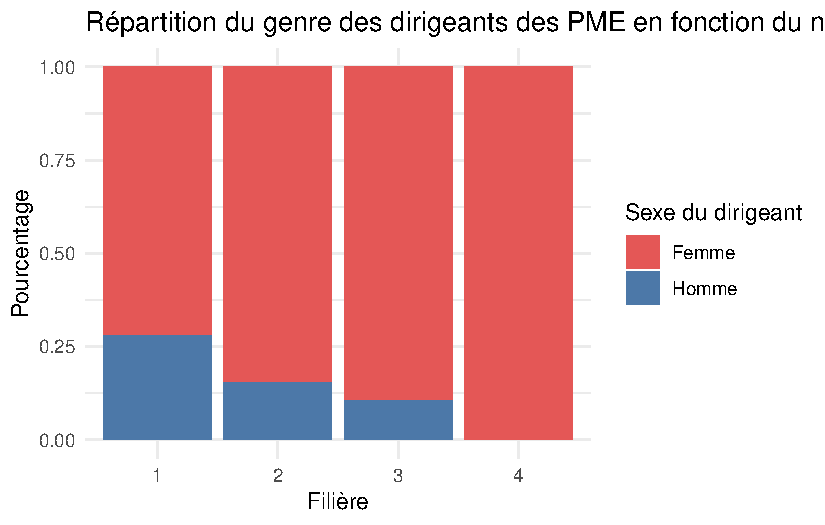
\includegraphics{projet_R_files/figure-pdf/unnamed-chunk-31-1.pdf}

}

\end{figure}

\begin{itemize}
\tightlist
\item
  Répartition du sexe du dirigeant/responsable de la PME par filière
  unique
\end{itemize}

\begin{Shaded}
\begin{Highlighting}[]
\DocumentationTok{\#\#\#\#************ pour une filiere *****************}\AlertTok{\#\#\#}
\CommentTok{\# Subset des données pour les variables d\textquotesingle{}intérêt}
\NormalTok{data\_subset }\OtherTok{\textless{}{-}}\NormalTok{ projet }\SpecialCharTok{\%\textgreater{}\%} \FunctionTok{filter}\NormalTok{(filiere}\SpecialCharTok{==}\DecValTok{1}\NormalTok{) }\SpecialCharTok{\%\textgreater{}\%} \FunctionTok{select}\NormalTok{(sexe, nom\_filiere)}


\CommentTok{\# Répartition du sexe du dirigeant/responsable de la PME par filière}

\FunctionTok{ggplot}\NormalTok{(data\_subset, }\FunctionTok{aes}\NormalTok{(}\AttributeTok{x =}\NormalTok{ nom\_filiere, }\AttributeTok{fill =}\NormalTok{ sexe)) }\SpecialCharTok{+}
  \FunctionTok{geom\_bar}\NormalTok{(}\AttributeTok{position =} \StringTok{"fill"}\NormalTok{) }\SpecialCharTok{+}
  \FunctionTok{labs}\NormalTok{(}\AttributeTok{x =} \StringTok{"Filière\_unique"}\NormalTok{, }\AttributeTok{y =} \StringTok{"Pourcentage"}\NormalTok{, }\AttributeTok{fill =} \StringTok{"Sexe du dirigeant"}\NormalTok{) }\SpecialCharTok{+}
  \FunctionTok{scale\_fill\_manual}\NormalTok{(}\AttributeTok{values =} \FunctionTok{c}\NormalTok{(}\StringTok{"\#4C78A8"}\NormalTok{, }\StringTok{"\#E45756"}\NormalTok{), }\AttributeTok{labels =} \FunctionTok{c}\NormalTok{(}\StringTok{"Homme"}\NormalTok{, }\StringTok{"Femme"}\NormalTok{)) }\SpecialCharTok{+}
  \FunctionTok{theme\_minimal}\NormalTok{() }\SpecialCharTok{+}
  \FunctionTok{labs}\NormalTok{(}\AttributeTok{title =} \StringTok{"Répartition du genre des dirigeants des PME en fonction du nombre de filières"}\NormalTok{)}
\end{Highlighting}
\end{Shaded}

\begin{figure}[H]

{\centering 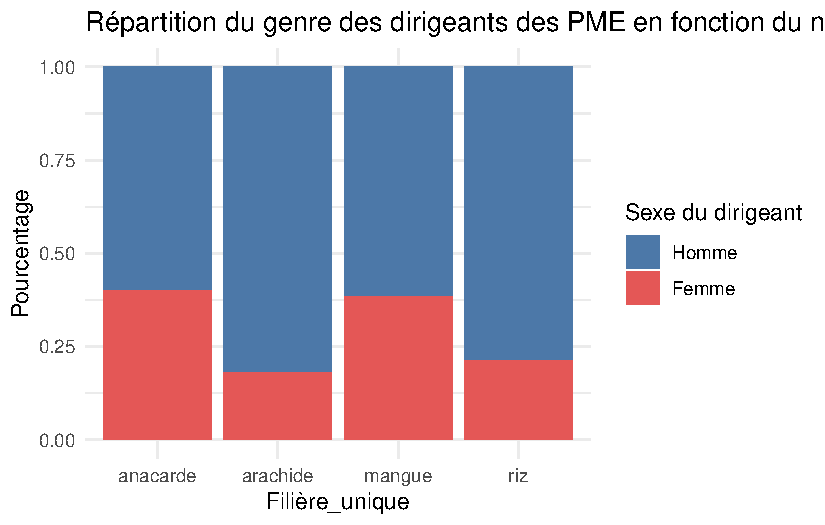
\includegraphics{projet_R_files/figure-pdf/unnamed-chunk-32-1.pdf}

}

\end{figure}

\begin{itemize}
\tightlist
\item
  Répartition du sexe du dirigeant/responsable de la PME pour deux
  filières
\end{itemize}

\begin{Shaded}
\begin{Highlighting}[]
\DocumentationTok{\#\#\#\#************ pour deux filiere *****************}\AlertTok{\#\#\#}
\CommentTok{\# Subset des données pour les variables d\textquotesingle{}intérêt}
\NormalTok{data\_subset }\OtherTok{\textless{}{-}}\NormalTok{ projet }\SpecialCharTok{\%\textgreater{}\%} \FunctionTok{filter}\NormalTok{(filiere}\SpecialCharTok{==}\DecValTok{2}\NormalTok{) }\SpecialCharTok{\%\textgreater{}\%} \FunctionTok{select}\NormalTok{(sexe, nom\_filiere)}


\CommentTok{\# Répartition du sexe du dirigeant/responsable de la PME par filière}
\FunctionTok{ggplot}\NormalTok{(data\_subset, }\FunctionTok{aes}\NormalTok{(}\AttributeTok{x =}\NormalTok{ nom\_filiere, }\AttributeTok{fill =}\NormalTok{ sexe)) }\SpecialCharTok{+}
  \FunctionTok{geom\_bar}\NormalTok{(}\AttributeTok{position =} \StringTok{"fill"}\NormalTok{) }\SpecialCharTok{+}
  \FunctionTok{labs}\NormalTok{(}\AttributeTok{x =} \StringTok{"groupe\_Filière(2)"}\NormalTok{, }\AttributeTok{y =} \StringTok{"Pourcentage"}\NormalTok{, }\AttributeTok{fill =} \StringTok{"Sexe du dirigeant"}\NormalTok{) }\SpecialCharTok{+}
  \FunctionTok{scale\_fill\_manual}\NormalTok{(}\AttributeTok{values =} \FunctionTok{c}\NormalTok{(}\StringTok{"\#4C78A8"}\NormalTok{, }\StringTok{"\#E45756"}\NormalTok{), }\AttributeTok{labels =} \FunctionTok{c}\NormalTok{(}\StringTok{"Homme"}\NormalTok{, }\StringTok{"Femme"}\NormalTok{)) }\SpecialCharTok{+}
  \FunctionTok{theme\_minimal}\NormalTok{()}\SpecialCharTok{+}
  \FunctionTok{labs}\NormalTok{(}\AttributeTok{title =} \StringTok{"Répartition du genre des dirigeants des PMEen fonction des filieres"}\NormalTok{)}
\end{Highlighting}
\end{Shaded}

\begin{figure}[H]

{\centering 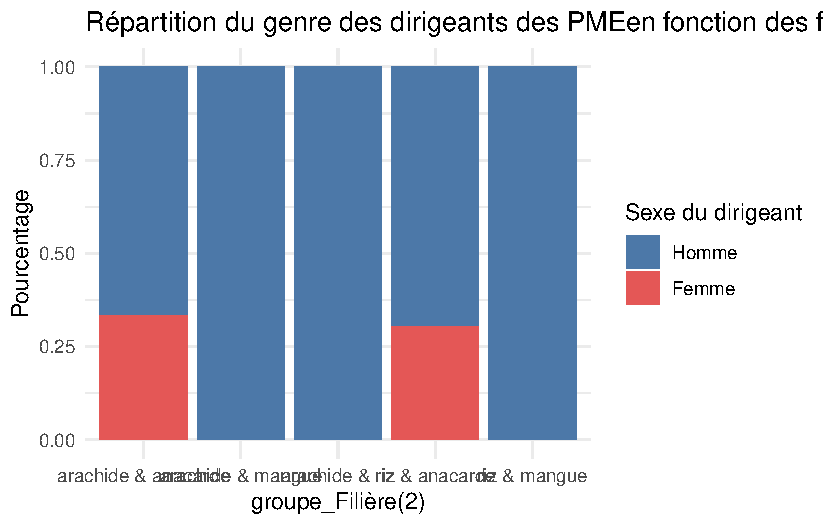
\includegraphics{projet_R_files/figure-pdf/unnamed-chunk-33-1.pdf}

}

\end{figure}

\begin{itemize}
\tightlist
\item
  Répartition du sexe du dirigeant/responsable de la PME pour plus de
  deux filières
\end{itemize}

\begin{Shaded}
\begin{Highlighting}[]
\DocumentationTok{\#\#\#\#************ pour plus de deux filiere *****************}\AlertTok{\#\#\#}
\CommentTok{\# Subset des données pour les variables d\textquotesingle{}intérêt}
\NormalTok{data\_subset }\OtherTok{\textless{}{-}}\NormalTok{ projet }\SpecialCharTok{\%\textgreater{}\%} \FunctionTok{filter}\NormalTok{(filiere}\SpecialCharTok{==}\DecValTok{3} \SpecialCharTok{|}\NormalTok{filiere}\SpecialCharTok{==}\DecValTok{4}\NormalTok{) }\SpecialCharTok{\%\textgreater{}\%} \FunctionTok{select}\NormalTok{(sexe, nom\_filiere)}
\CommentTok{\# Répartition du sexe du dirigeant/responsable de la PME par filière}
\FunctionTok{ggplot}\NormalTok{(data\_subset, }\FunctionTok{aes}\NormalTok{(}\AttributeTok{x =}\NormalTok{ nom\_filiere, }\AttributeTok{fill =}\NormalTok{ sexe)) }\SpecialCharTok{+}
  \FunctionTok{geom\_bar}\NormalTok{(}\AttributeTok{position =} \StringTok{"fill"}\NormalTok{) }\SpecialCharTok{+}
  \FunctionTok{labs}\NormalTok{(}\AttributeTok{x =} \StringTok{"groupe\_Filière(au moins3)"}\NormalTok{, }\AttributeTok{y =} \StringTok{"Pourcentage"}\NormalTok{, }\AttributeTok{fill =} \StringTok{"Sexe du dirigeant"}\NormalTok{) }\SpecialCharTok{+}
  \FunctionTok{scale\_fill\_manual}\NormalTok{(}\AttributeTok{values =} \FunctionTok{c}\NormalTok{(}\StringTok{"\#4C78A8"}\NormalTok{, }\StringTok{"\#E45756"}\NormalTok{), }\AttributeTok{labels =} \FunctionTok{c}\NormalTok{(}\StringTok{"Homme"}\NormalTok{, }\StringTok{"Femme"}\NormalTok{)) }\SpecialCharTok{+}
  \FunctionTok{theme\_minimal}\NormalTok{()}\SpecialCharTok{+} 
  \FunctionTok{labs}\NormalTok{(}\AttributeTok{title =} \StringTok{"Répartition du genre des dirigeants des PMEen fonction des filieres"}\NormalTok{)}
\end{Highlighting}
\end{Shaded}

\begin{figure}[H]

{\centering 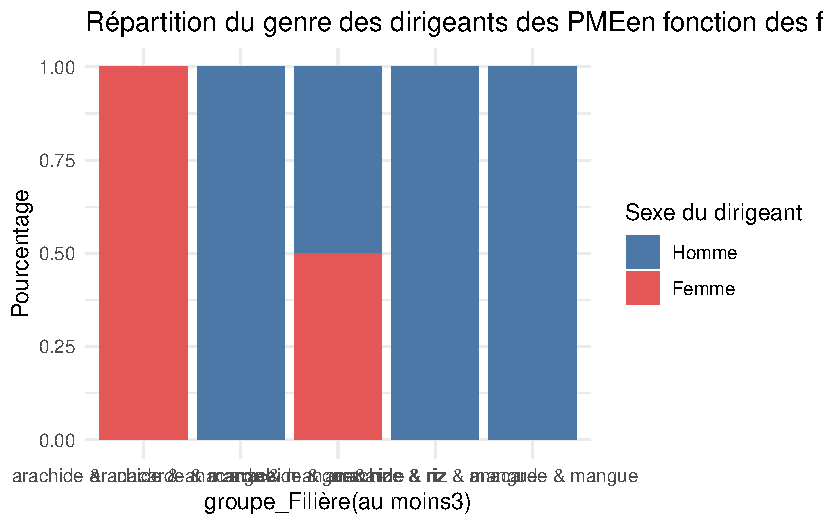
\includegraphics{projet_R_files/figure-pdf/unnamed-chunk-34-1.pdf}

}

\end{figure}

\begin{itemize}
\tightlist
\item
  Analyse de l'âge du dirigeant/responsable de la PME (variable q24)
  dans chaque filière pour déterminer les tendances générationnelles.
  Analysez Propriétaire/locataire dans chaque filière
\end{itemize}

\begin{Shaded}
\begin{Highlighting}[]
\CommentTok{\# Répartition du sexe du dirigeant/responsable de la PME par filière}
\FunctionTok{ggplot}\NormalTok{(projet, }\FunctionTok{aes}\NormalTok{(}\AttributeTok{x =}\NormalTok{ filiere, }\AttributeTok{fill =}\NormalTok{ q81)) }\SpecialCharTok{+}
  \FunctionTok{geom\_bar}\NormalTok{(}\AttributeTok{position =} \StringTok{"fill"}\NormalTok{) }\SpecialCharTok{+}
  \FunctionTok{labs}\NormalTok{(}\AttributeTok{x =} \StringTok{"Nombre de  Filière"}\NormalTok{, }\AttributeTok{y =} \StringTok{"Pourcentage"}\NormalTok{, }\AttributeTok{fill =} \StringTok{"Sexe du dirigeant"}\NormalTok{) }\SpecialCharTok{+}
  \FunctionTok{scale\_fill\_manual}\NormalTok{(}\AttributeTok{values =} \FunctionTok{c}\NormalTok{( }\StringTok{"\#E45756"}\NormalTok{,}\StringTok{"\#4C78A8"}\NormalTok{), }\AttributeTok{labels =} \FunctionTok{c}\NormalTok{(}\StringTok{"Locataire"}\NormalTok{,}\StringTok{"Propriétaire"}\NormalTok{)) }\SpecialCharTok{+}
  \FunctionTok{theme\_minimal}\NormalTok{()}\SpecialCharTok{+}
  \FunctionTok{labs}\NormalTok{(}\AttributeTok{title =} \StringTok{"Répartition du genre des dirigeants des PMEen fonction des filieres"}\NormalTok{)}
\end{Highlighting}
\end{Shaded}

\begin{figure}[H]

{\centering 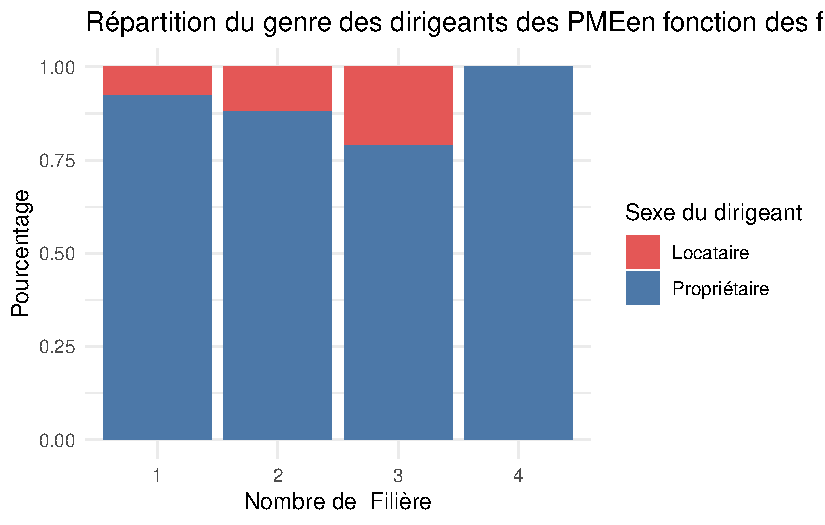
\includegraphics{projet_R_files/figure-pdf/unnamed-chunk-35-1.pdf}

}

\end{figure}

\hypertarget{un-peu-de-cartographie}{%
\subsection{3. Un peu de cartographie}\label{un-peu-de-cartographie}}

\hypertarget{transformation-le-data.frame-en-donnuxe9es-guxe9ographiques-dont-lobjet-sera-nommuxe9-projet_map.}{%
\paragraph{\texorpdfstring{\emph{3.1. Transformation le data.frame en
données géographiques dont l'objet sera nommé
projet\_map.}}{3.1. Transformation le data.frame en données géographiques dont l'objet sera nommé projet\_map.}}\label{transformation-le-data.frame-en-donnuxe9es-guxe9ographiques-dont-lobjet-sera-nommuxe9-projet_map.}}

\begin{Shaded}
\begin{Highlighting}[]
\CommentTok{\# Création de l\textquotesingle{}objet projet\_map avec des données géographiques}
\NormalTok{projet\_map }\OtherTok{\textless{}{-}}\NormalTok{ projet }\SpecialCharTok{\%\textgreater{}\%}
  \FunctionTok{st\_as\_sf}\NormalTok{(}\AttributeTok{coords =} \FunctionTok{c}\NormalTok{(}\StringTok{"gps\_menlongitude"}\NormalTok{, }\StringTok{"gps\_menlatitude"}\NormalTok{), }\AttributeTok{crs =} \DecValTok{4326}\NormalTok{)}

\CommentTok{\#Ceci provient du referentiel mondiale}
\end{Highlighting}
\end{Shaded}

\hypertarget{ruxe9pruxe9sentation-spatiale-des-pme-suivant-le-sexe}{%
\paragraph{\texorpdfstring{\emph{3.2. Réprésentation spatiale des PME
suivant le
sexe}}{3.2. Réprésentation spatiale des PME suivant le sexe}}\label{ruxe9pruxe9sentation-spatiale-des-pme-suivant-le-sexe}}

\begin{itemize}
\tightlist
\item
  Création de la carte spatiale des PME selon le sexe
\end{itemize}

\begin{Shaded}
\begin{Highlighting}[]
\CommentTok{\# Création de la carte spatiale des PME selon le sexe}
\FunctionTok{ggplot}\NormalTok{() }\SpecialCharTok{+}
  \FunctionTok{geom\_sf}\NormalTok{(}\AttributeTok{data =}\NormalTok{ projet\_map, }\FunctionTok{aes}\NormalTok{(}\AttributeTok{color =}\NormalTok{ sexe)) }\SpecialCharTok{+}
  \FunctionTok{scale\_color\_manual}\NormalTok{(}\AttributeTok{values =} \FunctionTok{c}\NormalTok{( }\StringTok{"pink"}\NormalTok{,}\StringTok{"darkgreen"}\NormalTok{)) }\SpecialCharTok{+}  \CommentTok{\# Couleurs des catégories de sexe (à personnaliser)}
  \FunctionTok{labs}\NormalTok{(}\AttributeTok{color =} \StringTok{"Sexe"}\NormalTok{) }\SpecialCharTok{+}
  \FunctionTok{theme\_minimal}\NormalTok{()}\SpecialCharTok{+}
  \FunctionTok{labs}\NormalTok{(}\AttributeTok{title =} \StringTok{"Répartition des PME selon le sexe du dirigeant"}\NormalTok{)}
\end{Highlighting}
\end{Shaded}

\begin{figure}[H]

{\centering 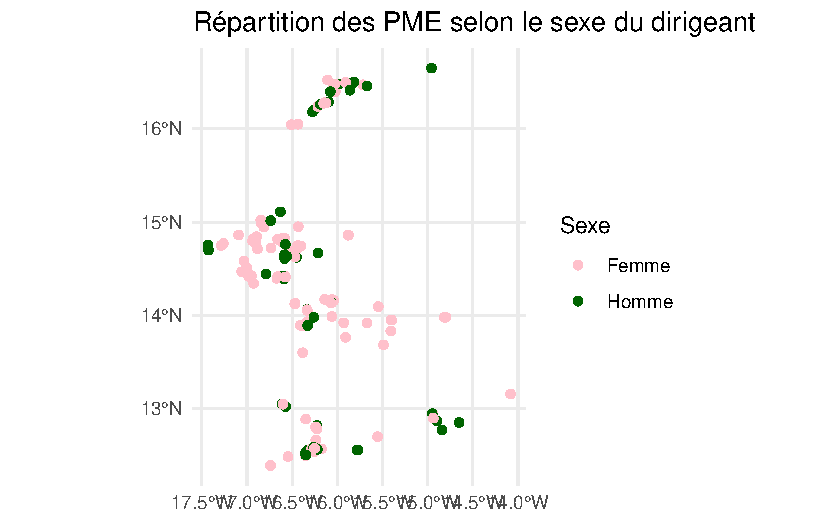
\includegraphics{projet_R_files/figure-pdf/unnamed-chunk-37-1.pdf}

}

\end{figure}

\begin{itemize}
\tightlist
\item
  Pour une meilleure presentation ajoutons la carte du senegal
\end{itemize}

\textbf{Chargement des coordonnées géographiques de la région du pays}

\begin{verbatim}
Multiple layers are present in data source C:\Users\HP\Desktop\moi 22-23\sm2\R\Durel_Valdes_NZIALI_TCHAMOU\data\sen.gpkg, reading layer `sen_adm3'.
Use `st_layers' to list all layer names and their type in a data source.
Set the `layer' argument in `st_read' to read a particular layer.
Reading layer `sen_adm3' from data source 
  `C:\Users\HP\Desktop\moi 22-23\sm2\R\Durel_Valdes_NZIALI_TCHAMOU\data\sen.gpkg' 
  using driver `GPKG'
Simple feature collection with 121 features and 8 fields
Geometry type: MULTIPOLYGON
Dimension:     XY
Bounding box:  xmin: -17.53092 ymin: 12.30777 xmax: -11.34801 ymax: 16.69373
Geodetic CRS:  WGS 84
\end{verbatim}

\textbf{Création de la carte spatiale des PME selon le sexe et la région
avec la région en arrière-plan}

\begin{Shaded}
\begin{Highlighting}[]
\CommentTok{\# Création de la carte spatiale des PME selon le sexe et la région avec la région en arrière{-}plan}
\FunctionTok{ggplot}\NormalTok{() }\SpecialCharTok{+}
  \FunctionTok{geom\_sf}\NormalTok{(}\AttributeTok{data =}\NormalTok{ OCCreg, }\AttributeTok{color =} \StringTok{"lightgray"}\NormalTok{) }\SpecialCharTok{+}  \CommentTok{\# Carte de la région en arrière{-}plan}
  \FunctionTok{geom\_sf\_label}\NormalTok{(}\AttributeTok{data =}\NormalTok{ OCCreg, }\FunctionTok{aes}\NormalTok{(}\AttributeTok{label =}\NormalTok{ adm1\_name), }\AttributeTok{color =} \StringTok{"black"}\NormalTok{, }\AttributeTok{size =} \DecValTok{2}\NormalTok{)}\SpecialCharTok{+}
  \FunctionTok{coord\_sf}\NormalTok{() }\SpecialCharTok{+}
  \FunctionTok{geom\_sf}\NormalTok{(}\AttributeTok{data =}\NormalTok{ projet\_map, }\FunctionTok{aes}\NormalTok{(}\AttributeTok{color =}\NormalTok{ sexe)) }\SpecialCharTok{+}
  \FunctionTok{scale\_color\_manual}\NormalTok{(}\AttributeTok{values =} \FunctionTok{c}\NormalTok{(}\StringTok{"blue"}\NormalTok{, }\StringTok{"pink"}\NormalTok{)) }\SpecialCharTok{+}  \CommentTok{\# Couleurs des catégories de sexe (à personnaliser)}
  \FunctionTok{labs}\NormalTok{(}\AttributeTok{color =} \StringTok{"Genre"}\NormalTok{) }\SpecialCharTok{+}
  \FunctionTok{theme\_minimal}\NormalTok{()}\SpecialCharTok{+}\FunctionTok{theme}\NormalTok{(}\AttributeTok{panel.background =} \FunctionTok{element\_rect}\NormalTok{(}\AttributeTok{fill =} \StringTok{"azure"}\NormalTok{,}\AttributeTok{color=}\ConstantTok{NA}\NormalTok{)) }\SpecialCharTok{+}
  \FunctionTok{annotation\_north\_arrow}\NormalTok{(}\AttributeTok{location =} \StringTok{"tl"}\NormalTok{, }\AttributeTok{which\_north =} \StringTok{"true"}\NormalTok{, }\AttributeTok{style =}\NormalTok{ north\_arrow\_orienteering)}\SpecialCharTok{+}
  \FunctionTok{annotation\_scale}\NormalTok{(}\AttributeTok{location =} \StringTok{"bl"}\NormalTok{, }\AttributeTok{width\_hint =} \FloatTok{0.2}\NormalTok{)}\SpecialCharTok{+}
  \FunctionTok{labs}\NormalTok{(}\AttributeTok{title =} \StringTok{"Répartition géographique des PME selon le genre du dirigeant"}\NormalTok{)}
\end{Highlighting}
\end{Shaded}

\begin{figure}[H]

{\centering 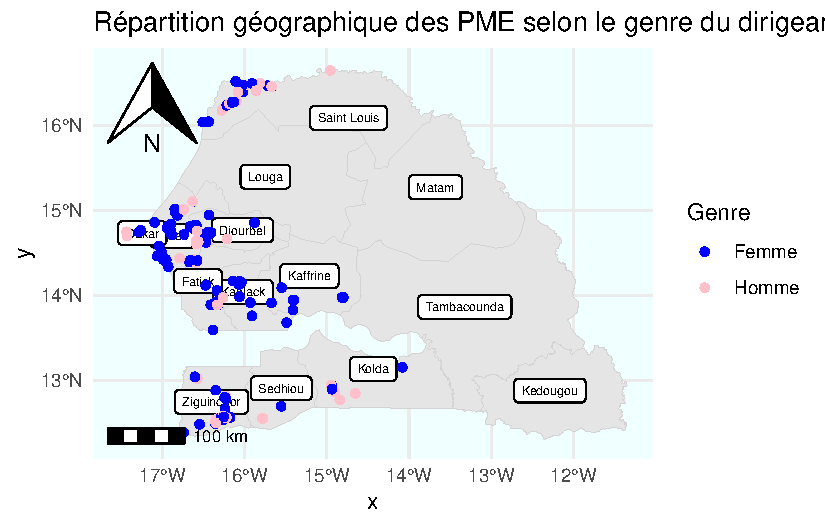
\includegraphics{projet_R_files/figure-pdf/unnamed-chunk-39-1.pdf}

}

\end{figure}

\hypertarget{faites-une-ruxe9pruxe9sentation-spatiale-des-pme-suivant-le-niveau-dinstruction}{%
\paragraph{\texorpdfstring{\emph{3.3. Faites une réprésentation spatiale
des PME suivant le niveau
d'instruction}}{3.3. Faites une réprésentation spatiale des PME suivant le niveau d'instruction}}\label{faites-une-ruxe9pruxe9sentation-spatiale-des-pme-suivant-le-niveau-dinstruction}}

\begin{Shaded}
\begin{Highlighting}[]
\CommentTok{\# Création de la carte spatiale des PME selon le sexe}
\FunctionTok{ggplot}\NormalTok{() }\SpecialCharTok{+}
  \FunctionTok{geom\_sf}\NormalTok{(}\AttributeTok{data =}\NormalTok{ OCCreg, }\AttributeTok{color =} \StringTok{"lightgray"}\NormalTok{) }\SpecialCharTok{+}  \CommentTok{\# Carte de la région en arrière{-}plan}
  \FunctionTok{geom\_sf\_label}\NormalTok{(}\AttributeTok{data =}\NormalTok{ OCCreg, }\FunctionTok{aes}\NormalTok{(}\AttributeTok{label =}\NormalTok{ adm1\_name), }\AttributeTok{color =} \StringTok{"black"}\NormalTok{, }\AttributeTok{size =} \DecValTok{2}\NormalTok{)}\SpecialCharTok{+}
  \FunctionTok{coord\_sf}\NormalTok{() }\SpecialCharTok{+}
  \FunctionTok{geom\_sf}\NormalTok{(}\AttributeTok{data =}\NormalTok{ projet\_map, }\FunctionTok{aes}\NormalTok{(}\AttributeTok{color =}\NormalTok{ q25)) }\SpecialCharTok{+}
  \FunctionTok{scale\_fill\_manual}\NormalTok{(}\AttributeTok{values =} \FunctionTok{c}\NormalTok{(}\StringTok{"\#E45756"}\NormalTok{, }\StringTok{"\#4C78A8"}\NormalTok{,}\StringTok{"darkgreen"}\NormalTok{,}\StringTok{"blue"}\NormalTok{)) }\SpecialCharTok{+}  \CommentTok{\# Couleurs des catégories de sexe (à personnaliser)}
  \FunctionTok{labs}\NormalTok{(}\AttributeTok{color =} \StringTok{"niveau d\textquotesingle{}instruction"}\NormalTok{) }\SpecialCharTok{+}
  \FunctionTok{theme\_minimal}\NormalTok{()}\SpecialCharTok{+}
  \FunctionTok{theme}\NormalTok{(}\AttributeTok{panel.background =} \FunctionTok{element\_rect}\NormalTok{(}\AttributeTok{fill =} \StringTok{"azure"}\NormalTok{,}\AttributeTok{color=}\ConstantTok{NA}\NormalTok{)) }\SpecialCharTok{+}
  \FunctionTok{annotation\_north\_arrow}\NormalTok{(}\AttributeTok{location =} \StringTok{"tl"}\NormalTok{, }\AttributeTok{which\_north =} \StringTok{"true"}\NormalTok{, }\AttributeTok{style =}\NormalTok{ north\_arrow\_orienteering)}\SpecialCharTok{+}
  \FunctionTok{annotation\_scale}\NormalTok{(}\AttributeTok{location =} \StringTok{"bl"}\NormalTok{, }\AttributeTok{width\_hint =} \FloatTok{0.2}\NormalTok{)}\SpecialCharTok{+}
  \FunctionTok{labs}\NormalTok{(}\AttributeTok{title =} \StringTok{"Répartition géographique des PME selon le niveau d\textquotesingle{}instruction du dirigeant"}\NormalTok{)}
\end{Highlighting}
\end{Shaded}

\begin{figure}[H]

{\centering 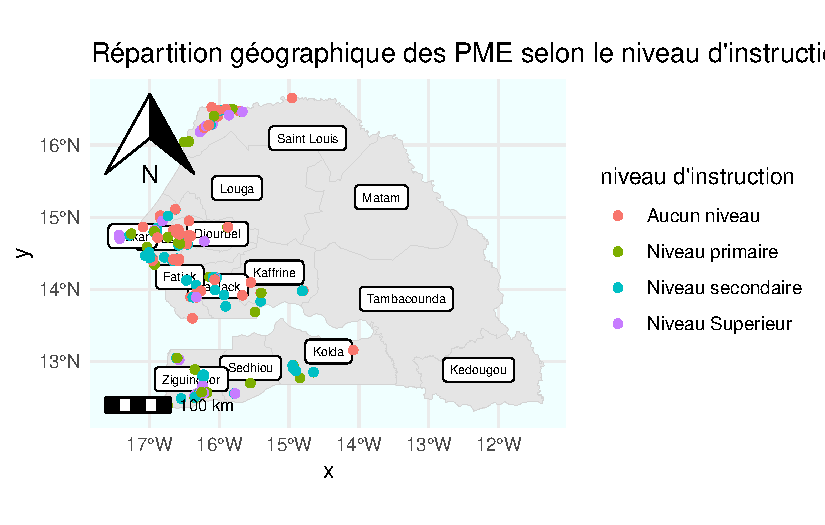
\includegraphics{projet_R_files/figure-pdf/unnamed-chunk-40-1.pdf}

}

\end{figure}

\hypertarget{analyse-spatiale-de-choix}{%
\paragraph{\texorpdfstring{\textbf{3.4. Analyse spatiale de
choix}}{3.4. Analyse spatiale de choix}}\label{analyse-spatiale-de-choix}}

\hypertarget{ruxe9partition-guxe9ographiquedes-pme-selon-le-nombre-de-filiuxe8res}{%
\subparagraph{3.4.1. Répartition géographiquedes PME selon le nombre de
filières}\label{ruxe9partition-guxe9ographiquedes-pme-selon-le-nombre-de-filiuxe8res}}

\begin{Shaded}
\begin{Highlighting}[]
\CommentTok{\# répartition géographiquedes PME selon les filiere}
\FunctionTok{ggplot}\NormalTok{() }\SpecialCharTok{+}
  \FunctionTok{geom\_sf}\NormalTok{(}\AttributeTok{data =}\NormalTok{ OCCreg, }\AttributeTok{color =} \StringTok{"lightgray"}\NormalTok{) }\SpecialCharTok{+}  \CommentTok{\# Carte de la région en arrière{-}plan}
  \FunctionTok{geom\_sf\_label}\NormalTok{(}\AttributeTok{data =}\NormalTok{ OCCreg, }\FunctionTok{aes}\NormalTok{(}\AttributeTok{label =}\NormalTok{ adm1\_name), }\AttributeTok{color =} \StringTok{"black"}\NormalTok{, }\AttributeTok{size =} \DecValTok{2}\NormalTok{)}\SpecialCharTok{+}
  \FunctionTok{coord\_sf}\NormalTok{() }\SpecialCharTok{+}
  \FunctionTok{geom\_sf}\NormalTok{(}\AttributeTok{data =}\NormalTok{ projet\_map, }\FunctionTok{aes}\NormalTok{(}\AttributeTok{color =}\NormalTok{ nom\_filiere)) }\SpecialCharTok{+}
  \FunctionTok{scale\_fill\_manual}\NormalTok{(}\AttributeTok{values =} \FunctionTok{c}\NormalTok{(}\StringTok{"\#E45756"}\NormalTok{, }\StringTok{"\#4C78A8"}\NormalTok{,}\StringTok{"darkgreen"}\NormalTok{,}\StringTok{"blue"}\NormalTok{)) }\SpecialCharTok{+}  \CommentTok{\# Couleurs des catégories de sexe (à personnaliser)}
  \FunctionTok{labs}\NormalTok{(}\AttributeTok{color =} \StringTok{"filiere"}\NormalTok{) }\SpecialCharTok{+}
  \FunctionTok{theme\_minimal}\NormalTok{()}\SpecialCharTok{+}
  \FunctionTok{theme}\NormalTok{(}\AttributeTok{panel.background =} \FunctionTok{element\_rect}\NormalTok{(}\AttributeTok{fill =} \StringTok{"azure"}\NormalTok{,}\AttributeTok{color=}\ConstantTok{NA}\NormalTok{)) }\SpecialCharTok{+}
  \FunctionTok{annotation\_north\_arrow}\NormalTok{(}\AttributeTok{location =} \StringTok{"tl"}\NormalTok{, }\AttributeTok{which\_north =} \StringTok{"true"}\NormalTok{, }\AttributeTok{style =}\NormalTok{ north\_arrow\_orienteering)}\SpecialCharTok{+}
  \FunctionTok{annotation\_scale}\NormalTok{(}\AttributeTok{location =} \StringTok{"bl"}\NormalTok{, }\AttributeTok{width\_hint =} \FloatTok{0.2}\NormalTok{)}\SpecialCharTok{+}
  \FunctionTok{labs}\NormalTok{(}\AttributeTok{title =} \StringTok{"Répartition géographique des PME selon les filières"}\NormalTok{)}
\end{Highlighting}
\end{Shaded}

\begin{figure}[H]

{\centering 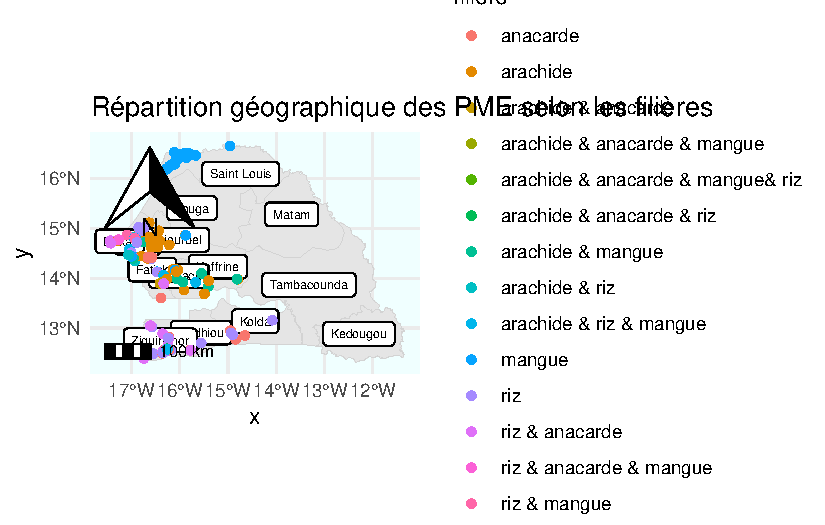
\includegraphics{projet_R_files/figure-pdf/unnamed-chunk-41-1.pdf}

}

\end{figure}

\begin{itemize}
\tightlist
\item
  Répartition géographiquedes PME qui font dans une seule culture
\end{itemize}

\begin{Shaded}
\begin{Highlighting}[]
\CommentTok{\# répartition géographiquedes PME qui font dans une seule culture}
\NormalTok{projet\_map1}\OtherTok{\textless{}{-}}\NormalTok{projet\_map }\SpecialCharTok{\%\textgreater{}\%} \FunctionTok{filter}\NormalTok{(filiere}\SpecialCharTok{==}\DecValTok{1}\NormalTok{) }\CommentTok{\# filtre les PME qui font dans une seule filiere}
\FunctionTok{ggplot}\NormalTok{() }\SpecialCharTok{+}
  \FunctionTok{geom\_sf}\NormalTok{(}\AttributeTok{data =}\NormalTok{ OCCreg, }\AttributeTok{color =} \StringTok{"lightgray"}\NormalTok{) }\SpecialCharTok{+}  \CommentTok{\# Carte de la région en arrière{-}plan}
  \FunctionTok{geom\_sf\_label}\NormalTok{(}\AttributeTok{data =}\NormalTok{ OCCreg, }\FunctionTok{aes}\NormalTok{(}\AttributeTok{label =}\NormalTok{ adm1\_name), }\AttributeTok{color =} \StringTok{"black"}\NormalTok{, }\AttributeTok{size =} \DecValTok{2}\NormalTok{)}\SpecialCharTok{+}
  \FunctionTok{coord\_sf}\NormalTok{() }\SpecialCharTok{+}
  \FunctionTok{geom\_sf}\NormalTok{(}\AttributeTok{data =}\NormalTok{ projet\_map1, }\FunctionTok{aes}\NormalTok{(}\AttributeTok{color =}\NormalTok{ nom\_filiere)) }\SpecialCharTok{+}
  \FunctionTok{scale\_fill\_manual}\NormalTok{(}\AttributeTok{values =} \FunctionTok{c}\NormalTok{(}\StringTok{"\#E45756"}\NormalTok{, }\StringTok{"\#4C78A8"}\NormalTok{,}\StringTok{"darkgreen"}\NormalTok{,}\StringTok{"blue"}\NormalTok{)) }\SpecialCharTok{+}  \CommentTok{\# Couleurs des catégories de sexe (à personnaliser)}
  \FunctionTok{labs}\NormalTok{(}\AttributeTok{color =} \StringTok{"filiere"}\NormalTok{) }\SpecialCharTok{+}
  \FunctionTok{theme\_minimal}\NormalTok{()}\SpecialCharTok{+}
  \FunctionTok{theme}\NormalTok{(}\AttributeTok{panel.background =} \FunctionTok{element\_rect}\NormalTok{(}\AttributeTok{fill =} \StringTok{"azure"}\NormalTok{,}\AttributeTok{color=}\ConstantTok{NA}\NormalTok{)) }\SpecialCharTok{+}
  \FunctionTok{annotation\_north\_arrow}\NormalTok{(}\AttributeTok{location =} \StringTok{"tl"}\NormalTok{, }\AttributeTok{which\_north =} \StringTok{"true"}\NormalTok{, }\AttributeTok{style =}\NormalTok{ north\_arrow\_orienteering)}\SpecialCharTok{+}
  \FunctionTok{annotation\_scale}\NormalTok{(}\AttributeTok{location =} \StringTok{"bl"}\NormalTok{, }\AttributeTok{width\_hint =} \FloatTok{0.2}\NormalTok{)}\SpecialCharTok{+}
  \FunctionTok{labs}\NormalTok{(}\AttributeTok{title =} \StringTok{"Répartition géographique des PME selon les filières"}\NormalTok{)}
\end{Highlighting}
\end{Shaded}

\begin{figure}[H]

{\centering 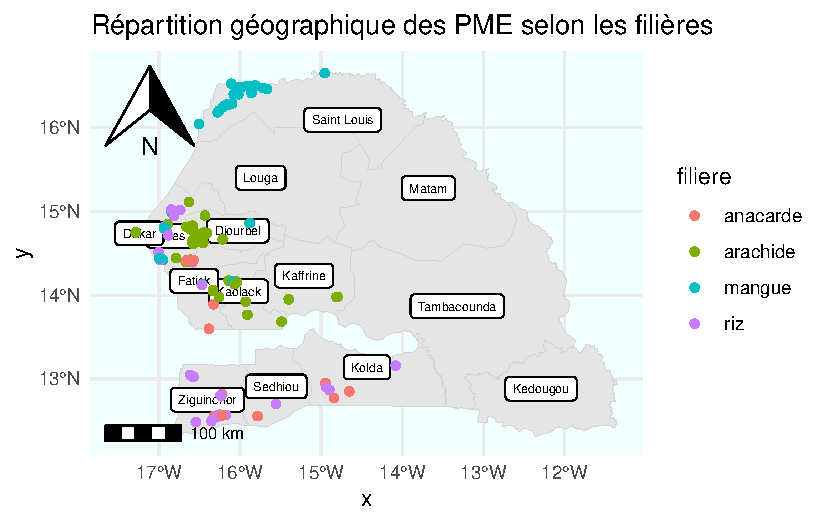
\includegraphics{projet_R_files/figure-pdf/unnamed-chunk-42-1.pdf}

}

\end{figure}

Commencons donc à filtrer notre carte\\

\begin{itemize}
\tightlist
\item
  Répartition géographique des PME qui font dans deux culture\\
\end{itemize}

\begin{Shaded}
\begin{Highlighting}[]
\CommentTok{\# répartition géographiquedes PME qui font dans deux  culture}
\NormalTok{projet\_map1}\OtherTok{\textless{}{-}}\NormalTok{projet\_map }\SpecialCharTok{\%\textgreater{}\%} \FunctionTok{filter}\NormalTok{(filiere}\SpecialCharTok{==}\DecValTok{2}\NormalTok{) }\CommentTok{\# filtre les PME qui font dans deux filiere}
\FunctionTok{ggplot}\NormalTok{() }\SpecialCharTok{+}
  \FunctionTok{geom\_sf}\NormalTok{(}\AttributeTok{data =}\NormalTok{ OCCreg, }\AttributeTok{color =} \StringTok{"lightgray"}\NormalTok{) }\SpecialCharTok{+}  \CommentTok{\# Carte de la région en arrière{-}plan}
  \FunctionTok{geom\_sf\_label}\NormalTok{(}\AttributeTok{data =}\NormalTok{ OCCreg, }\FunctionTok{aes}\NormalTok{(}\AttributeTok{label =}\NormalTok{ adm1\_name), }\AttributeTok{color =} \StringTok{"black"}\NormalTok{, }\AttributeTok{size =} \DecValTok{2}\NormalTok{)}\SpecialCharTok{+}
  \FunctionTok{coord\_sf}\NormalTok{() }\SpecialCharTok{+}
  \FunctionTok{geom\_sf}\NormalTok{(}\AttributeTok{data =}\NormalTok{ projet\_map1, }\FunctionTok{aes}\NormalTok{(}\AttributeTok{color =}\NormalTok{ nom\_filiere)) }\SpecialCharTok{+}
  \FunctionTok{scale\_fill\_manual}\NormalTok{(}\AttributeTok{values =} \FunctionTok{c}\NormalTok{(}\StringTok{"\#E45756"}\NormalTok{, }\StringTok{"\#4C78A8"}\NormalTok{,}\StringTok{"darkgreen"}\NormalTok{,}\StringTok{"blue"}\NormalTok{)) }\SpecialCharTok{+}  \CommentTok{\# Couleurs des catégories de sexe (à personnaliser)}
  \FunctionTok{labs}\NormalTok{(}\AttributeTok{color =} \StringTok{"filiere"}\NormalTok{) }\SpecialCharTok{+}
  \FunctionTok{theme\_minimal}\NormalTok{()}\SpecialCharTok{+}
  \FunctionTok{theme}\NormalTok{(}\AttributeTok{panel.background =} \FunctionTok{element\_rect}\NormalTok{(}\AttributeTok{fill =} \StringTok{"azure"}\NormalTok{,}\AttributeTok{color=}\ConstantTok{NA}\NormalTok{)) }\SpecialCharTok{+}
  \FunctionTok{annotation\_north\_arrow}\NormalTok{(}\AttributeTok{location =} \StringTok{"tl"}\NormalTok{, }\AttributeTok{which\_north =} \StringTok{"true"}\NormalTok{, }\AttributeTok{style =}\NormalTok{ north\_arrow\_orienteering)}\SpecialCharTok{+}
  \FunctionTok{annotation\_scale}\NormalTok{(}\AttributeTok{location =} \StringTok{"bl"}\NormalTok{, }\AttributeTok{width\_hint =} \FloatTok{0.2}\NormalTok{)}\SpecialCharTok{+}
  \FunctionTok{labs}\NormalTok{(}\AttributeTok{title =} \StringTok{"Répartition géographique des PME selon les filières"}\NormalTok{)}
\end{Highlighting}
\end{Shaded}

\begin{figure}[H]

{\centering 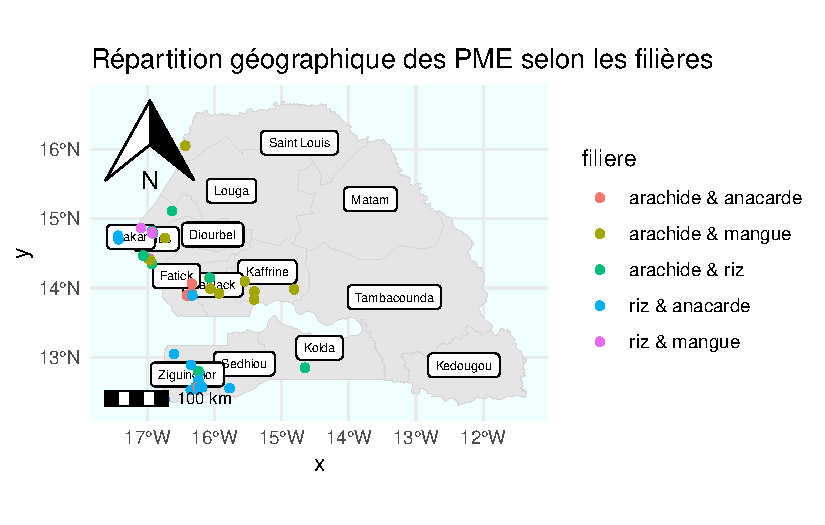
\includegraphics{projet_R_files/figure-pdf/unnamed-chunk-43-1.pdf}

}

\end{figure}

\begin{itemize}
\tightlist
\item
  Répartition géographique des PME qui font dans trois cultures
\end{itemize}

\begin{Shaded}
\begin{Highlighting}[]
\CommentTok{\# répartition géographiquedes PME qui font dans trois  culture}
\NormalTok{projet\_map1}\OtherTok{\textless{}{-}}\NormalTok{projet\_map }\SpecialCharTok{\%\textgreater{}\%} \FunctionTok{filter}\NormalTok{(filiere}\SpecialCharTok{==}\DecValTok{3}\NormalTok{) }\CommentTok{\# filtre les PME qui font dans trois filiere}
\FunctionTok{ggplot}\NormalTok{() }\SpecialCharTok{+}
  \FunctionTok{geom\_sf}\NormalTok{(}\AttributeTok{data =}\NormalTok{ OCCreg, }\AttributeTok{color =} \StringTok{"lightgray"}\NormalTok{) }\SpecialCharTok{+}  \CommentTok{\# Carte de la région en arrière{-}plan}
  \FunctionTok{geom\_sf\_label}\NormalTok{(}\AttributeTok{data =}\NormalTok{ OCCreg, }\FunctionTok{aes}\NormalTok{(}\AttributeTok{label =}\NormalTok{ adm1\_name), }\AttributeTok{color =} \StringTok{"black"}\NormalTok{, }\AttributeTok{size =} \DecValTok{2}\NormalTok{)}\SpecialCharTok{+}
  \FunctionTok{coord\_sf}\NormalTok{() }\SpecialCharTok{+}
  \FunctionTok{geom\_sf}\NormalTok{(}\AttributeTok{data =}\NormalTok{ projet\_map1, }\FunctionTok{aes}\NormalTok{(}\AttributeTok{color =}\NormalTok{ nom\_filiere)) }\SpecialCharTok{+}
  \FunctionTok{scale\_fill\_manual}\NormalTok{(}\AttributeTok{values =} \FunctionTok{c}\NormalTok{(}\StringTok{"\#E45756"}\NormalTok{, }\StringTok{"\#4C78A8"}\NormalTok{,}\StringTok{"darkgreen"}\NormalTok{,}\StringTok{"blue"}\NormalTok{)) }\SpecialCharTok{+}  \CommentTok{\# Couleurs des catégories de sexe (à personnaliser)}
  \FunctionTok{labs}\NormalTok{(}\AttributeTok{color =} \StringTok{"filiere"}\NormalTok{) }\SpecialCharTok{+}
  \FunctionTok{theme\_minimal}\NormalTok{()}\SpecialCharTok{+}
  \FunctionTok{theme}\NormalTok{(}\AttributeTok{panel.background =} \FunctionTok{element\_rect}\NormalTok{(}\AttributeTok{fill =} \StringTok{"azure"}\NormalTok{,}\AttributeTok{color=}\ConstantTok{NA}\NormalTok{)) }\SpecialCharTok{+}
  \FunctionTok{annotation\_north\_arrow}\NormalTok{(}\AttributeTok{location =} \StringTok{"tl"}\NormalTok{, }\AttributeTok{which\_north =} \StringTok{"true"}\NormalTok{, }\AttributeTok{style =}\NormalTok{ north\_arrow\_orienteering)}\SpecialCharTok{+}
  \FunctionTok{annotation\_scale}\NormalTok{(}\AttributeTok{location =} \StringTok{"bl"}\NormalTok{, }\AttributeTok{width\_hint =} \FloatTok{0.2}\NormalTok{)}\SpecialCharTok{+}
  \FunctionTok{labs}\NormalTok{(}\AttributeTok{title =} \StringTok{"Répartition géographique des PME selon les filières"}\NormalTok{)}
\end{Highlighting}
\end{Shaded}

\begin{figure}[H]

{\centering 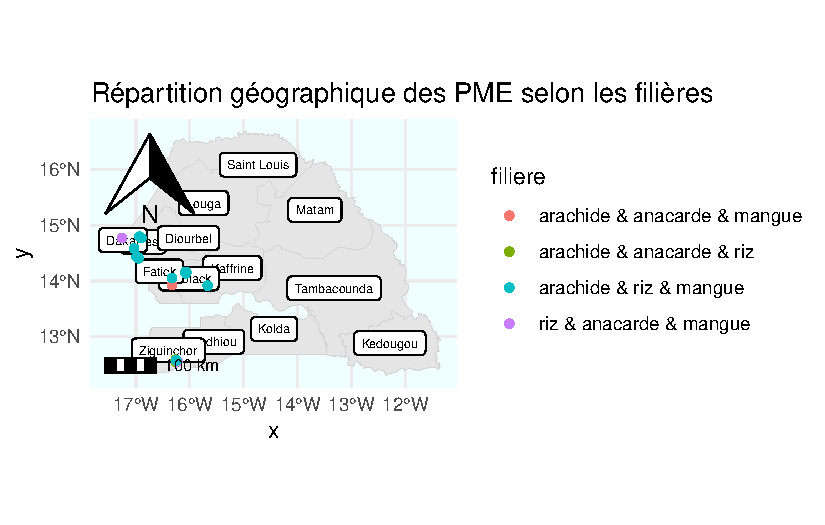
\includegraphics{projet_R_files/figure-pdf/unnamed-chunk-44-1.pdf}

}

\end{figure}

\begin{itemize}
\tightlist
\item
  Répartition géographiquedes PME qui font dans quatre cultures
\end{itemize}

\begin{Shaded}
\begin{Highlighting}[]
\CommentTok{\# répartition géographiquedes PME qui font dans quatre  culture}
\NormalTok{projet\_map1}\OtherTok{\textless{}{-}}\NormalTok{projet\_map }\SpecialCharTok{\%\textgreater{}\%} \FunctionTok{filter}\NormalTok{(filiere}\SpecialCharTok{==}\DecValTok{4}\NormalTok{) }\CommentTok{\# filtre les PME qui font dans quatre filiere}
\FunctionTok{ggplot}\NormalTok{() }\SpecialCharTok{+}
  \FunctionTok{geom\_sf}\NormalTok{(}\AttributeTok{data =}\NormalTok{ OCCreg, }\AttributeTok{color =} \StringTok{"lightgray"}\NormalTok{) }\SpecialCharTok{+}  \CommentTok{\# Carte de la région en arrière{-}plan}
  \FunctionTok{geom\_sf\_label}\NormalTok{(}\AttributeTok{data =}\NormalTok{ OCCreg, }\FunctionTok{aes}\NormalTok{(}\AttributeTok{label =}\NormalTok{ adm1\_name), }\AttributeTok{color =} \StringTok{"black"}\NormalTok{, }\AttributeTok{size =} \DecValTok{2}\NormalTok{)}\SpecialCharTok{+}
  \FunctionTok{coord\_sf}\NormalTok{() }\SpecialCharTok{+}
  \FunctionTok{geom\_sf}\NormalTok{(}\AttributeTok{data =}\NormalTok{ projet\_map1, }\FunctionTok{aes}\NormalTok{(}\AttributeTok{color =}\NormalTok{ nom\_filiere)) }\SpecialCharTok{+}
  \FunctionTok{scale\_fill\_manual}\NormalTok{(}\AttributeTok{values =} \FunctionTok{c}\NormalTok{(}\StringTok{"\#E45756"}\NormalTok{, }\StringTok{"\#4C78A8"}\NormalTok{,}\StringTok{"darkgreen"}\NormalTok{,}\StringTok{"blue"}\NormalTok{)) }\SpecialCharTok{+}  \CommentTok{\# Couleurs des catégories de sexe (à personnaliser)}
  \FunctionTok{labs}\NormalTok{(}\AttributeTok{color =} \StringTok{"filiere"}\NormalTok{) }\SpecialCharTok{+}
  \FunctionTok{theme\_minimal}\NormalTok{()}\SpecialCharTok{+}
  \FunctionTok{theme}\NormalTok{(}\AttributeTok{panel.background =} \FunctionTok{element\_rect}\NormalTok{(}\AttributeTok{fill =} \StringTok{"azure"}\NormalTok{,}\AttributeTok{color=}\ConstantTok{NA}\NormalTok{)) }\SpecialCharTok{+}
  \FunctionTok{annotation\_north\_arrow}\NormalTok{(}\AttributeTok{location =} \StringTok{"tl"}\NormalTok{, }\AttributeTok{which\_north =} \StringTok{"true"}\NormalTok{, }\AttributeTok{style =}\NormalTok{ north\_arrow\_orienteering)}\SpecialCharTok{+}
  \FunctionTok{annotation\_scale}\NormalTok{(}\AttributeTok{location =} \StringTok{"bl"}\NormalTok{, }\AttributeTok{width\_hint =} \FloatTok{0.2}\NormalTok{)}\SpecialCharTok{+}
  \FunctionTok{labs}\NormalTok{(}\AttributeTok{title =} \StringTok{"Répartition géographique des PME selon les filières"}\NormalTok{)}
\end{Highlighting}
\end{Shaded}

\begin{figure}[H]

{\centering 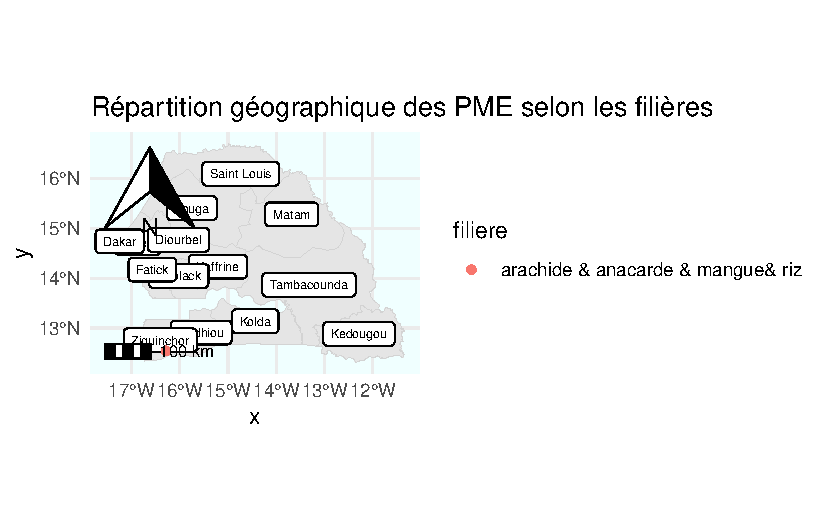
\includegraphics{projet_R_files/figure-pdf/unnamed-chunk-45-1.pdf}

}

\end{figure}

\hypertarget{uxe9valuez-si-les-pme-de-chaque-filiuxe8re-sont-desservies-par-des-routes-bitumuxe9es-et-examinez-luxe9tat-de-ces-routes.}{%
\subparagraph{3.4.2. Évaluez si les PME de chaque filière sont
desservies par des routes bitumées et examinez l'état de ces
routes.}\label{uxe9valuez-si-les-pme-de-chaque-filiuxe8re-sont-desservies-par-des-routes-bitumuxe9es-et-examinez-luxe9tat-de-ces-routes.}}

\begin{itemize}
\tightlist
\item
  Répartition géographiquedes PME selon les filiere desservies par des
  routes bitumées
\end{itemize}

\begin{Shaded}
\begin{Highlighting}[]
\CommentTok{\# répartition géographiquedes PME selon les filiere desservies par des routes bitumées (variable q16)}
\NormalTok{projet\_map1}\OtherTok{\textless{}{-}}\NormalTok{projet\_map }\SpecialCharTok{\%\textgreater{}\%} \FunctionTok{filter}\NormalTok{(filiere}\SpecialCharTok{==}\DecValTok{1}\NormalTok{) }\CommentTok{\# filtre les PME qui font dans une seule filiere}


\CommentTok{\# Création de la carte avec routes bitumées}

\FunctionTok{ggplot}\NormalTok{() }\SpecialCharTok{+}
  \FunctionTok{geom\_sf}\NormalTok{(}\AttributeTok{data =}\NormalTok{ OCCreg, }\AttributeTok{color =} \StringTok{"lightgray"}\NormalTok{) }\SpecialCharTok{+}
  \FunctionTok{geom\_sf\_label}\NormalTok{(}\AttributeTok{data =}\NormalTok{ OCCreg, }\FunctionTok{aes}\NormalTok{(}\AttributeTok{label =}\NormalTok{ adm1\_name), }\AttributeTok{color =} \StringTok{"black"}\NormalTok{, }\AttributeTok{size =} \DecValTok{2}\NormalTok{) }\SpecialCharTok{+}
  \FunctionTok{geom\_sf}\NormalTok{(}\AttributeTok{data =}\NormalTok{ projet\_map1, }\FunctionTok{aes}\NormalTok{(}\AttributeTok{fill =}\NormalTok{ nom\_filiere,}\AttributeTok{shape=}\NormalTok{ nom\_filiere, }\AttributeTok{color =}\NormalTok{ q16), }\AttributeTok{size =} \DecValTok{4}\NormalTok{ )}\SpecialCharTok{+}
  \FunctionTok{labs}\NormalTok{(}\AttributeTok{title =} \StringTok{"Répartition géographique des PME selon les filières et les routes"}\NormalTok{,}
       \AttributeTok{color =} \StringTok{"Approximitée d\textquotesingle{}une Route bitumée"}\NormalTok{) }\SpecialCharTok{+}
  \FunctionTok{theme\_minimal}\NormalTok{() }
\end{Highlighting}
\end{Shaded}

\begin{figure}[H]

{\centering 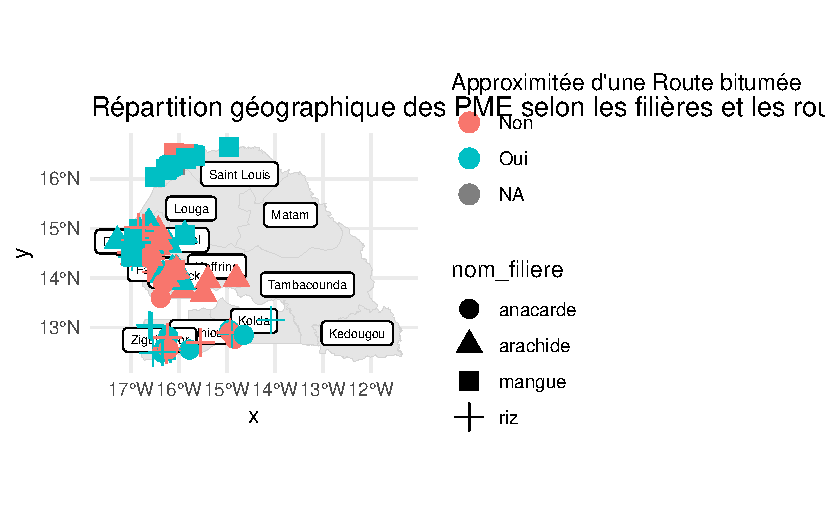
\includegraphics{projet_R_files/figure-pdf/unnamed-chunk-46-1.pdf}

}

\end{figure}

\begin{itemize}
\tightlist
\item
  Création de la carte avec l'état des routes bitumées
\end{itemize}

\begin{Shaded}
\begin{Highlighting}[]
\CommentTok{\# Création de la carte avec l\textquotesingle{}état des routes bitumées}

\NormalTok{projet\_map1}\OtherTok{\textless{}{-}}\NormalTok{projet\_map1 }\SpecialCharTok{\%\textgreater{}\%} \FunctionTok{filter}\NormalTok{(q16}\SpecialCharTok{==}\StringTok{"Oui"}\NormalTok{)}
\FunctionTok{ggplot}\NormalTok{() }\SpecialCharTok{+}
  \FunctionTok{geom\_sf}\NormalTok{(}\AttributeTok{data =}\NormalTok{ OCCreg, }\AttributeTok{color =} \StringTok{"lightgray"}\NormalTok{) }\SpecialCharTok{+}
  \FunctionTok{geom\_sf\_label}\NormalTok{(}\AttributeTok{data =}\NormalTok{ OCCreg, }\FunctionTok{aes}\NormalTok{(}\AttributeTok{label =}\NormalTok{ adm1\_name), }\AttributeTok{color =} \StringTok{"black"}\NormalTok{, }\AttributeTok{size =} \DecValTok{2}\NormalTok{) }\SpecialCharTok{+}
  \FunctionTok{geom\_sf}\NormalTok{(}\AttributeTok{data =}\NormalTok{ projet\_map1, }\FunctionTok{aes}\NormalTok{(}\AttributeTok{fill =}\NormalTok{ nom\_filiere,}\AttributeTok{shape=}\NormalTok{ nom\_filiere, }\AttributeTok{color =}\NormalTok{ q17) , }\AttributeTok{size=}\DecValTok{4}\NormalTok{)}\SpecialCharTok{+}
  \FunctionTok{labs}\NormalTok{(}\AttributeTok{title =} \StringTok{"Répartition géographique des PME selon les filières et les routes"}\NormalTok{,}
       \AttributeTok{color =} \StringTok{"Approximitée d\textquotesingle{}une Route bitumée"}\NormalTok{) }\SpecialCharTok{+}
  \FunctionTok{theme\_minimal}\NormalTok{() }
\end{Highlighting}
\end{Shaded}

\begin{figure}[H]

{\centering 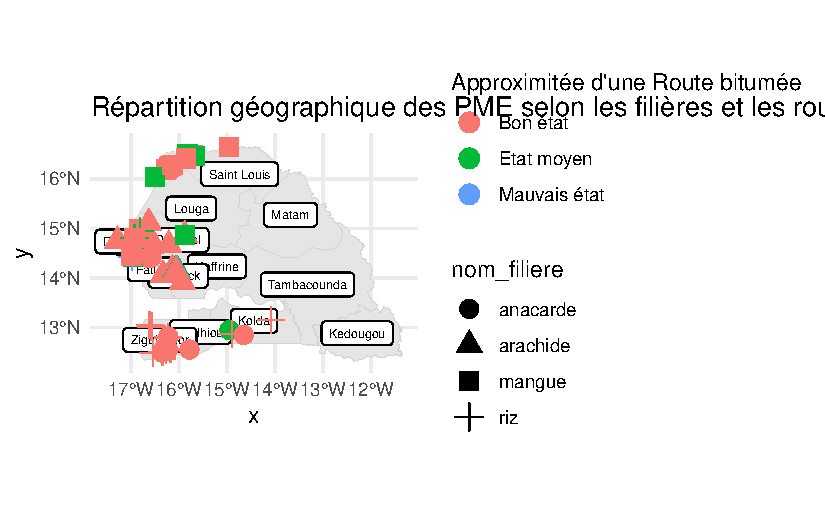
\includegraphics{projet_R_files/figure-pdf/unnamed-chunk-47-1.pdf}

}

\end{figure}

\hypertarget{partie-2}{%
\section{Partie 2}\label{partie-2}}

Le fichier excel Base\_Partie 2.xlsx contient un ensemble de données
artificielles créé dans le cadre de ce projet. La première feuille
contient des micro-données au niveau individuel des répondants à
l'enquête, la deuxième feuille contient des données pour les districts
dans lesquels les répondants de la première feuille ont été interrogés.
La troisième feuille contient des explications sur les variables
incluses dans toutes les feuilles précédentes.\\
\strut \\
\textbf{Chargement de données}

\begin{Shaded}
\begin{Highlighting}[]
\NormalTok{data }\OtherTok{\textless{}{-}} \FunctionTok{read\_excel}\NormalTok{(}\StringTok{"data/Base\_Partie 2.xlsx"}\NormalTok{, }
     \AttributeTok{sheet =} \StringTok{"data"}\NormalTok{)}


\NormalTok{district }\OtherTok{\textless{}{-}} \FunctionTok{read\_excel}\NormalTok{(}\StringTok{"data/Base\_Partie 2.xlsx"}\NormalTok{, }
     \AttributeTok{sheet =} \StringTok{"district"}\NormalTok{)}
\NormalTok{codebook }\OtherTok{\textless{}{-}} \FunctionTok{read\_excel}\NormalTok{(}\StringTok{"data/Base\_Partie 2.xlsx"}\NormalTok{, }
     \AttributeTok{sheet =} \StringTok{"codebook"}\NormalTok{)}
\end{Highlighting}
\end{Shaded}

\hypertarget{nettoyage-et-gestion-des-donnuxe9es}{%
\subsection{1. Nettoyage et gestion des
données}\label{nettoyage-et-gestion-des-donnuxe9es}}

\begin{itemize}
\tightlist
\item
  Renommation la variable ``country\_destination'' en ``destination'' et
  définition les valeurs négatives comme manquantes.
\end{itemize}

\begin{Shaded}
\begin{Highlighting}[]
\CommentTok{\# Renommer les variables country\_destination}
\NormalTok{data }\OtherTok{\textless{}{-}}\NormalTok{ data }\SpecialCharTok{\%\textgreater{}\%} 
          \FunctionTok{mutate}\NormalTok{(}\AttributeTok{country\_destination=}\FunctionTok{ifelse}\NormalTok{(country\_destination}\SpecialCharTok{\textgreater{}=}\DecValTok{0}\NormalTok{, country\_destination,}\ConstantTok{NA}\NormalTok{)) }\SpecialCharTok{\%\textgreater{}\%} 
            \FunctionTok{rename}\NormalTok{(}\AttributeTok{destination =}\NormalTok{ country\_destination)  }
\end{Highlighting}
\end{Shaded}

\begin{itemize}
\tightlist
\item
  Créer une nouvelle variable contenant des tranches d'âge de 5 ans en
  utilisant la variable ``age''.
\end{itemize}

\begin{Shaded}
\begin{Highlighting}[]
\NormalTok{data}\OtherTok{\textless{}{-}}\NormalTok{ data }\SpecialCharTok{\%\textgreater{}\%}  
         \FunctionTok{mutate}\NormalTok{(}\AttributeTok{age=}\FunctionTok{ifelse}\NormalTok{(age}\SpecialCharTok{==}\DecValTok{999}\NormalTok{, }\ConstantTok{NA}\NormalTok{, age),}
                \AttributeTok{Age\_group=} \FunctionTok{cut}\NormalTok{(age,}\FunctionTok{seq}\NormalTok{(}\DecValTok{14}\NormalTok{, }\AttributeTok{by=}\DecValTok{5}\NormalTok{, }\AttributeTok{length.out=}\DecValTok{7}\NormalTok{)))}

      
\NormalTok{tab11}\OtherTok{=}\NormalTok{data }\SpecialCharTok{\%\textgreater{}\%} 
  \FunctionTok{select}\NormalTok{(Age\_group) }\SpecialCharTok{\%\textgreater{}\%} 
    \FunctionTok{tbl\_summary}\NormalTok{() }\SpecialCharTok{\%\textgreater{}\%} 
      \FunctionTok{bold\_labels}\NormalTok{()}

\NormalTok{tab11}\SpecialCharTok{\%\textgreater{}\%} \FunctionTok{bold\_labels}\NormalTok{() }\SpecialCharTok{\%\textgreater{}\%} 
  \FunctionTok{italicize\_levels}\NormalTok{()  }\SpecialCharTok{\%\textgreater{}\%} 
  \FunctionTok{modify\_header}\NormalTok{(}\AttributeTok{update =} \FunctionTok{list}\NormalTok{( label }\SpecialCharTok{\textasciitilde{}} \StringTok{"**VARIABLE**"}\NormalTok{, }\FunctionTok{all\_stat\_cols}\NormalTok{(}\AttributeTok{stat\_0 =} \ConstantTok{FALSE}\NormalTok{) }\SpecialCharTok{\textasciitilde{}} \StringTok{"**\{level\}** (n=\{n\}, \{style\_percent(p)\}\%)"}
\NormalTok{  )) }\SpecialCharTok{\%\textgreater{}\%}  \FunctionTok{as\_flex\_table}\NormalTok{() }\SpecialCharTok{\%\textgreater{}\%}
  \FunctionTok{fontsize}\NormalTok{(}\AttributeTok{size =} \DecValTok{8}\NormalTok{) }\SpecialCharTok{\%\textgreater{}\%}
  \FunctionTok{width}\NormalTok{(}\AttributeTok{width =} \FloatTok{1.65}\NormalTok{)}
\end{Highlighting}
\end{Shaded}

\global\setlength{\Oldarrayrulewidth}{\arrayrulewidth}

\global\setlength{\Oldtabcolsep}{\tabcolsep}

\setlength{\tabcolsep}{0pt}

\renewcommand*{\arraystretch}{1.5}



\providecommand{\ascline}[3]{\noalign{\global\arrayrulewidth #1}\arrayrulecolor[HTML]{#2}\cline{#3}}

\begin{longtable*}[c]{|p{1.65in}|p{1.65in}}



\ascline{1pt}{000000}{1-2}

\multicolumn{1}{>{\raggedright}m{\dimexpr 1.65in+0\tabcolsep}}{\textcolor[HTML]{000000}{\fontsize{11}{11}\selectfont{\textbf{VARIABLE}}}} & \multicolumn{1}{>{\centering}m{\dimexpr 1.65in+0\tabcolsep}}{\textcolor[HTML]{000000}{\fontsize{11}{11}\selectfont{\textbf{N\ =\ 97}}}\textcolor[HTML]{000000}{\textsuperscript{\fontsize{11}{11}\selectfont{1}}}} \\

\ascline{1pt}{000000}{1-2}\endfirsthead 

\ascline{1pt}{000000}{1-2}

\multicolumn{1}{>{\raggedright}m{\dimexpr 1.65in+0\tabcolsep}}{\textcolor[HTML]{000000}{\fontsize{11}{11}\selectfont{\textbf{VARIABLE}}}} & \multicolumn{1}{>{\centering}m{\dimexpr 1.65in+0\tabcolsep}}{\textcolor[HTML]{000000}{\fontsize{11}{11}\selectfont{\textbf{N\ =\ 97}}}\textcolor[HTML]{000000}{\textsuperscript{\fontsize{11}{11}\selectfont{1}}}} \\

\ascline{1pt}{000000}{1-2}\endhead



\multicolumn{1}{>{\raggedright}p{\dimexpr 1.65in+0\tabcolsep}}{\textcolor[HTML]{000000}{\fontsize{8}{8}\selectfont{\textbf{Age\_group}}}} & \multicolumn{1}{>{\centering}p{\dimexpr 1.65in+0\tabcolsep}}{\textcolor[HTML]{000000}{\fontsize{8}{8}\selectfont{}}} \\





\multicolumn{1}{>{\raggedright}p{\dimexpr 1.65in+0\tabcolsep}}{\textcolor[HTML]{000000}{\fontsize{8}{8}\selectfont{\textit{(14,19]}}}} & \multicolumn{1}{>{\centering}p{\dimexpr 1.65in+0\tabcolsep}}{\textcolor[HTML]{000000}{\fontsize{8}{8}\selectfont{16\ (17\%)}}} \\





\multicolumn{1}{>{\raggedright}p{\dimexpr 1.65in+0\tabcolsep}}{\textcolor[HTML]{000000}{\fontsize{8}{8}\selectfont{\textit{(19,24]}}}} & \multicolumn{1}{>{\centering}p{\dimexpr 1.65in+0\tabcolsep}}{\textcolor[HTML]{000000}{\fontsize{8}{8}\selectfont{34\ (35\%)}}} \\





\multicolumn{1}{>{\raggedright}p{\dimexpr 1.65in+0\tabcolsep}}{\textcolor[HTML]{000000}{\fontsize{8}{8}\selectfont{\textit{(24,29]}}}} & \multicolumn{1}{>{\centering}p{\dimexpr 1.65in+0\tabcolsep}}{\textcolor[HTML]{000000}{\fontsize{8}{8}\selectfont{23\ (24\%)}}} \\





\multicolumn{1}{>{\raggedright}p{\dimexpr 1.65in+0\tabcolsep}}{\textcolor[HTML]{000000}{\fontsize{8}{8}\selectfont{\textit{(29,34]}}}} & \multicolumn{1}{>{\centering}p{\dimexpr 1.65in+0\tabcolsep}}{\textcolor[HTML]{000000}{\fontsize{8}{8}\selectfont{13\ (14\%)}}} \\





\multicolumn{1}{>{\raggedright}p{\dimexpr 1.65in+0\tabcolsep}}{\textcolor[HTML]{000000}{\fontsize{8}{8}\selectfont{\textit{(34,39]}}}} & \multicolumn{1}{>{\centering}p{\dimexpr 1.65in+0\tabcolsep}}{\textcolor[HTML]{000000}{\fontsize{8}{8}\selectfont{6\ (6.3\%)}}} \\





\multicolumn{1}{>{\raggedright}p{\dimexpr 1.65in+0\tabcolsep}}{\textcolor[HTML]{000000}{\fontsize{8}{8}\selectfont{\textit{(39,44]}}}} & \multicolumn{1}{>{\centering}p{\dimexpr 1.65in+0\tabcolsep}}{\textcolor[HTML]{000000}{\fontsize{8}{8}\selectfont{4\ (4.2\%)}}} \\





\multicolumn{1}{>{\raggedright}p{\dimexpr 1.65in+0\tabcolsep}}{\textcolor[HTML]{000000}{\fontsize{8}{8}\selectfont{\textit{Unknown}}}} & \multicolumn{1}{>{\centering}p{\dimexpr 1.65in+0\tabcolsep}}{\textcolor[HTML]{000000}{\fontsize{8}{8}\selectfont{1}}} \\

\ascline{1pt}{000000}{1-2}



\multicolumn{2}{>{\raggedright}m{\dimexpr 3.3in+2\tabcolsep}}{\textcolor[HTML]{000000}{\textsuperscript{\fontsize{11}{11}\selectfont{1}}}\textcolor[HTML]{000000}{\fontsize{11}{11}\selectfont{n\ (\%)}}} \\





\end{longtable*}



\arrayrulecolor[HTML]{000000}

\global\setlength{\arrayrulewidth}{\Oldarrayrulewidth}

\global\setlength{\tabcolsep}{\Oldtabcolsep}

\renewcommand*{\arraystretch}{1}

\begin{itemize}
\tightlist
\item
  Créer une nouvelle variable contenant le nombre d'entretiens réalisés
  par chaque agent recenseur.
\end{itemize}

\begin{Shaded}
\begin{Highlighting}[]
\NormalTok{data}\OtherTok{\textless{}{-}}\NormalTok{data }\SpecialCharTok{\%\textgreater{}\%} 
          \FunctionTok{mutate}\NormalTok{(}\AttributeTok{enumerator=}\FunctionTok{as.factor}\NormalTok{(enumerator))}


\NormalTok{tab12}\OtherTok{=}\NormalTok{data }\SpecialCharTok{\%\textgreater{}\%} 
    \FunctionTok{select}\NormalTok{(enumerator) }\SpecialCharTok{\%\textgreater{}\%} 
            \FunctionTok{rename}\NormalTok{(}\StringTok{"Numero de l\textquotesingle{}agent recenseur"}\OtherTok{=}\NormalTok{enumerator) }\SpecialCharTok{\%\textgreater{}\%} 
                \FunctionTok{tbl\_summary}\NormalTok{(}\AttributeTok{sort =} \FunctionTok{list}\NormalTok{(}\FunctionTok{everything}\NormalTok{() }\SpecialCharTok{\textasciitilde{}} \StringTok{"frequency"}\NormalTok{)) }\SpecialCharTok{\%\textgreater{}\%} 
                        \FunctionTok{bold\_labels}\NormalTok{()}

\NormalTok{tab12}\SpecialCharTok{\%\textgreater{}\%} \FunctionTok{bold\_labels}\NormalTok{() }\SpecialCharTok{\%\textgreater{}\%} 
  \FunctionTok{italicize\_levels}\NormalTok{()  }\SpecialCharTok{\%\textgreater{}\%} 
  \FunctionTok{modify\_header}\NormalTok{(}\AttributeTok{update =} \FunctionTok{list}\NormalTok{( label }\SpecialCharTok{\textasciitilde{}} \StringTok{"**VARIABLE**"}\NormalTok{, }\FunctionTok{all\_stat\_cols}\NormalTok{(}\AttributeTok{stat\_0 =} \ConstantTok{FALSE}\NormalTok{) }\SpecialCharTok{\textasciitilde{}} \StringTok{"**\{level\}** (n=\{n\}, \{style\_percent(p)\}\%)"}
\NormalTok{  )) }\SpecialCharTok{\%\textgreater{}\%}  \FunctionTok{as\_flex\_table}\NormalTok{() }\SpecialCharTok{\%\textgreater{}\%}
  \FunctionTok{fontsize}\NormalTok{(}\AttributeTok{size =} \DecValTok{8}\NormalTok{) }\SpecialCharTok{\%\textgreater{}\%}
  \FunctionTok{width}\NormalTok{(}\AttributeTok{width =} \FloatTok{1.65}\NormalTok{)}
\end{Highlighting}
\end{Shaded}

\global\setlength{\Oldarrayrulewidth}{\arrayrulewidth}

\global\setlength{\Oldtabcolsep}{\tabcolsep}

\setlength{\tabcolsep}{0pt}

\renewcommand*{\arraystretch}{1.5}



\providecommand{\ascline}[3]{\noalign{\global\arrayrulewidth #1}\arrayrulecolor[HTML]{#2}\cline{#3}}

\begin{longtable*}[c]{|p{1.65in}|p{1.65in}}



\ascline{1pt}{000000}{1-2}

\multicolumn{1}{>{\raggedright}m{\dimexpr 1.65in+0\tabcolsep}}{\textcolor[HTML]{000000}{\fontsize{11}{11}\selectfont{\textbf{VARIABLE}}}} & \multicolumn{1}{>{\centering}m{\dimexpr 1.65in+0\tabcolsep}}{\textcolor[HTML]{000000}{\fontsize{11}{11}\selectfont{\textbf{N\ =\ 97}}}\textcolor[HTML]{000000}{\textsuperscript{\fontsize{11}{11}\selectfont{1}}}} \\

\ascline{1pt}{000000}{1-2}\endfirsthead 

\ascline{1pt}{000000}{1-2}

\multicolumn{1}{>{\raggedright}m{\dimexpr 1.65in+0\tabcolsep}}{\textcolor[HTML]{000000}{\fontsize{11}{11}\selectfont{\textbf{VARIABLE}}}} & \multicolumn{1}{>{\centering}m{\dimexpr 1.65in+0\tabcolsep}}{\textcolor[HTML]{000000}{\fontsize{11}{11}\selectfont{\textbf{N\ =\ 97}}}\textcolor[HTML]{000000}{\textsuperscript{\fontsize{11}{11}\selectfont{1}}}} \\

\ascline{1pt}{000000}{1-2}\endhead



\multicolumn{1}{>{\raggedright}p{\dimexpr 1.65in+0\tabcolsep}}{\textcolor[HTML]{000000}{\fontsize{8}{8}\selectfont{\textbf{Numero\ de\ l'agent\ recenseur}}}} & \multicolumn{1}{>{\centering}p{\dimexpr 1.65in+0\tabcolsep}}{\textcolor[HTML]{000000}{\fontsize{8}{8}\selectfont{}}} \\





\multicolumn{1}{>{\raggedright}p{\dimexpr 1.65in+0\tabcolsep}}{\textcolor[HTML]{000000}{\fontsize{8}{8}\selectfont{\textit{4}}}} & \multicolumn{1}{>{\centering}p{\dimexpr 1.65in+0\tabcolsep}}{\textcolor[HTML]{000000}{\fontsize{8}{8}\selectfont{9\ (9.3\%)}}} \\





\multicolumn{1}{>{\raggedright}p{\dimexpr 1.65in+0\tabcolsep}}{\textcolor[HTML]{000000}{\fontsize{8}{8}\selectfont{\textit{20}}}} & \multicolumn{1}{>{\centering}p{\dimexpr 1.65in+0\tabcolsep}}{\textcolor[HTML]{000000}{\fontsize{8}{8}\selectfont{9\ (9.3\%)}}} \\





\multicolumn{1}{>{\raggedright}p{\dimexpr 1.65in+0\tabcolsep}}{\textcolor[HTML]{000000}{\fontsize{8}{8}\selectfont{\textit{13}}}} & \multicolumn{1}{>{\centering}p{\dimexpr 1.65in+0\tabcolsep}}{\textcolor[HTML]{000000}{\fontsize{8}{8}\selectfont{8\ (8.2\%)}}} \\





\multicolumn{1}{>{\raggedright}p{\dimexpr 1.65in+0\tabcolsep}}{\textcolor[HTML]{000000}{\fontsize{8}{8}\selectfont{\textit{7}}}} & \multicolumn{1}{>{\centering}p{\dimexpr 1.65in+0\tabcolsep}}{\textcolor[HTML]{000000}{\fontsize{8}{8}\selectfont{7\ (7.2\%)}}} \\





\multicolumn{1}{>{\raggedright}p{\dimexpr 1.65in+0\tabcolsep}}{\textcolor[HTML]{000000}{\fontsize{8}{8}\selectfont{\textit{11}}}} & \multicolumn{1}{>{\centering}p{\dimexpr 1.65in+0\tabcolsep}}{\textcolor[HTML]{000000}{\fontsize{8}{8}\selectfont{7\ (7.2\%)}}} \\





\multicolumn{1}{>{\raggedright}p{\dimexpr 1.65in+0\tabcolsep}}{\textcolor[HTML]{000000}{\fontsize{8}{8}\selectfont{\textit{5}}}} & \multicolumn{1}{>{\centering}p{\dimexpr 1.65in+0\tabcolsep}}{\textcolor[HTML]{000000}{\fontsize{8}{8}\selectfont{6\ (6.2\%)}}} \\





\multicolumn{1}{>{\raggedright}p{\dimexpr 1.65in+0\tabcolsep}}{\textcolor[HTML]{000000}{\fontsize{8}{8}\selectfont{\textit{8}}}} & \multicolumn{1}{>{\centering}p{\dimexpr 1.65in+0\tabcolsep}}{\textcolor[HTML]{000000}{\fontsize{8}{8}\selectfont{6\ (6.2\%)}}} \\





\multicolumn{1}{>{\raggedright}p{\dimexpr 1.65in+0\tabcolsep}}{\textcolor[HTML]{000000}{\fontsize{8}{8}\selectfont{\textit{9}}}} & \multicolumn{1}{>{\centering}p{\dimexpr 1.65in+0\tabcolsep}}{\textcolor[HTML]{000000}{\fontsize{8}{8}\selectfont{6\ (6.2\%)}}} \\





\multicolumn{1}{>{\raggedright}p{\dimexpr 1.65in+0\tabcolsep}}{\textcolor[HTML]{000000}{\fontsize{8}{8}\selectfont{\textit{14}}}} & \multicolumn{1}{>{\centering}p{\dimexpr 1.65in+0\tabcolsep}}{\textcolor[HTML]{000000}{\fontsize{8}{8}\selectfont{6\ (6.2\%)}}} \\





\multicolumn{1}{>{\raggedright}p{\dimexpr 1.65in+0\tabcolsep}}{\textcolor[HTML]{000000}{\fontsize{8}{8}\selectfont{\textit{17}}}} & \multicolumn{1}{>{\centering}p{\dimexpr 1.65in+0\tabcolsep}}{\textcolor[HTML]{000000}{\fontsize{8}{8}\selectfont{6\ (6.2\%)}}} \\





\multicolumn{1}{>{\raggedright}p{\dimexpr 1.65in+0\tabcolsep}}{\textcolor[HTML]{000000}{\fontsize{8}{8}\selectfont{\textit{18}}}} & \multicolumn{1}{>{\centering}p{\dimexpr 1.65in+0\tabcolsep}}{\textcolor[HTML]{000000}{\fontsize{8}{8}\selectfont{6\ (6.2\%)}}} \\





\multicolumn{1}{>{\raggedright}p{\dimexpr 1.65in+0\tabcolsep}}{\textcolor[HTML]{000000}{\fontsize{8}{8}\selectfont{\textit{1}}}} & \multicolumn{1}{>{\centering}p{\dimexpr 1.65in+0\tabcolsep}}{\textcolor[HTML]{000000}{\fontsize{8}{8}\selectfont{5\ (5.2\%)}}} \\





\multicolumn{1}{>{\raggedright}p{\dimexpr 1.65in+0\tabcolsep}}{\textcolor[HTML]{000000}{\fontsize{8}{8}\selectfont{\textit{6}}}} & \multicolumn{1}{>{\centering}p{\dimexpr 1.65in+0\tabcolsep}}{\textcolor[HTML]{000000}{\fontsize{8}{8}\selectfont{5\ (5.2\%)}}} \\





\multicolumn{1}{>{\raggedright}p{\dimexpr 1.65in+0\tabcolsep}}{\textcolor[HTML]{000000}{\fontsize{8}{8}\selectfont{\textit{10}}}} & \multicolumn{1}{>{\centering}p{\dimexpr 1.65in+0\tabcolsep}}{\textcolor[HTML]{000000}{\fontsize{8}{8}\selectfont{5\ (5.2\%)}}} \\





\multicolumn{1}{>{\raggedright}p{\dimexpr 1.65in+0\tabcolsep}}{\textcolor[HTML]{000000}{\fontsize{8}{8}\selectfont{\textit{12}}}} & \multicolumn{1}{>{\centering}p{\dimexpr 1.65in+0\tabcolsep}}{\textcolor[HTML]{000000}{\fontsize{8}{8}\selectfont{5\ (5.2\%)}}} \\





\multicolumn{1}{>{\raggedright}p{\dimexpr 1.65in+0\tabcolsep}}{\textcolor[HTML]{000000}{\fontsize{8}{8}\selectfont{\textit{15}}}} & \multicolumn{1}{>{\centering}p{\dimexpr 1.65in+0\tabcolsep}}{\textcolor[HTML]{000000}{\fontsize{8}{8}\selectfont{1\ (1.0\%)}}} \\

\ascline{1pt}{000000}{1-2}



\multicolumn{2}{>{\raggedright}m{\dimexpr 3.3in+2\tabcolsep}}{\textcolor[HTML]{000000}{\textsuperscript{\fontsize{11}{11}\selectfont{1}}}\textcolor[HTML]{000000}{\fontsize{11}{11}\selectfont{n\ (\%)}}} \\





\end{longtable*}



\arrayrulecolor[HTML]{000000}

\global\setlength{\arrayrulewidth}{\Oldarrayrulewidth}

\global\setlength{\tabcolsep}{\Oldtabcolsep}

\renewcommand*{\arraystretch}{1}

il apparait que se sont \textbf{les ressenceurs 4 et 20} qui ont le plus
grand nombre de recensement soit \textbf{9 reccensements}

\begin{itemize}
\tightlist
\item
  Créer une nouvelle variable qui affecte aléatoirement chaque répondant
  à un groupe de traitement (1) ou de controle (0).
\end{itemize}

\begin{Shaded}
\begin{Highlighting}[]
\NormalTok{data}\OtherTok{\textless{}{-}}\NormalTok{data }\SpecialCharTok{\%\textgreater{}\%} 
          \FunctionTok{mutate}\NormalTok{(}\AttributeTok{traitement=}\FunctionTok{sample}\NormalTok{(}\FunctionTok{c}\NormalTok{(}\DecValTok{0}\NormalTok{,}\DecValTok{1}\NormalTok{), }\DecValTok{97}\NormalTok{, }\AttributeTok{replace =} \ConstantTok{TRUE}\NormalTok{))}
\end{Highlighting}
\end{Shaded}

• Fusionner la taille de la population de chaque district (feuille 2)
avec l'ensemble de données (feuille 1) afin que toutes les personnes
interrogées aient une valeur correspondante représentant la taille de la
population du district dans lequel elles vivent.

\begin{Shaded}
\begin{Highlighting}[]
\CommentTok{\# jointure a gauche}
\NormalTok{d}\OtherTok{\textless{}{-}} \FunctionTok{data\_merge}\NormalTok{(data, district, }\AttributeTok{join =} \StringTok{"left"}\NormalTok{, }\AttributeTok{id =}\NormalTok{ district)}
\end{Highlighting}
\end{Shaded}

• Calculer la durée de l'entretien et indiquer la durée moyenne de
l'entretien par enquêteur.

\begin{Shaded}
\begin{Highlighting}[]
\CommentTok{\#calcul de la duree}
\NormalTok{d}\OtherTok{\textless{}{-}}\NormalTok{d }\SpecialCharTok{\%\textgreater{}\%} 
     \FunctionTok{mutate}\NormalTok{(}\AttributeTok{duree=}\NormalTok{endtime}\SpecialCharTok{{-}}\NormalTok{starttime)}

\CommentTok{\#calcul de la duree moyenne par enqueteur}

\NormalTok{d }\SpecialCharTok{\%\textgreater{}\%}
  \FunctionTok{group\_by}\NormalTok{(enumerator) }\SpecialCharTok{\%\textgreater{}\%} 
     \FunctionTok{rename}\NormalTok{(}\StringTok{"Numero de l\textquotesingle{}agent recenseur"}\OtherTok{=}\NormalTok{enumerator) }\SpecialCharTok{\%\textgreater{}\%} 
        \FunctionTok{summarise}\NormalTok{(}\AttributeTok{dureemoy =} \FunctionTok{mean}\NormalTok{(duree), }\AttributeTok{nbre\_enquete =} \FunctionTok{n}\NormalTok{()) }\SpecialCharTok{\%\textgreater{}\%} 
            \FunctionTok{kbl}\NormalTok{()}\SpecialCharTok{\%\textgreater{}\%} 
              \FunctionTok{kable\_paper}\NormalTok{(}\AttributeTok{full\_width =} \ConstantTok{TRUE}\NormalTok{)}
\end{Highlighting}
\end{Shaded}

\begin{tabu} to \linewidth {>{\raggedright}X>{\raggedright}X>{\raggedleft}X}
\hline
Numero de l'agent recenseur & dureemoy & nbre\_enquete\\
\hline
1 & 68.14667 mins & 5\\
\hline
4 & 36.48333 mins & 9\\
\hline
5 & 33.55833 mins & 6\\
\hline
6 & 25.84667 mins & 5\\
\hline
7 & 37.16429 mins & 7\\
\hline
8 & 40.13056 mins & 6\\
\hline
9 & 114.76667 mins & 6\\
\hline
10 & 55.27667 mins & 5\\
\hline
11 & 33.48333 mins & 7\\
\hline
12 & 48.16667 mins & 5\\
\hline
13 & 31.59583 mins & 8\\
\hline
14 & 25.56111 mins & 6\\
\hline
15 & 28.65000 mins & 1\\
\hline
17 & 29.28611 mins & 6\\
\hline
18 & 36.85833 mins & 6\\
\hline
20 & 28.76852 mins & 9\\
\hline
\end{tabu}

• Renommez toutes les variables de l'ensemble de données en ajoutant le
préfixe ``endline\_'' à l'aide d'une boucle.

\begin{Shaded}
\begin{Highlighting}[]
\CommentTok{\#nom des colonnes}
\NormalTok{colon}\OtherTok{\textless{}{-}}\FunctionTok{colnames}\NormalTok{(d)}
 

\CommentTok{\# Nouveaux noms de variables avec le préfixe "endline\_"}
\NormalTok{new\_col }\OtherTok{\textless{}{-}} \FunctionTok{paste0}\NormalTok{(}\StringTok{"endline\_"}\NormalTok{, colon)}

\CommentTok{\# Renommage des variables à l\textquotesingle{}aide d\textquotesingle{}une boucle}
\ControlFlowTok{for}\NormalTok{ (i }\ControlFlowTok{in} \FunctionTok{seq\_along}\NormalTok{(colon)) \{}
  \FunctionTok{colnames}\NormalTok{(d)[i] }\OtherTok{\textless{}{-}}\NormalTok{ new\_col[i]}
\NormalTok{\}}
\end{Highlighting}
\end{Shaded}

\hypertarget{analyse-et-visualisation-des-donnuxe9es}{%
\subsection{2. Analyse et visualisation des
données}\label{analyse-et-visualisation-des-donnuxe9es}}

• Créez un tableau récapitulatif contenant l'âge moyen et le nombre
moyen d'enfants par district.

\begin{Shaded}
\begin{Highlighting}[]
\NormalTok{data }\SpecialCharTok{\%\textgreater{}\%}
  \FunctionTok{group\_by}\NormalTok{(district) }\SpecialCharTok{\%\textgreater{}\%}
     \FunctionTok{summarise}\NormalTok{(}\AttributeTok{age\_moyen =} \FunctionTok{round}\NormalTok{(}\FunctionTok{mean}\NormalTok{(age, }\AttributeTok{na.rm=}\ConstantTok{TRUE}\NormalTok{),}\DecValTok{2}\NormalTok{), }
               \AttributeTok{enfants\_moyen =} \FunctionTok{round}\NormalTok{(}\FunctionTok{mean}\NormalTok{(children\_num, }\AttributeTok{na.rm=}\ConstantTok{TRUE}\NormalTok{),}\DecValTok{2}\NormalTok{))  }\SpecialCharTok{\%\textgreater{}\%} 
          \FunctionTok{kbl}\NormalTok{()}\SpecialCharTok{\%\textgreater{}\%} 
              \FunctionTok{kable\_paper}\NormalTok{(}\AttributeTok{full\_width =} \ConstantTok{TRUE}\NormalTok{)}
\end{Highlighting}
\end{Shaded}

\begin{tabu} to \linewidth {>{\raggedleft}X>{\raggedleft}X>{\raggedleft}X}
\hline
district & age\_moyen & enfants\_moyen\\
\hline
1 & 29.62 & 1.50\\
\hline
2 & 26.62 & 0.85\\
\hline
3 & 26.12 & 0.00\\
\hline
4 & 26.00 & 0.00\\
\hline
5 & 24.33 & 0.50\\
\hline
6 & 23.15 & 0.12\\
\hline
7 & 28.00 & 0.17\\
\hline
8 & 24.64 & 1.27\\
\hline
\end{tabu}

• Testez si la différence d'âge entre les sexes est statistiquement
significative au niveau de 5 \%.

\begin{Shaded}
\begin{Highlighting}[]
\CommentTok{\#test d\textquotesingle{}égalité des variance}
\NormalTok{mod }\OtherTok{\textless{}{-}} \FunctionTok{anova}\NormalTok{(}\FunctionTok{lm}\NormalTok{(age }\SpecialCharTok{\textasciitilde{}}\NormalTok{ sex, data))}
\FunctionTok{bind\_rows}\NormalTok{(}
\NormalTok{  broom}\SpecialCharTok{::}\FunctionTok{tidy}\NormalTok{(mod) }
\NormalTok{)}\SpecialCharTok{\%\textgreater{}\%}
  \FunctionTok{kbl}\NormalTok{() }\SpecialCharTok{\%\textgreater{}\%}
  \FunctionTok{kable\_paper}\NormalTok{(}\AttributeTok{full\_width =} \ConstantTok{TRUE}\NormalTok{) }
\end{Highlighting}
\end{Shaded}

\begin{tabu} to \linewidth {>{\raggedright}X>{\raggedleft}X>{\raggedleft}X>{\raggedleft}X>{\raggedleft}X>{\raggedleft}X}
\hline
term & df & sumsq & meansq & statistic & p.value\\
\hline
sex & 1 & 142.5012 & 142.50121 & 3.55781 & 0.062353\\
\hline
Residuals & 94 & 3764.9884 & 40.05307 & NA & NA\\
\hline
\end{tabu}

\begin{Shaded}
\begin{Highlighting}[]
\CommentTok{\# donc les varaince sont égale}
\CommentTok{\#test de student}
\NormalTok{mod}\OtherTok{\textless{}{-}}\FunctionTok{t.test}\NormalTok{(age }\SpecialCharTok{\textasciitilde{}}\NormalTok{ sex, data, }\AttributeTok{var.equal =} \ConstantTok{TRUE}\NormalTok{)}
\FunctionTok{bind\_rows}\NormalTok{(}
\NormalTok{  broom}\SpecialCharTok{::}\FunctionTok{tidy}\NormalTok{(mod) }
\NormalTok{)}\SpecialCharTok{\%\textgreater{}\%}
  \FunctionTok{kbl}\NormalTok{() }\SpecialCharTok{\%\textgreater{}\%}
  \FunctionTok{kable\_paper}\NormalTok{(}\AttributeTok{full\_width =} \ConstantTok{TRUE}\NormalTok{) }
\end{Highlighting}
\end{Shaded}

\begin{tabu} to \linewidth {>{\raggedleft}X>{\raggedleft}X>{\raggedleft}X>{\raggedleft}X>{\raggedleft}X>{\raggedleft}X>{\raggedleft}X>{\raggedleft}X>{\raggedright}X>{\raggedright}X}
\hline
estimate & estimate1 & estimate2 & statistic & p.value & parameter & conf.low & conf.high & method & alternative\\
\hline
3.988372 & 25.98837 & 22 & 1.886216 & 0.062353 & 94 & -0.2099843 & 8.186728 & Two Sample t-test & two.sided\\
\hline
\end{tabu}

• Créer un nuage de points de l'âge en fonction du nombre d'enfants

\begin{Shaded}
\begin{Highlighting}[]
\FunctionTok{ggplot}\NormalTok{(data, }\FunctionTok{aes}\NormalTok{(}\AttributeTok{x =}\NormalTok{ age, }\AttributeTok{y =}\NormalTok{ children\_num)) }\SpecialCharTok{+}
  \FunctionTok{geom\_point}\NormalTok{() }\SpecialCharTok{+}
  \FunctionTok{labs}\NormalTok{(}\AttributeTok{x =} \StringTok{"Âge"}\NormalTok{, }\AttributeTok{y =} \StringTok{"Nombre d\textquotesingle{}enfants"}\NormalTok{)}
\end{Highlighting}
\end{Shaded}

\begin{figure}[H]

{\centering 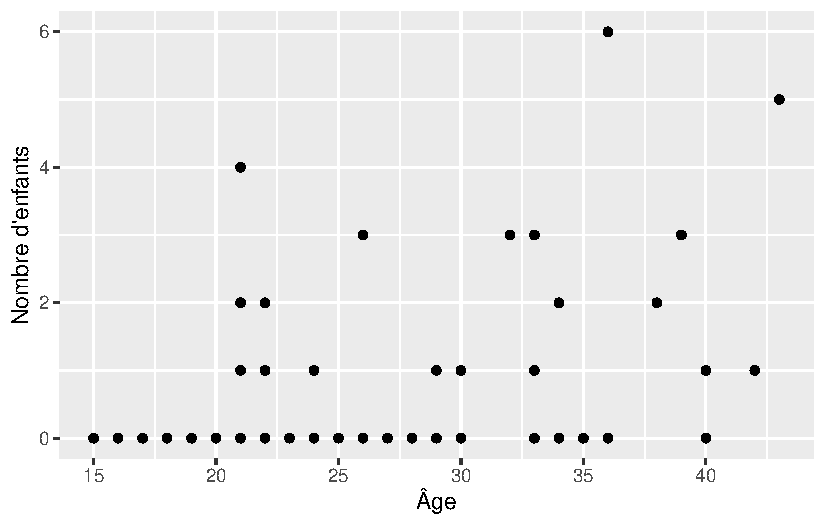
\includegraphics{projet_R_files/figure-pdf/unnamed-chunk-58-1.pdf}

}

\end{figure}

• La variable ``intention'' indique si les migrants potentiels ont
l'intention de migrer sur une échelle de 1 à 7. Estimez l'effet de
l'appartenance au groupe de traitement sur l'intention de migrer.

\begin{Shaded}
\begin{Highlighting}[]
\NormalTok{modele\_traitement}\OtherTok{\textless{}{-}}\FunctionTok{lm}\NormalTok{(intention }\SpecialCharTok{\textasciitilde{}}\NormalTok{ traitement}\DecValTok{{-}1}\NormalTok{, data)}
\NormalTok{effet\_traitement }\OtherTok{\textless{}{-}} \FunctionTok{coef}\NormalTok{(modele\_traitement)[}\StringTok{"traitement"}\NormalTok{]}

\NormalTok{mod }\OtherTok{\textless{}{-}} \FunctionTok{summary}\NormalTok{(modele\_traitement)}
\FunctionTok{bind\_rows}\NormalTok{(}
\NormalTok{  broom}\SpecialCharTok{::}\FunctionTok{tidy}\NormalTok{(mod) }
\NormalTok{)}\SpecialCharTok{\%\textgreater{}\%}
  \FunctionTok{kbl}\NormalTok{() }\SpecialCharTok{\%\textgreater{}\%}
  \FunctionTok{kable\_paper}\NormalTok{(}\AttributeTok{full\_width =} \ConstantTok{TRUE}\NormalTok{) }
\end{Highlighting}
\end{Shaded}

\begin{tabu} to \linewidth {>{\raggedright}X>{\raggedleft}X>{\raggedleft}X>{\raggedleft}X>{\raggedleft}X}
\hline
term & estimate & std.error & statistic & p.value\\
\hline
traitement & 1.982456 & 0.2977076 & 6.659071 & 0\\
\hline
\end{tabu}

• Créez un tableau de régression avec 3 modèles. La variable de résultat
est toujours ``intention''. Modèle A : Modèle vide - Effet du traitement
sur les intentions. Modèle B : Effet du traitement sur les intentions en
tenant compte de l'âge et du sexe. Modèle C : Identique au modèle B mais
en contrôlant le district. Les résultats des trois modèles doivent être
affichés dans un seul tableau.

\begin{Shaded}
\begin{Highlighting}[]
\NormalTok{modele\_a }\OtherTok{\textless{}{-}} \FunctionTok{lm}\NormalTok{(intention }\SpecialCharTok{\textasciitilde{}}\NormalTok{ traitement}\DecValTok{{-}1}\NormalTok{, data)}
\NormalTok{modele\_b }\OtherTok{\textless{}{-}} \FunctionTok{lm}\NormalTok{(intention }\SpecialCharTok{\textasciitilde{}}\NormalTok{ traitement }\SpecialCharTok{{-}}\DecValTok{1}\SpecialCharTok{+}\NormalTok{ age }\SpecialCharTok{+}\NormalTok{ sex, data )}
\NormalTok{modele\_c }\OtherTok{\textless{}{-}} \FunctionTok{lm}\NormalTok{(intention }\SpecialCharTok{\textasciitilde{}}\NormalTok{ traitement }\SpecialCharTok{{-}}\DecValTok{1}\SpecialCharTok{+}\NormalTok{ age }\SpecialCharTok{+}\NormalTok{ sex }\SpecialCharTok{+}\NormalTok{ district, data)}

\NormalTok{tableau\_regression }\OtherTok{\textless{}{-}} \FunctionTok{bind\_rows}\NormalTok{(}
\NormalTok{  broom}\SpecialCharTok{::}\FunctionTok{tidy}\NormalTok{(modele\_a) ,}
\NormalTok{  broom}\SpecialCharTok{::}\FunctionTok{tidy}\NormalTok{(modele\_b) ,}
\NormalTok{  broom}\SpecialCharTok{::}\FunctionTok{tidy}\NormalTok{(modele\_c) }
\NormalTok{)}\SpecialCharTok{\%\textgreater{}\%}
  \FunctionTok{mutate}\NormalTok{(}
    \AttributeTok{estimate =} \FunctionTok{round}\NormalTok{(estimate, }\DecValTok{3}\NormalTok{),}
    \AttributeTok{std.error =} \FunctionTok{round}\NormalTok{(std.error, }\DecValTok{3}\NormalTok{),}
    \AttributeTok{statistic =} \FunctionTok{round}\NormalTok{(statistic, }\DecValTok{3}\NormalTok{),}
    \AttributeTok{p.value =} \FunctionTok{round}\NormalTok{(p.value, }\DecValTok{3}\NormalTok{),}
    \AttributeTok{p\_value\_color =} \FunctionTok{ifelse}\NormalTok{(p.value }\SpecialCharTok{\textless{}} \FloatTok{0.05}\NormalTok{, }\StringTok{"green"}\NormalTok{, }\StringTok{""}\NormalTok{)}
\NormalTok{  )}


\NormalTok{tableau\_regression }\SpecialCharTok{\%\textgreater{}\%}
  \FunctionTok{select}\NormalTok{(}\SpecialCharTok{{-}}\NormalTok{p\_value\_color) }\SpecialCharTok{\%\textgreater{}\%} 
  \FunctionTok{kbl}\NormalTok{() }\SpecialCharTok{\%\textgreater{}\%}
  \FunctionTok{kable\_paper}\NormalTok{(}\AttributeTok{full\_width =} \ConstantTok{TRUE}\NormalTok{) }\SpecialCharTok{\%\textgreater{}\%} 
  \FunctionTok{group\_rows}\NormalTok{(}\AttributeTok{group\_label =}\StringTok{"Modèle A"}\NormalTok{, }\AttributeTok{start\_row =}\DecValTok{1}\NormalTok{, }\AttributeTok{end\_row =}\DecValTok{2}\NormalTok{) }\SpecialCharTok{\%\textgreater{}\%}
  \FunctionTok{group\_rows}\NormalTok{(}\AttributeTok{group\_label =}\StringTok{"Modèle B"}\NormalTok{, }\AttributeTok{start\_row =}\DecValTok{3}\NormalTok{, }\AttributeTok{end\_row =}\DecValTok{5}\NormalTok{) }\SpecialCharTok{\%\textgreater{}\%}
  \FunctionTok{group\_rows}\NormalTok{(}\AttributeTok{group\_label =}\StringTok{"Modèle C"}\NormalTok{, }\AttributeTok{start\_row =}\DecValTok{6}\NormalTok{, }\AttributeTok{end\_row =}\DecValTok{8}\NormalTok{) }\SpecialCharTok{\%\textgreater{}\%}
  \FunctionTok{kable\_styling}\NormalTok{() }\SpecialCharTok{\%\textgreater{}\%}
  \FunctionTok{column\_spec}\NormalTok{(}\DecValTok{1}\NormalTok{, }\AttributeTok{bold =} \ConstantTok{TRUE}\NormalTok{) }\SpecialCharTok{\%\textgreater{}\%} 
  \FunctionTok{column\_spec}\NormalTok{(}\DecValTok{5}\NormalTok{, }\AttributeTok{color =} \FunctionTok{c}\NormalTok{(tableau\_regression}\SpecialCharTok{$}\NormalTok{p\_value\_color))}
\end{Highlighting}
\end{Shaded}

\begin{tabu} to \linewidth {>{\raggedright}X>{\raggedleft}X>{\raggedleft}X>{\raggedleft}X>{\raggedleft}X}
\hline
term & estimate & std.error & statistic & p.value\\
\hline
\multicolumn{5}{l}{\textbf{Modèle A}}\\
\hline
\textbf{\hspace{1em}traitement} & 1.982 & 0.298 & 6.659 & \textcolor{green}{0.000}\\
\hline
\textbf{\hspace{1em}traitement} & -0.142 & 0.369 & -0.383 & \textcolor{}{0.702}\\
\hline
\multicolumn{5}{l}{\textbf{Modèle B}}\\
\hline
\textbf{\hspace{1em}age} & 0.083 & 0.011 & 7.536 & \textcolor{green}{0.000}\\
\hline
\textbf{\hspace{1em}sex} & -0.447 & 0.590 & -0.759 & \textcolor{}{0.450}\\
\hline
\textbf{\hspace{1em}traitement} & -0.348 & 0.366 & -0.952 & \textcolor{}{0.343}\\
\hline
\multicolumn{5}{l}{\textbf{Modèle C}}\\
\hline
\textbf{\hspace{1em}age} & 0.059 & 0.014 & 4.321 & \textcolor{green}{0.000}\\
\hline
\textbf{\hspace{1em}sex} & -0.514 & 0.571 & -0.900 & \textcolor{}{0.371}\\
\hline
\textbf{\hspace{1em}district} & 0.180 & 0.067 & 2.697 & \textcolor{green}{0.008}\\
\hline
\end{tabu}



\end{document}
